% Options for packages loaded elsewhere
\PassOptionsToPackage{unicode}{hyperref}
\PassOptionsToPackage{hyphens}{url}
%
\documentclass[
]{article}
\usepackage{amsmath,amssymb}
\usepackage{iftex}
\ifPDFTeX
  \usepackage[T1]{fontenc}
  \usepackage[utf8]{inputenc}
  \usepackage{textcomp} % provide euro and other symbols
\else % if luatex or xetex
  \usepackage{unicode-math} % this also loads fontspec
  \defaultfontfeatures{Scale=MatchLowercase}
  \defaultfontfeatures[\rmfamily]{Ligatures=TeX,Scale=1}
\fi
\usepackage{lmodern}
\ifPDFTeX\else
  % xetex/luatex font selection
\fi
% Use upquote if available, for straight quotes in verbatim environments
\IfFileExists{upquote.sty}{\usepackage{upquote}}{}
\IfFileExists{microtype.sty}{% use microtype if available
  \usepackage[]{microtype}
  \UseMicrotypeSet[protrusion]{basicmath} % disable protrusion for tt fonts
}{}
\makeatletter
\@ifundefined{KOMAClassName}{% if non-KOMA class
  \IfFileExists{parskip.sty}{%
    \usepackage{parskip}
  }{% else
    \setlength{\parindent}{0pt}
    \setlength{\parskip}{6pt plus 2pt minus 1pt}}
}{% if KOMA class
  \KOMAoptions{parskip=half}}
\makeatother
\usepackage{xcolor}
\usepackage[margin=1in]{geometry}
\usepackage{longtable,booktabs,array}
\usepackage{calc} % for calculating minipage widths
% Correct order of tables after \paragraph or \subparagraph
\usepackage{etoolbox}
\makeatletter
\patchcmd\longtable{\par}{\if@noskipsec\mbox{}\fi\par}{}{}
\makeatother
% Allow footnotes in longtable head/foot
\IfFileExists{footnotehyper.sty}{\usepackage{footnotehyper}}{\usepackage{footnote}}
\makesavenoteenv{longtable}
\usepackage{graphicx}
\makeatletter
\def\maxwidth{\ifdim\Gin@nat@width>\linewidth\linewidth\else\Gin@nat@width\fi}
\def\maxheight{\ifdim\Gin@nat@height>\textheight\textheight\else\Gin@nat@height\fi}
\makeatother
% Scale images if necessary, so that they will not overflow the page
% margins by default, and it is still possible to overwrite the defaults
% using explicit options in \includegraphics[width, height, ...]{}
\setkeys{Gin}{width=\maxwidth,height=\maxheight,keepaspectratio}
% Set default figure placement to htbp
\makeatletter
\def\fps@figure{htbp}
\makeatother
\setlength{\emergencystretch}{3em} % prevent overfull lines
\providecommand{\tightlist}{%
  \setlength{\itemsep}{0pt}\setlength{\parskip}{0pt}}
\setcounter{secnumdepth}{5}
\usepackage{caption}
\newcommand{\blandscape}{\begin{landscape}}
\newcommand{\elandscape}{\end{landscape}}
\usepackage{pdflscape}
\usepackage{booktabs}
\usepackage{longtable}
\usepackage{array}
\usepackage{multirow}
\usepackage{wrapfig}
\usepackage{float}
\usepackage{colortbl}
\usepackage{pdflscape}
\usepackage{tabu}
\usepackage{threeparttable}
\usepackage{threeparttablex}
\usepackage[normalem]{ulem}
\usepackage{makecell}
\usepackage{xcolor}
\ifLuaTeX
  \usepackage{selnolig}  % disable illegal ligatures
\fi
\usepackage{bookmark}
\IfFileExists{xurl.sty}{\usepackage{xurl}}{} % add URL line breaks if available
\urlstyle{same}
\hypersetup{
  pdftitle={Model-based index development for Bering Sea and Aleutian Islands Chionoecetes crab stocks},
  hidelinks,
  pdfcreator={LaTeX via pandoc}}

\title{Model-based index development for Bering Sea and Aleutian Islands \emph{Chionoecetes} crab stocks}
\usepackage{etoolbox}
\makeatletter
\providecommand{\subtitle}[1]{% add subtitle to \maketitle
  \apptocmd{\@title}{\par {\large #1 \par}}{}{}
}
\makeatother
\subtitle{Update for Crab Plan Team}
\author{Emily Ryznar\\
NOAA Fisheries\\
\href{mailto:emily.ryznar@noaa.gov}{\nolinkurl{emily.ryznar@noaa.gov}}}
\date{May 2025}

\begin{document}
\maketitle

\pagenumbering{arabic}

\section*{Introduction}\label{introduction}
\addcontentsline{toc}{section}{Introduction}

The goal of this investigation was to develop spatiotemporal model-based indices of abundance for two Bering Sea and Aleutian Islands (BSAI) crab stocks: Tanner crab (\emph{Chionoecetes bairdi}) and snow crab (\emph{Chionoecetes opilio}). St.~Matthew Island blue king crab (\emph{Paralithodes platypus}) and Norton Sound red king crab (\emph{Paralithodes camtschaticus}) model indices are presented in separate documents (Stern et al.~2025a; Stern 2025b). Research suggests that spatiotemporal model-based indices can be more robust to survey changes than design-based indices, though the models must be well-specified (Yalcin et al.~2023). Spatiotemporal model-based indices are used in North Pacific Fishery Management Council (NPFMC) groundfish stock assessments for species including eastern Bering Sea (EBS) walleye pollock (\emph{Gadus chalcogrammus}) and EBS Pacific cod (\emph{Gadus macrocephalus}), both of which use the vector-autoregressive spatial temporal (VAST) approach (Thorson 2019) to produce indices used in the assessments (Ianelli et al.~2024; Barbeaux et al.~2024). Previous BSAI crab stock assessments have presented models using spatiotemporal model-based indices (e.g., Ianelli et al.~2017), although these models were not accepted for harvest specifications (SSC 2017).

Biomass and abundance estimates were generated using the R package \emph{sdmTMB} (Anderson et al.~2022), which uses geostatistical time series data to estimate spatial and spatiotemporal generalized linear mixed effects models. This approach allows for index standardization when the set of stations surveyed is not consistent across years: one can generate a spatial grid that covers the area of interest, predict from the model onto that grid, and sum the predicted abundance/biomass to obtain an area-weighted index that is independent of sampling locations (Anderson et al.~2022).

The two stock assessments for the crab stocks presented here use data from the National Marine Fisheries Service (NMFS) eastern Bering Sea (EBS) bottom trawl survey (Stockhausen 2024; Szuwalski 2024). Due to this, spatiotemporal model-based index development is expected to confer advantages for each stock. Standardizing the survey indices could allow the assessment to use the existing survey data more rigorously. Throughout its history, the NMFS EBS trawl survey has undergone changes in its spatial footprint, including recently dropping the high sampling density ``corner stations'' near St.~Matthew Island from 2024 onward (DeFilippo et al.~2023); index standardization would allow assessments to continue using the full time series of data despite these changes.

Spatiotemporal index standardization can also be accomplished using VAST. However, compared to \emph{sdmTMB}, VAST is often criticized for having a difficult user interface, slower estimation times, and less-flexible model specification. Therefore, \emph{sdmTMB} is primarily used the following index standardization.

\section*{Methods}\label{methods}
\addcontentsline{toc}{section}{Methods}

Models were fit using the R package \emph{sdmTMB}. A number of decision points arise in \emph{sdmTMB}, including:

\begin{itemize}
\item
  The resolution of the spatial mesh used in fitting the model. A higher number of knots, specified when creating the spatial mesh using the make\_mesh() function, indicates a higher resolution mesh.
\item
  The spatiotemporal random fields estimation method. The spatiotemporal random fields can be estimated as independent and identically distributed (IID), first-order autoregressive (AR1), a random walk, or fixed at zero. The spatial random fields are estimated for each time slice, the period of which is specified in the model (e.g., time = year).
\item
  The model family. Many options exist, including tweedie(), delta\_gamma(), and delta\_lognormal().
\end{itemize}

For each stock, a range of models were ran to examine the effects of choices at each of these decision points on model predictions. After fitting models, the following steps for model evaluation were used:

\begin{itemize}
\tightlist
\item
  First, model convergence was evaluated using the sdmTMB::sanity() function. Output of this function for a model that passes all sanity checks is displayed as follows:
\end{itemize}

\(\checkmark\) Non-linear minimizer suggests successful convergence

\(\checkmark\) Hessian matrix is positive definite

\(\checkmark\) No extreme or very small eigenvalues detected

\(\checkmark\) No gradients with respect to fixed effects are \textgreater= 0.001

\(\checkmark\) No fixed-effect standard errors are NA

\(\checkmark\) No standard errors look unreasonably large

\(\checkmark\) No sigma parameters are \textless{} 0.01

\(\checkmark\) No sigma parameters are \textgreater{} 100

\(\checkmark\) Range parameter doesn't look unreasonably large

\begin{itemize}
\item
  If a model passed all the sanity checks, the R package \emph{DHARMa} (Hartig 2022) was used to calculate the DHARMa residuals using the function DHARMa::dharma\_residuals(). Models that did not pass the sanity checks were excluded from further consideration.
\item
  DHARMa residual Q-Q plots and evidence of quantile deviations, under- or overdispersion, outliers, and zero- inflation were examined using the functions DHARMa::testQuantiles(), DHARMa::testDispersion(), DHARMa::testOutliers(), and DHARMa::testZeroInflation(), respectively. Plots of DHARMa residuals were examined over space and time for potential patterns of autocorrelation.
\item
  Model predictive skill was evaluated (the predictive ability of the model for new observations; Anderson \emph{et al.} 2024) using the cross validation function sdmTMB\_cv(). This function measures model predictive skill by holding out subsets of the data in turn and using each as a test set. These subsets of data are termed ``folds''. To compare models, cross validation was conducted with three folds for each model then the model's summed log-likelihood value was extracted, which represents the model's predictive density. Predictive density values closer to zero indicate better out-of-sample predictive skill. Model-predicted indices were also plotted against observed values and examined for goodness-of-fit.
\item
  Finally, model-predicted indices were compared using the best model framework for each stock with indices generated in VAST (when available) using a comparable framework to evaluate potential differences in index generation between model algorithms.
\end{itemize}

\subsection*{Tanner crab}\label{tanner-crab}
\addcontentsline{toc}{subsection}{Tanner crab}

Abundance and biomass data collected from the NMFS EBS bottom trawl survey (1975-2024) were utilized to fit Tanner crab models in \emph{sdmTMB}. Sex-maturity categories included all males combined, immature females, and mature females to align with the stock assessment model, and data were filtered to only include crab with a carapace width greater than or equal to 25mm. As the survey gear and methods were standardized in 1982 (Stauffer 2004), separate models were fit to data before 1982 and data in and after 1982 for each sex-size/maturity category. To evaluate decision points for model formulations, models were fit using a 50-knot, 90-knot, and 120-knot mesh (Figures \ref{fig:bairdi-50-mesh} - \ref{fig:bairdi-120-mesh}), a Tweedie or delta-gamma model family, and a IID spatiotemporal random field. Models fit using the delta-lognormal family did not pass initial model sanity checks and models using an AR1 or random walk spatiotemporal random field did not converge. Therefore, these frameworks are not discussed further. The best model framework was used to predict Tanner crab abundance and biomass on an EBS-wide survey grid (Figure \ref{fig:bairdi-EBS-grid}), a grid encompassing the EBS area west of 166° (for the Tanner West stock; Figure \ref{fig:bairdi-west-grid}, Appendix), and a grid encompassing the EBS area east of 166° (for the Tanner East stock; Figure \ref{fig:bairdi-east-grid}, Appendix). Each prediction grid was a resolution of 5 km\(^2\).

\subsection*{Snow crab}\label{snow-crab}
\addcontentsline{toc}{subsection}{Snow crab}

Biomass data collected from the NMFS EBS (1980-2024) and northern Bering Sea (NBS; 2010, 2017-2019, 2021-2023) bottom trawl survey was used to fit snow crab models in \emph{sdmTMB}. Sex-size/maturity categories included males greater than 95mm and mature females to align with the stock assessment model. To evaluate decision points for model formulations, models were fit using a 50-knot, 90-knot, and 120-knot mesh for EBS data only (Figure \ref{fig:snow-EBS-mesh}) and EBS-NBS data combined (Figure \ref{fig:snow-NBS-mesh}), a Tweedie or delta-gamma model family, and a IID spatiotemporal random field for EBS-only models. An AR1 random field was used for models fit using EBS and NBS data, as this method is suitable for data where years are not continuous, as is the case for NBS survey data. The best model framework was then used to predict snow crab biomass on an EBS-wide survey grid (Figure \ref{fig:snow-EBS-grid}). The prediction grid was a resolution of 5 km\(^2\). Models initially were fit using EBS data only then compared to models fit with both EBS and NBS data to evaluate if including NBS data enhanced model performance.

\section*{Results}\label{results}
\addcontentsline{toc}{section}{Results}

\subsection*{Tanner crab}\label{tanner-crab-1}
\addcontentsline{toc}{subsection}{Tanner crab}

\subsubsection*{Model diagnostics}\label{model-diagnostics}
\addcontentsline{toc}{subsubsection}{Model diagnostics}

All models passed sanity checks. Model diagnostics using DHARMa residuals varied among the number of knots specified in the mesh (50, 90, 120), model family (Tweedie, delta-gamma), and data period (pre-1982, 1982 onward) for both abundance (Table \ref{tab:bairdi-abund-modeleval}) and biomass (Table \ref{tab:bairdi-bio-modeleval}) models. For male abundance, a model using a delta-gamma distribution and 50 knots performed the best for both periods in terms of the greatest log-likelihood, with only the post-1982 model showing evidence of outliers, zero-inflation, and quantile deviations. However, this was true regardless of the model family or number of knots used, and this pattern was consistent across other sex-maturity categories. For immature female abundance, a delta-gamma model had the largest log-likelihood across periods, with models using 90 and 50 knots performing best pre-1982 and post-1982, respectively. The best model pre-1982 showed evidence of quantile deviation and dispersion, whereas the best model post-1982 showed evidence of outliers, zero-inflation, and quantile deviation. Contrasting the other two sex-maturity categories, the Tweedie family had the largest log-likelihood for mature female abundance, with 90 and 50 knots performing best pre-1982 and post-1982, respectively. The pre-1982 Tweedie model only showed evidence of zero-inflation, whereas the post-1982 Tweedie model showed evidence of outliers, dispersion, zero-inflation, and quantile deviation.

As with male abundance, a delta-gamma model using 50 knots had the largest log-likelihood for male biomass pre- and post-1982. Models for both periods showed evidence of quantile deviation, dispersion, and outliers, where just the post-1982 model also showed evidence of zero-inflation as was true for other models in this period. For immature female biomass, a Tweedie model using 90 and 50 knots for pre- and post-1982 had the greatest log-likelihood. While the pre-1982 Tweedie model had the largest log-likelihood, it showed evidence of dispersion and zero-inflation whereas the next-best model, a delta-gamma using 90 knots, did not. For immature female biomass post-1982, Tweedie and delta-gamma models using 50 knots had the largest and very similar log-likelihoods, with the Tweedie model showing evidence of quantile deviation, dispersion, outliers, and zero-inflation where the delta-gamma model did not show evidence of dispersion. A similar pattern was seen in diagnostics for mature female biomass models, where Tweedie models using 50 knots had the largest but very similar log-likelihood values to delta-gamma models using 50 knots across both periods. The pre-1982 50-knot Tweedie model showed evidence of dispersion, outliers, and zero-inflation, whereas the 50-knot delta-gamma model did not. The post-1982 50-knot Tweedie model exhibited evidence of all diagnostics, whereas the 50-knot delta-gamma model did not show evidence of dispersion.

Accounting for strong model performance across sex-maturity categories, periods, and response (abundance/biomass), a delta-gamma model family and a 50-knot mesh was selected as a parsimonious model framework for prediction. DHARMa residuals for these models across sex-maturity categories and periods did not strongly diverge from the 1-1 line (Figures \ref{fig:DHARMa-abund-QQ-50} - \ref{fig:DHARMa-bio-QQ-50}) despite some evidence of quantile dispersion. In addition, DHARMa residuals for these models did not show evidence of spatiotemporal autocorrelation (Figures \ref{fig:DHARMa-abund-spat-50-male} - \ref{fig:DHARMa-bio-spat-50-matfem}).

\subsubsection*{Predicted abundance and biomass}\label{predicted-abundance-and-biomass}
\addcontentsline{toc}{subsubsection}{Predicted abundance and biomass}

Heat maps of EBS-wide predicted abundance for Tanner crab males, immature females, and mature females are shown in figures \ref{fig:spatpred-abund-50-male} - \ref{fig:spatpred-abund-50-matfem}, respectively, using our chosen model framework (delta-gamma, 50 knots). Heat maps of EBS-wide predicted biomass for Tanner crab males, immature females, and mature females are shown in figures \ref{fig:spatpred-bio-50-male} - \ref{fig:spatpred-bio-50-matfem}. Abundance and biomass heat maps for Tanner crab west and east of 166° are shown in Appendix figures \ref{fig:spatpred-abund-50-maleW} - \ref{fig:spatpred-bio-50-matfemW} and figures \ref{fig:spatpred-abund-50-maleE} - \ref{fig:spatpred-bio-50-matfemE}, respectively.

\subsubsection*{Predicted index fits to observations}\label{predicted-index-fits-to-observations}
\addcontentsline{toc}{subsubsection}{Predicted index fits to observations}

The EBS-wide model-predicted indices using a delta-gamma family varied in their fits to survey abundance (Figure \ref{fig:bairdi-abund-index}) and biomass observations (Figure \ref{fig:bairdi-bio-index}) across sex-maturity categories and between model fitting periods. Across sex-maturity categories, model fits with different knots were most variable before 1982, which could be due to high variability in the spatial footprint of the survey in this period. In this period, uncertainty was generally greater in indices predicted using 50 knots, with the majority of survey observations points and associated uncertainty overlapping with model predicted values and uncertainty. From 1982 onward, indices predicted at different knots are less variable compared with each other, with models using 50 knots generally exhibiting greater uncertainty than 90 and 120 knots. As before, the majority of survey observations points and associated uncertainty overlap with model predicted values and uncertainty across knot specifications. Similar patterns across knots and sex-maturity categories were seen for predicted abundance and biomass indices for Tanners west and east of 166° (Figures \ref{fig:Westbairdi-abund-index} - \ref{fig:Eastbairdi-bio-index}, Appendix).

\subsubsection*{\texorpdfstring{Comparison of \emph{sdmTMB} with VAST}{Comparison of sdmTMB with VAST}}\label{comparison-of-sdmtmb-with-vast}
\addcontentsline{toc}{subsubsection}{Comparison of \emph{sdmTMB} with VAST}

For the EBS, abundance and biomass indices were similar between \emph{sdmTMB} and VAST estimates (Figures \ref{fig:EBSbairdi-abund-compare} - \ref{fig:EBSbairdi-bio-compare}). Across sex-maturity categories, the greatest differences in \emph{sdmTMB} and VAST estimates were in the pre-1982 period, with \emph{sdmTMB} estimates generally exhibiting greater uncertainty in this period. Among sex-maturity categories, the greatest difference in estimates were for mature females, where \emph{sdmTMB} estimates were generally slightly higher than VAST but still tracking the observed survey values. Similar patterns were seen in \emph{sdmTMB} and VAST estimates for Tanner crab west of 166° (Figures \ref{fig:Westbairdi-abund-compare} - \ref{fig:Westbairdi-bio-compare}, Appendix) and east of 166°(Figures \ref{fig:Eastbairdi-abund-compare} - \ref{fig:Eastbairdi-bio-compare}, Appendix).

\subsection*{Snow crab}\label{snow-crab-1}
\addcontentsline{toc}{subsection}{Snow crab}

\subsubsection*{Model diagnostics}\label{model-diagnostics-1}
\addcontentsline{toc}{subsubsection}{Model diagnostics}

All models passed sanity checks. Model diagnostics using DHARMa residuals varied among the number of knots specified in the mesh (50, 90, 120) and model family (Tweedie, delta-gamma) for biomass models (Table \ref{tab:snow-bio-modeleval}). For male biomass \textgreater95mm using EBS data only, a delta-gamma model using 90 knots had the largest log-likelihood. This model showed evidence of quantile deviation, outliers, and zero-inflation which was not improved when models were fit using 50 or 120 knots or a Tweedie distribution. For mature female biomass using EBS data only, a delta-gamma model using 50 knots had the greatest log-likelihood. As with males, this model showed evidence of quantile deviation, outliers, and zero-inflation which was not improved using a different numbers of knots or distribution. For male biomass fit with EBS and NBS data, a delta-gamma model using 90 knots had the largest log-likelihood. However, as with the EBS-only models, this model showed evidence of quantile deviation, outliers, and zero-inflation regardless of the number of knots. For mature female biomass fit with EBS and NBS data, a model fit with 50 knots had the largest log-likelihood but still showed evidence of quantile deviation, outliers, and zero-inflation.

A delta-gamma model family was selected along with a 90-knot mesh for males \textgreater95mm and a 50-knot mesh for mature females as the top-performing model framework for each sex-size/maturity category. DHARMa residuals for these models fit using EBS data only as well as models using EBS and NBS data did not strongly diverge from the 1-1 line despite some evidence of quantile dispersion (Figure \ref{fig:snow-DHARMa-QQ-EBSNBS}). Spatial DHARMa residuals for these models using EBS-only data did not show evidence of spatiotemporal autocorrelation (Figures \ref{fig:snow-DHARMa-spat-90-male95-EBS} - \ref{fig:snow-DHARMa-spat-50-matfem-EBS}). However, models using these knots and both EBS and NBS data displayed evidence of spatiotemporal autocorrelation, specifically in the NBS portion of the grid for mature female predictions (Figures \ref{fig:snow-DHARMa-spat-90-male95-EBSNBS} - \ref{fig:snow-DHARMa-spat-50-matfem-EBSNBS}).

\subsubsection*{Predicted abundance and biomass}\label{predicted-abundance-and-biomass-1}
\addcontentsline{toc}{subsubsection}{Predicted abundance and biomass}

Heat maps of EBS-wide predicted biomass for snow crab males \textgreater95mm and mature females using EBS data only are shown in figures \ref{fig:snow-spatpred-bio-90-male-EBS} - \ref{fig:snow-spatpred-bio-50-matfem-EBS}, respectively, using our chosen model framework (delta-gamma, 90 knots for males \textgreater{} 95mm, 50 knots for mature females). Heat maps of EBS-wide predicted biomass using EBS and NBS data are shown in figures \ref{fig:snow-spatpred-bio-90-male-EBSNBS} - \ref{fig:snow-spatpred-bio-50-matfem-EBSNBS}

\subsubsection*{Predicted index fits to observations}\label{predicted-index-fits-to-observations-1}
\addcontentsline{toc}{subsubsection}{Predicted index fits to observations}

The EBS-wide model-predicted indices using a delta-gamma family and EBS-only data varied in their fits to survey biomass observations (Figure \ref{fig:snow-bio-index-EBS}) between sex-size/maturity categories and the number of knots used in the model mesh. For males \textgreater{} 95mm, there was generally greater uncertainty in model indices before \textasciitilde2000 regardless of knot specification, which corresponds to survey observations. Indices and associated confidence intervals across all knot specifications overlapped the confidence intervals of the survey observations. Therefore, there were no strong differences in performance among the number of knots for male indices. Indices for mature females displayed greater uncertainty than for males, which also corresponds with greater uncertainty in the survey observations. Mature female estimated biomass using 50 knots was generally slightly lower than biomass using 90 or 120 knots. The 50-knot index tracked survey observations more so than the other knot specifications, overlapping the survey values and associated uncertainty each year.

Comparing indices generated from the best models for males \textgreater{} 95mm (delta-gamma, 90 knots) and mature females (delta-gamma, 50 knots) built using EBS data only and EBS and NBS data combined illustrated different alignment with the survey data between sex-size/maturity categories (Figure \ref{fig:snow-bio-index-EBSNBS}). For males, biomass indices and associated uncertainty were very similar to each other and survey observations across the time series regardless of what data region was used to fit the models, though models using EBS-NBS data were slightly better aligned with survey observations. Biomass indices using EBS data only were slightly higher across years with slightly larger confidence intervals than indices using EBS and NBS data. For mature females, the biomass predicted from the EBS data only model is generally higher across the time series and seems to track the survey data better earlier in the time series, specifically pre-1990. Post 1990, the index from the model that also includes NBS data follows the survey observations more closely and generally with less uncertainty, though the indices and associated confidence intervals overlap the survey observations most years regardless of the data region used to fit the models.

\subsubsection*{\texorpdfstring{Comparison of \emph{sdmTMB} with VAST}{Comparison of sdmTMB with VAST}}\label{comparison-of-sdmtmb-with-vast-1}
\addcontentsline{toc}{subsubsection}{Comparison of \emph{sdmTMB} with VAST}

Updated VAST indices for snow crab are not available, so we only present sdmTMB indices.

\section*{Recommended models}\label{recommended-models}
\addcontentsline{toc}{section}{Recommended models}

For Tanner crab, we recommend a delta-gamma model using a 50-knot mesh as these were consistently top-performing models across sex-maturity categories and periods. However, different best models could be selected by sex-maturity category and fitting period such as delta-gamma models using 90 knots.

For snow crab, we recommend a delta-gamma model using a 90-knot mesh for males \textgreater95mm and a delta-gamma model using a 50-knot mesh for mature females, as these were the top-performing models for each sex-size/maturity category in terms of log-likelihood, other residual diagnostics, and index similarity with survey data. While indices from models using combined EBS-NBS data were slightly more aligned with survey observations than models just using EBS data, the spatiotemporal autocorrelation evident in NBS DHARMa residuals may be problematic. Further analysis is needed to evaluate the extent of autocorrelation.

\section*{Acknowledgements}\label{acknowledgements}
\addcontentsline{toc}{section}{Acknowledgements}

The authors thank Katie Palof and Mike Litzow for their support and feedback on this work.

\clearpage

\section*{References}\label{references}
\addcontentsline{toc}{section}{References}

Anderson, S.C., Ward, E.J., English, P.A., Barnett, L.A.K. 2022. sdmTMB: An R package for fast, flexible, and user-friendly generalized linear mixed effects models with spatial and spatiotemporal random fields. bioRxiv.

Anderson, S.C., Ward, E.J., English, P.A., Barnett, L.A.K., Thorson, J.T. 2024. Cross-validation for model evaluation and comparison. Retrieved from \url{https://pbs-assess.github.io/sdmTMB/articles/cross-validation.html}.

Barbeaux, S.J., L. Barnett, P. Hulson, J. Nielsen, S.K. Shotwell, E. Siddon, I. Spies. 2024. Assessment of the Pacific cod stock in the Eastern Bering Sea. In: Stock Assessment and Fishery Evaluation report for the Groundfish Resources of the Bering Sea/Aleutian Islands regions. North Pacific Fishery Management Council, Anchorage, AK.

DeFilippo, L., S. Kotwicki, L. Barnett, J. Richar, M.A.~Litzow, W.T. Stockhausen, K. Palof. 2023. Evaluating the impacts of reduced sampling density in a systematic fisheries-independent survey design. Frontiers in Marine Science 10:1219283.

Hartig, F. 2022. DHARMa: Residual Diagnostics for Hierarchical (Multi-Level / Mixed) Regression Models. R package version 0.4.6, \url{https://CRAN.R-project.org/package=DHARMa}.

Ianelli, J., D. Webber, J. Zheng, A. Letaw. 2017. Saint Matthew Island blue king crab stock assessment 2017. In: Stock Assessment and Fishery Evaluation Report for the King and Tanner Crab Fisheries of the Bering Sea and Aleutian Islands: 2017 Final Crab SAFE. North Pacific Fishery Management Council, Anchorage AK.

Ianelli, J., T. Honkalehto, S. Wassermann, A. McCarthy, S. Steinessen, C. McGilliard, E. Siddon. 2024. Assessment of walleye pollock in the eastern Bering Sea. In: Stock Assessment and Fishery Evaluation report for the Groundfish Resources of the Bering Sea/Aleutian Islands regions. North Pacific Fishery Management Council, Anchorage, AK.

SSC. 2017. Scientific and Statistical Committee report to the North Pacific Fishery Management Council, October 2nd-4th, 2017. North Pacific Fishery Management Council, Anchorage, AK.

Stauffer, G.A. 2004. NOAA protocols for groundfish bottom trawl surveys of the Nation's fishery resources. U.S. Dep. Commer., NOAA Tech. Memo. NMFS-F/SPO-65, 205p.

Stern, C., Ryznar, E., and J. Richar. 2025a. Spatiotemporal model-based index development for Bering Sea and Aleutian Islands crab stocks: Update for Crab Plan Team modeling workshop. BSAI Crab Plan Team modeling workshop, January 2025. North Pacific Fishery Management Council, Anchorage AK.

Stern, C. 2025b. Spatiotemporal model-based survey indices of abundance for Norton Sound red king crab. BSAI Crab Plan Team, May 2025. North Pacific Fishery Management Council, Anchorage AK.

Stockhausen, W.T. 2024. 2024 stock assessment and fishery evaluation report for the Tanner crab fisheries of the Bering Sea and Aleutians Islands regions. In: Stock Assessment and Fishery Evaluation Report for the King and Tanner Crab Fisheries of the Bering Sea and Aleutian Islands: 2024 Final Crab SAFE. North Pacific Fishery Management Council, Anchorage AK.

Szuwalski, C. 2024. An assessment for eastern Bering Sea snow crab: 2024 Final Crab SAFE. North Pacific Fishery Management Council, Anchorage AK.

Thorson, J.T. 2019. Guidance for decisions using the vector autoregressive spatio-temporal (VAST) package in stock, ecosystem, habitat, and climate assessments. Fisheries Research 210:143-161. \url{https://doi.org/10.1016/j.fishres.2018.10.013}

Yalcin, S., S.C. Anderson, P.M. Regular, P.A. English. 2023. Exploring the limits of spatiotemporal and design-based index standardization under reduced survey coverage. ICES Journal of Marine Sciences 80:2368-2379. \url{https://doi.org/10.1093/icesjms/fsad155}

\clearpage

\section*{Tables}\label{tables}
\addcontentsline{toc}{section}{Tables}

\begin{table}
\centering\centering
\caption{\label{tab:bairdi-abund-modeleval}Tanner crab diagnostic values for abundance models fit with Tweedie or delta gamma families and a spatial resolution of 50, 90, or 120 knots across sex-size maturity categories and model-fitting periods (pre-1982, during or after 1982). Log-likelihood values were estimated using the cross-validation function in sdmTMB with three folds. Quantile, dispersion, outlier, and zero-inflation diagnostics were estimated from DHARMa residuals, with values below 0.05 indicating significant metrics. Values are ordered within sex-size maturity category and period by decreasing log-likelihood.}
\centering
\resizebox{\ifdim\width>\linewidth\linewidth\else\width\fi}{!}{
\begin{tabular}[t]{lllrrrrrr}
\toprule
Category & Period & Family & Knots & Log-likelihood & Quantiles & Dispersion & Outliers & Zero-inflation\\
\midrule
Immature Female & <1982 & Delta-gamma & 90 & -6371.5 & 0.0 & 0.0 & 0.5 & 0.5\\
Immature Female & <1982 & Tweedie & 90 & -6475.4 & 0.0 & 0.0 & 0.0 & 0.1\\
Immature Female & <1982 & Tweedie & 120 & -6666.0 & 0.1 & 0.0 & 0.4 & 0.2\\
Immature Female & <1982 & Delta-gamma & 50 & -6716.3 & 0.0 & 0.2 & 0.2 & 0.0\\
Immature Female & <1982 & Tweedie & 50 & -6850.9 & 0.1 & 0.0 & 0.1 & 0.1\\
\addlinespace
Immature Female & <1982 & Delta-gamma & 120 & -6907.8 & 0.0 & 0.0 & 0.1 & 0.1\\
Immature Female & >=1982 & Delta-gamma & 50 & -53281.6 & 0.0 & 0.1 & 0.0 & 0.0\\
Immature Female & >=1982 & Tweedie & 50 & -53380.1 & 0.0 & 0.0 & 0.0 & 0.0\\
Immature Female & >=1982 & Tweedie & 90 & -53543.3 & 0.0 & 0.0 & 0.0 & 0.0\\
Immature Female & >=1982 & Delta-gamma & 90 & -53553.8 & 0.0 & 0.2 & 0.0 & 0.0\\
\addlinespace
Immature Female & >=1982 & Tweedie & 120 & -53722.7 & 0.0 & 0.0 & 0.0 & 0.0\\
Immature Female & >=1982 & Delta-gamma & 120 & -53852.8 & 0.0 & 0.7 & 0.0 & 0.0\\
Male & <1982 & Delta-gamma & 50 & -9256.2 & 0.4 & 0.5 & 0.1 & 0.4\\
Male & <1982 & Tweedie & 90 & -9339.9 & 0.0 & 0.0 & 0.0 & 0.1\\
Male & <1982 & Delta-gamma & 90 & -9349.7 & 0.0 & 0.1 & 0.5 & 0.3\\
\addlinespace
Male & <1982 & Tweedie & 120 & -9397.7 & 0.0 & 0.0 & 0.0 & 0.0\\
Male & <1982 & Delta-gamma & 120 & -9398.7 & 0.1 & 0.5 & 0.4 & 0.1\\
Male & <1982 & Tweedie & 50 & -9540.7 & 0.0 & 0.0 & 0.0 & 0.0\\
Male & >=1982 & Delta-gamma & 50 & -76006.3 & 0.0 & 0.1 & 0.0 & 0.0\\
Male & >=1982 & Tweedie & 50 & -76072.9 & 0.0 & 0.0 & 0.0 & 0.0\\
\addlinespace
Male & >=1982 & Tweedie & 90 & -76229.4 & 0.0 & 0.0 & 0.0 & 0.0\\
Male & >=1982 & Delta-gamma & 90 & -76277.7 & 0.0 & 0.1 & 0.0 & 0.0\\
Male & >=1982 & Tweedie & 120 & -76318.2 & 0.0 & 0.0 & 0.0 & 0.0\\
Male & >=1982 & Delta-gamma & 120 & -76509.5 & 0.0 & 0.1 & 0.0 & 0.0\\
Mature Female & <1982 & Tweedie & 90 & -6089.8 & 0.1 & 0.4 & 0.1 & 0.0\\
\addlinespace
Mature Female & <1982 & Delta-gamma & 90 & -6097.3 & 0.0 & 0.8 & 0.5 & 0.6\\
Mature Female & <1982 & Delta-gamma & 50 & -6097.4 & 0.0 & 0.4 & 0.0 & 0.0\\
Mature Female & <1982 & Delta-gamma & 120 & -6108.3 & 0.2 & 0.3 & 0.1 & 0.0\\
Mature Female & <1982 & Tweedie & 120 & -6132.7 & 0.0 & 0.0 & 0.8 & 0.0\\
Mature Female & <1982 & Tweedie & 50 & -6189.4 & 0.1 & 0.0 & 0.0 & 0.0\\
\addlinespace
Mature Female & >=1982 & Tweedie & 50 & -43560.9 & 0.0 & 0.0 & 0.0 & 0.0\\
Mature Female & >=1982 & Delta-gamma & 50 & -43625.4 & 0.0 & 0.0 & 0.0 & 0.0\\
Mature Female & >=1982 & Delta-gamma & 90 & -43803.8 & 0.0 & 0.0 & 0.0 & 0.0\\
Mature Female & >=1982 & Delta-gamma & 120 & -43943.3 & 0.0 & 0.0 & 0.0 & 0.0\\
Mature Female & >=1982 & Tweedie & 90 & -43837.0 & 0.0 & 0.0 & 0.0 & 0.0\\
\addlinespace
Mature Female & >=1982 & Tweedie & 120 & -44059.6 & 0.0 & 0.0 & 0.0 & 0.0\\
\bottomrule
\end{tabular}}
\end{table}

\clearpage

\begin{table}
\centering\centering
\caption{\label{tab:bairdi-bio-modeleval}Tanner crab diagnostic values for biomass models fit with Tweedie or delta gamma families and a spatial resolution of 50, 90, or 120 knots across sex-size maturity categories and model-fitting periods (pre-1982, during or after 1982). Log-likelihood values were estimated using the cross-validation function in sdmTMB with three folds. Quantile, dispersion, outlier, and zero-inflation diagnostics were estimated from DHARMa residuals, with values below 0.05 indicating significant metrics. Values are ordered within sex-size maturity category and period by decreasing log-likelihood.}
\centering
\resizebox{\ifdim\width>\linewidth\linewidth\else\width\fi}{!}{
\begin{tabular}[t]{lllrrrrrr}
\toprule
Category & Period & Family & Knots & Log-likelihood & Quantiles & Dispersion & Outliers & Zero-inflation\\
\midrule
Immature Female & <1982 & Tweedie & 90 & -6356.8 & 0.2 & 0.0 & 1.0 & 0.0\\
Immature Female & <1982 & Delta-gamma & 90 & -6514.3 & 0.1 & 0.3 & 0.4 & 0.1\\
Immature Female & <1982 & Delta-gamma & 120 & -6630.5 & 0.0 & 0.1 & 0.9 & 0.3\\
Immature Female & <1982 & Tweedie & 120 & -6823.7 & 0.1 & 0.1 & 0.7 & 0.8\\
Immature Female & <1982 & Delta-gamma & 50 & -6874.7 & 0.0 & 0.0 & 0.0 & 0.0\\
\addlinespace
Immature Female & <1982 & Tweedie & 50 & -7246.5 & 0.0 & 0.0 & 0.2 & 0.3\\
Immature Female & >=1982 & Tweedie & 50 & -53292.8 & 0.0 & 0.0 & 0.0 & 0.0\\
Immature Female & >=1982 & Delta-gamma & 50 & -53303.1 & 0.0 & 0.1 & 0.0 & 0.0\\
Immature Female & >=1982 & Tweedie & 90 & -53587.3 & 0.0 & 0.0 & 0.0 & 0.0\\
Immature Female & >=1982 & Delta-gamma & 120 & -53639.8 & 0.0 & 1.0 & 0.0 & 0.0\\
\addlinespace
Immature Female & >=1982 & Tweedie & 120 & -53652.8 & 0.0 & 0.0 & 0.0 & 0.0\\
Immature Female & >=1982 & Delta-gamma & 90 & -53652.9 & 0.0 & 0.9 & 0.0 & 0.0\\
Male & <1982 & Delta-gamma & 50 & -9275.5 & 0.0 & 0.0 & 0.0 & 0.3\\
Male & <1982 & Tweedie & 90 & -9295.3 & 0.0 & 0.0 & 0.1 & 0.3\\
Male & <1982 & Tweedie & 50 & -9309.6 & 0.0 & 0.0 & 0.0 & 0.1\\
\addlinespace
Male & <1982 & Delta-gamma & 120 & -9343.0 & 0.0 & 0.0 & 0.1 & 0.7\\
Male & <1982 & Delta-gamma & 90 & -9349.5 & 0.0 & 0.0 & 0.4 & 0.0\\
Male & <1982 & Tweedie & 120 & -9422.2 & 0.0 & 0.0 & 0.5 & 0.6\\
Male & >=1982 & Delta-gamma & 50 & -75992.4 & 0.0 & 0.0 & 0.0 & 0.0\\
Male & >=1982 & Tweedie & 50 & -76031.1 & 0.0 & 0.0 & 0.0 & 0.0\\
\addlinespace
Male & >=1982 & Delta-gamma & 90 & -76307.0 & 0.0 & 0.0 & 0.0 & 0.0\\
Male & >=1982 & Tweedie & 120 & -76345.7 & 0.0 & 0.0 & 0.0 & 0.0\\
Male & >=1982 & Delta-gamma & 120 & -76382.0 & 0.0 & 0.0 & 0.0 & 0.0\\
Male & >=1982 & Tweedie & 90 & -76489.4 & 0.0 & 0.0 & 0.0 & 0.0\\
Mature Female & <1982 & Tweedie & 50 & -6101.9 & 0.2 & 0.0 & 0.0 & 0.0\\
\addlinespace
Mature Female & <1982 & Delta-gamma & 50 & -6108.2 & 0.2 & 0.1 & 0.1 & 0.5\\
Mature Female & <1982 & Delta-gamma & 120 & -6108.8 & 0.0 & 0.4 & 0.4 & 0.4\\
Mature Female & <1982 & Delta-gamma & 90 & -6134.0 & 0.0 & 0.3 & 0.4 & 0.6\\
Mature Female & <1982 & Tweedie & 90 & -6135.2 & 0.2 & 0.9 & 0.5 & 0.0\\
Mature Female & <1982 & Tweedie & 120 & -6159.8 & 0.2 & 0.1 & 0.0 & 0.0\\
\addlinespace
Mature Female & >=1982 & Tweedie & 50 & -43735.8 & 0.0 & 0.0 & 0.0 & 0.0\\
Mature Female & >=1982 & Delta-gamma & 90 & -43746.8 & 0.0 & 0.1 & 0.0 & 0.0\\
Mature Female & >=1982 & Tweedie & 90 & -43818.5 & 0.0 & 0.0 & 0.0 & 0.0\\
Mature Female & >=1982 & Delta-gamma & 50 & -43898.4 & 0.0 & 0.3 & 0.0 & 0.0\\
Mature Female & >=1982 & Delta-gamma & 120 & -44076.4 & 0.0 & 0.0 & 0.0 & 0.0\\
\addlinespace
Mature Female & >=1982 & Tweedie & 120 & -44166.4 & 0.0 & 0.0 & 0.0 & 0.0\\
\bottomrule
\end{tabular}}
\end{table}

\clearpage

\begin{table}
\centering\centering
\caption{\label{tab:snow-bio-modeleval}Snow crab diagnostic values for biomass models fit with Tweedie or delta -gamma families and a spatial resolution of 50, 90, or 120 knots across sex-size/maturity categories and regions (EBS only, EBS-NBS) for the data domain. Log-likelihood values were estimated using the cross-validation function in sdmTMB with three folds. Quantile, dispersion, outlier, and zero-inflation diagnostics were estimated from DHARMa residuals, with values below 0.05 indicating significant metrics. Values are ordered within sex-size/maturity category by decreasing log-likelihood. Missing values indicate the either the models did not initially converge and/or the cross-validation could not be completed}
\centering
\resizebox{\ifdim\width>\linewidth\linewidth\else\width\fi}{!}{
\begin{tabular}[t]{llrllrrrrr}
\toprule
Category & Region & Knots & Family & Method & Log-likelihood & Quantiles & Dispersion & Outliers & Zero-inflation\\
\midrule
Male>95 & EBS-NBS & 90 & Delta-gamma & ar1 & -61589.4 & 0 & 1.0 & 0 & 0\\
Male>95 & EBS-NBS & 50 & Delta-gamma & ar1 & -61673.1 & 0 & 0.2 & 0 & 0\\
Male>95 & EBS-NBS & 120 & Delta-gamma & ar1 &  & 0 & 0.9 & 0 & 0\\
Male>95 & EBS-NBS & 120 & Tweedie & ar1 &  & 0 & 0.0 & 0 & 0\\
Male>95 & EBS-NBS & 90 & Tweedie & ar1 &  & 0 & 0.0 & 0 & 0\\
\addlinespace
Male>95 & EBS-NBS & 50 & Tweedie & ar1 &  &  &  &  & \\
Male>95 & EBS & 90 & Delta-gamma & iid & -61745.3 & 0 & 0.3 & 0 & 0\\
Male>95 & EBS & 50 & Delta-gamma & iid & -61811.8 & 0 & 0.6 & 0 & 0\\
Male>95 & EBS & 120 & Delta-gamma & iid & -61968.9 & 0 & 0.4 & 0 & 0\\
Male>95 & EBS & 50 & Tweedie & iid & -63193.5 & 0 & 0.0 & 0 & 0\\
\addlinespace
Male>95 & EBS & 90 & Tweedie & iid & -63220.8 & 0 & 0.0 & 0 & 0\\
Male>95 & EBS & 120 & Tweedie & iid & -63248.6 & 0 & 0.0 & 0 & 0\\
Mature female & EBS-NBS & 50 & Delta-gamma & ar1 & -47619.3 & 0 & 0.7 & 0 & 0\\
Mature female & EBS-NBS & 90 & Delta-gamma & ar1 & -48201.6 & 0 & 0.0 & 0 & 0\\
Mature female & EBS-NBS & 90 & Tweedie & ar1 & -69756.9 & 0 & 0.2 & 0 & 0\\
\addlinespace
Mature female & EBS-NBS & 50 & Tweedie & ar1 & -71687.6 & 0 & 0.0 & 0 & 0\\
Mature female & EBS-NBS & 120 & Tweedie & ar1 & -76331.0 & 0 & 0.1 & 0 & 0\\
Mature female & EBS-NBS & 120 & Delta-gamma & ar1 &  & 0 & 0.0 & 0 & 0\\
Mature female & EBS & 50 & Delta-gamma & iid & -46459.6 & 0 & 0.3 & 0 & 0\\
Mature female & EBS & 90 & Delta-gamma & iid & -47406.3 & 0 & 0.8 & 0 & 0\\
\addlinespace
Mature female & EBS & 120 & Delta-gamma & iid & -48567.8 & 0 & 0.0 & 0 & 0\\
Mature female & EBS & 50 & Tweedie & iid & -108648.9 & 0 & 0.7 & 0 & 0\\
Mature female & EBS & 90 & Tweedie & iid &  &  &  &  & \\
Mature female & EBS & 120 & Tweedie & iid &  &  &  &  & \\
\bottomrule
\end{tabular}}
\end{table}

\clearpage

\section*{Figures}\label{figures}
\addcontentsline{toc}{section}{Figures}

\begin{figure}

{\centering 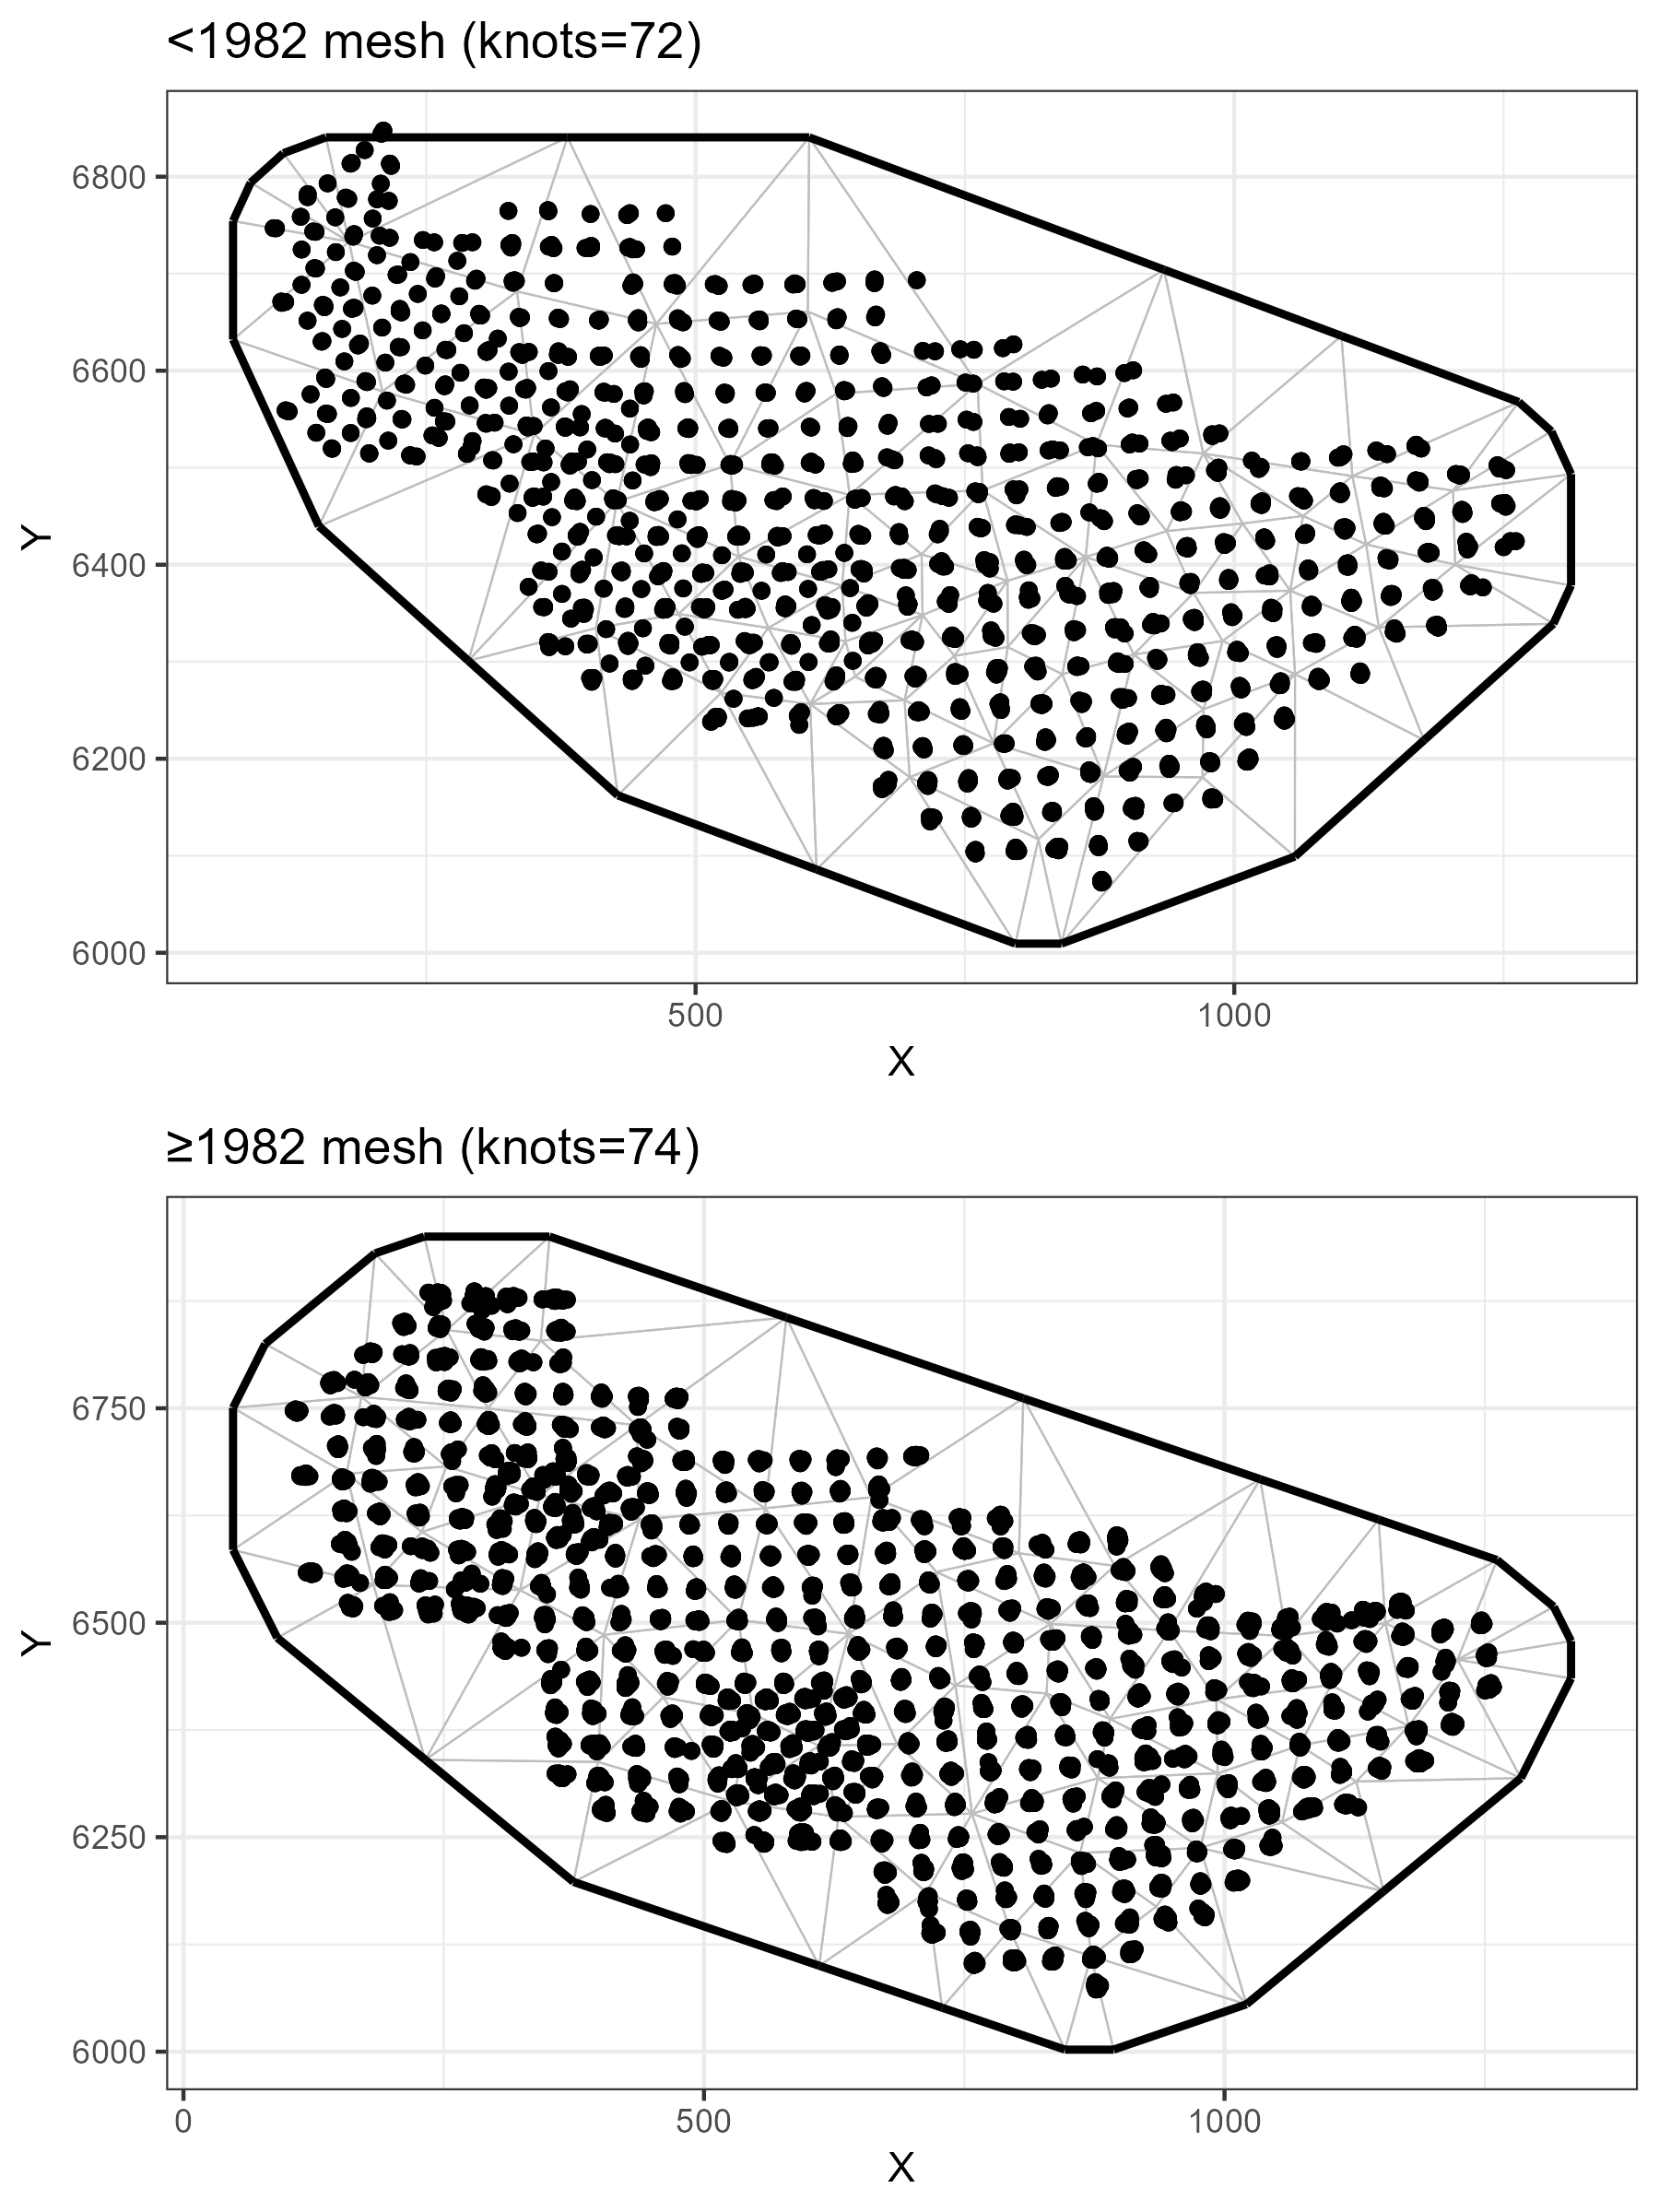
\includegraphics[width=6in]{../BAIRDI/Figures/mesh50} 

}

\caption{Spatial mesh with 50 knots used for fitting Tanner crab spatial models. Points represent observations and vertices represent knot locations. The title denotes the realized number of knots after mesh generation. }\label{fig:bairdi-50-mesh}
\end{figure}

\begin{figure}

{\centering 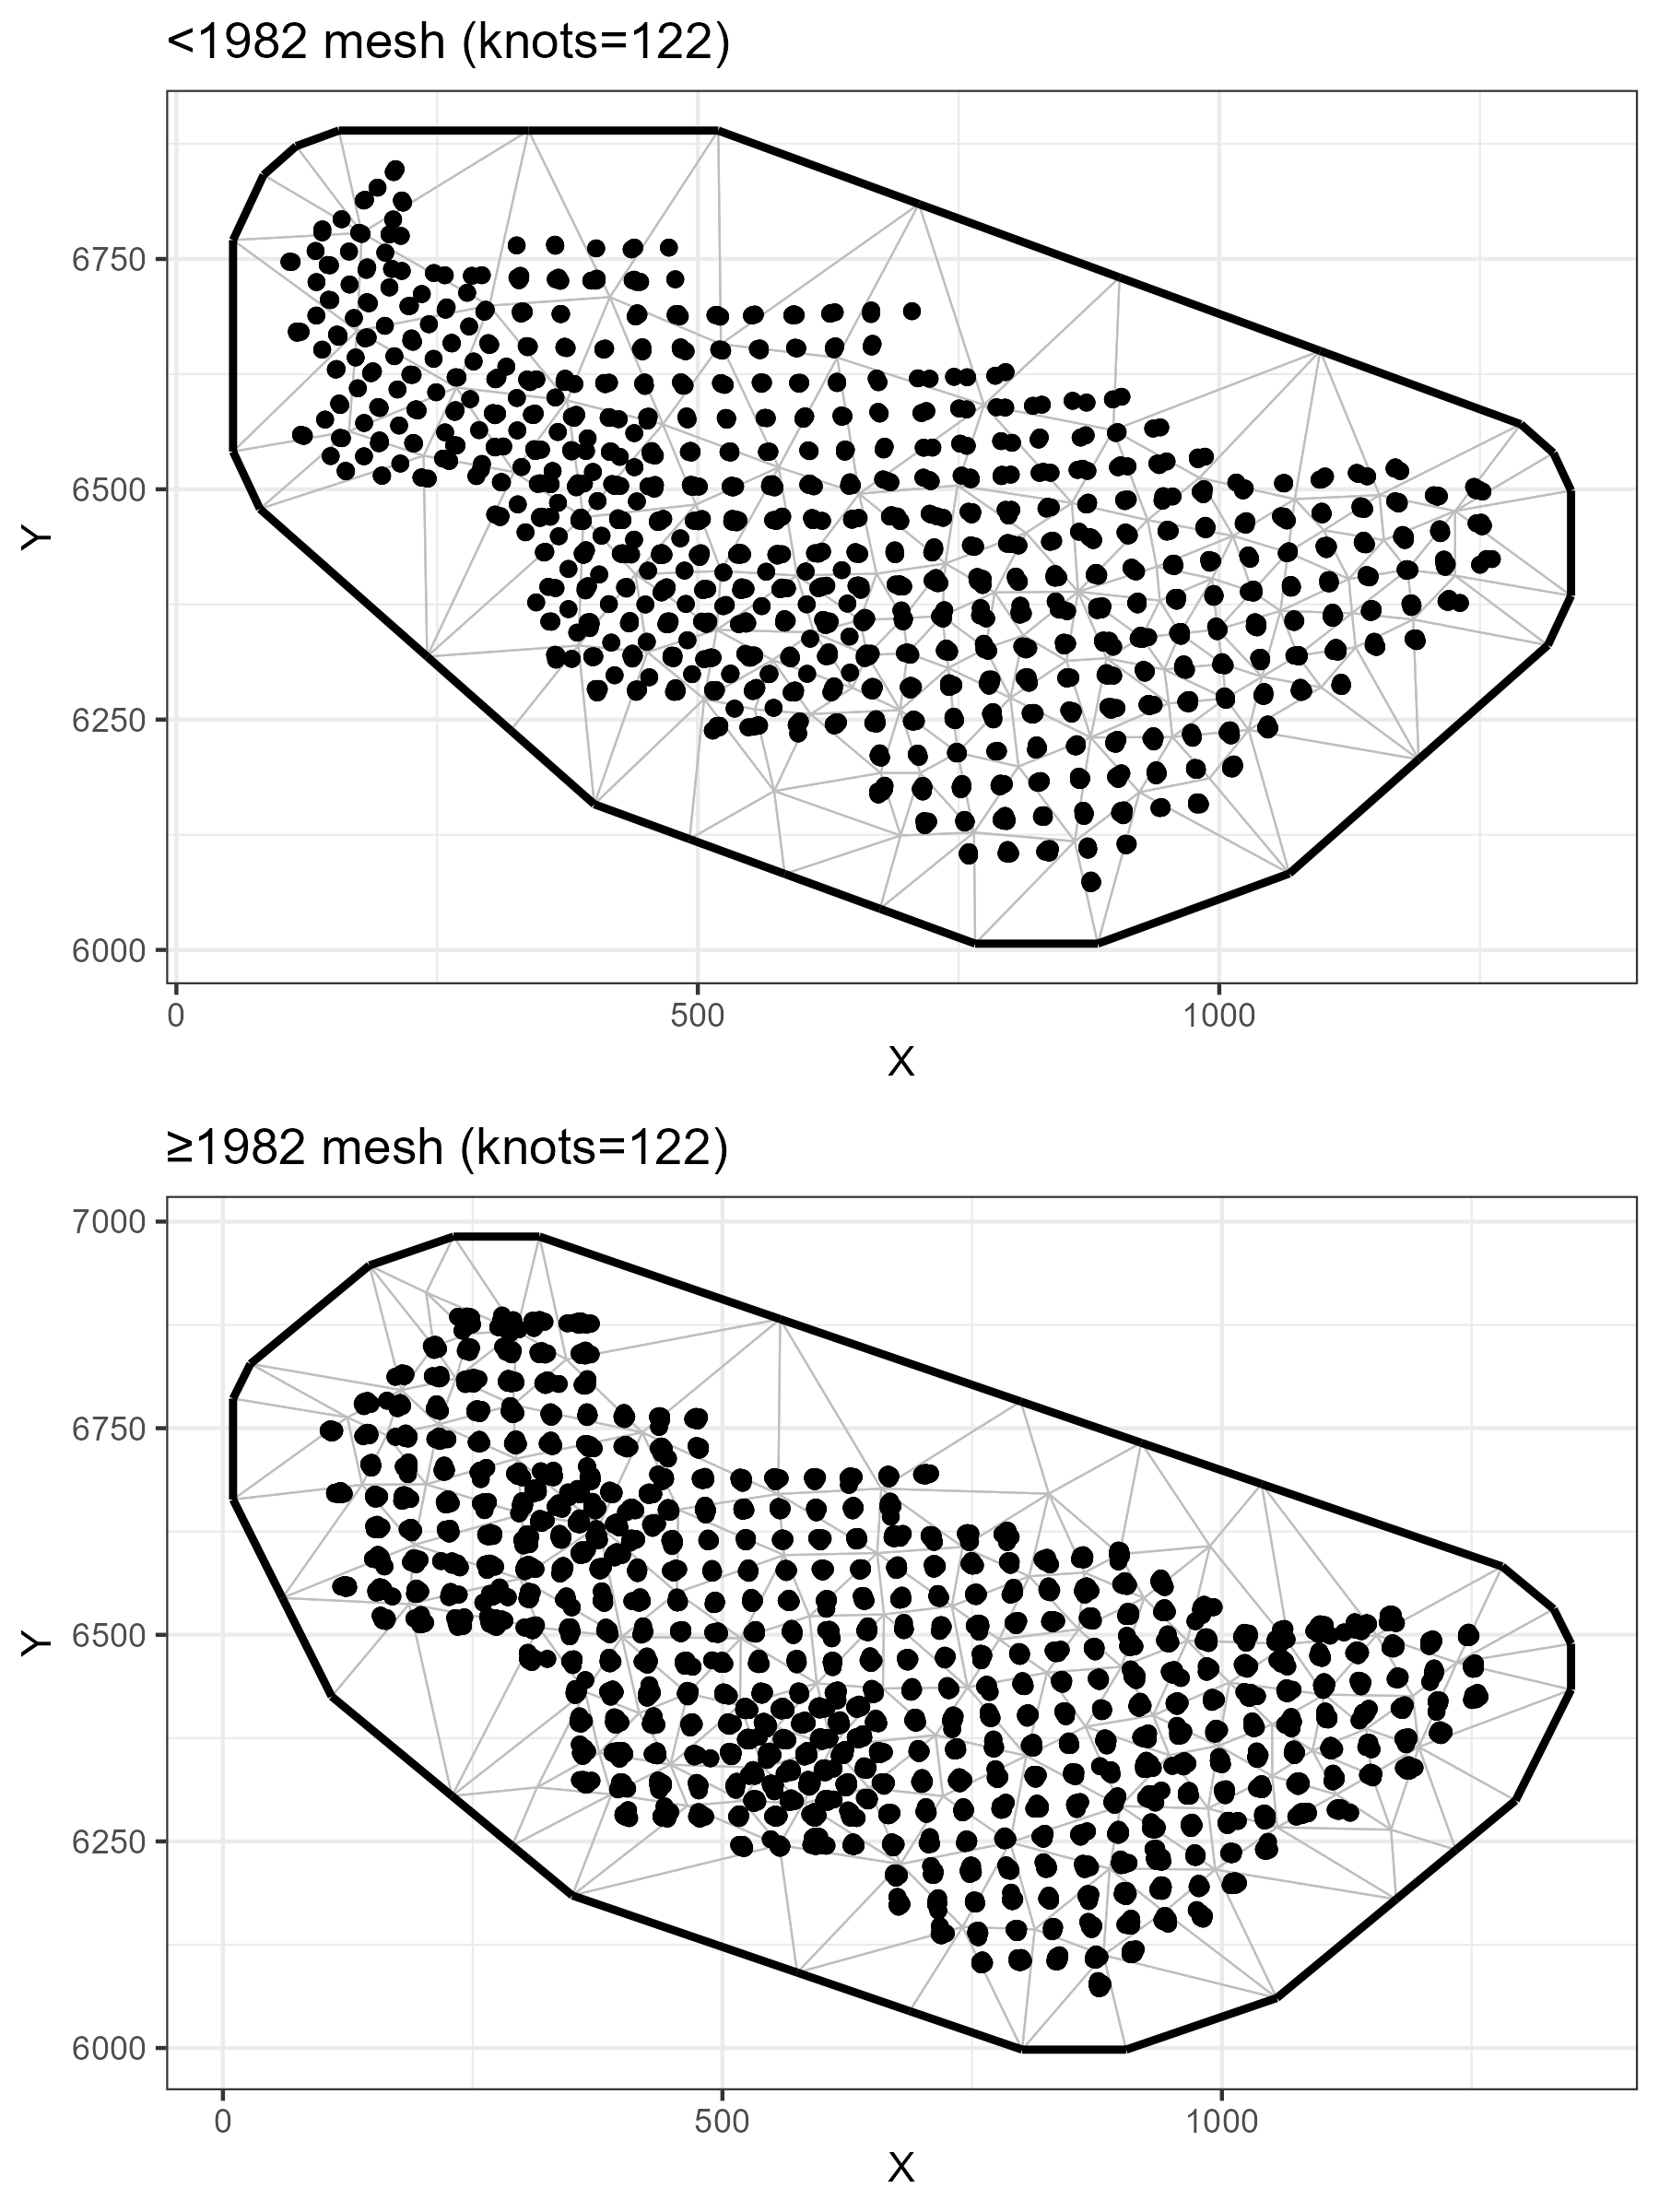
\includegraphics[width=6in]{../BAIRDI/Figures/mesh90} 

}

\caption{Spatial mesh with 90 knots used for fitting Tanner crab spatial models. Points represent observations and vertices represent knot locations. The title denotes the realized number of knots after mesh generation. }\label{fig:bairdi-90-mesh}
\end{figure}

\begin{figure}

{\centering 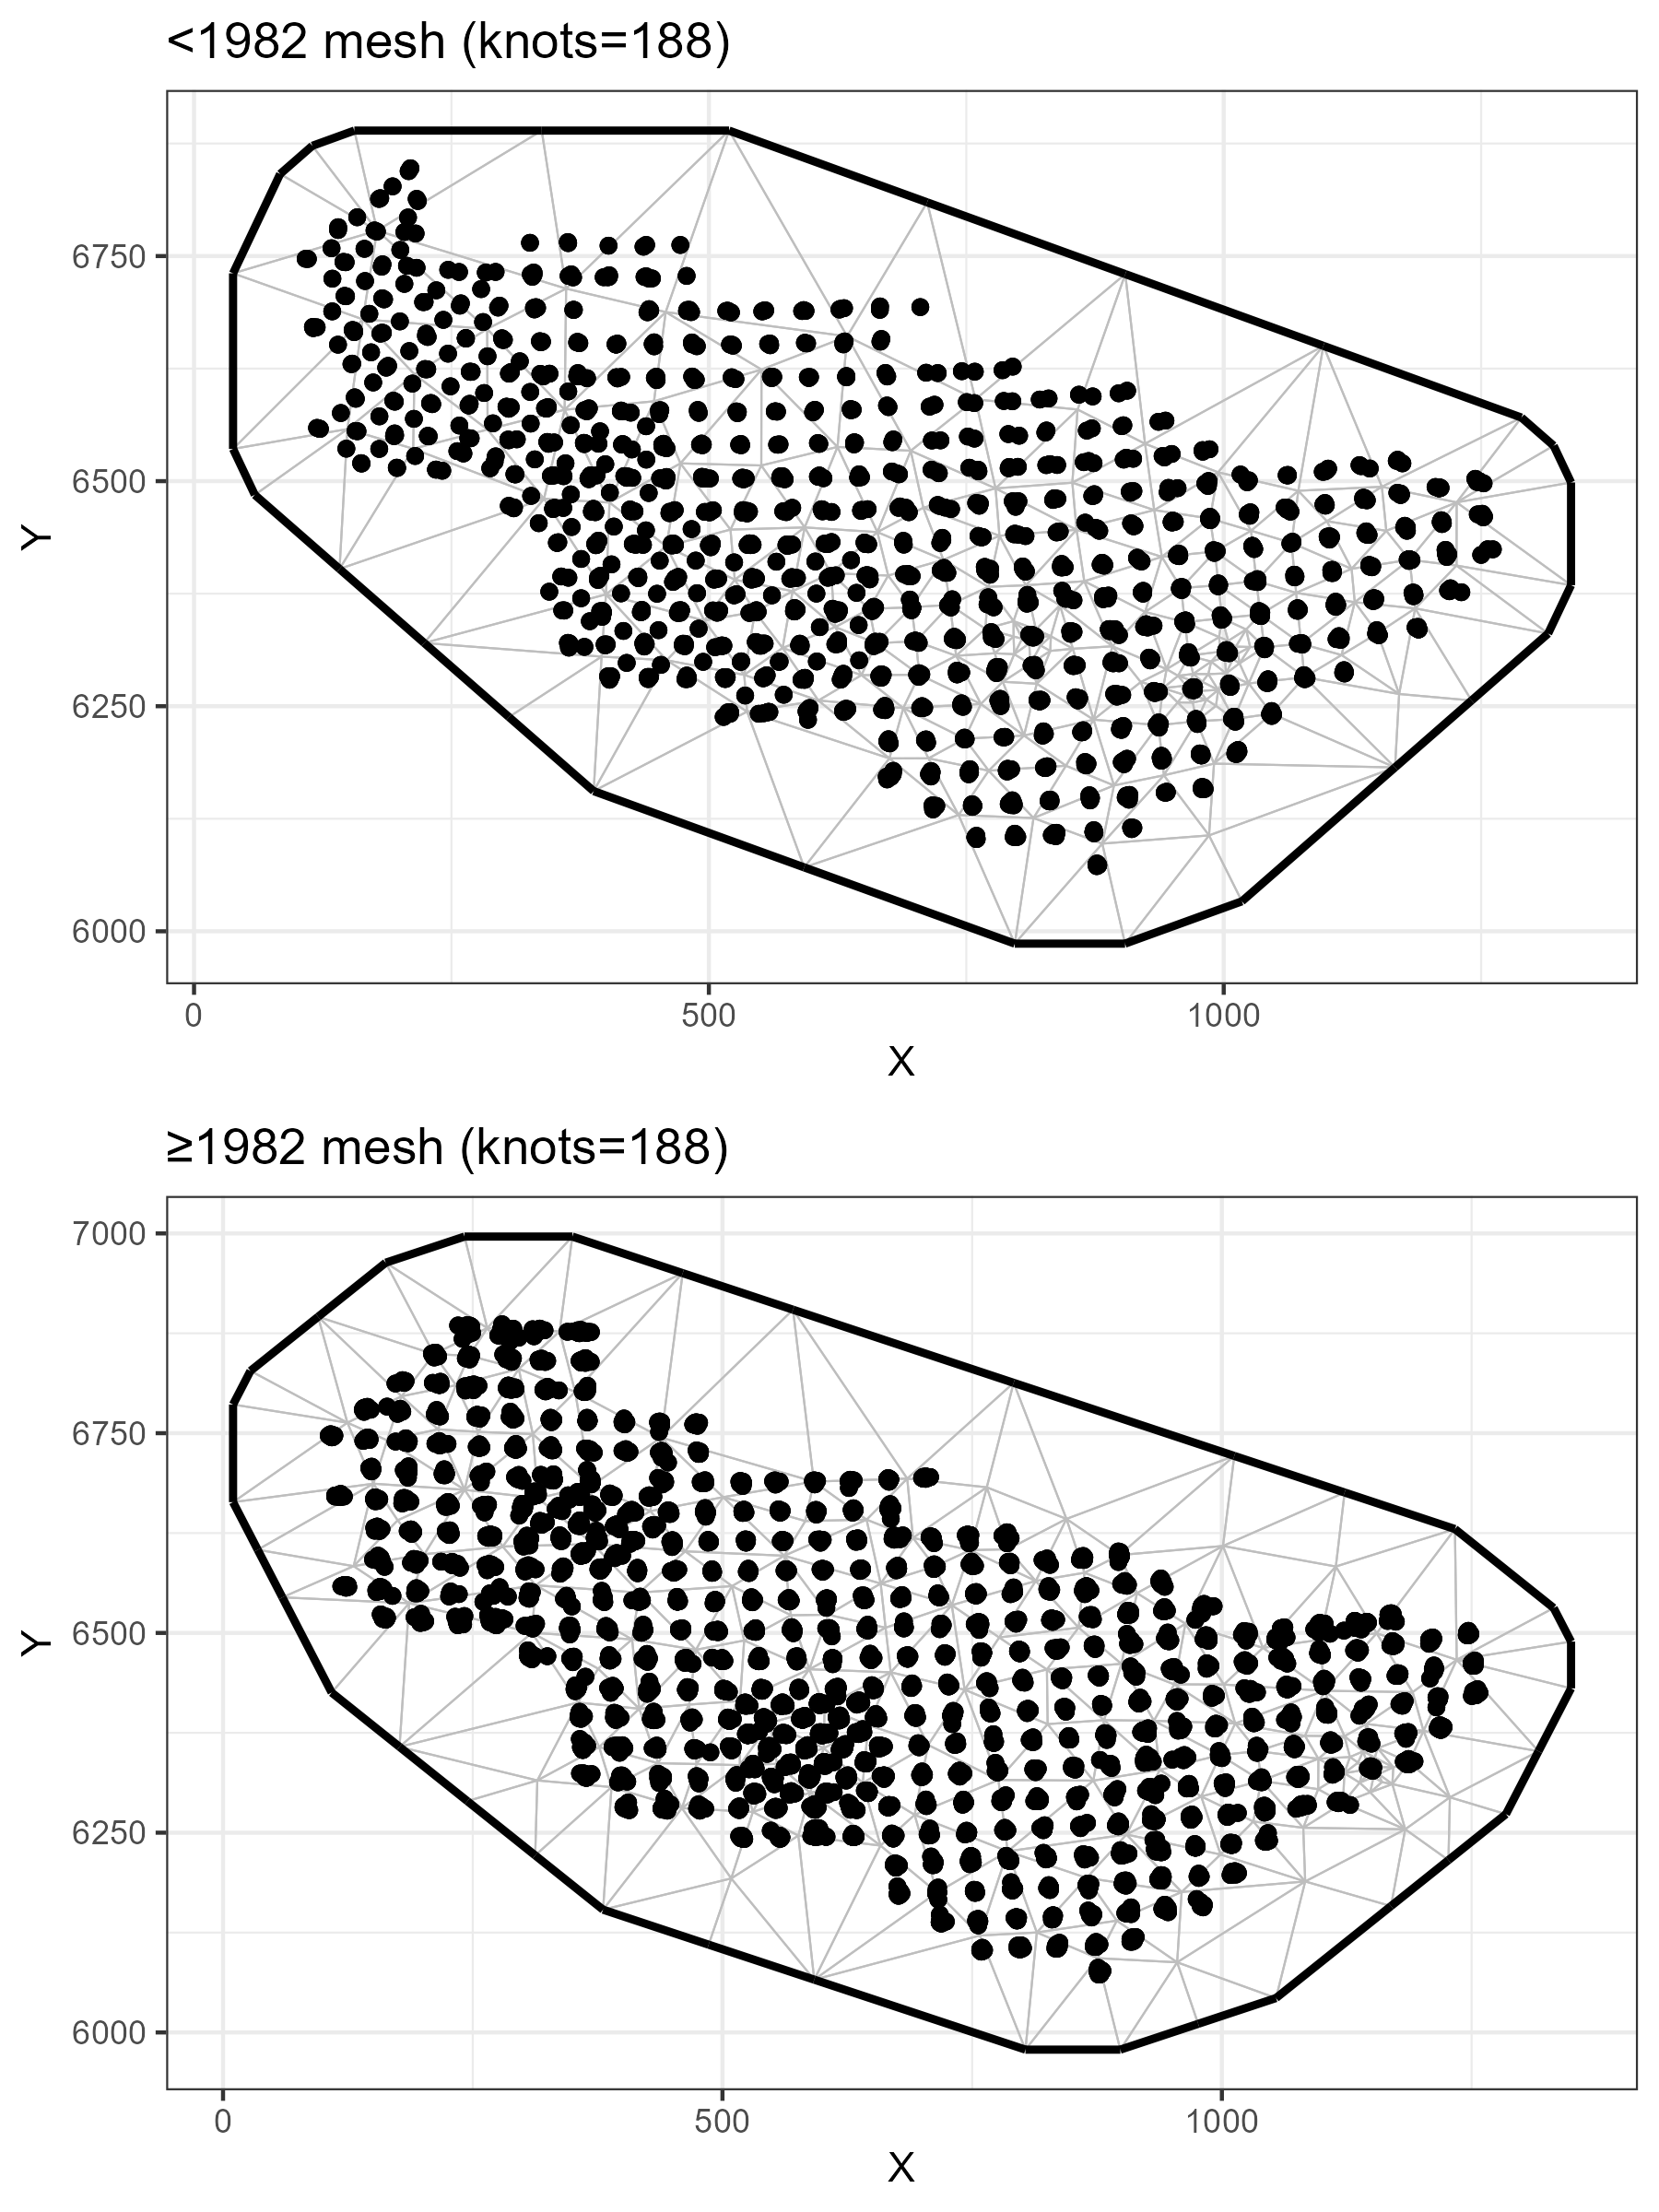
\includegraphics[width=6in]{../BAIRDI/Figures/mesh120} 

}

\caption{Spatial mesh with 120 knots used for fitting Tanner crab spatial models. Points represent observations and vertices represent knot locations. The title denotes the realized number of knots after mesh generation. }\label{fig:bairdi-120-mesh}
\end{figure}

\begin{figure}

{\centering 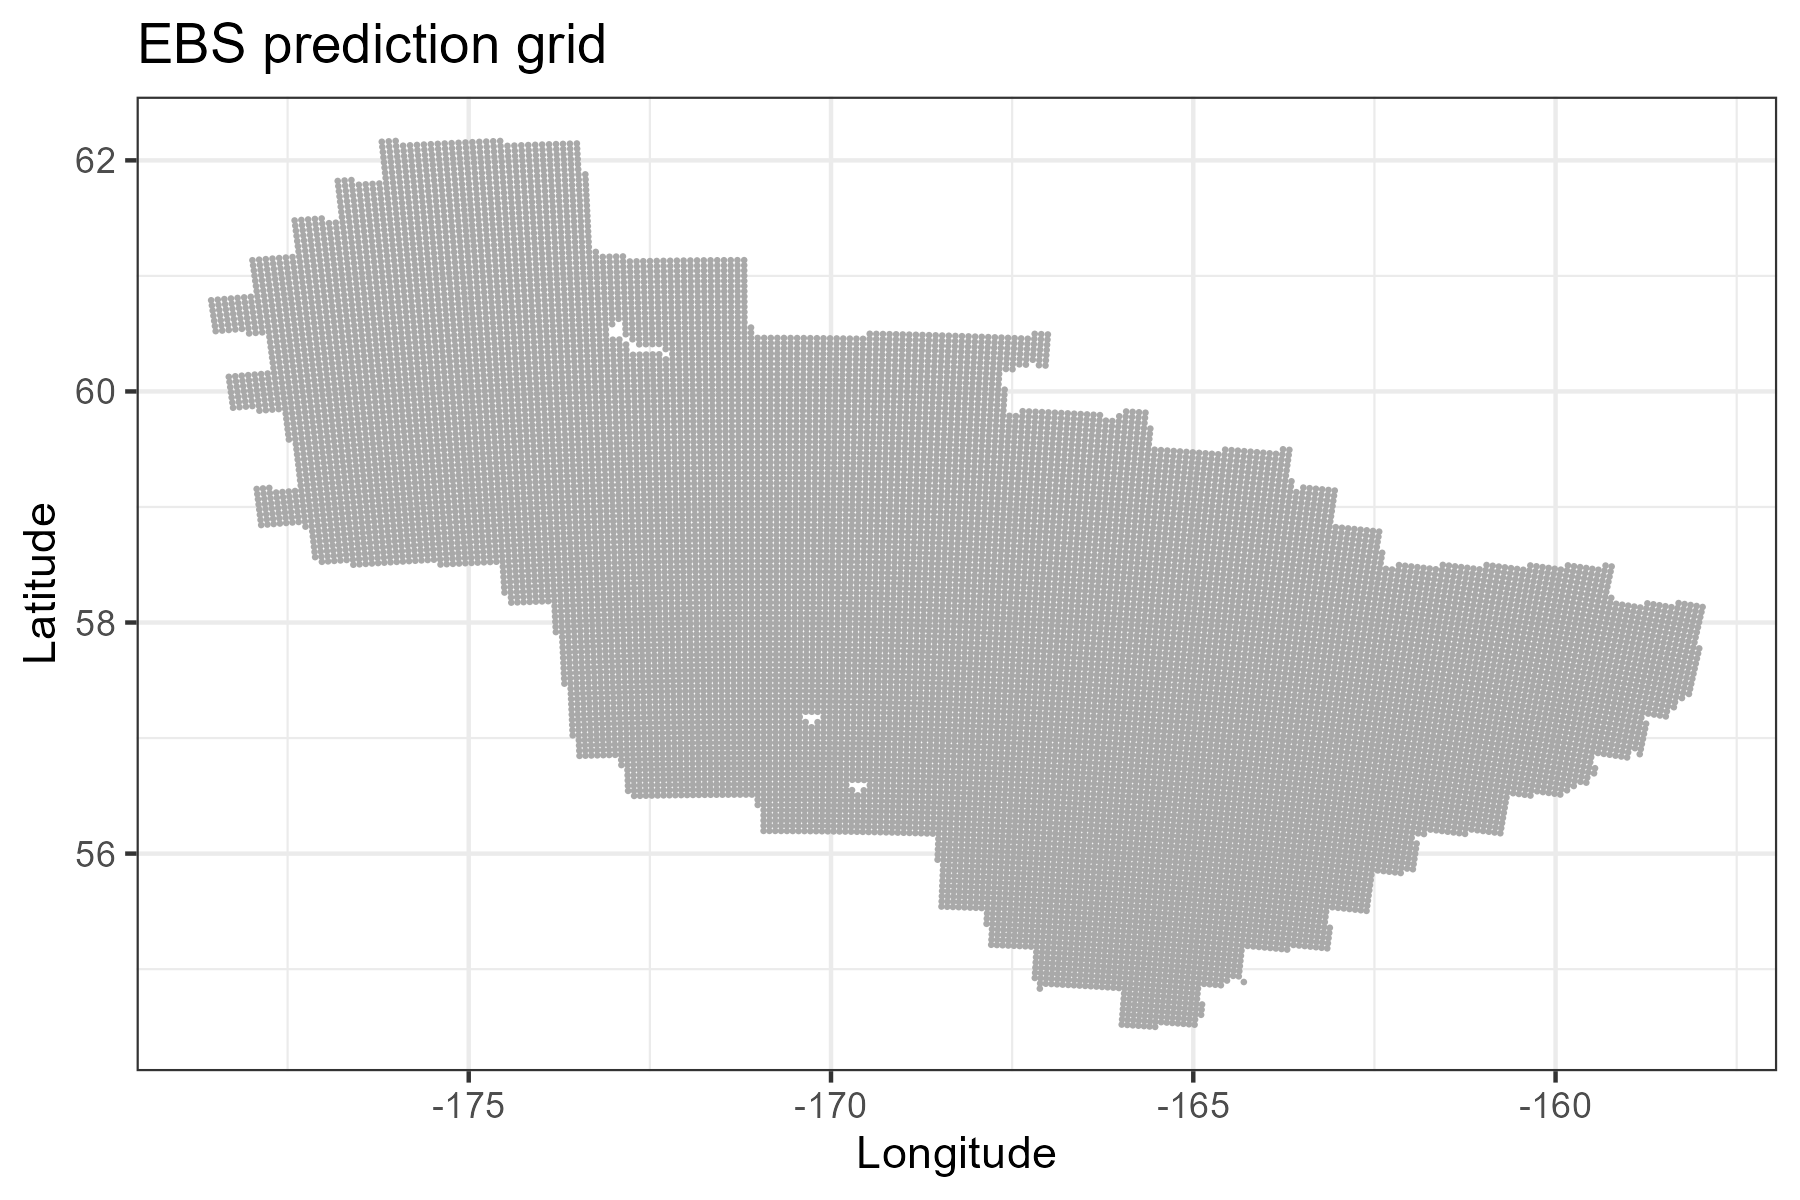
\includegraphics[width=6in]{../BAIRDI/Figures/EBS_predgrid} 

}

\caption{Eastern Bering Sea prediction grid used for Tanner crab spatial abundance and biomass predictions. Spatial resolution is 5km$^2$ and does not include land.}\label{fig:bairdi-EBS-grid}
\end{figure}

\begin{figure}

{\centering 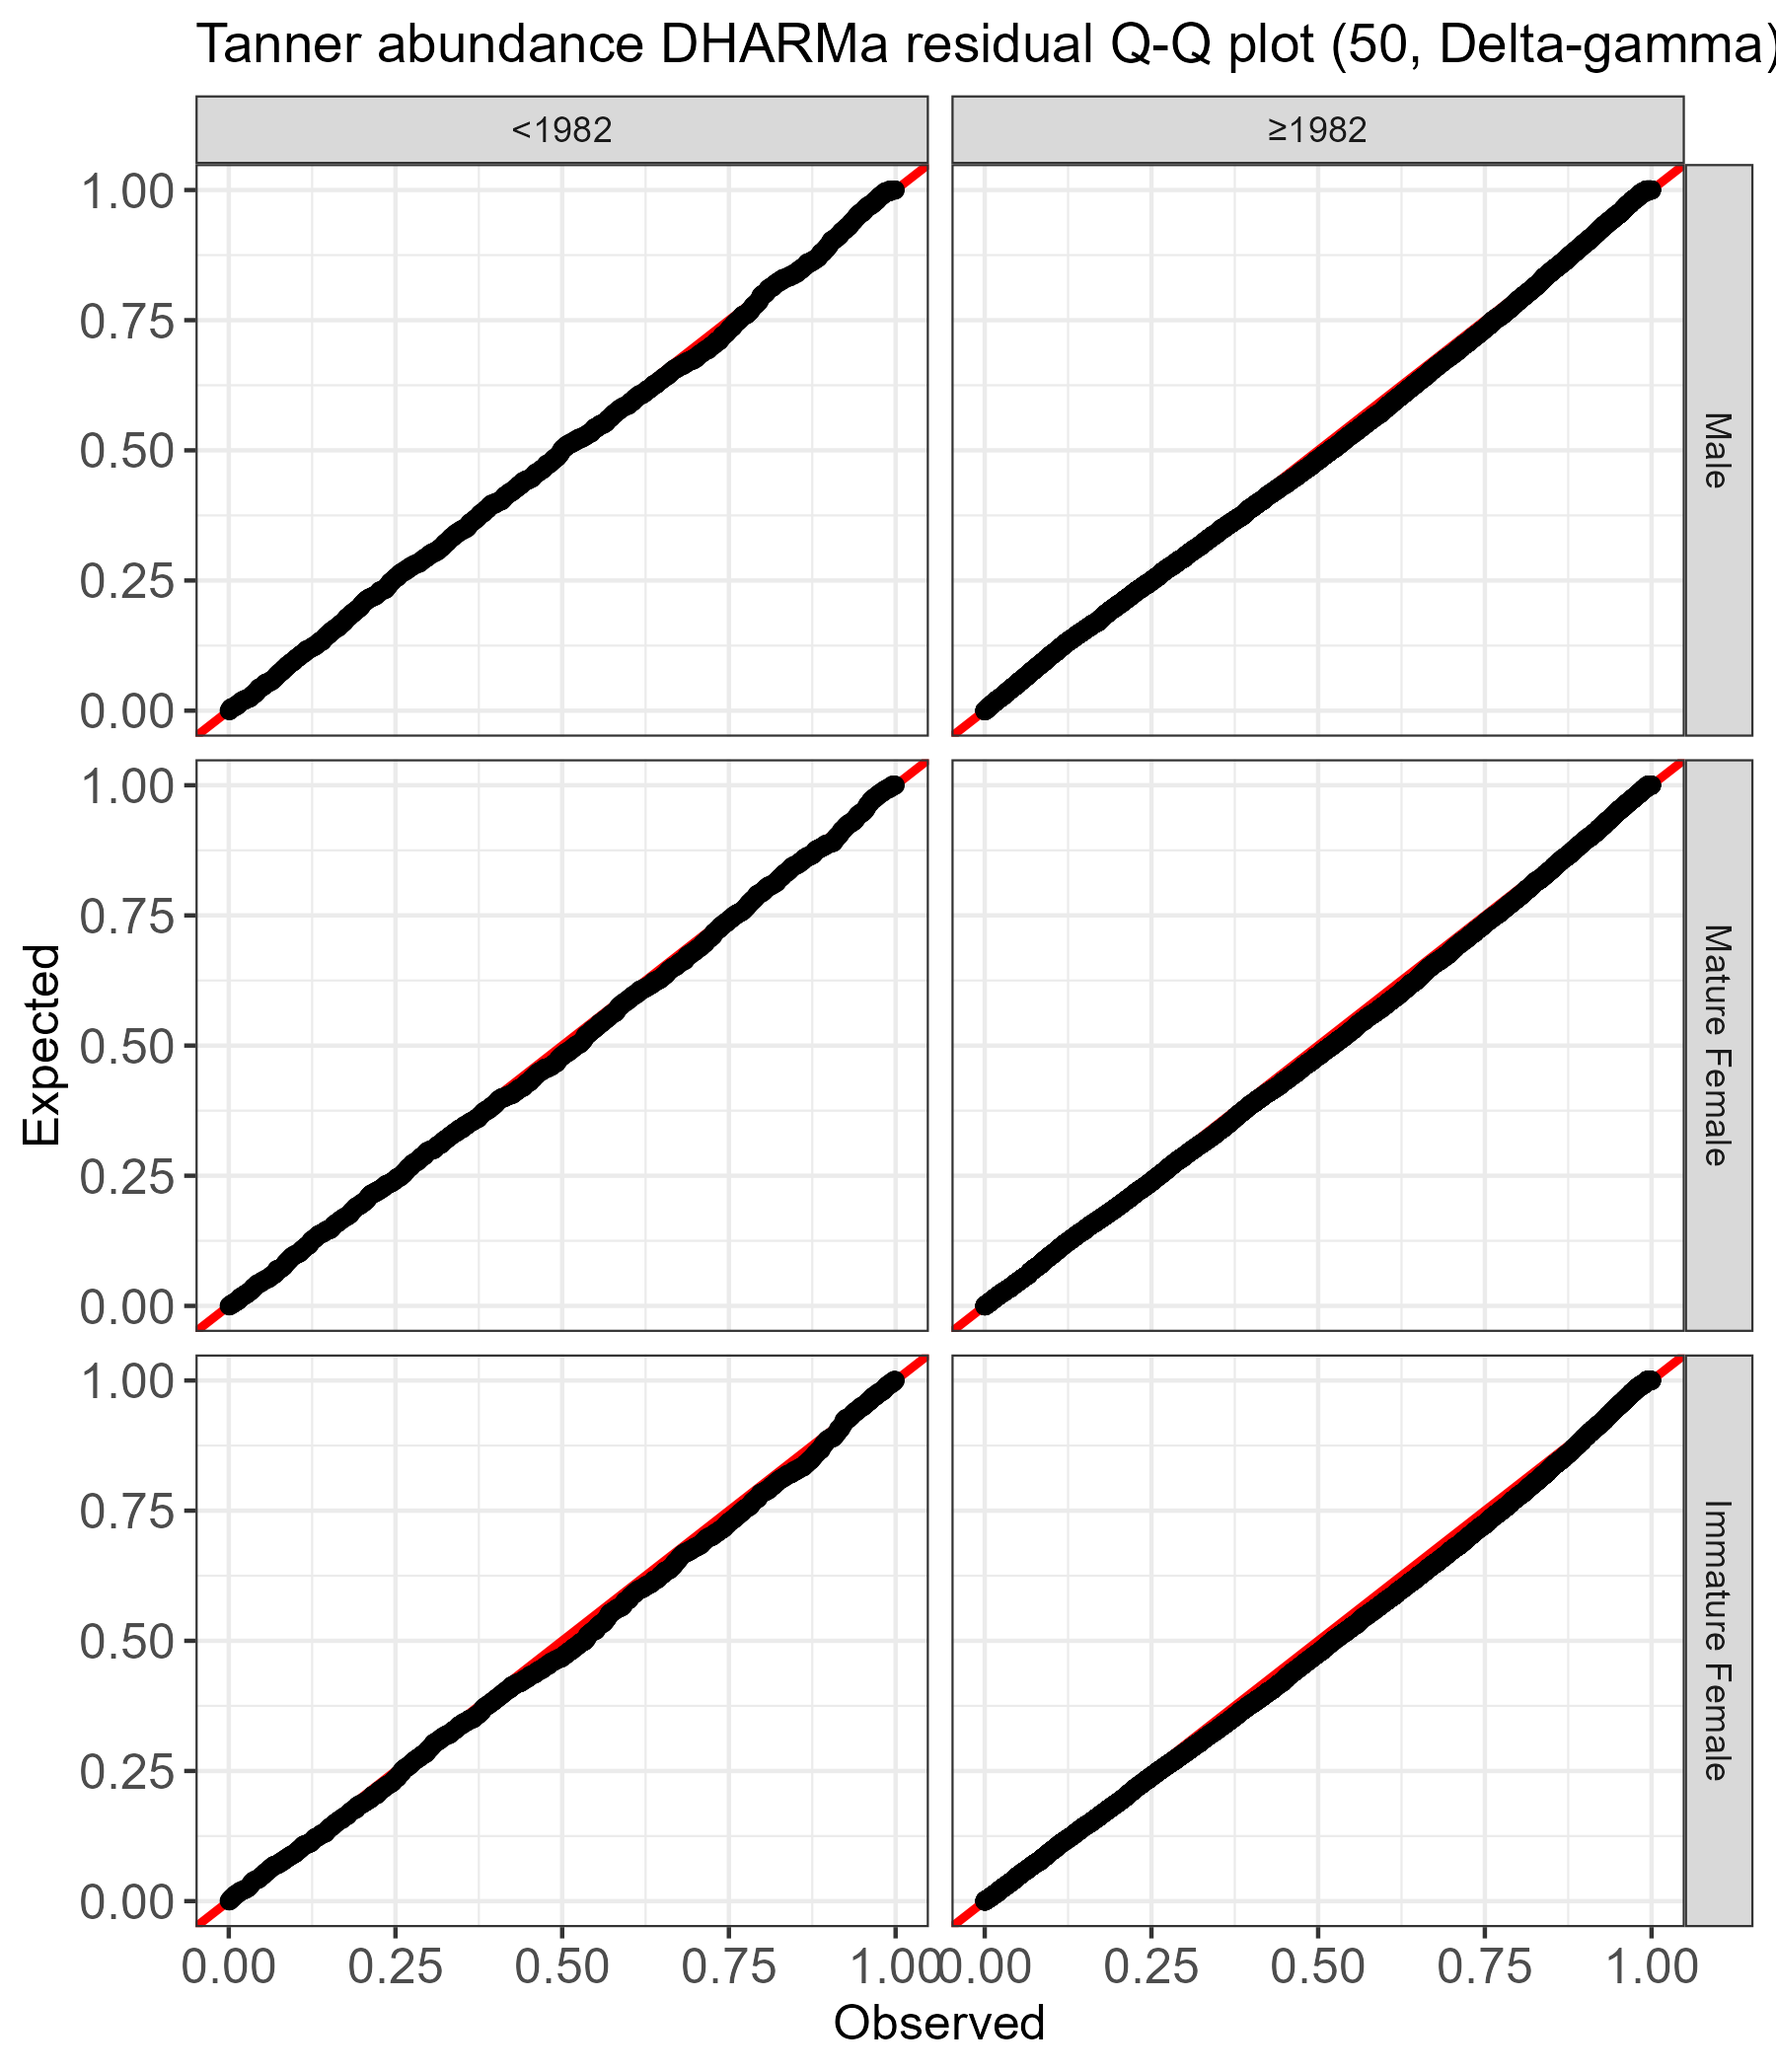
\includegraphics[width=6in]{../BAIRDI/Figures/DHARMa_abundance_50-Delta-gamma_QQplot} 

}

\caption{Q-Q plot of DHARMa residuals for abundance models fit with NMFS summer bottom trawl survey data before 1982 (left) and 1982 onward (right) using a delta-gamma model family and 50 knots in the model mesh.}\label{fig:DHARMa-abund-QQ-50}
\end{figure}

\begin{figure}

{\centering 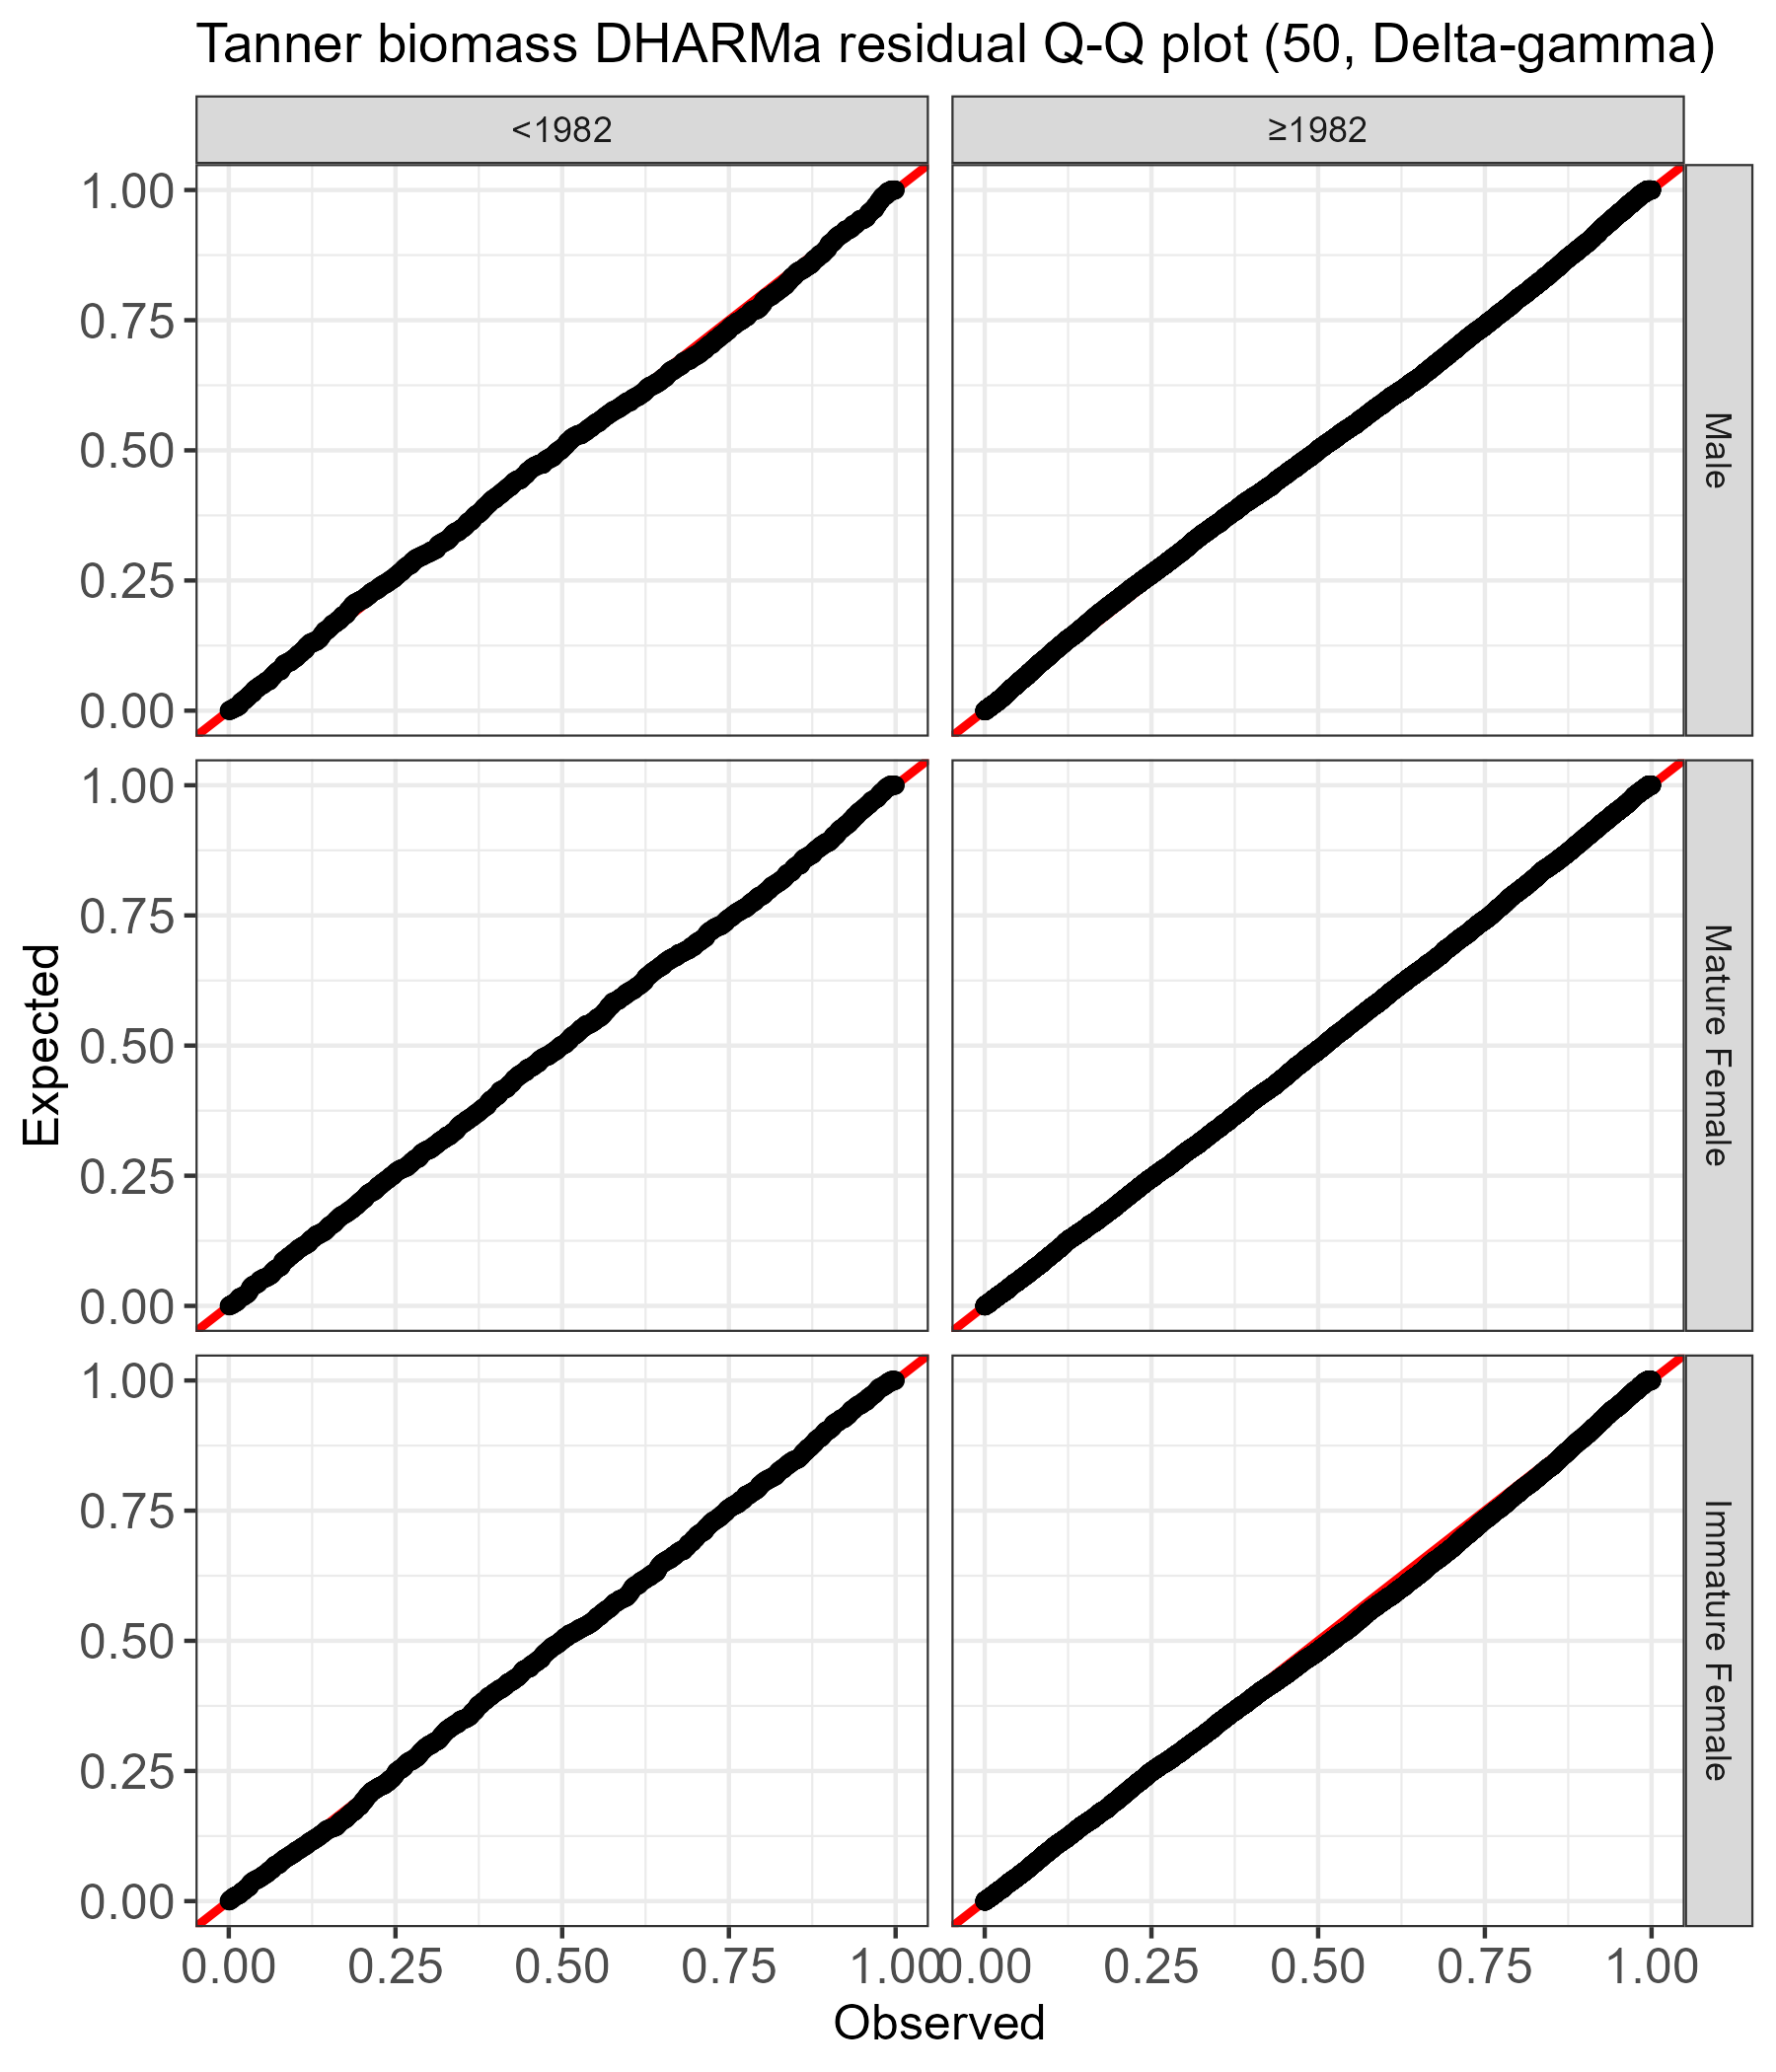
\includegraphics[width=6in]{../BAIRDI/Figures/DHARMa_biomass_50-Delta-gamma_QQplot} 

}

\caption{Q-Q plot of DHARMa residuals for biomass models fit with NMFS summer bottom trawl survey data before 1982 (left) and 1982 onward (right) using a delta-gamma model family and 50 knots in the model mesh.}\label{fig:DHARMa-bio-QQ-50}
\end{figure}

\begin{figure}

{\centering 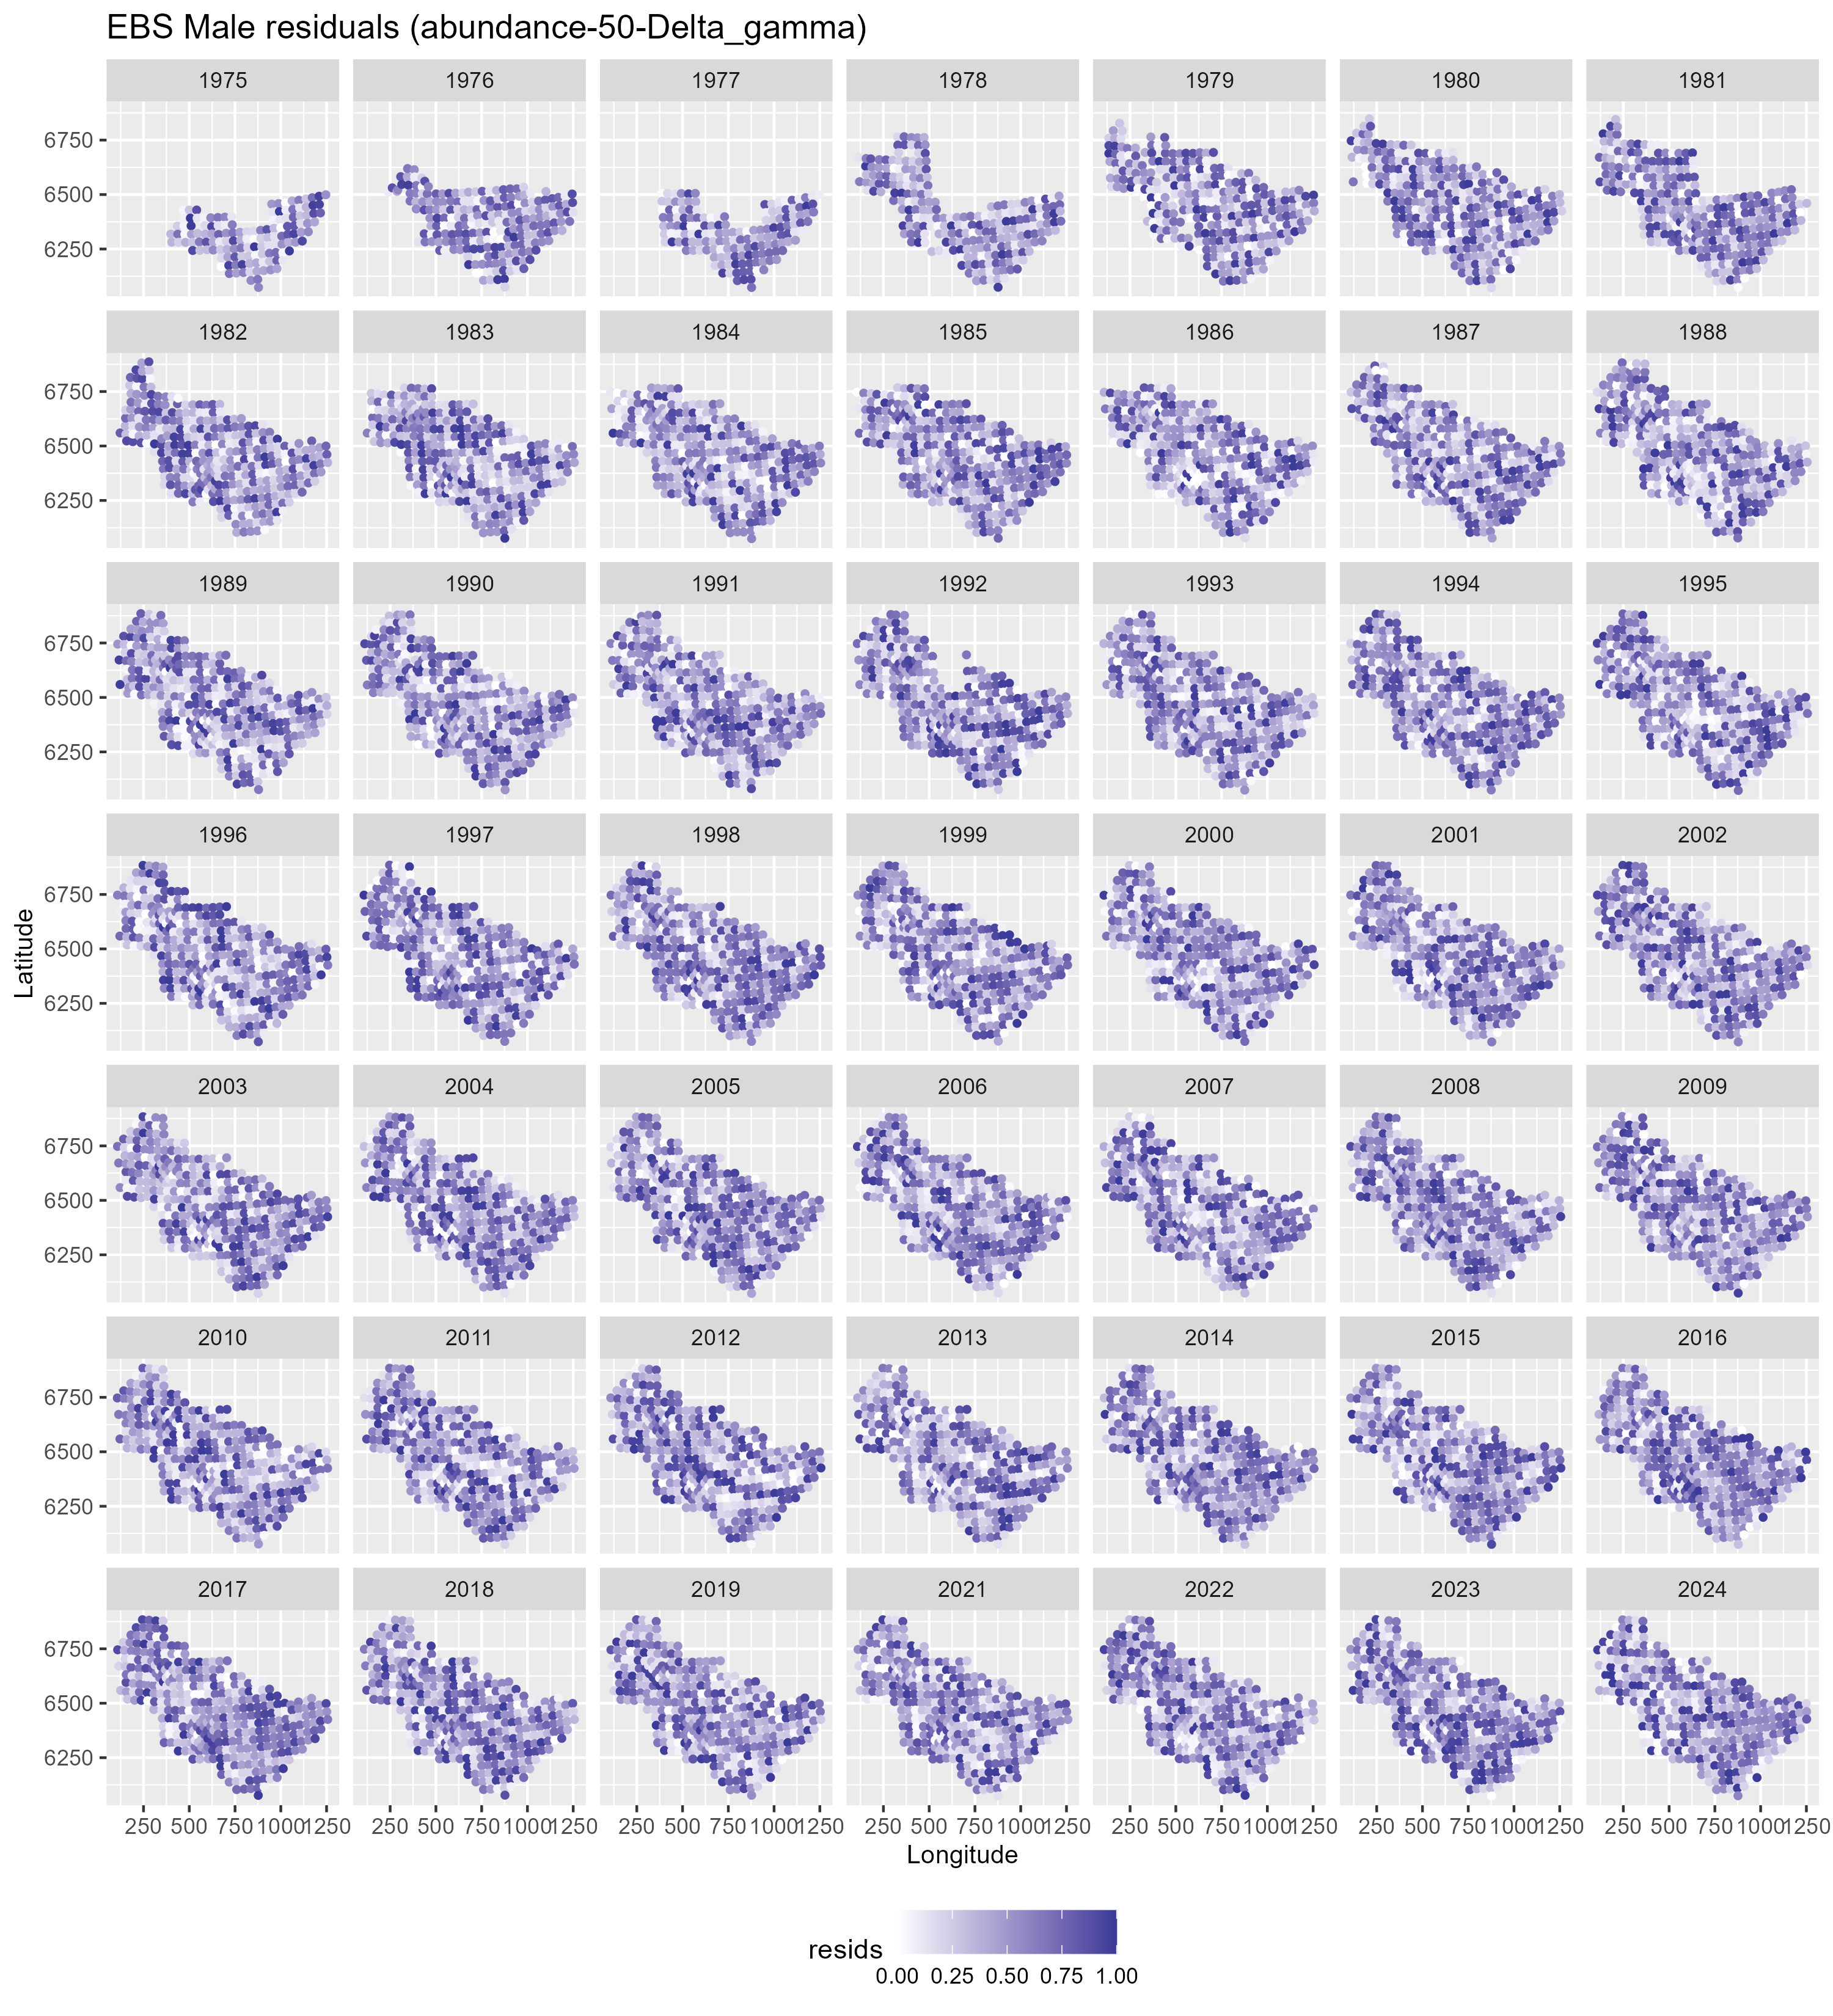
\includegraphics[width=1\linewidth,height=1\textheight]{../BAIRDI/Figures/DHARMa_Male_abundance-50-Delta_gamma_SPATIAL} 

}

\caption{Spatial plot of DHARMa residuals for male abundance models fit using NMFS summer bottom trawl survey data before 1982 and 1982 onward with a 50-knot mesh and a delta-gamma model family. Predictions from both of these periods/models are combined in this figure.}\label{fig:DHARMa-abund-spat-50-male}
\end{figure}

\begin{figure}

{\centering 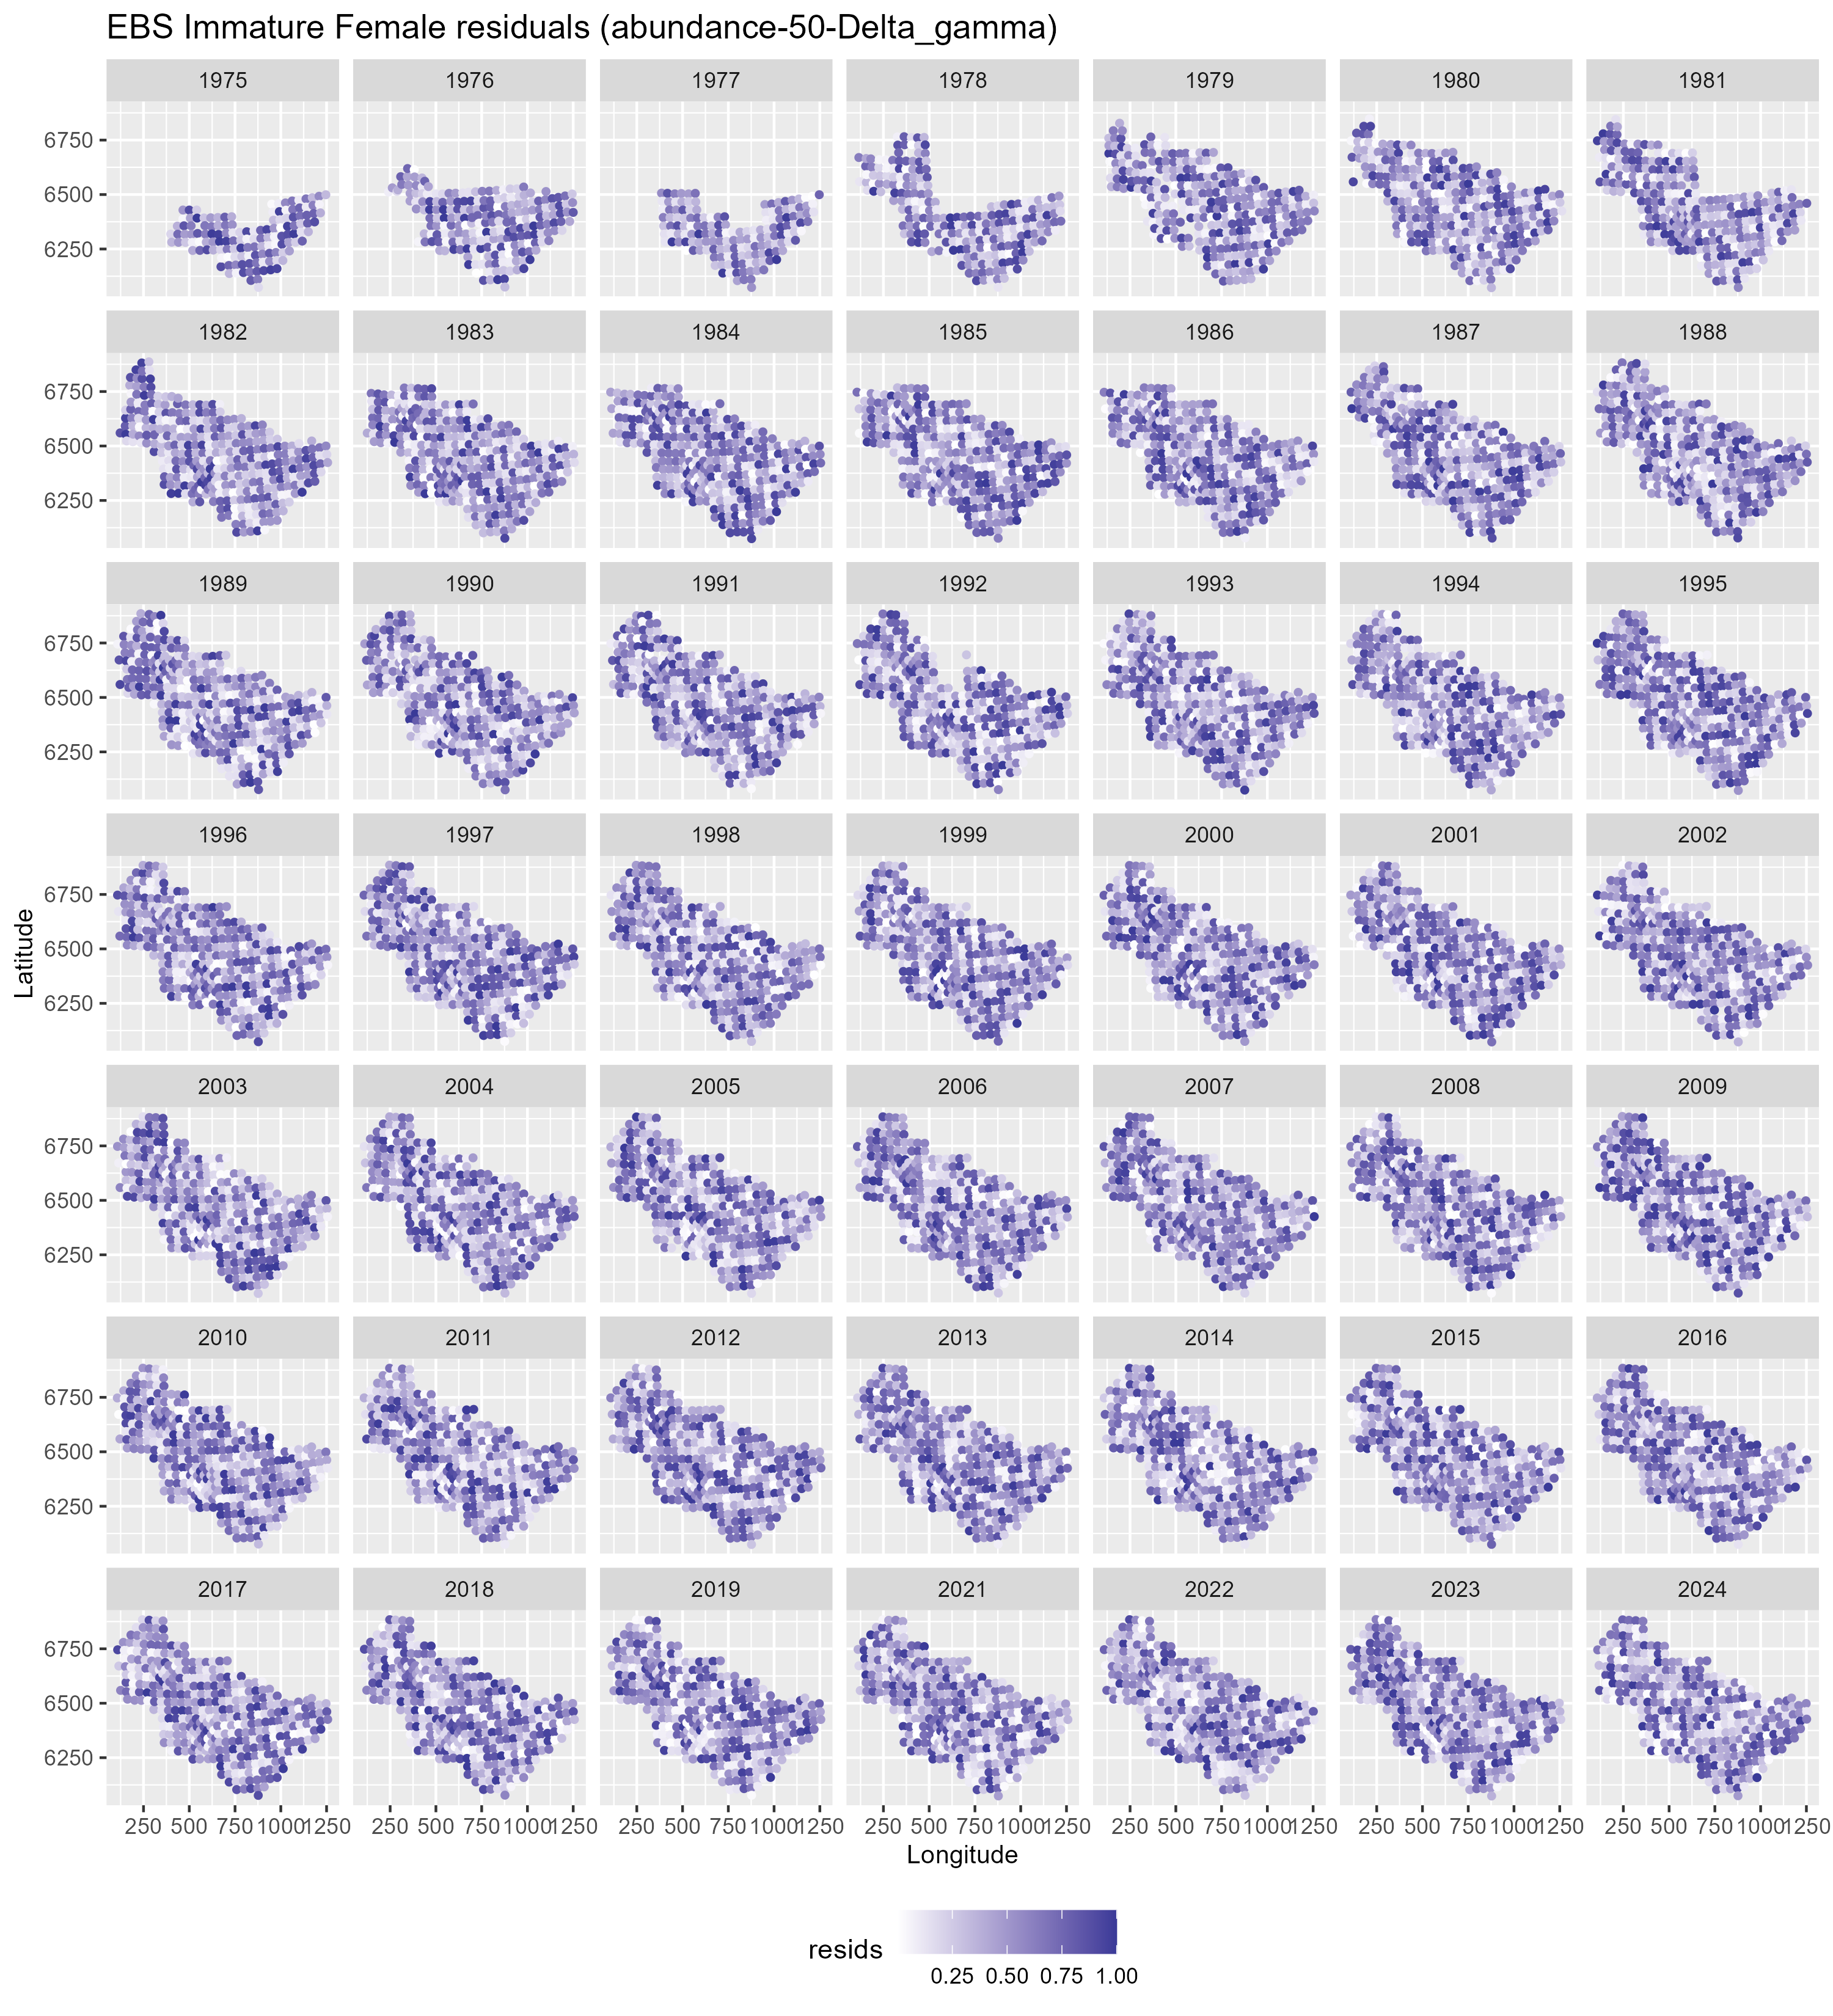
\includegraphics[width=1\linewidth,height=1\textheight]{../BAIRDI/Figures/DHARMa_Immature Female_abundance-50-Delta_gamma_SPATIAL} 

}

\caption{Spatial plot of DHARMa residuals for immature female abundance models fit using NMFS summer bottom trawl survey data before 1982 and 1982 onward with a 50-knot mesh and a delta-gamma model family. Predictions from both of these periods/models are combined in this figure.}\label{fig:DHARMa-abund-spat-50-imfem}
\end{figure}

\begin{figure}

{\centering 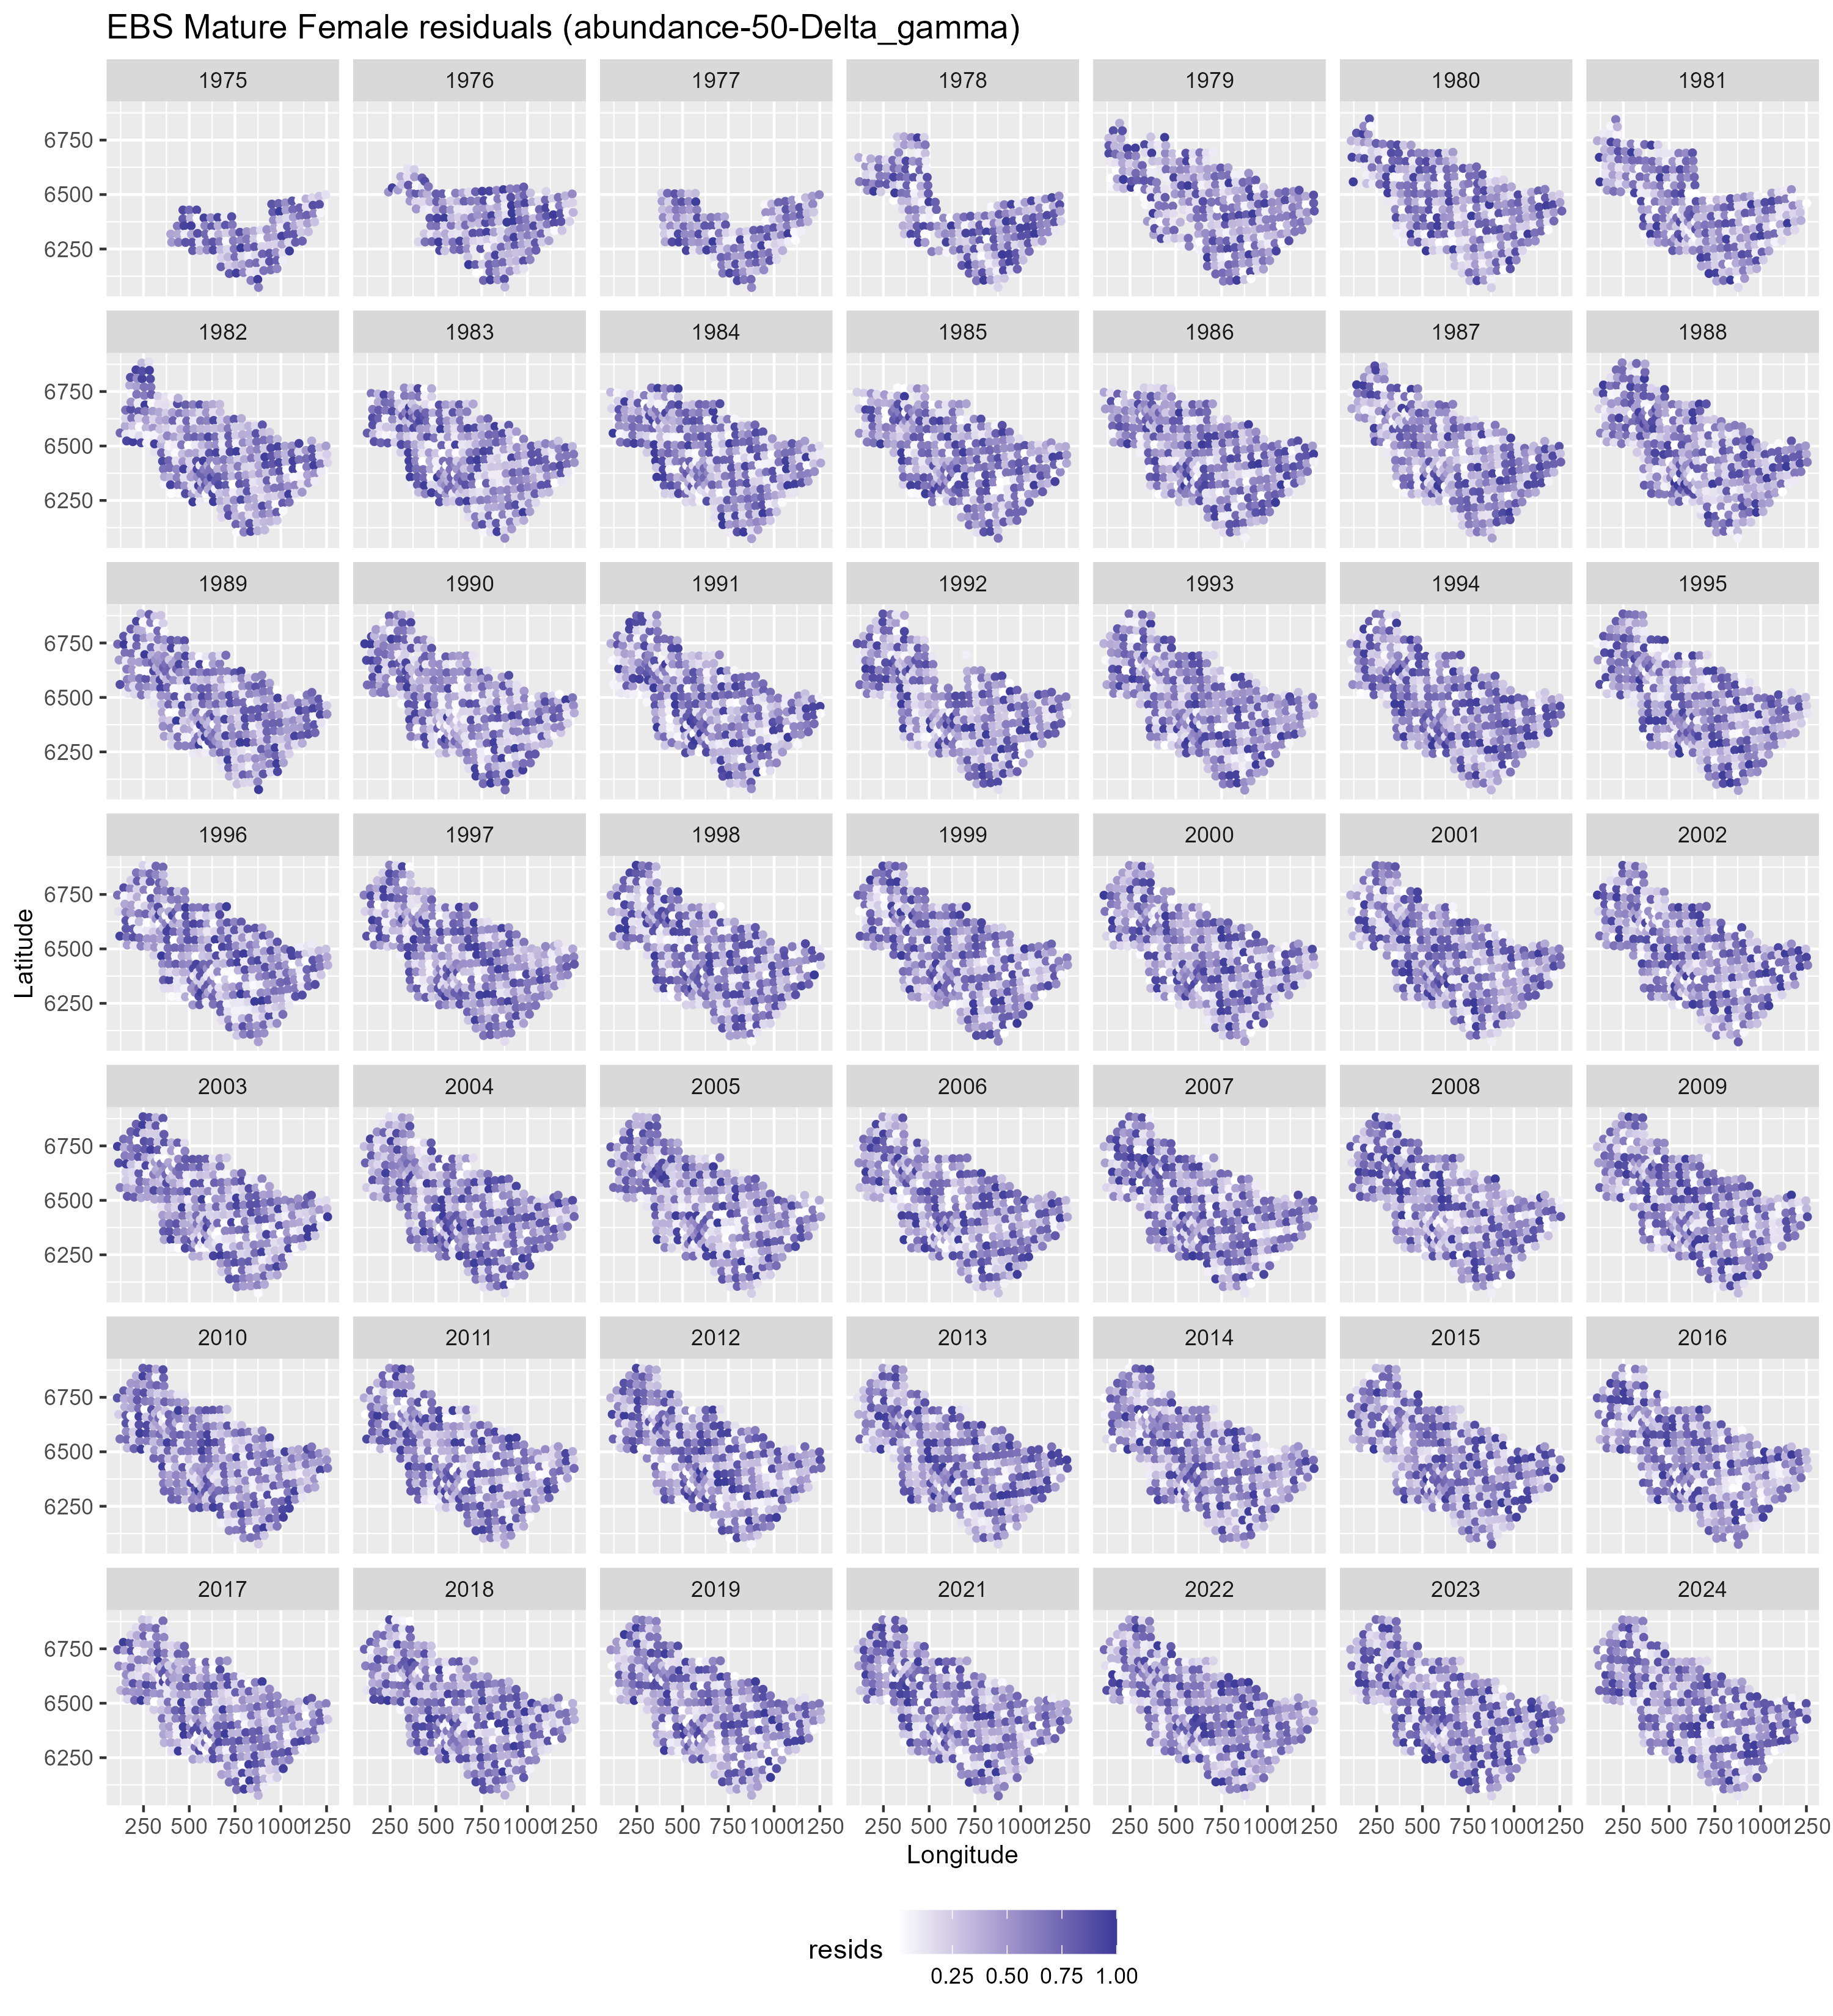
\includegraphics[width=1\linewidth,height=1\textheight]{../BAIRDI/Figures/DHARMa_Mature Female_abundance-50-Delta_gamma_SPATIAL} 

}

\caption{Spatial plot of DHARMa residuals for mature female abundance models fit using NMFS summer bottom trawl survey data before 1982 and 1982 onward with a 50-knot mesh and a delta-gamma model family. Predictions from both of these periods/models are combined in this figure.}\label{fig:DHARMa-abund-spat-50-matfem}
\end{figure}

\begin{figure}

{\centering 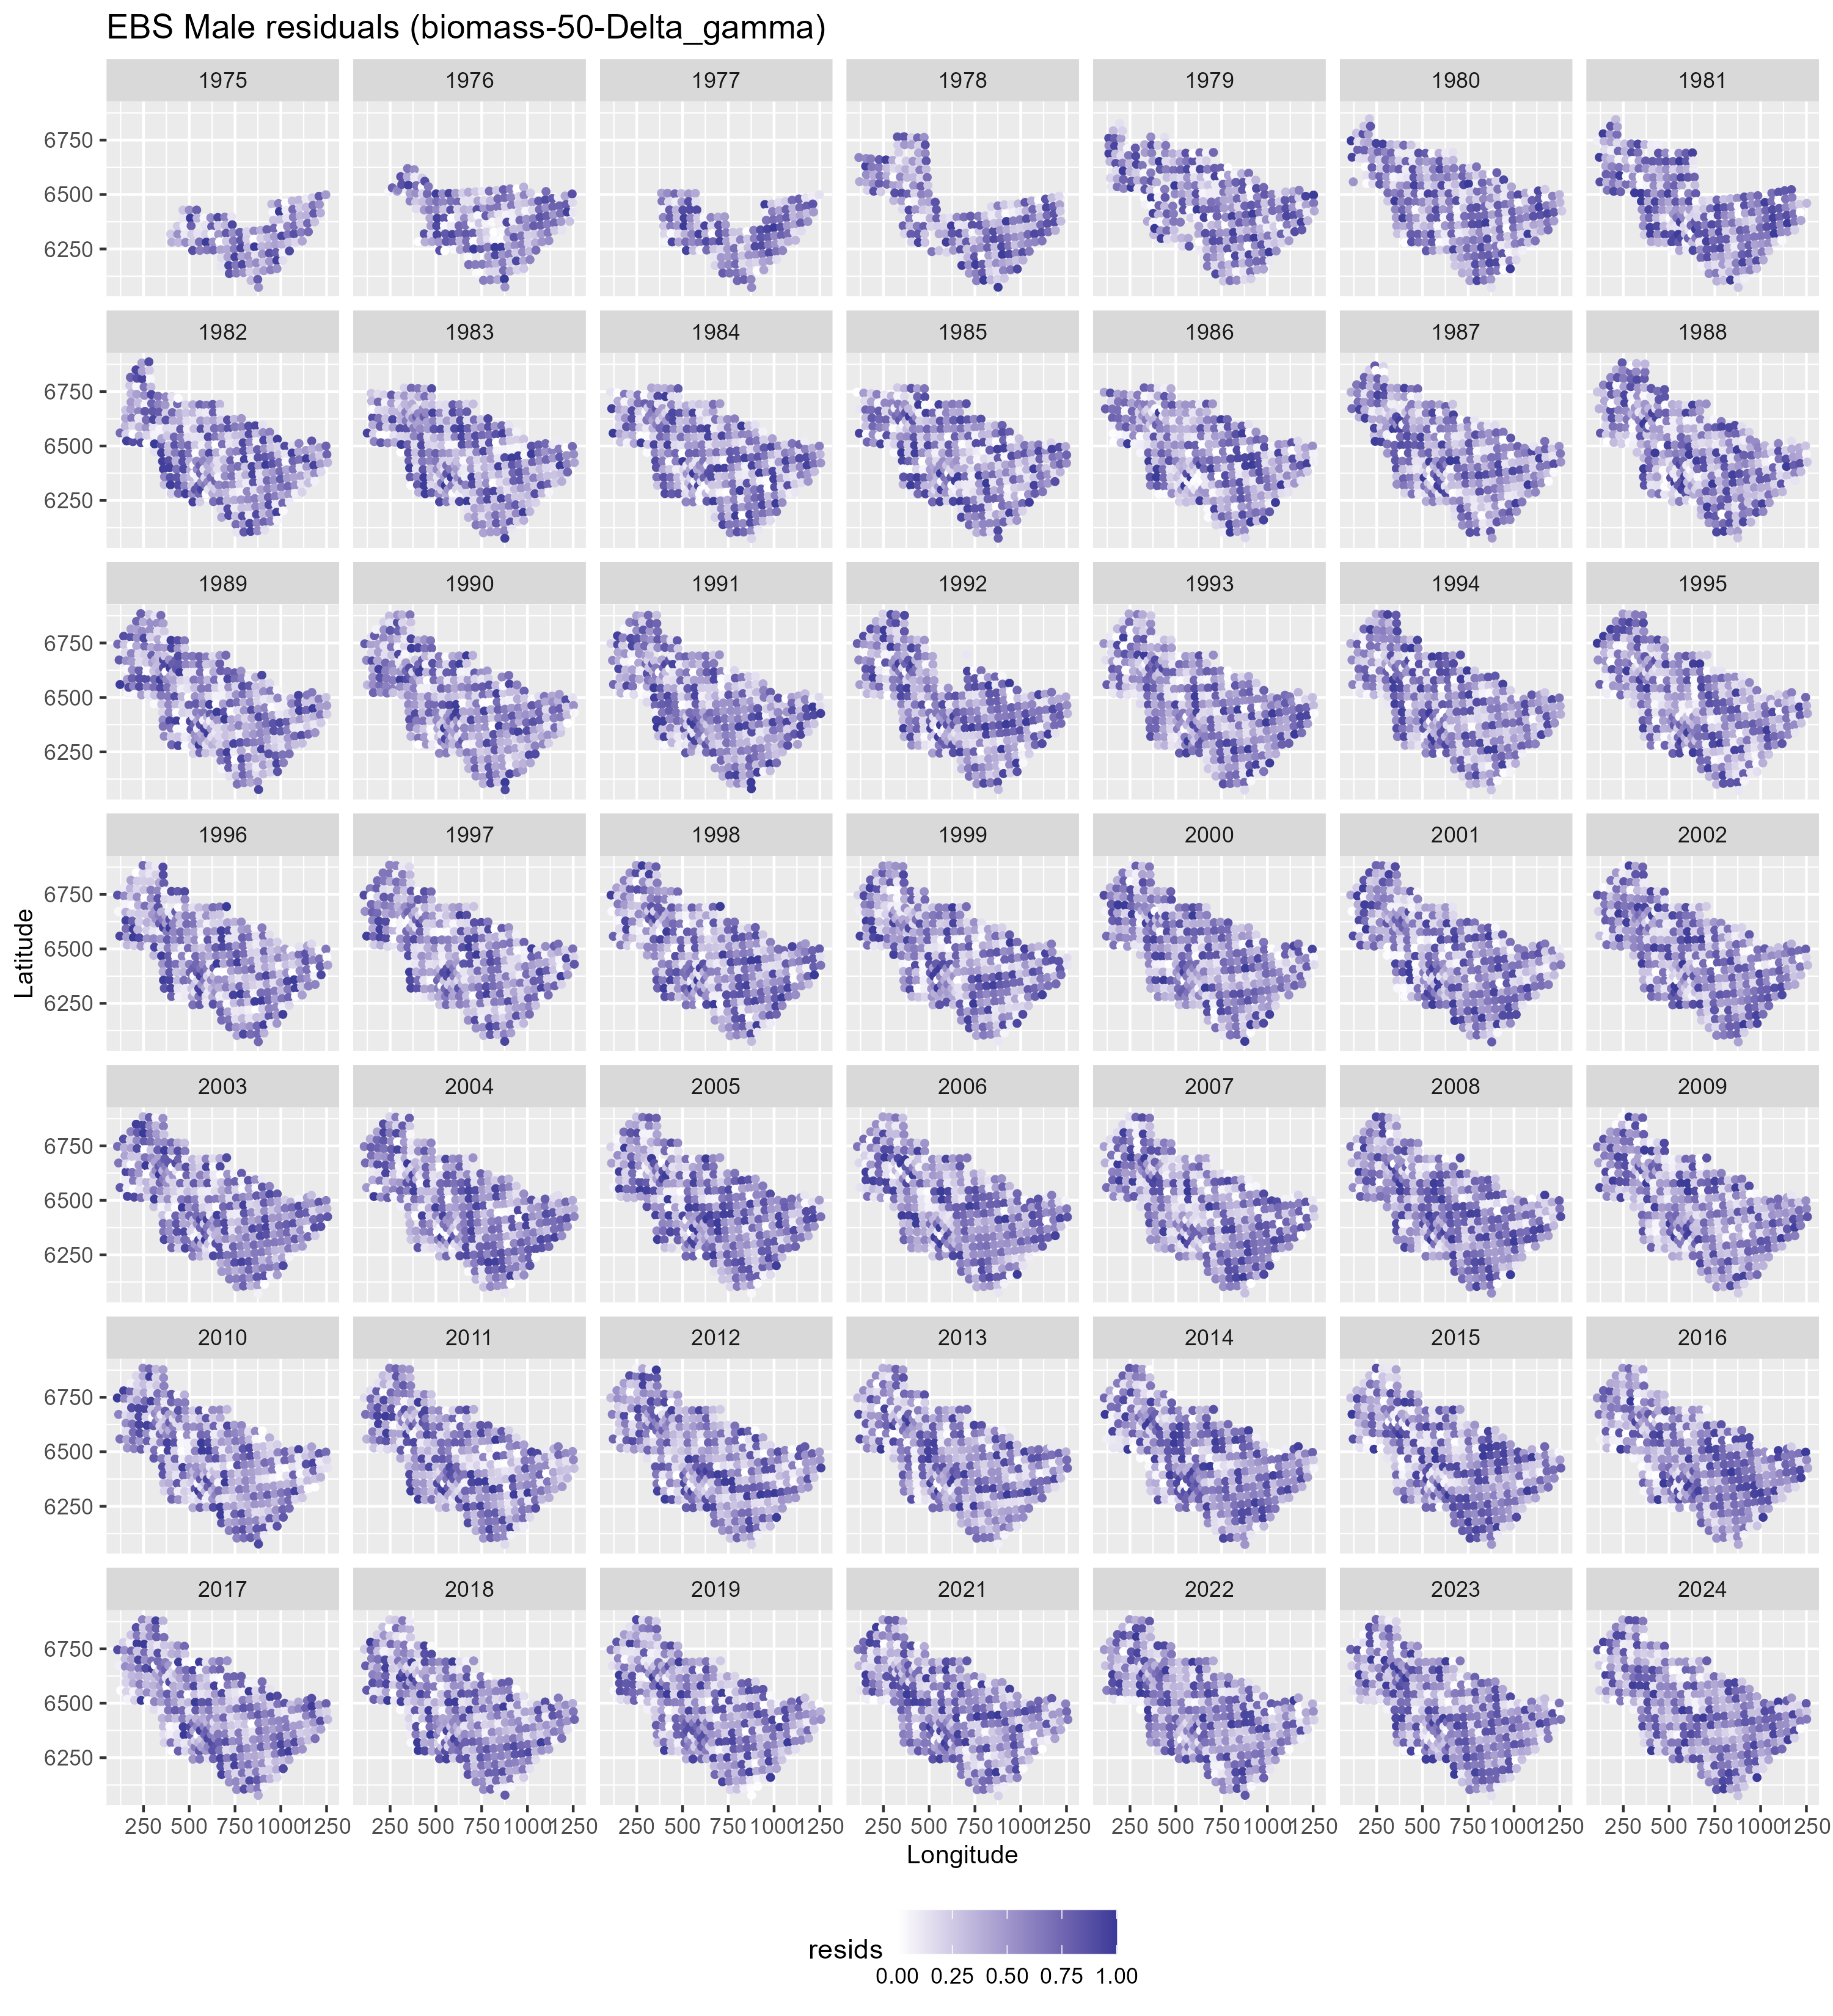
\includegraphics[width=1\linewidth,height=1\textheight]{../BAIRDI/Figures/DHARMa_Male_biomass-50-Delta_gamma_SPATIAL} 

}

\caption{Spatial plot of DHARMa residuals for male biomass models fit using NMFS summer bottom trawl survey data before 1982 and 1982 onward with a 50-knot mesh and a delta-gamma model family. Predictions from both of these periods/models are combined in this figure.}\label{fig:DHARMa-bio-spat-50-male}
\end{figure}

\begin{figure}

{\centering 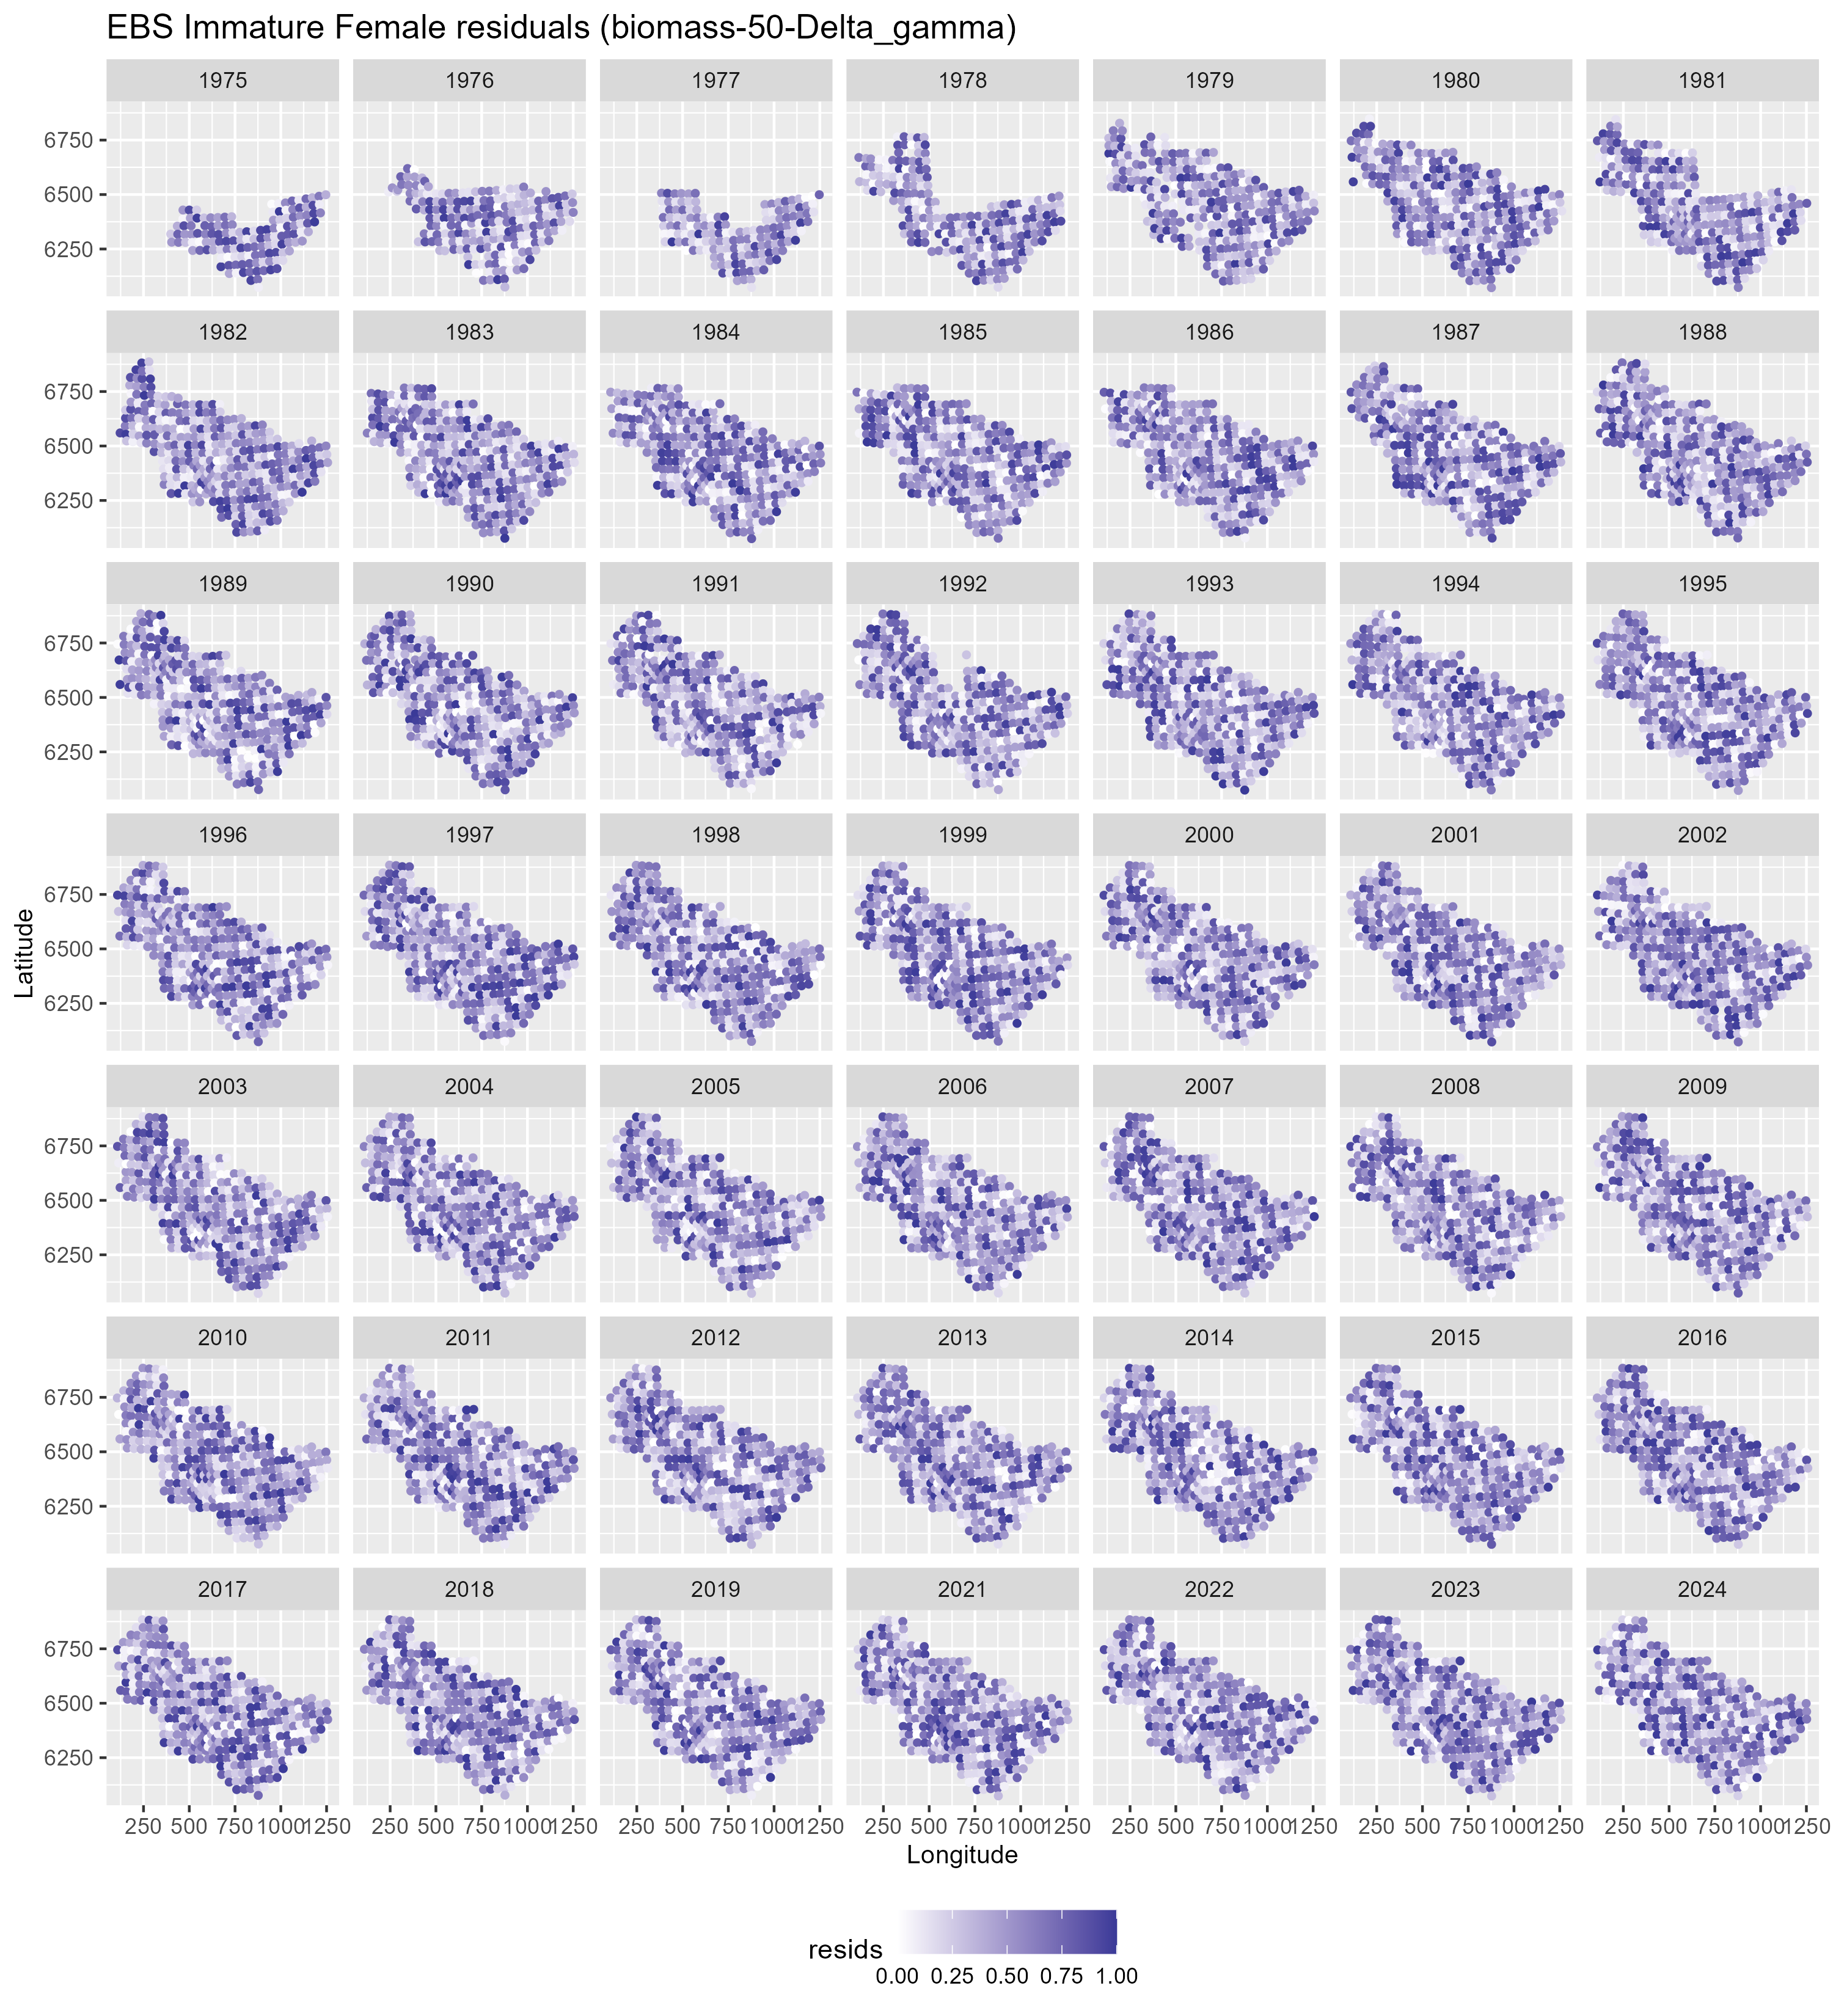
\includegraphics[width=1\linewidth,height=1\textheight]{../BAIRDI/Figures/DHARMa_Immature Female_biomass-50-Delta_gamma_SPATIAL} 

}

\caption{Spatial plot of DHARMa residuals for immature female biomass models fit using NMFS summer bottom trawl survey data before 1982 and 1982 onward with a 50-knot mesh and a delta-gamma model family. Predictions from both of these periods/models are combined in this figure.}\label{fig:DHARMa-bio-spat-50-imfem}
\end{figure}

\begin{figure}

{\centering 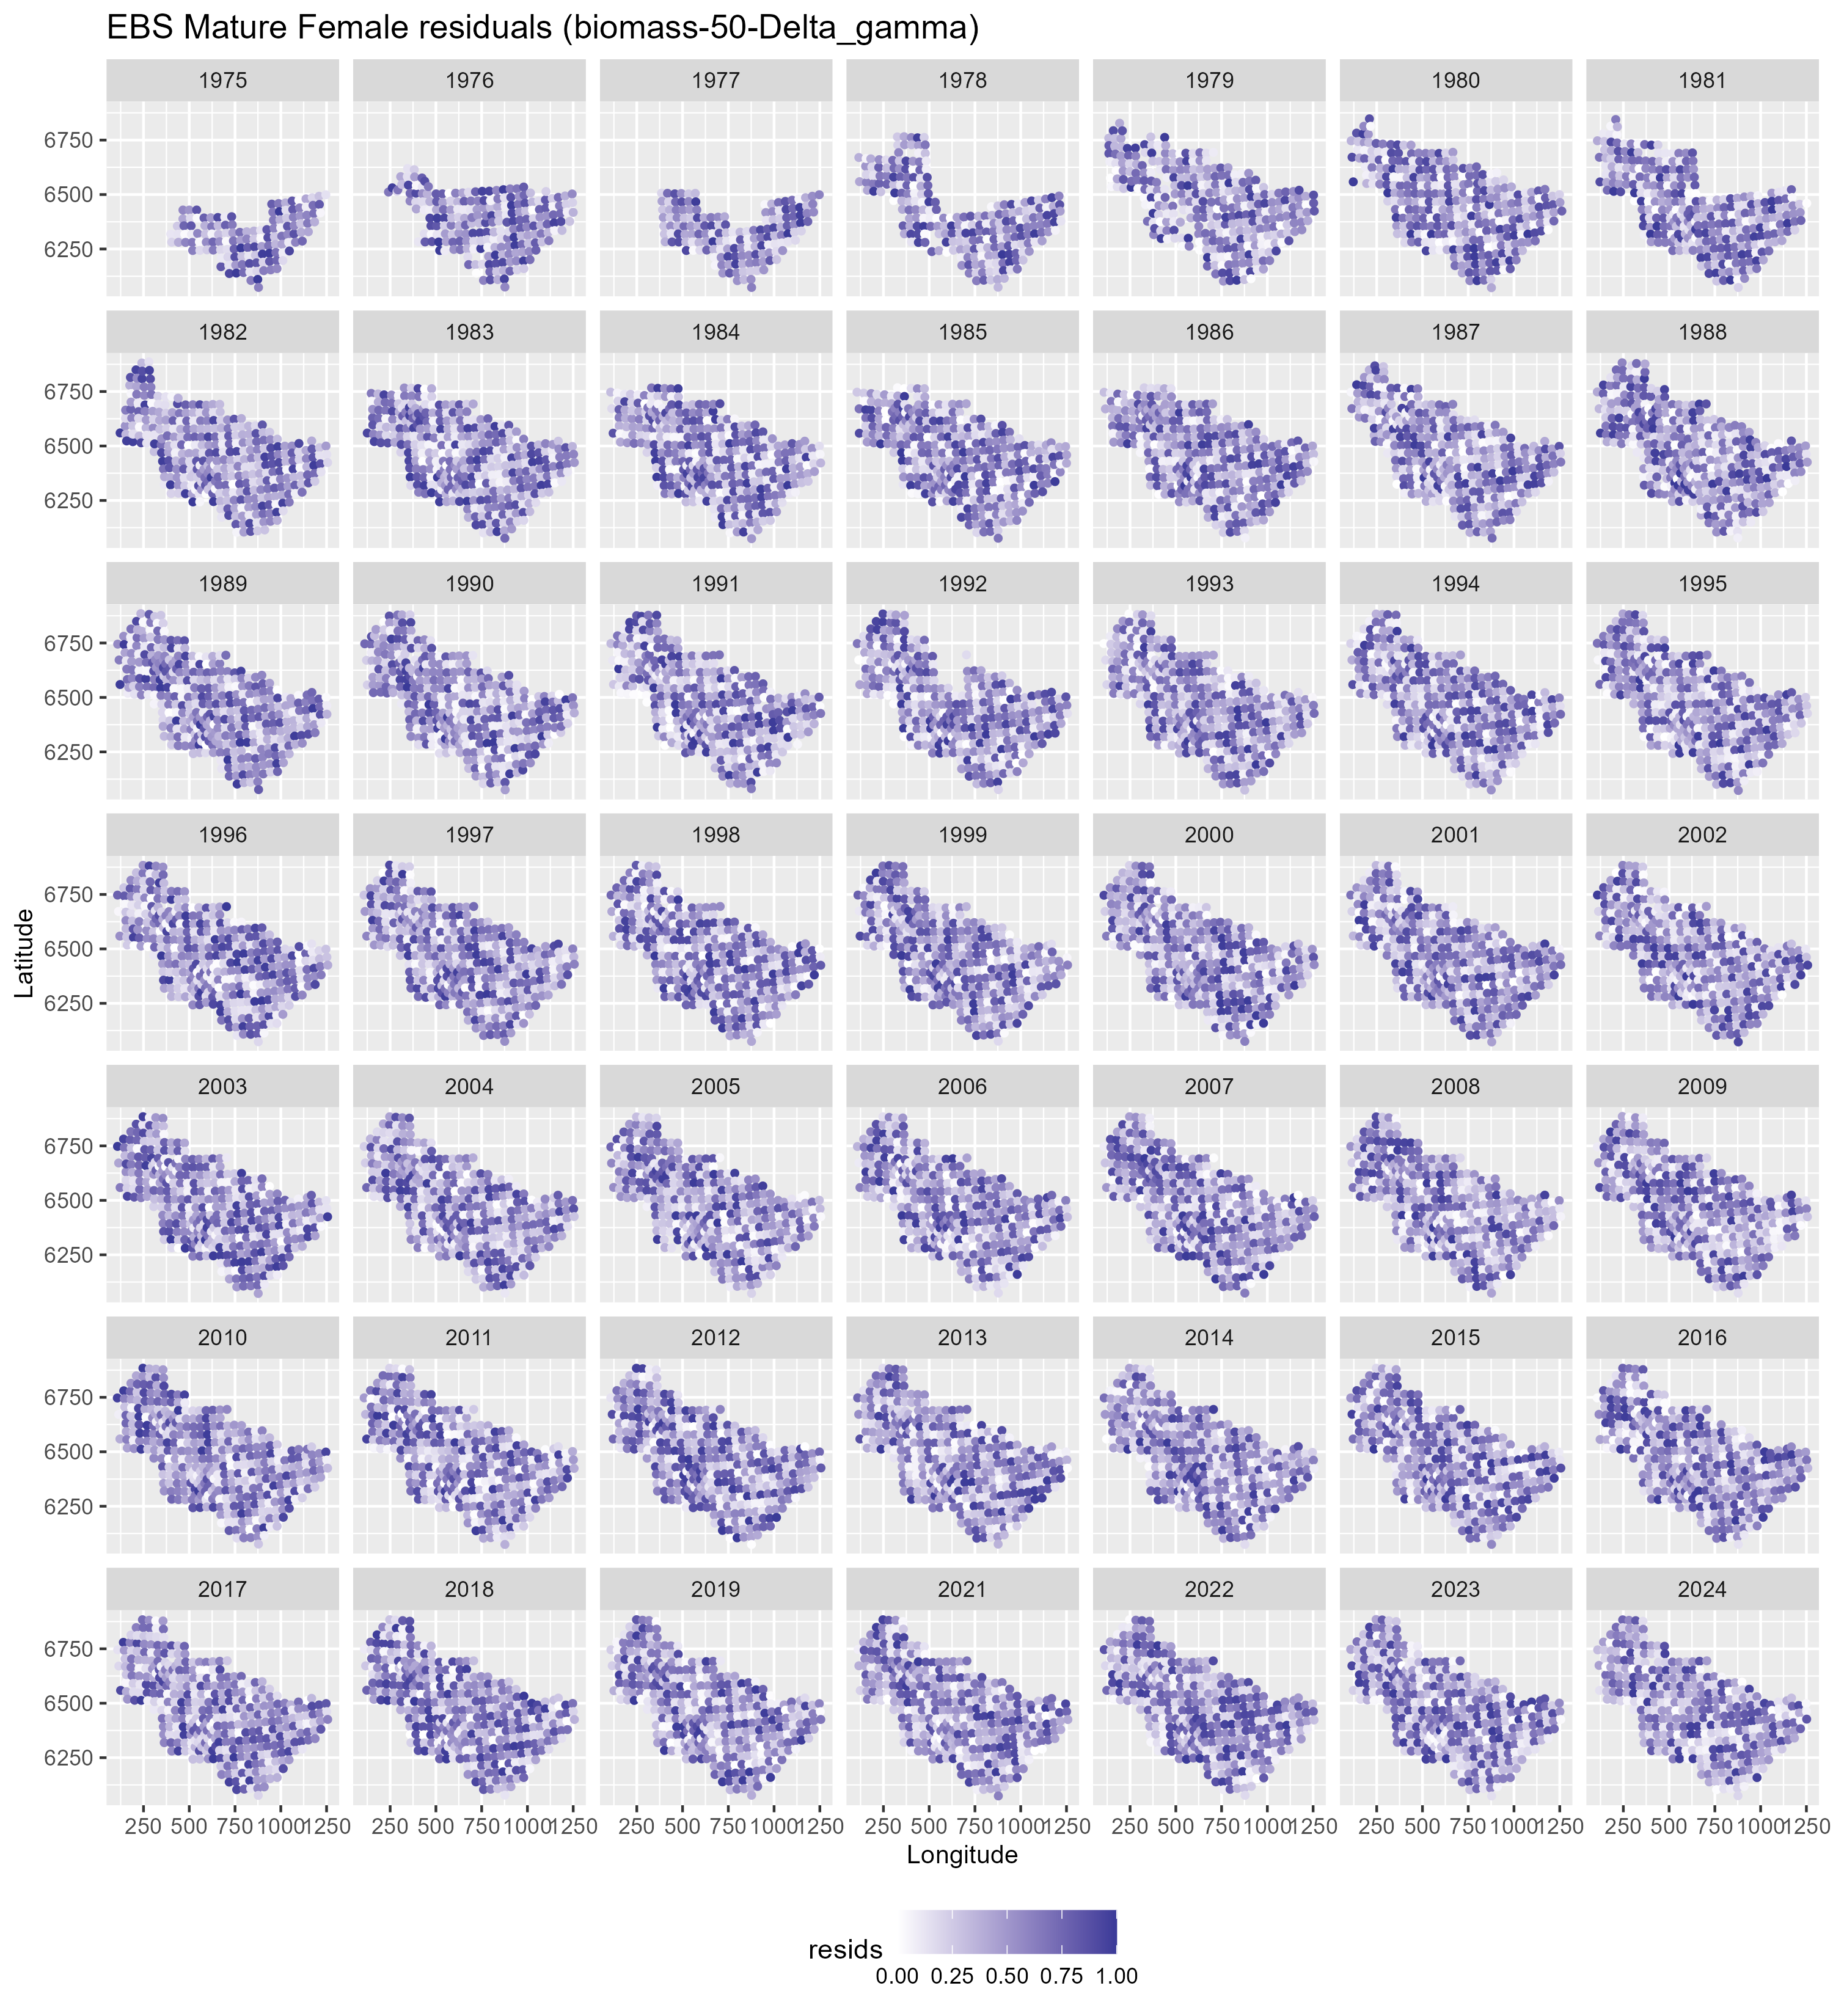
\includegraphics[width=1\linewidth,height=1\textheight]{../BAIRDI/Figures/DHARMa_Mature Female_biomass-50-Delta_gamma_SPATIAL} 

}

\caption{Spatial plot of DHARMa residuals for mature female biomass models fit using NMFS summer bottom trawl survey data before 1982 and 1982 onward with a 50-knot mesh and a delta-gamma model family. Predictions from both of these periods/models are combined in this figure.}\label{fig:DHARMa-bio-spat-50-matfem}
\end{figure}

\begin{figure}

{\centering 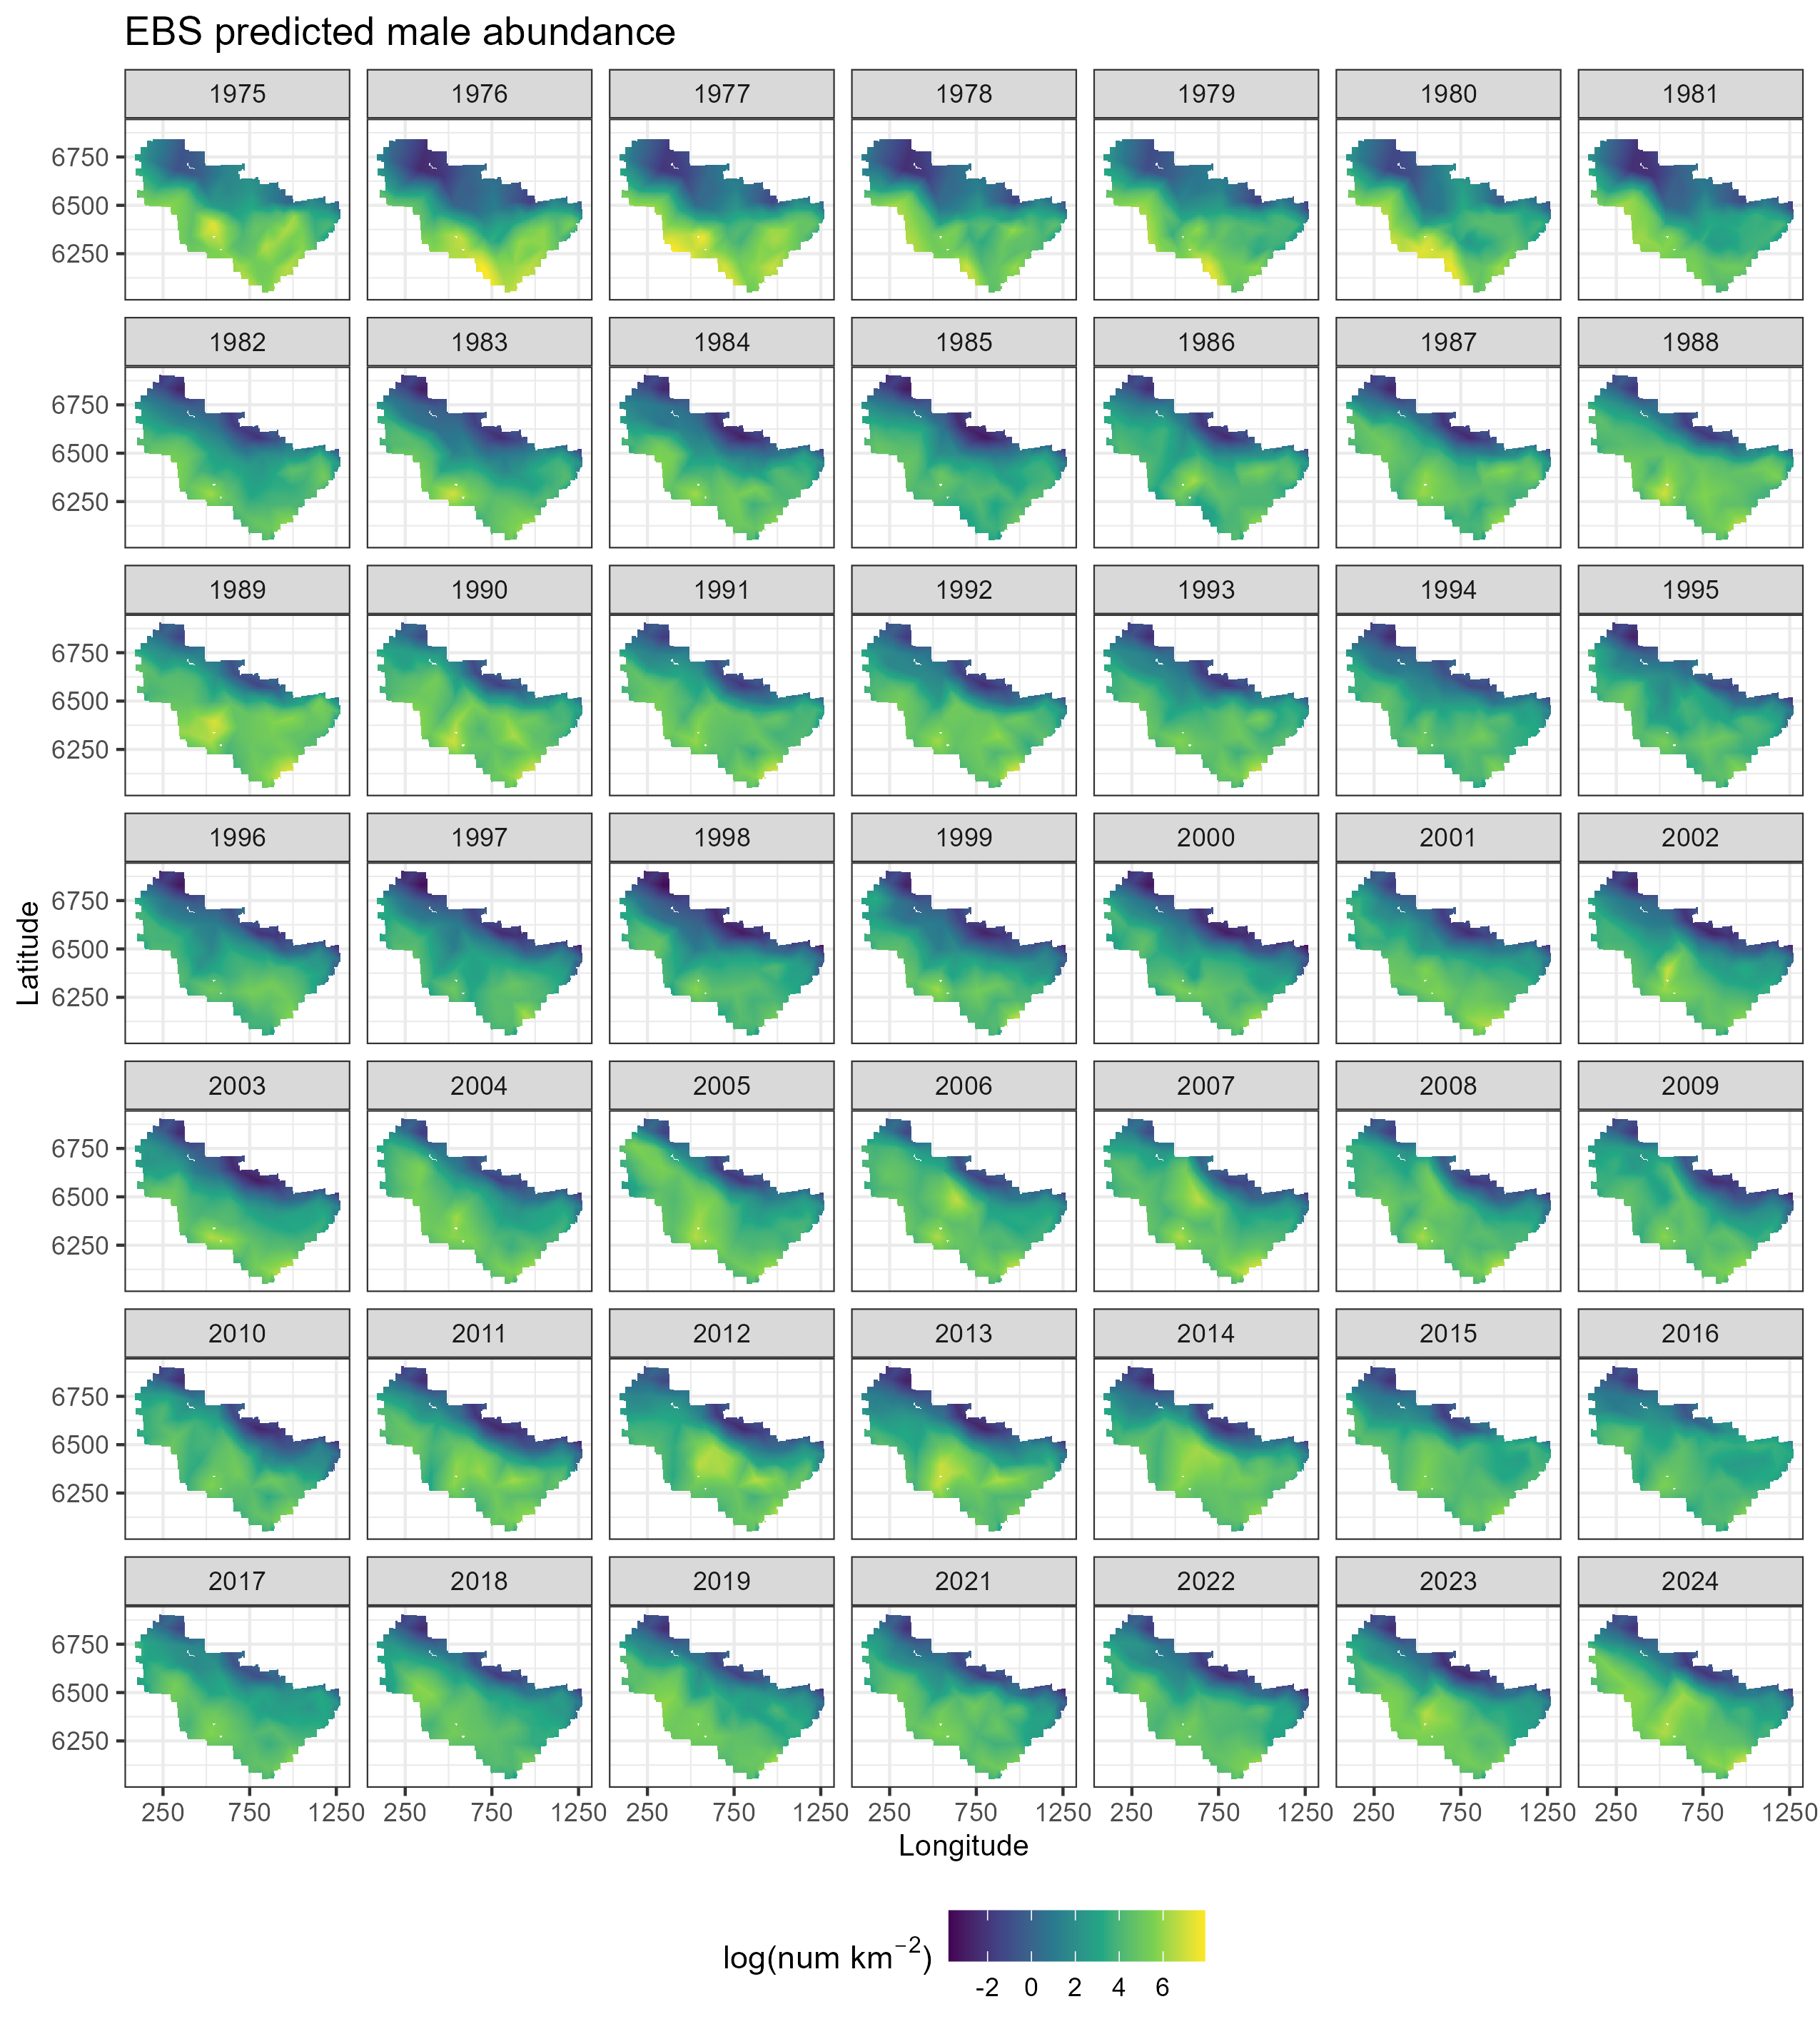
\includegraphics[width=1\linewidth,height=1\textheight]{../BAIRDI/Figures/EBS_male_spatabund} 

}

\caption{Spatial predictions of male abundance across the eastern Bering Sea using NMFS summer bottom trawl survey data before 1982 and 1982 onward with a 50-knot mesh and a delta-gamma model family. Predictions from both of these periods/models are combined in this figure.}\label{fig:spatpred-abund-50-male}
\end{figure}

\begin{figure}

{\centering 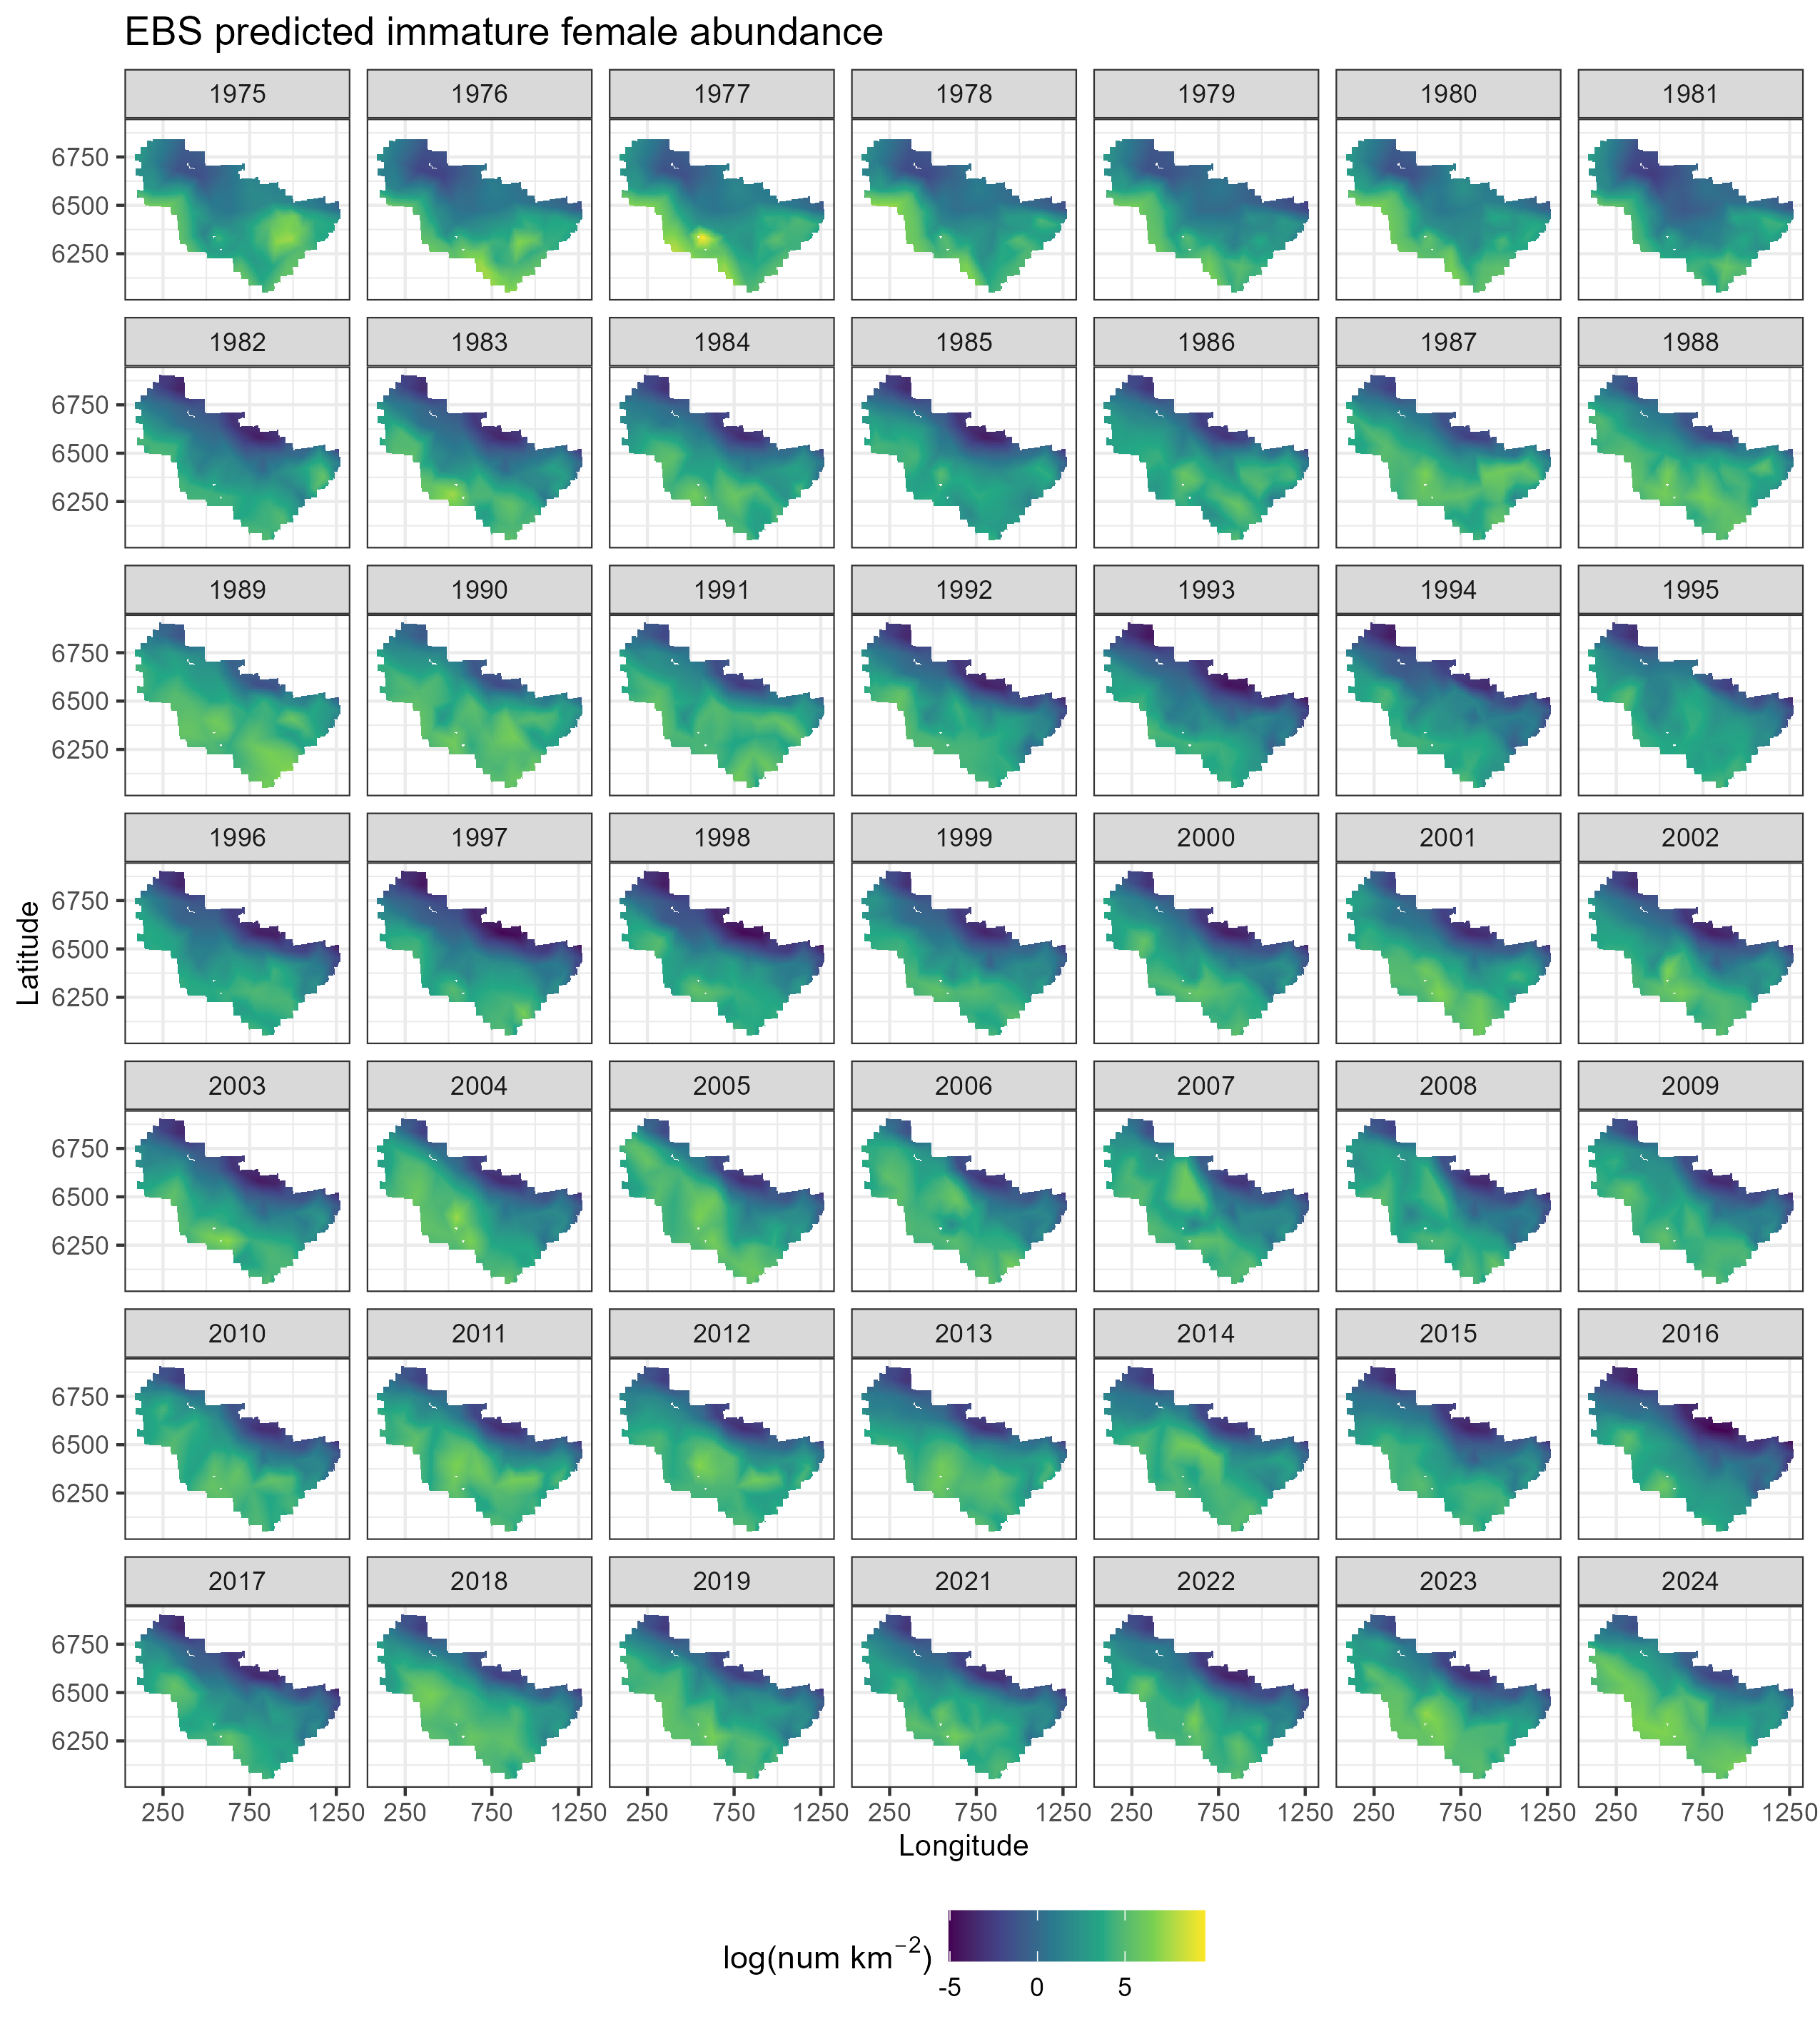
\includegraphics[width=1\linewidth,height=1\textheight]{../BAIRDI/Figures/EBS_imfem_spatabund} 

}

\caption{Spatial predictions of immature female abundance across the eastern Bering Sea using NMFS summer bottom trawl survey data before 1982 and 1982 onward with a 50-knot mesh and a delta-gamma model family. Predictions from both of these periods/models are combined in this figure.}\label{fig:spatpred-abund-50-imfem}
\end{figure}

\begin{figure}

{\centering 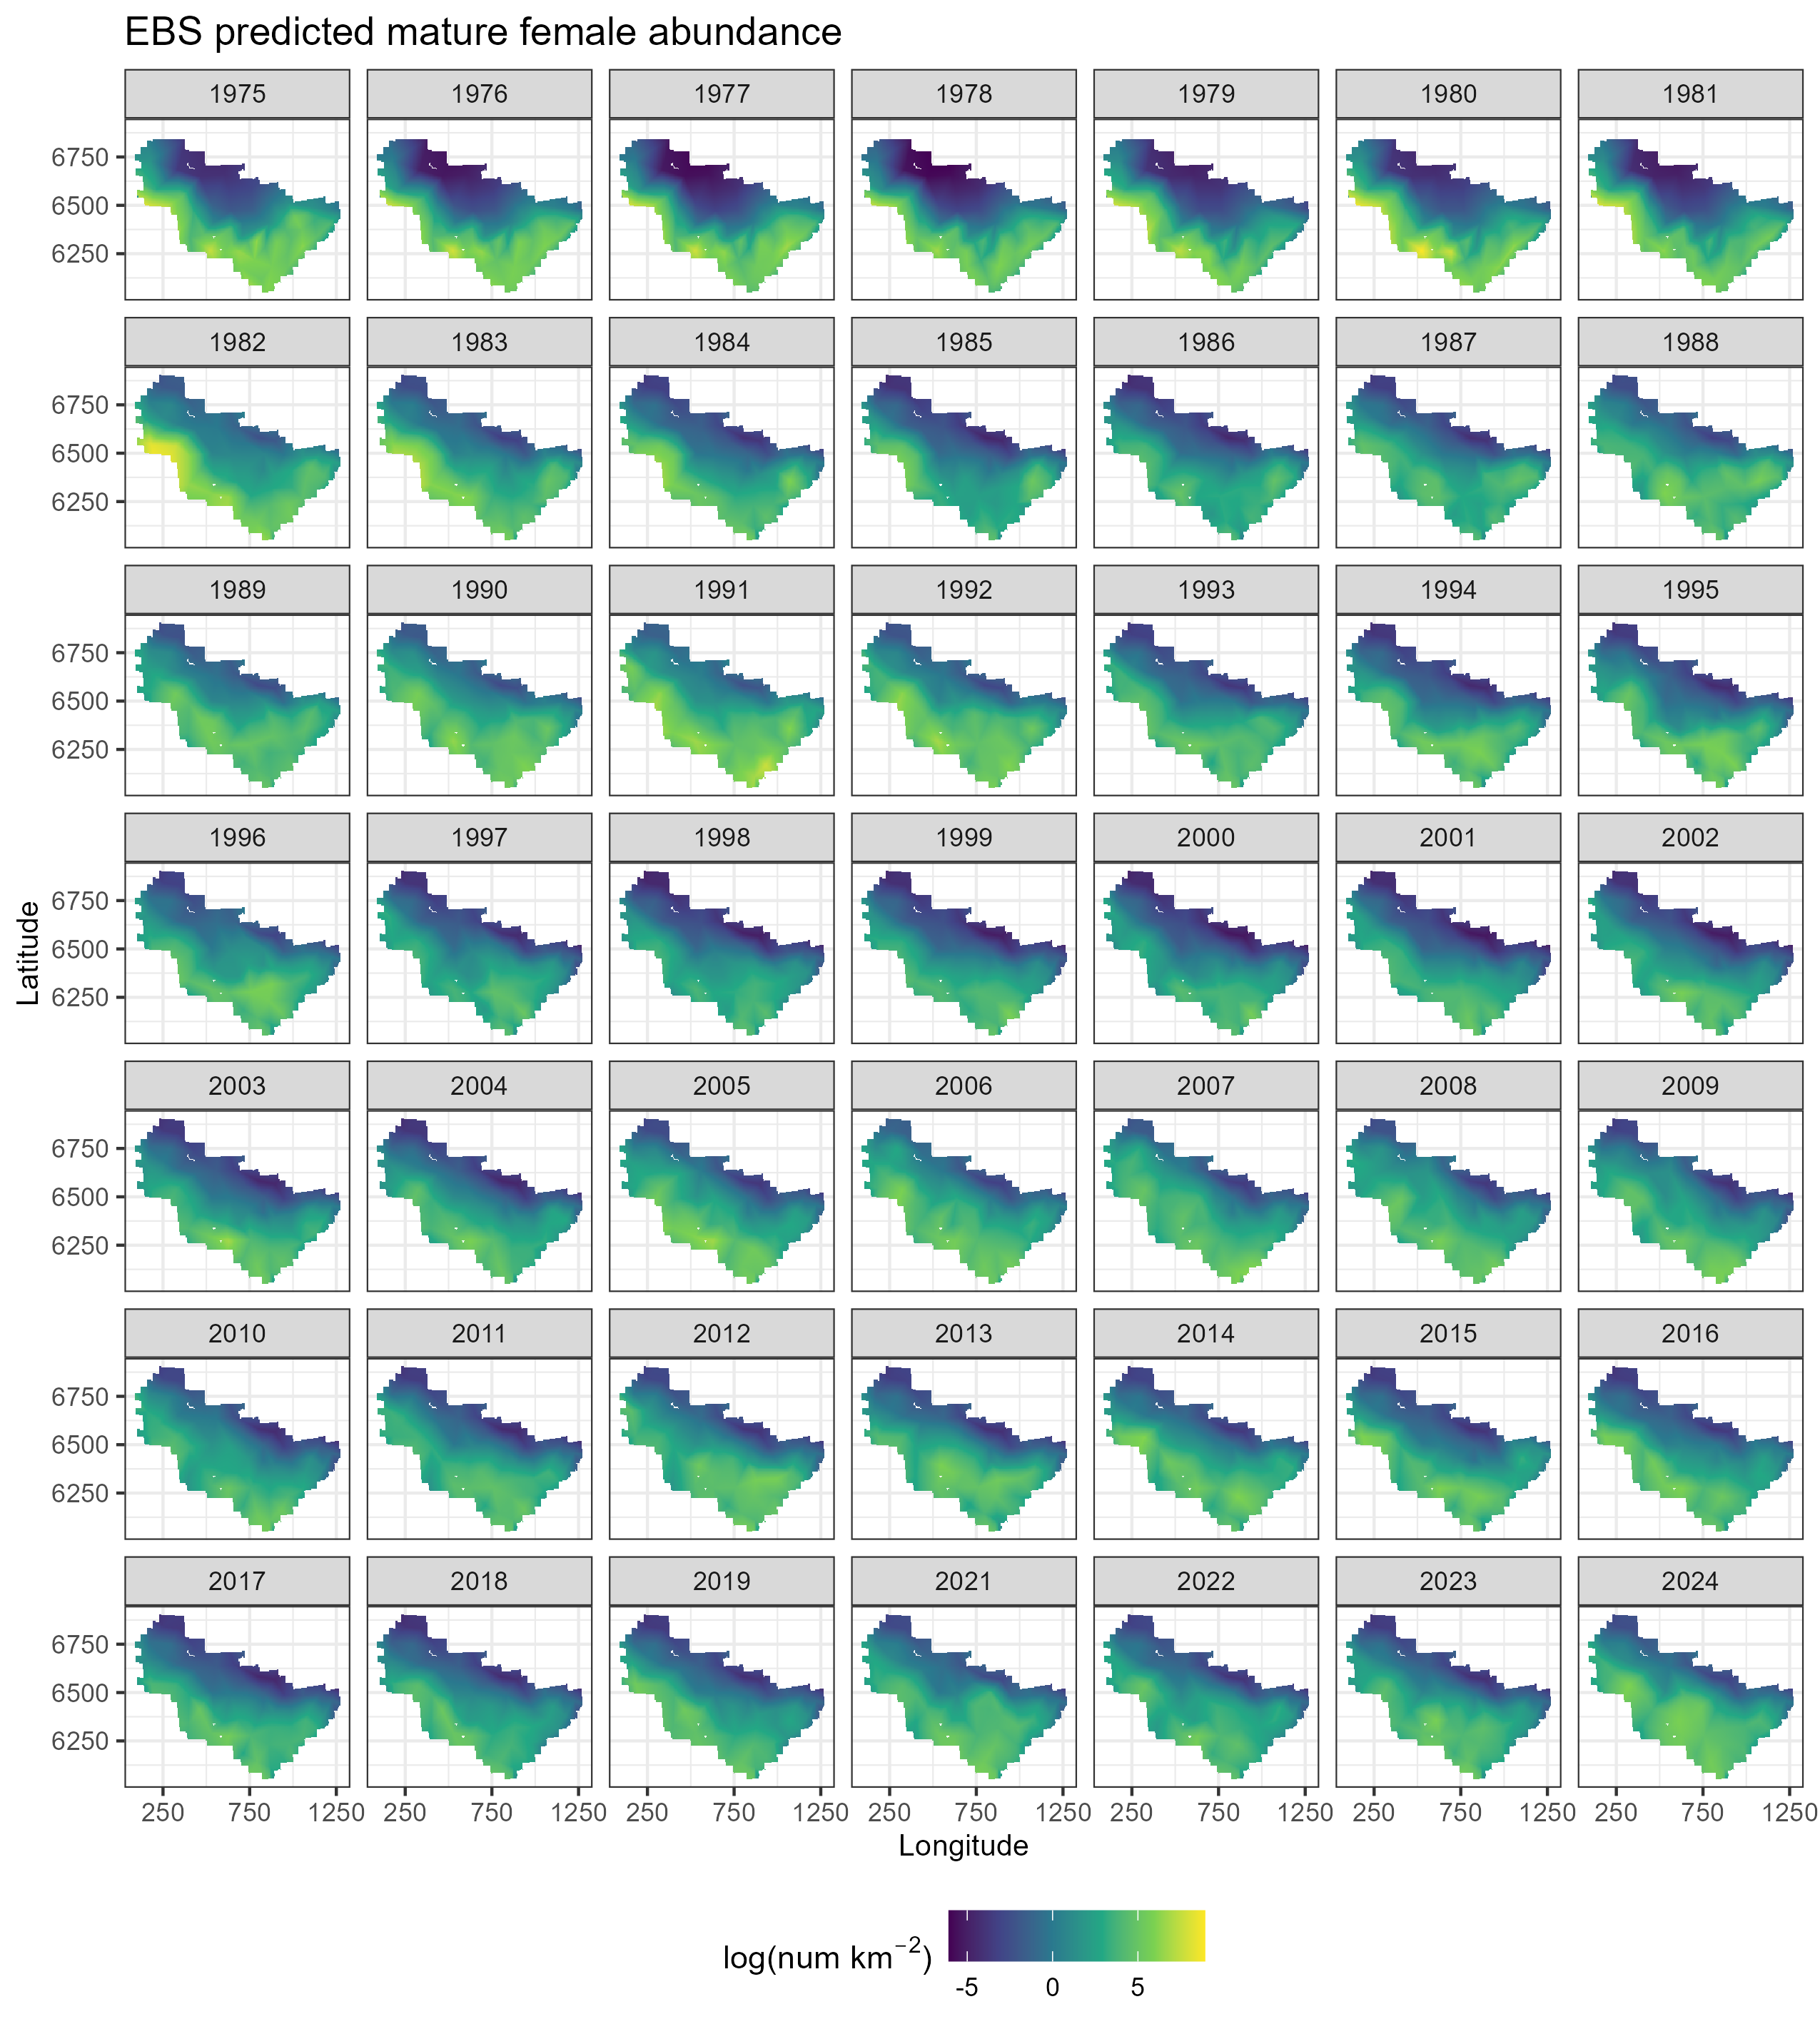
\includegraphics[width=1\linewidth,height=1\textheight]{../BAIRDI/Figures/EBS_matfem_spatabund} 

}

\caption{Spatial predictions of mature female abundance across the eastern Bering Sea using NMFS summer bottom trawl survey data before 1982 and 1982 onward with a 50-knot mesh and a delta-gamma model family. Predictions from both of these periods/models are combined in this figure.}\label{fig:spatpred-abund-50-matfem}
\end{figure}

\begin{figure}

{\centering 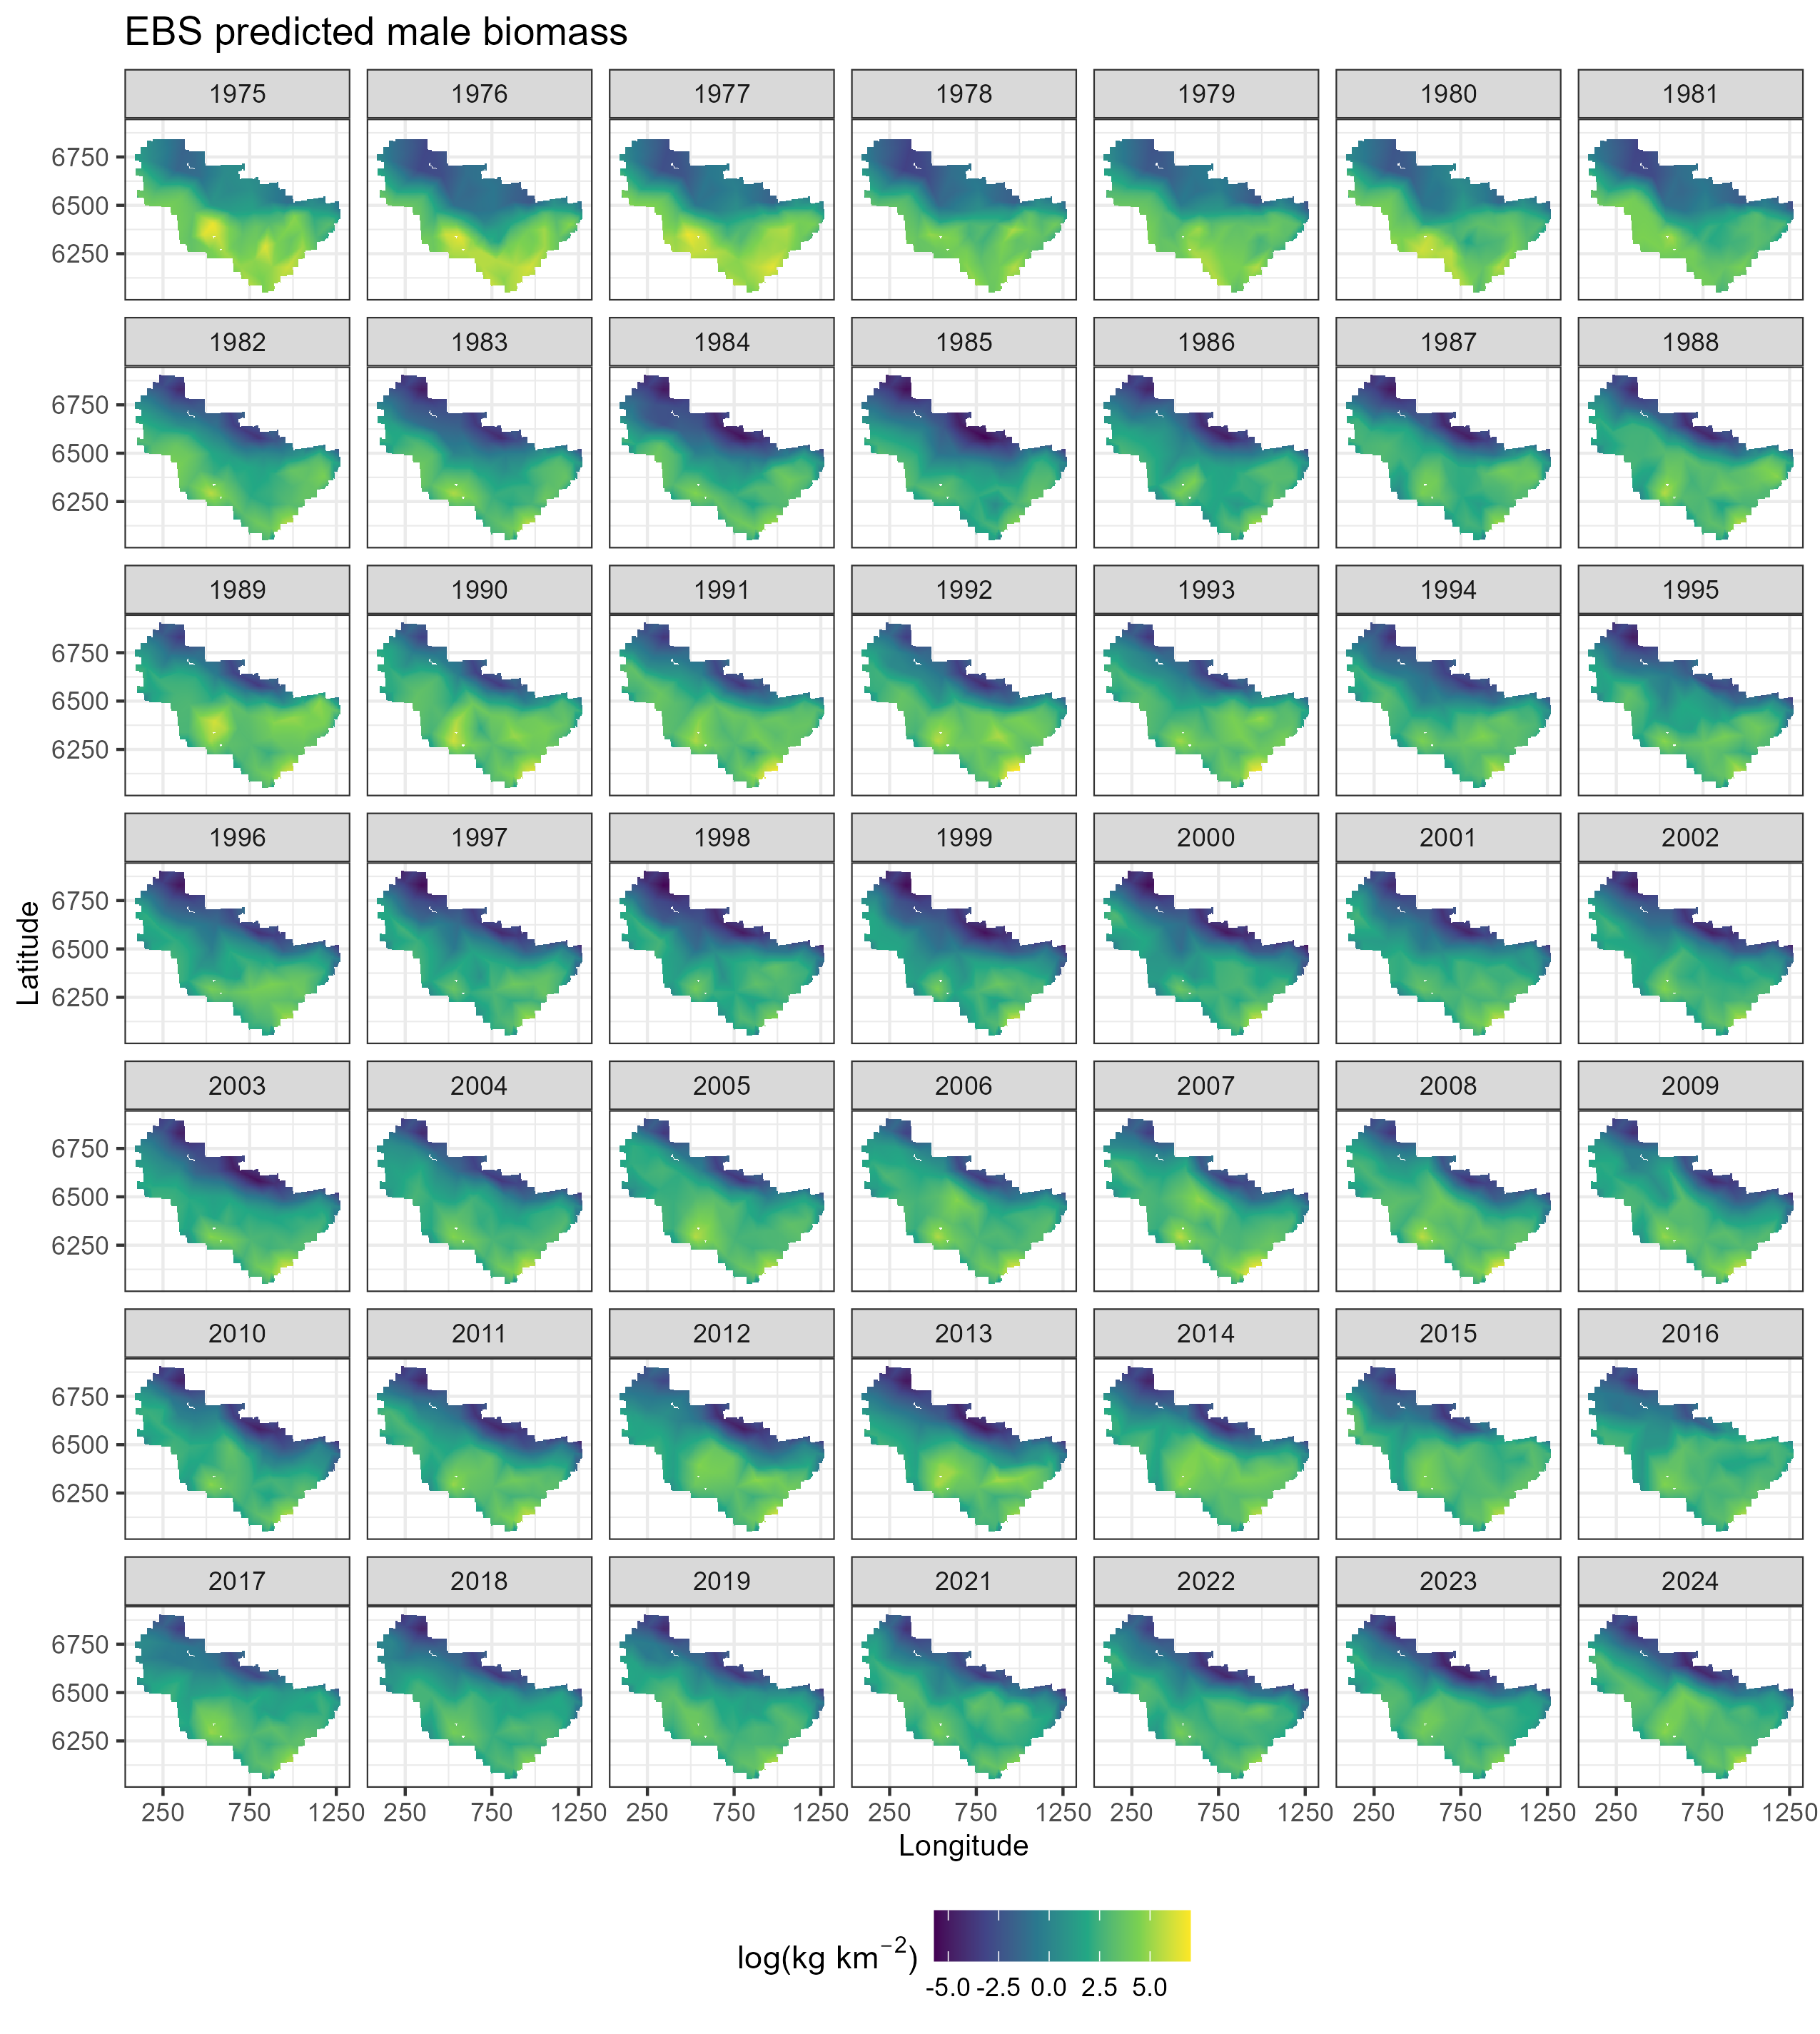
\includegraphics[width=1\linewidth,height=1\textheight]{../BAIRDI/Figures/EBS_male_spatbio} 

}

\caption{Spatial predictions of male biomass across the eastern Bering Sea using NMFS summer bottom trawl survey data before 1982 and 1982 onward with a 50-knot mesh and a delta-gamma model family. Predictions from both of these periods/models are combined in this figure.}\label{fig:spatpred-bio-50-male}
\end{figure}

\begin{figure}

{\centering 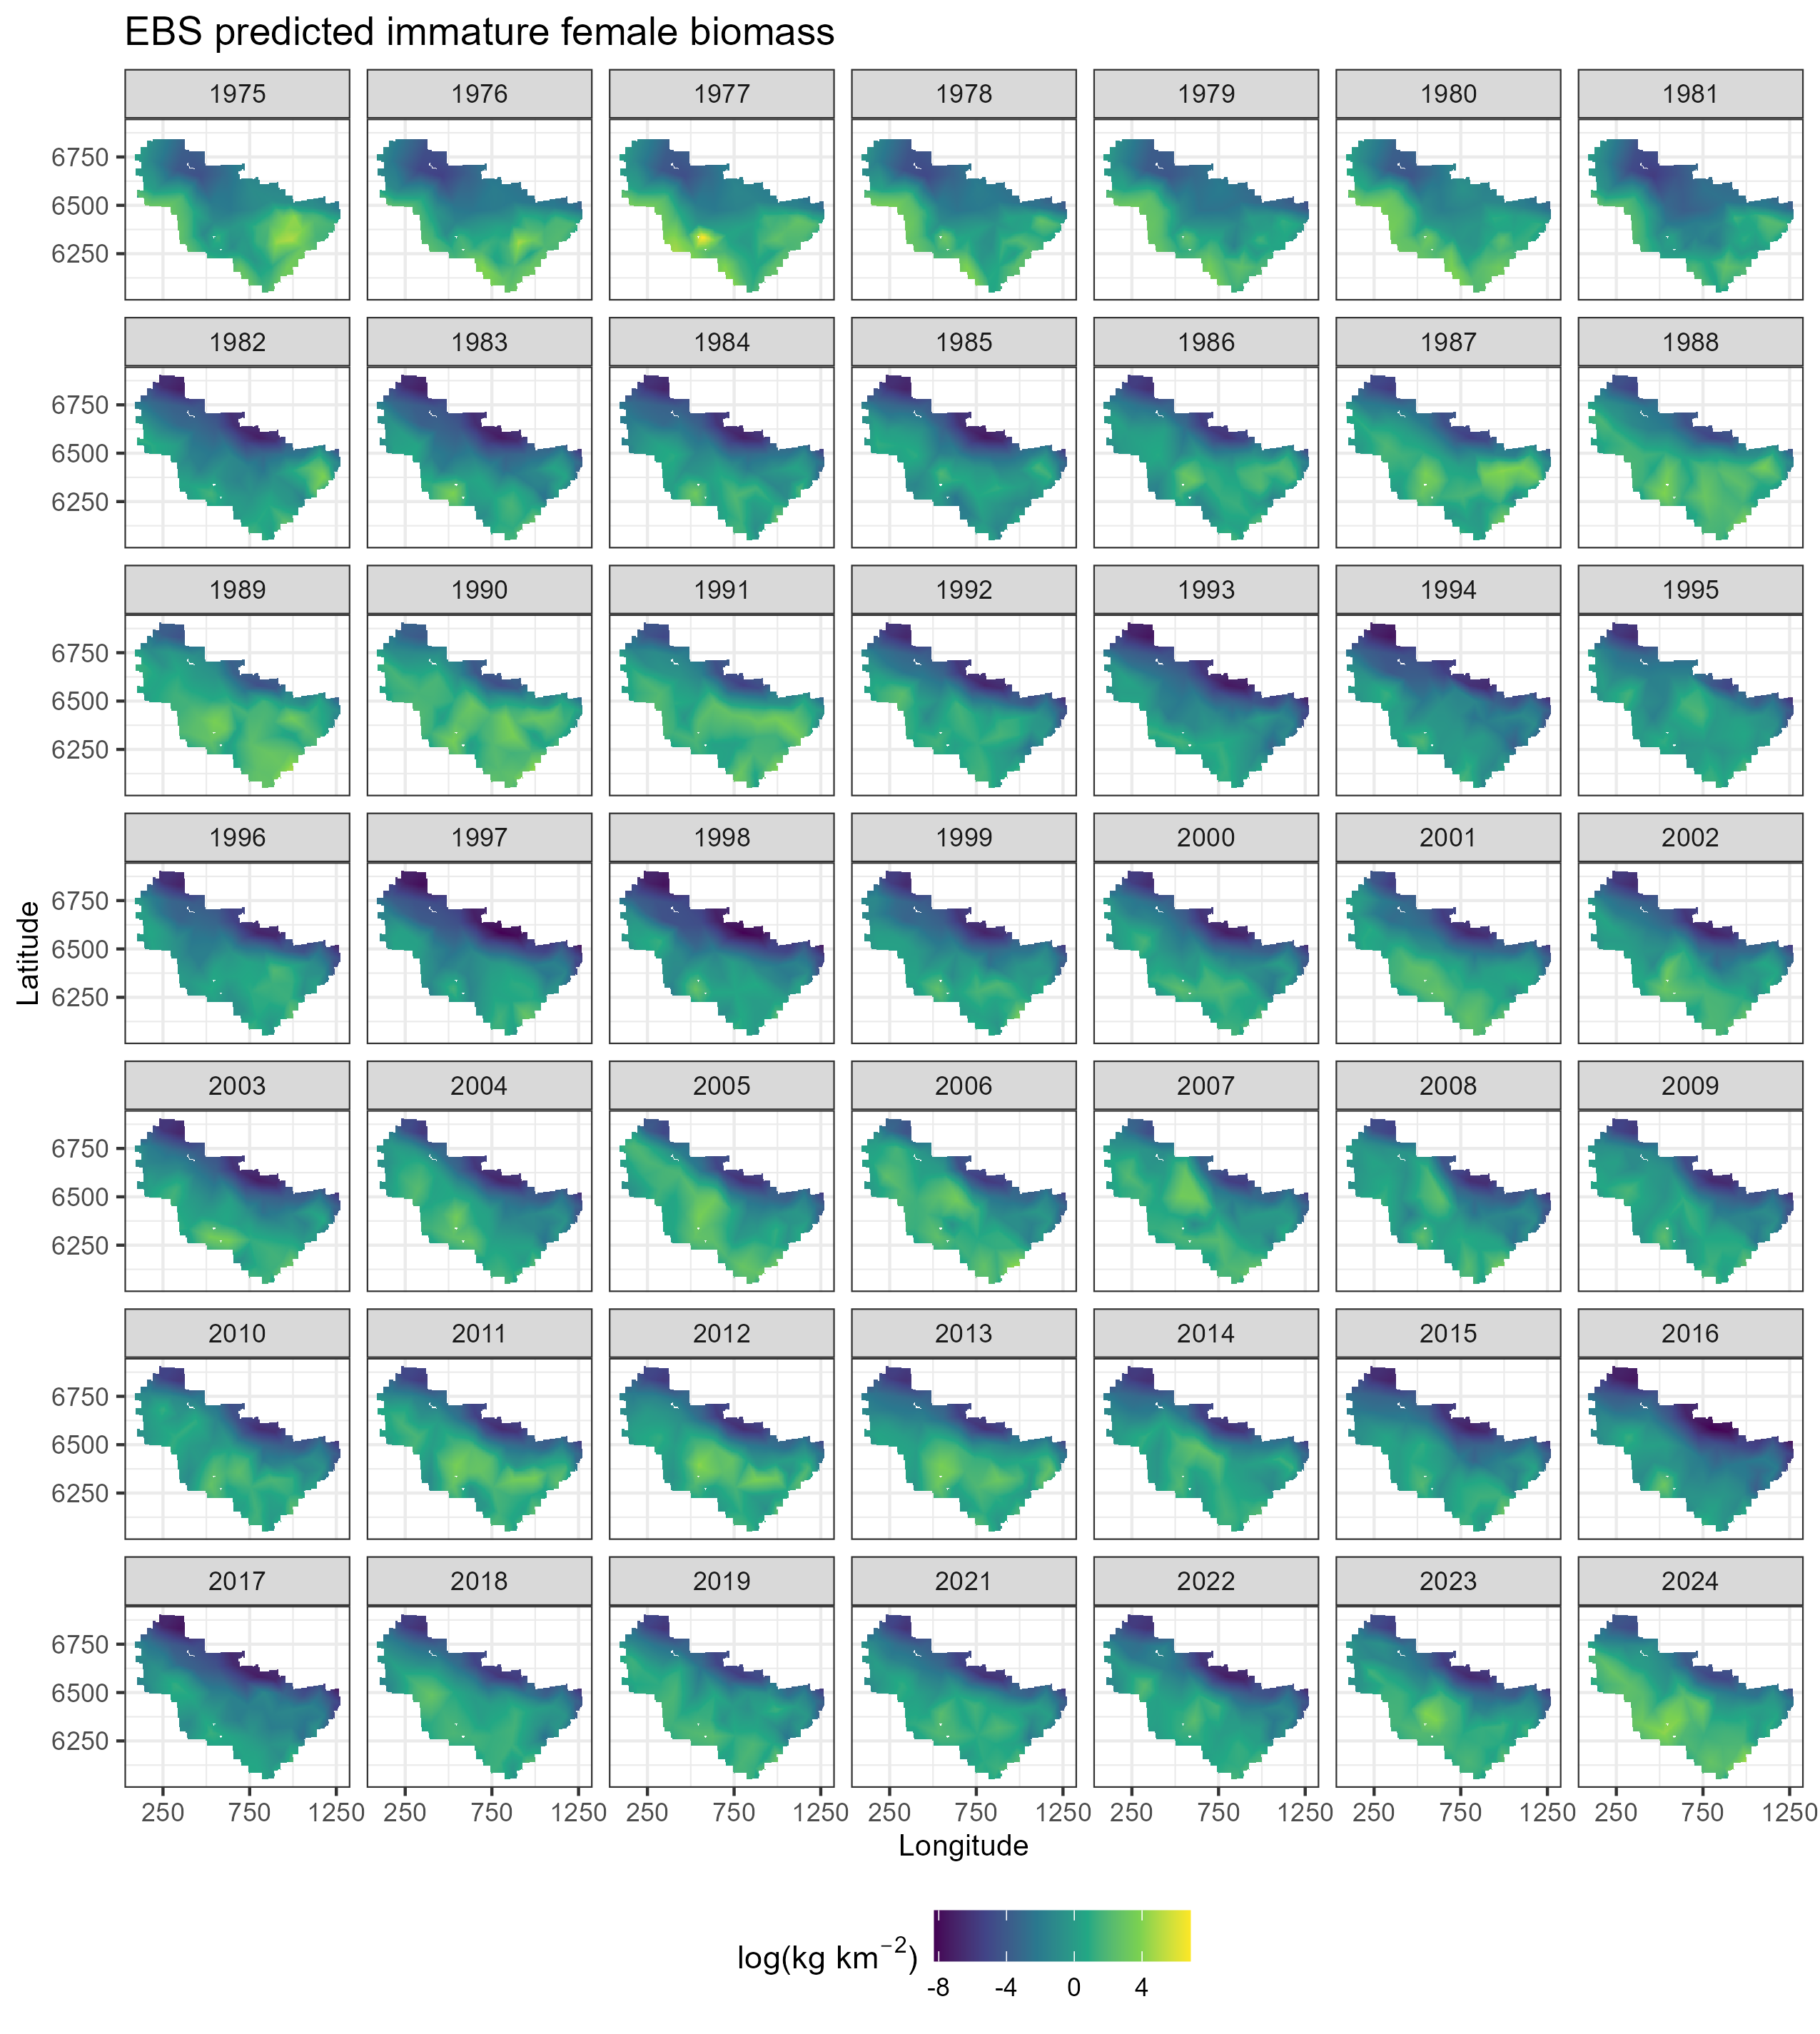
\includegraphics[width=1\linewidth,height=1\textheight]{../BAIRDI/Figures/EBS_imfem_spatbio} 

}

\caption{Spatial predictions of immature female biomass across the eastern Bering Sea using NMFS summer bottom trawl survey data before 1982 and 1982 onward with a 50-knot mesh and a delta-gamma model family. Predictions from both of these periods/models are combined in this figure.}\label{fig:spatpred-bio-50-imfem}
\end{figure}

\begin{figure}

{\centering 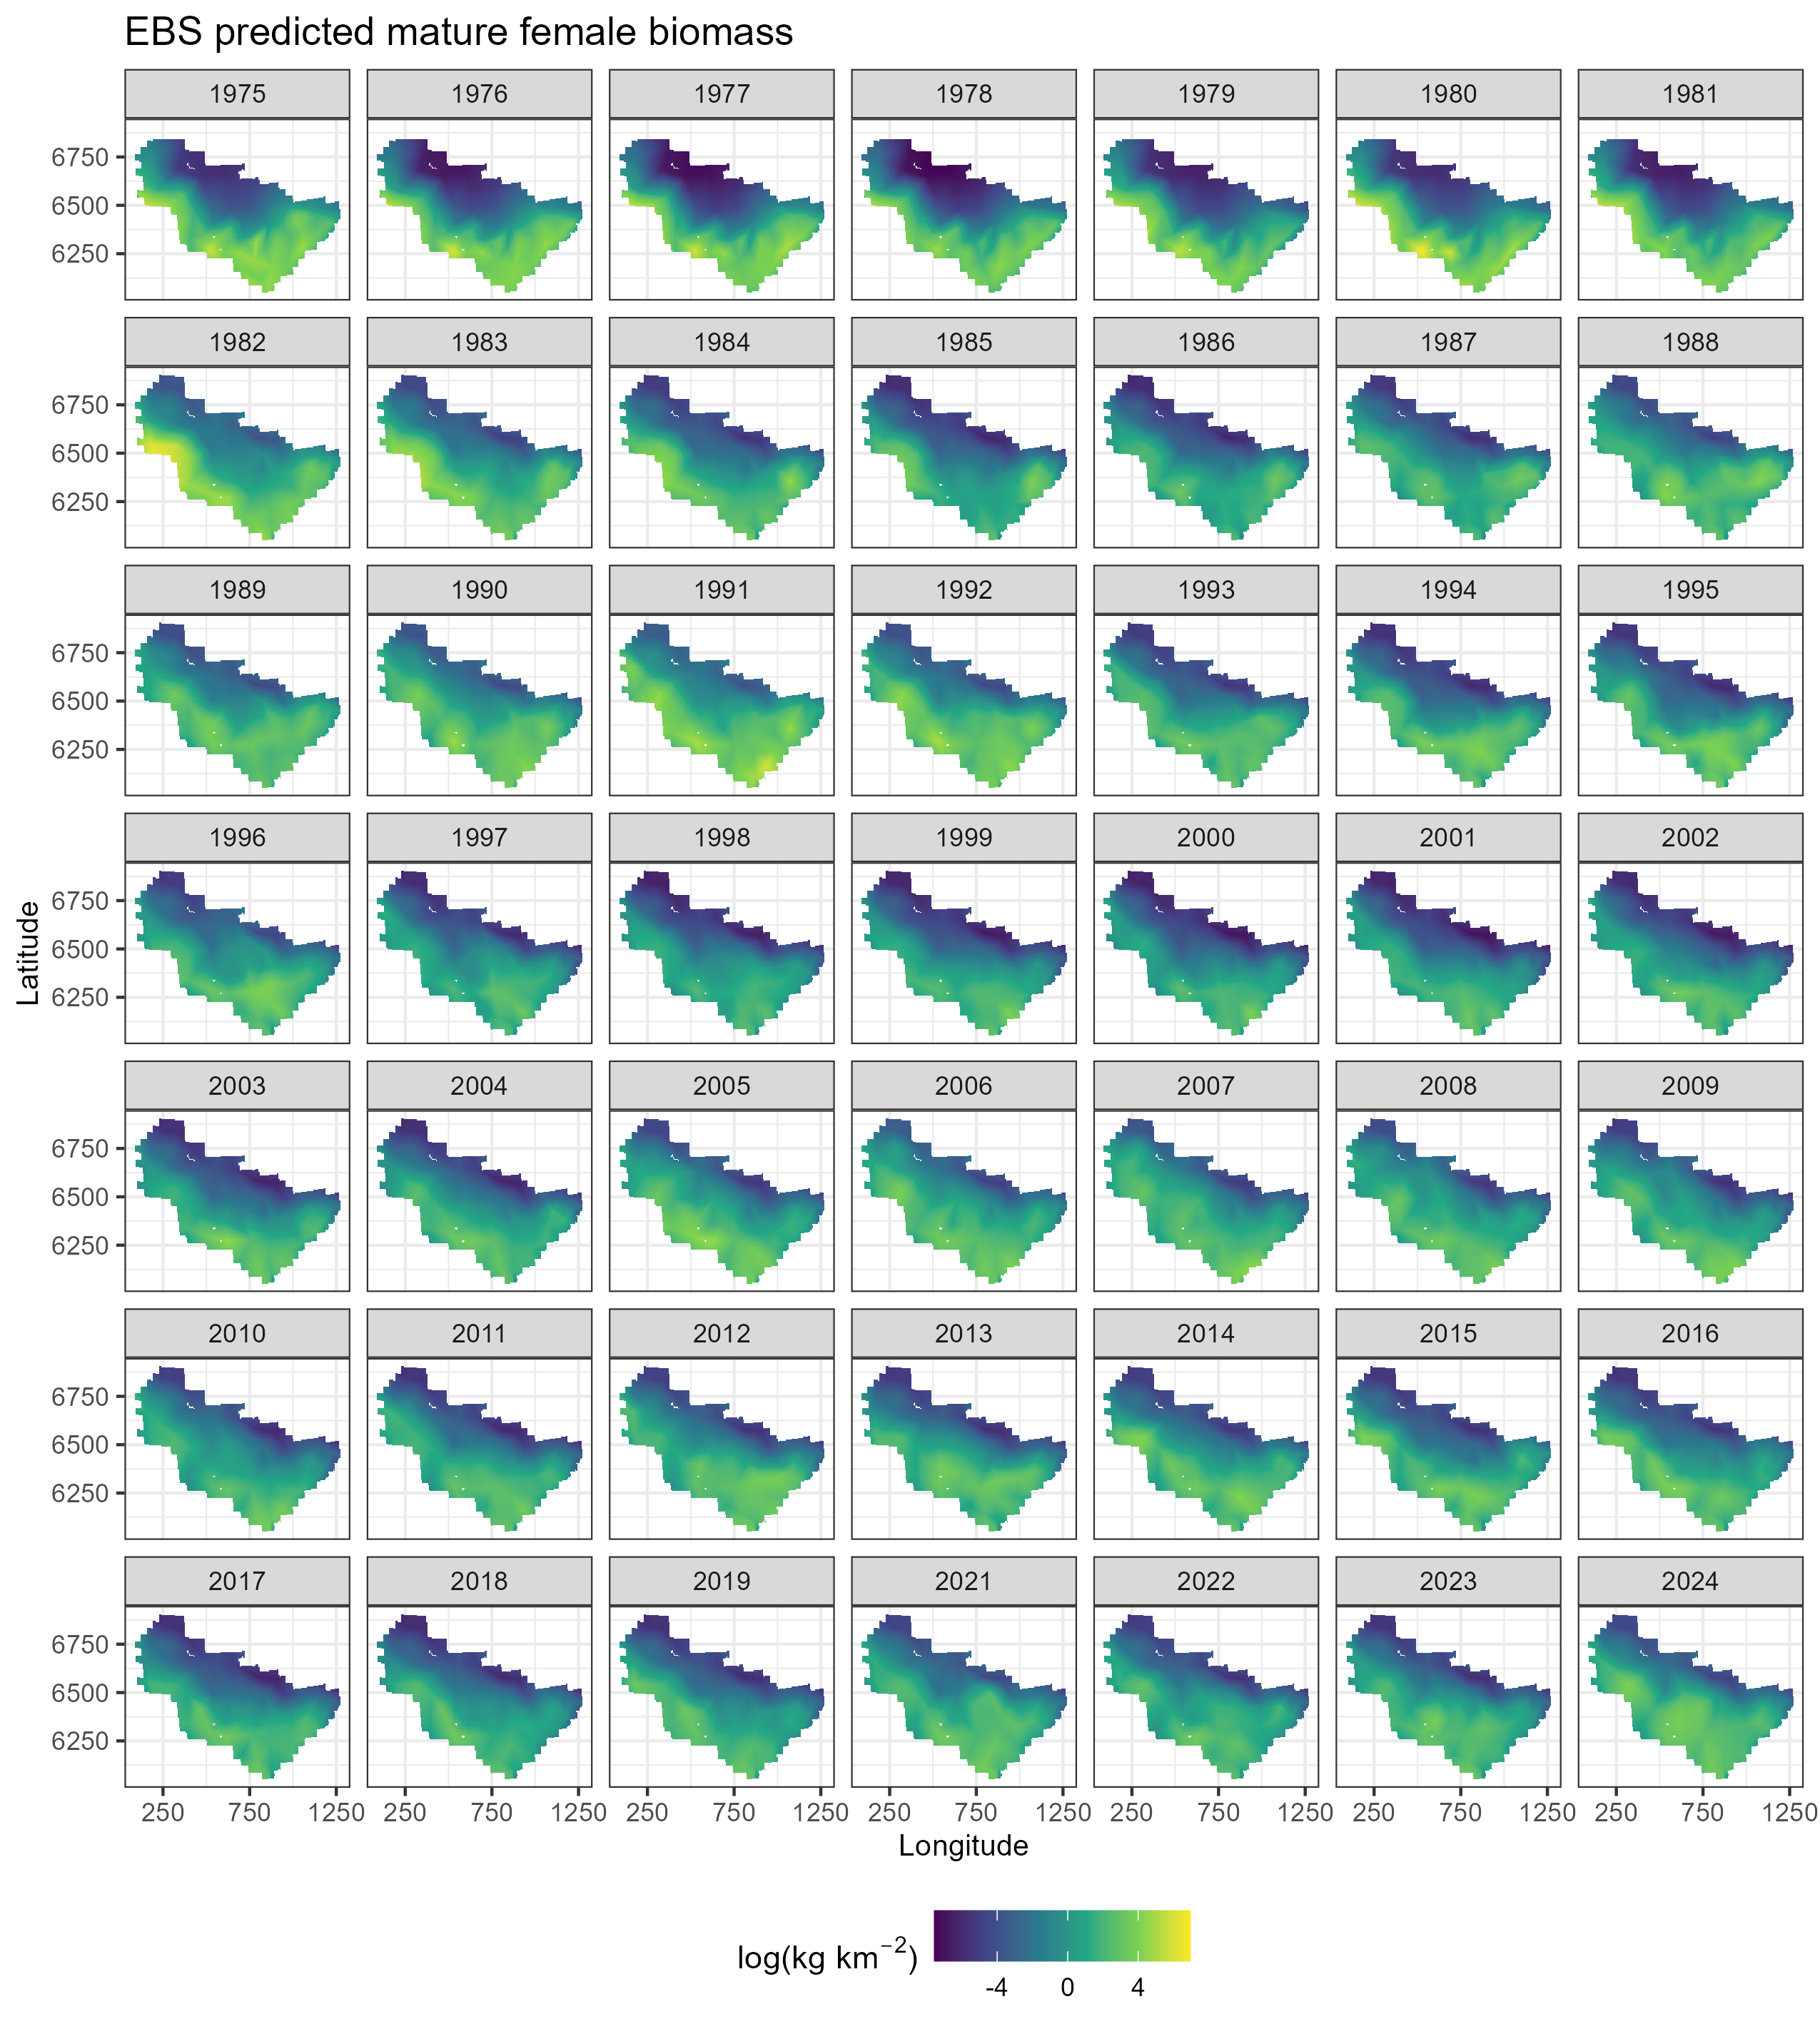
\includegraphics[width=1\linewidth,height=1\textheight]{../BAIRDI/Figures/EBS_matfem_spatbio} 

}

\caption{Spatial predictions of mature female biomass across the eastern Bering Sea using NMFS summer bottom trawl survey data before 1982 and 1982 onward with a 50-knot mesh and a delta-gamma model family. Predictions from both of these periods/models are combined in this figure.}\label{fig:spatpred-bio-50-matfem}
\end{figure}

\begin{figure}

{\centering 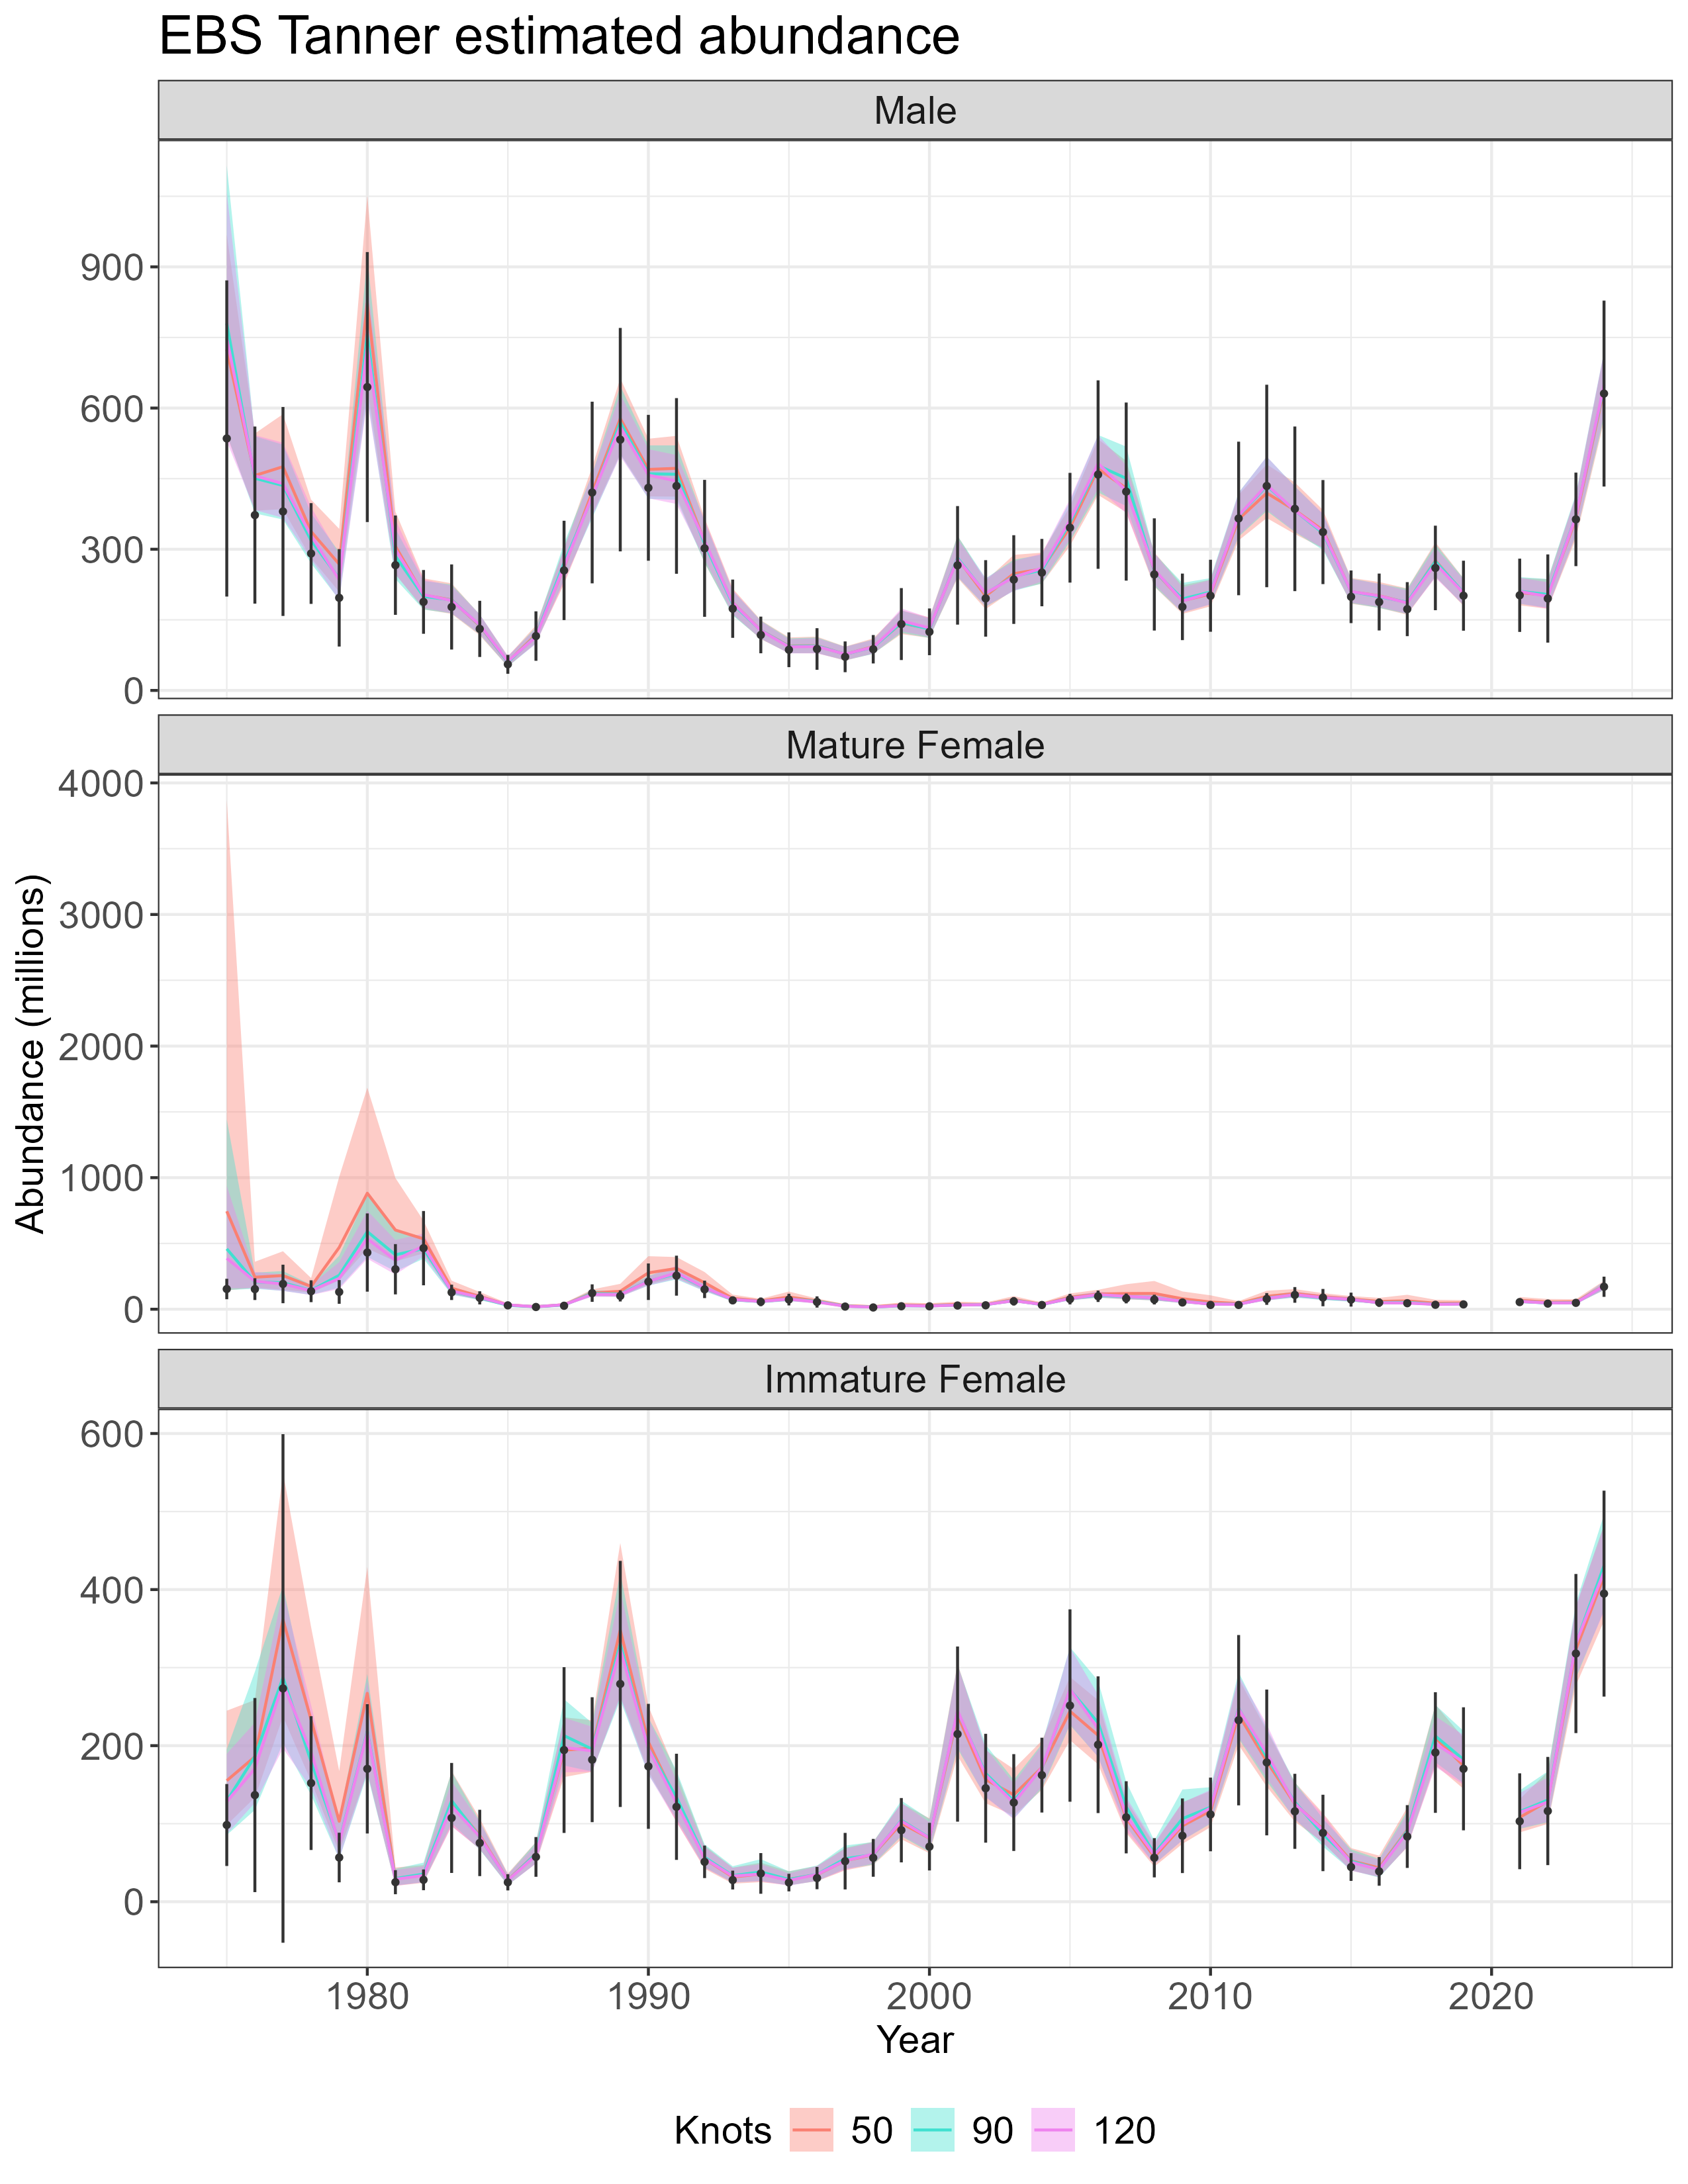
\includegraphics[width=1\linewidth,height=1\textheight]{../BAIRDI/Figures/TannerEBS.abundance.index} 

}

\caption{Estimated abundance (millions) for Tanner crab across the eastern Bering Sea. Colored lines represent abundance (±95\% CI) estimated by sdmTMB, with orange, blue, and pink denoting models fit with a 50-, 90-, and 120-knot mesh, respectively. Black points represent abundance (±95\% CI) estimated by the NMFS summer bottom trawl survey.}\label{fig:bairdi-abund-index}
\end{figure}

\begin{figure}

{\centering 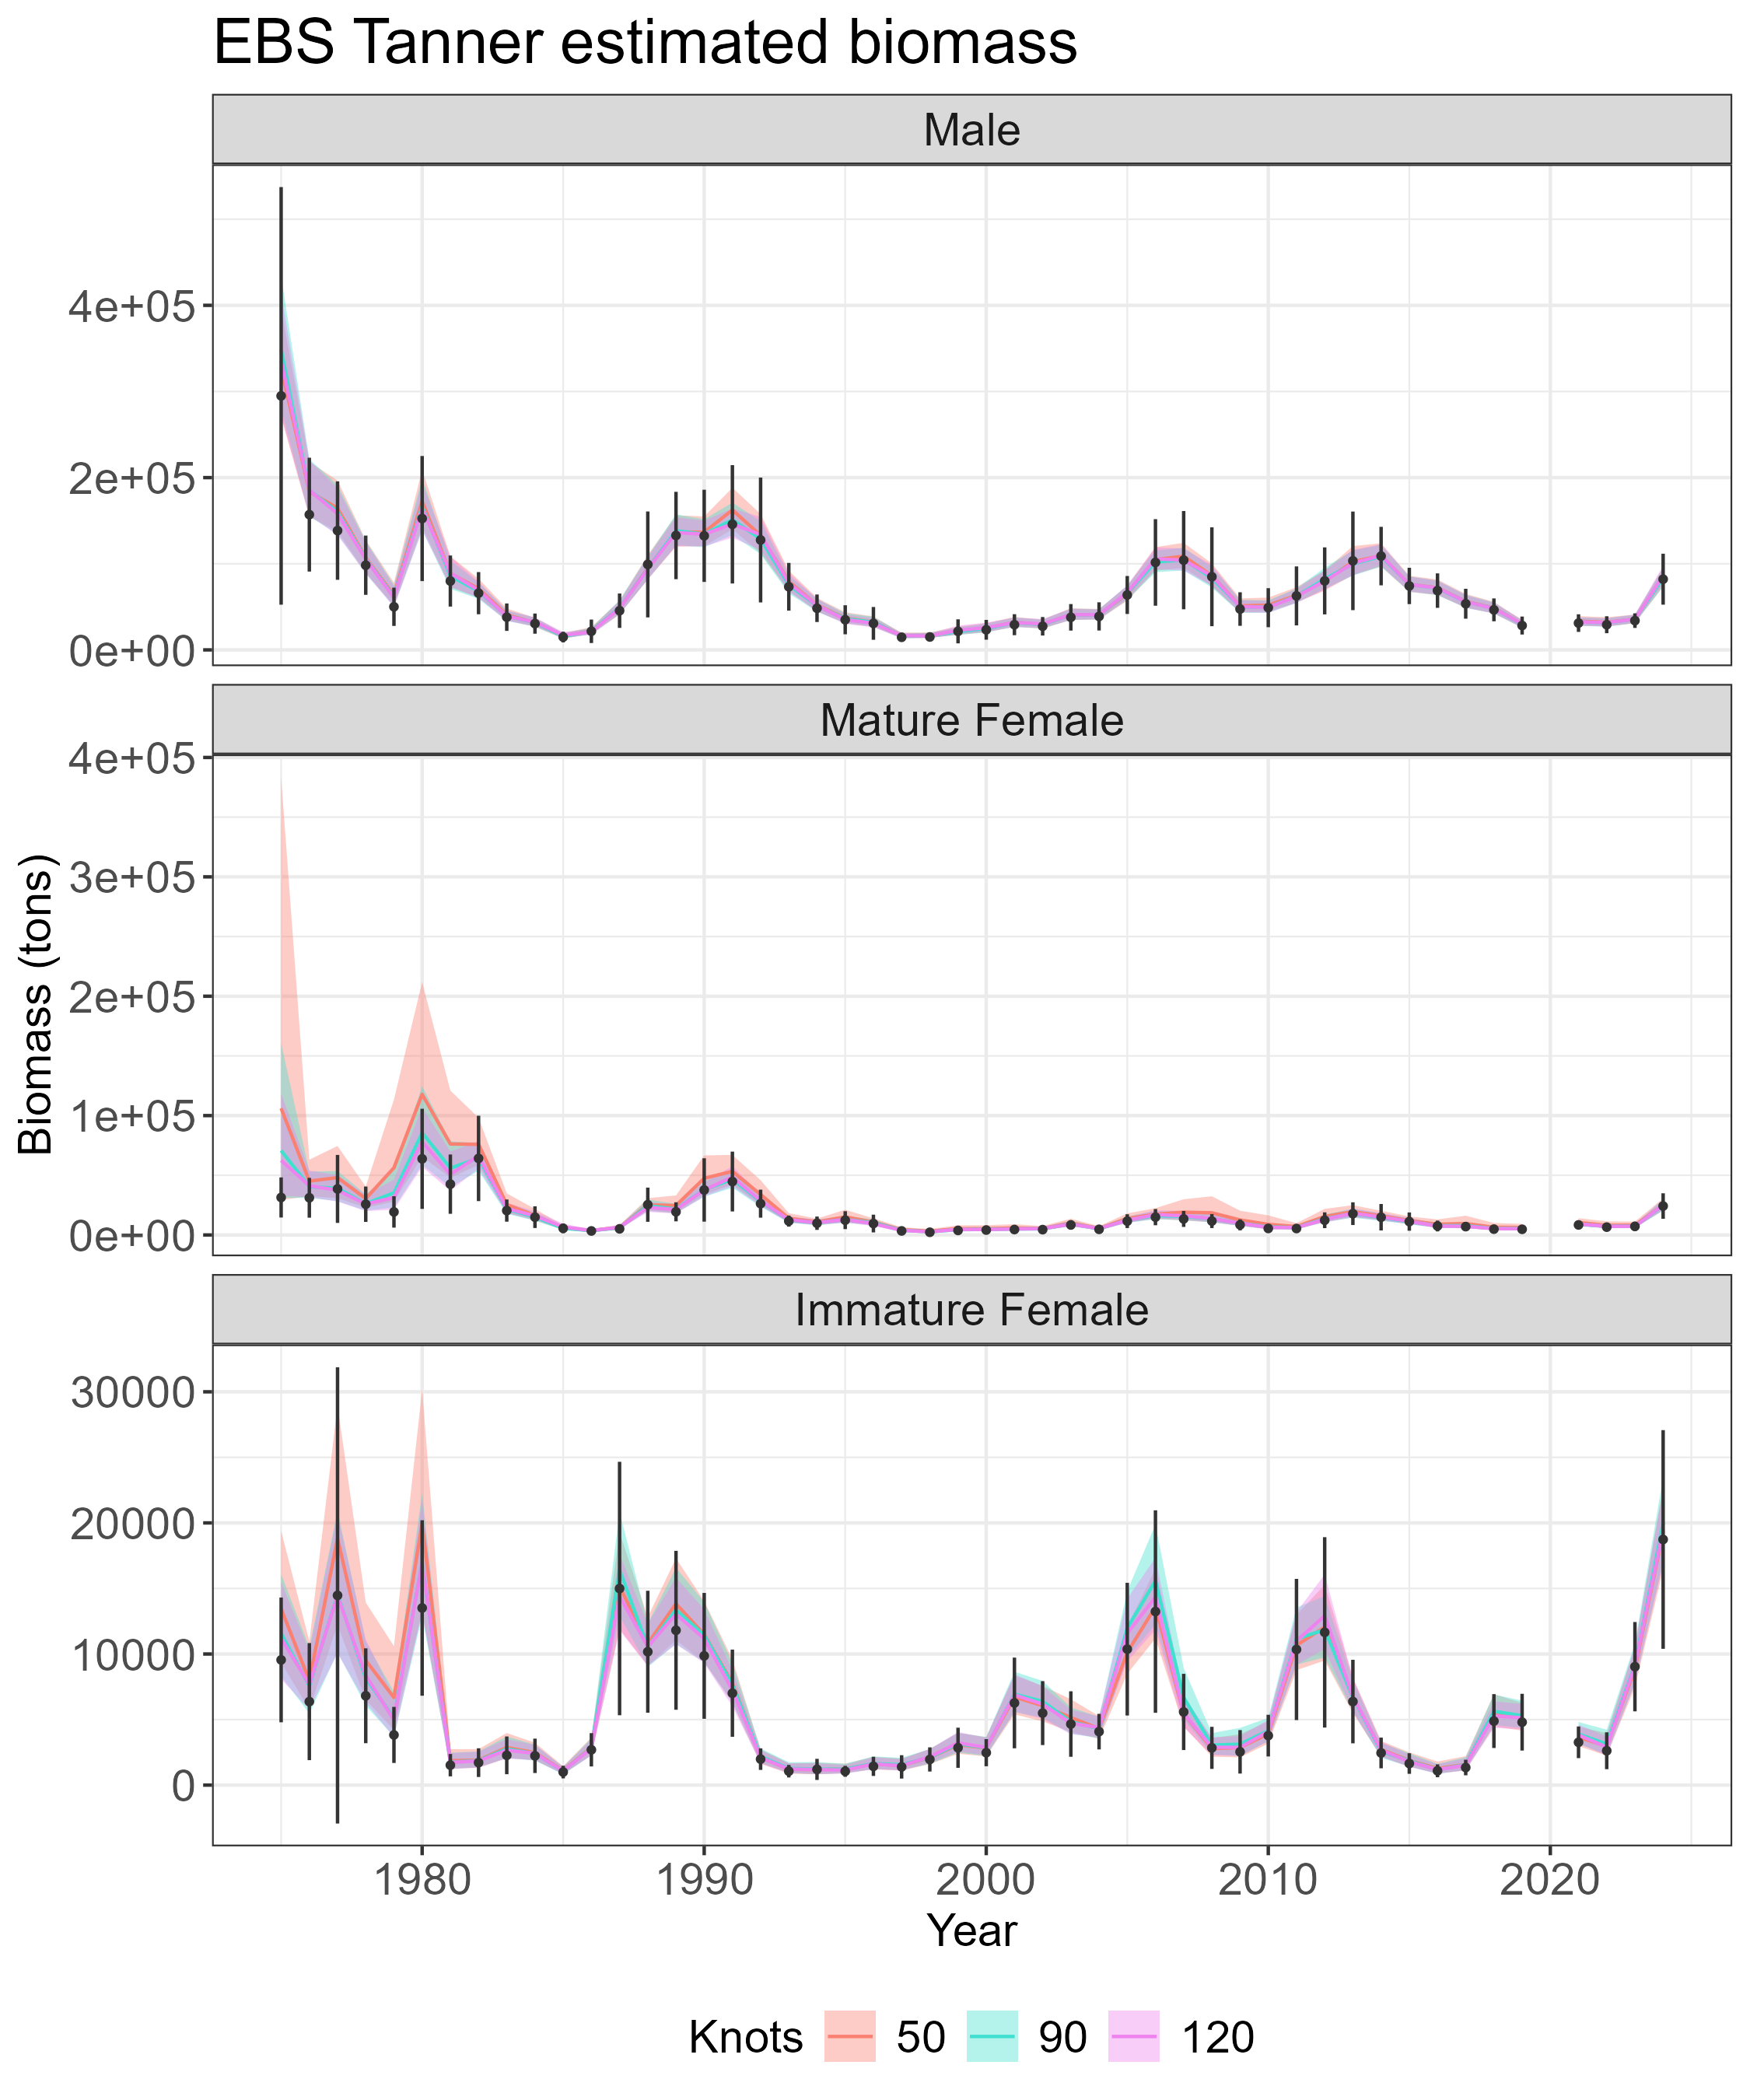
\includegraphics[width=1\linewidth,height=1\textheight]{../BAIRDI/Figures/TannerEBS.biomass.index} 

}

\caption{Estimated biomass (tons) for eastern Bering Sea Tanner crab across the eastern Bering Sea. Colored lines represent abundance (±95\% CI) estimated by sdmTMB, with orange, blue, and pink denoting models fit with a 50-, 90-, and 120-knot mesh, respectively. Black points represent biomass (±95\% CI) estimated by the NMFS summer bottom trawl survey.}\label{fig:bairdi-bio-index}
\end{figure}

\begin{figure}

{\centering 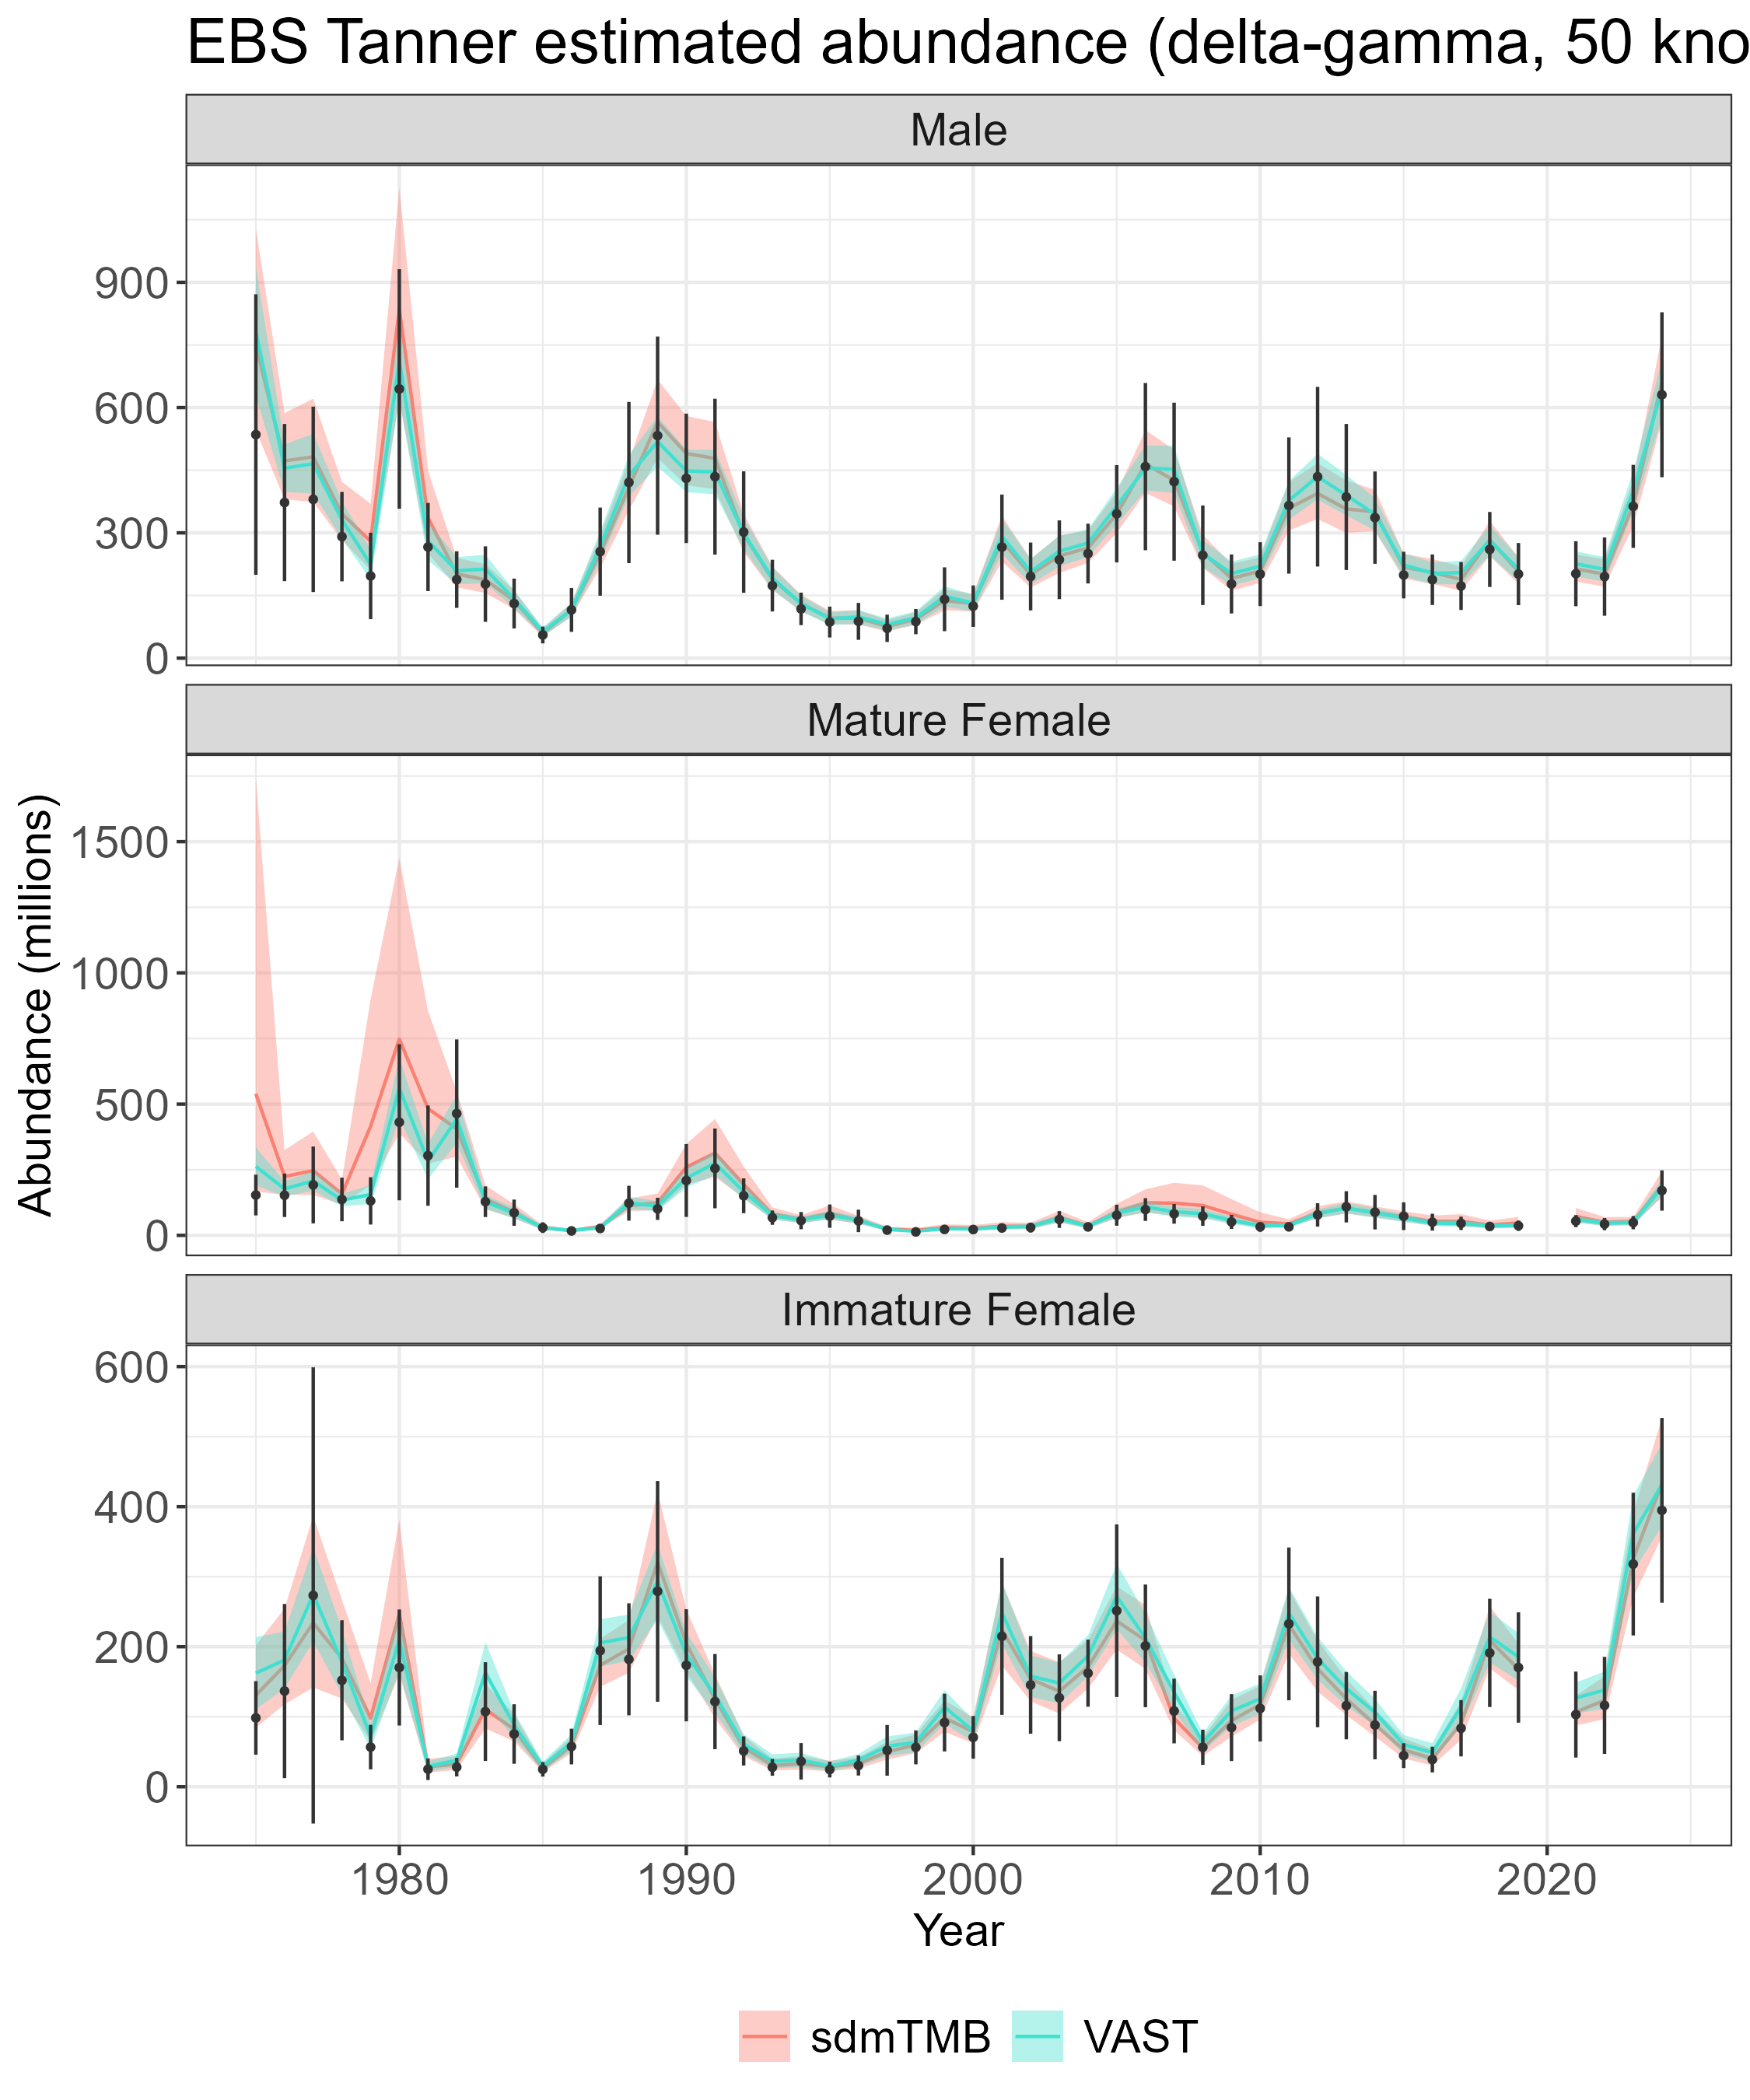
\includegraphics[width=1\linewidth,height=1\textheight]{../BAIRDI/Figures/TannerEBS.abundance.sdmTMBVASTindex} 

}

\caption{Estimated abundance (millions; ±95\% CI) for eastern Bering Sea Tanner crab predicted using sdmTMB (pink) and VAST (blue). Both algorithms fit models using a delta-gamma family at 50 knots. Black points represent abundance (±95\% CI) estimated by the NMFS summer bottom trawl survey.}\label{fig:EBSbairdi-abund-compare}
\end{figure}

\begin{figure}

{\centering 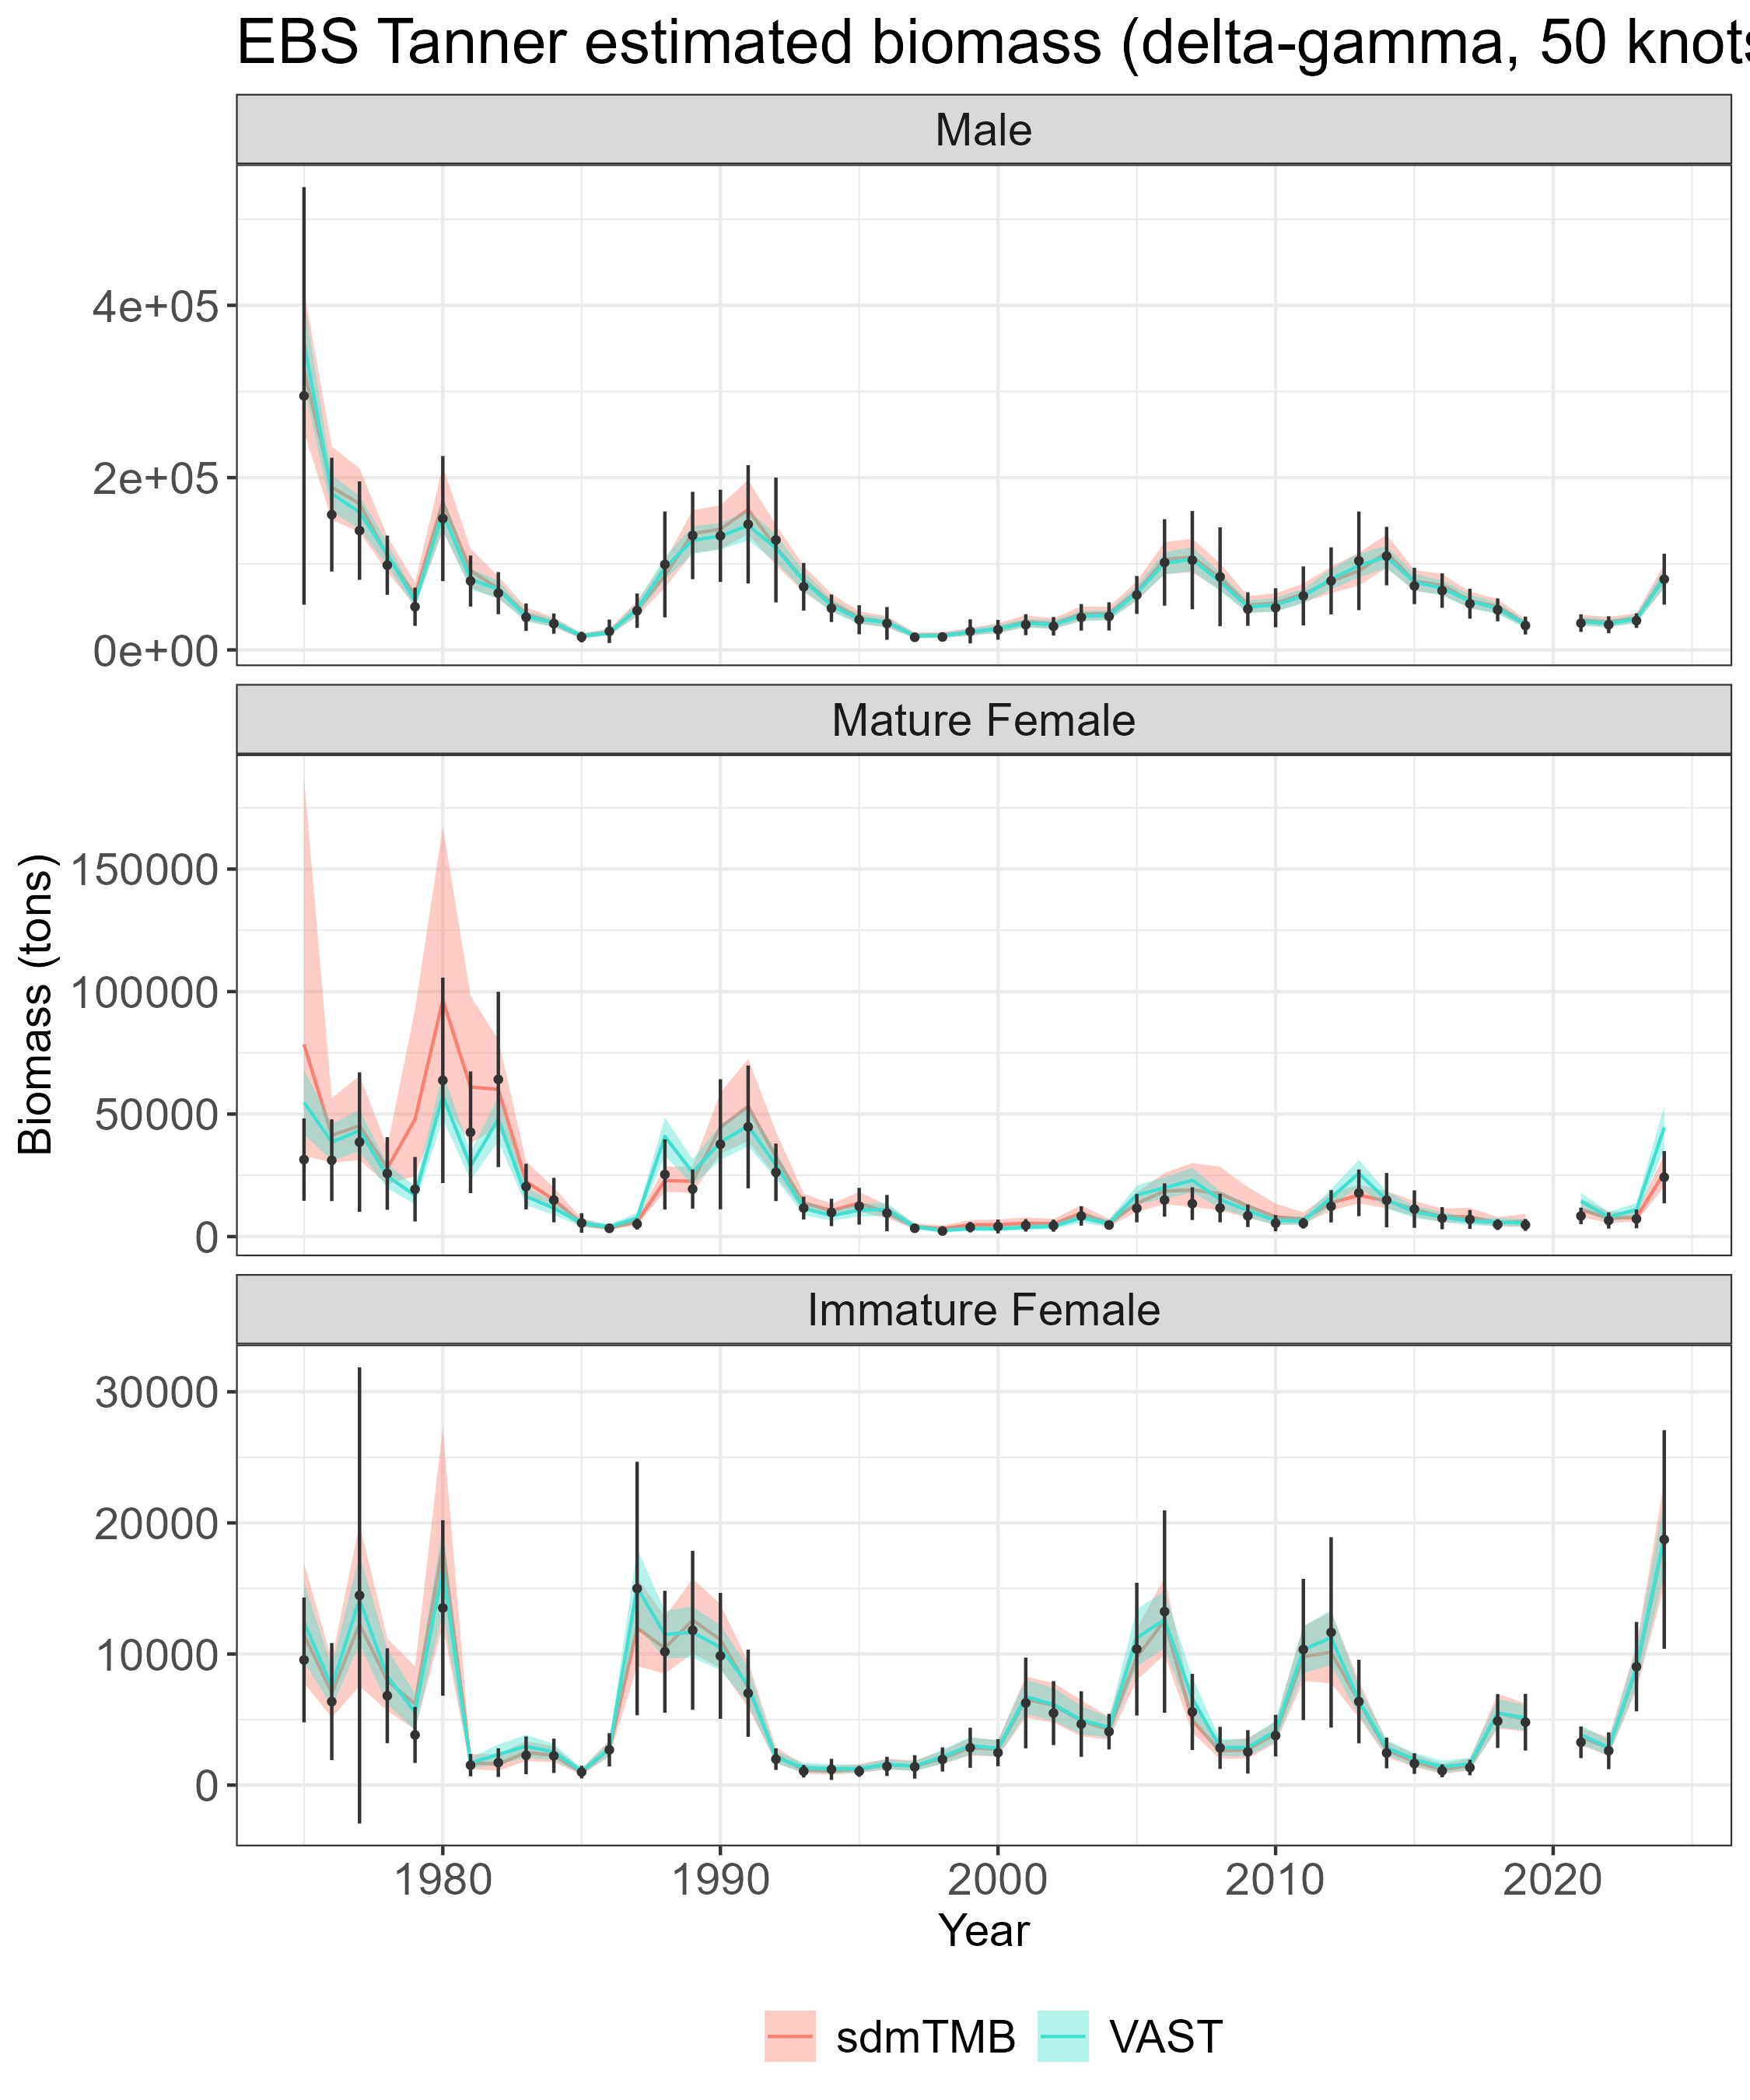
\includegraphics[width=1\linewidth,height=1\textheight]{../BAIRDI/Figures/TannerEBS.biomass.sdmTMBVASTindex} 

}

\caption{Estimated biomass (tons; ±95\% CI) for eastern Bering Sea Tanner crab predicted using sdmTMB (pink) and VAST (blue). Both algorithms fit models using a delta-gamma family at 50 knots. Black points represent abundance (±95\% CI) estimated by the NMFS summer bottom trawl survey.}\label{fig:EBSbairdi-bio-compare}
\end{figure}

\pagebreak
\begin{figure}

{\centering 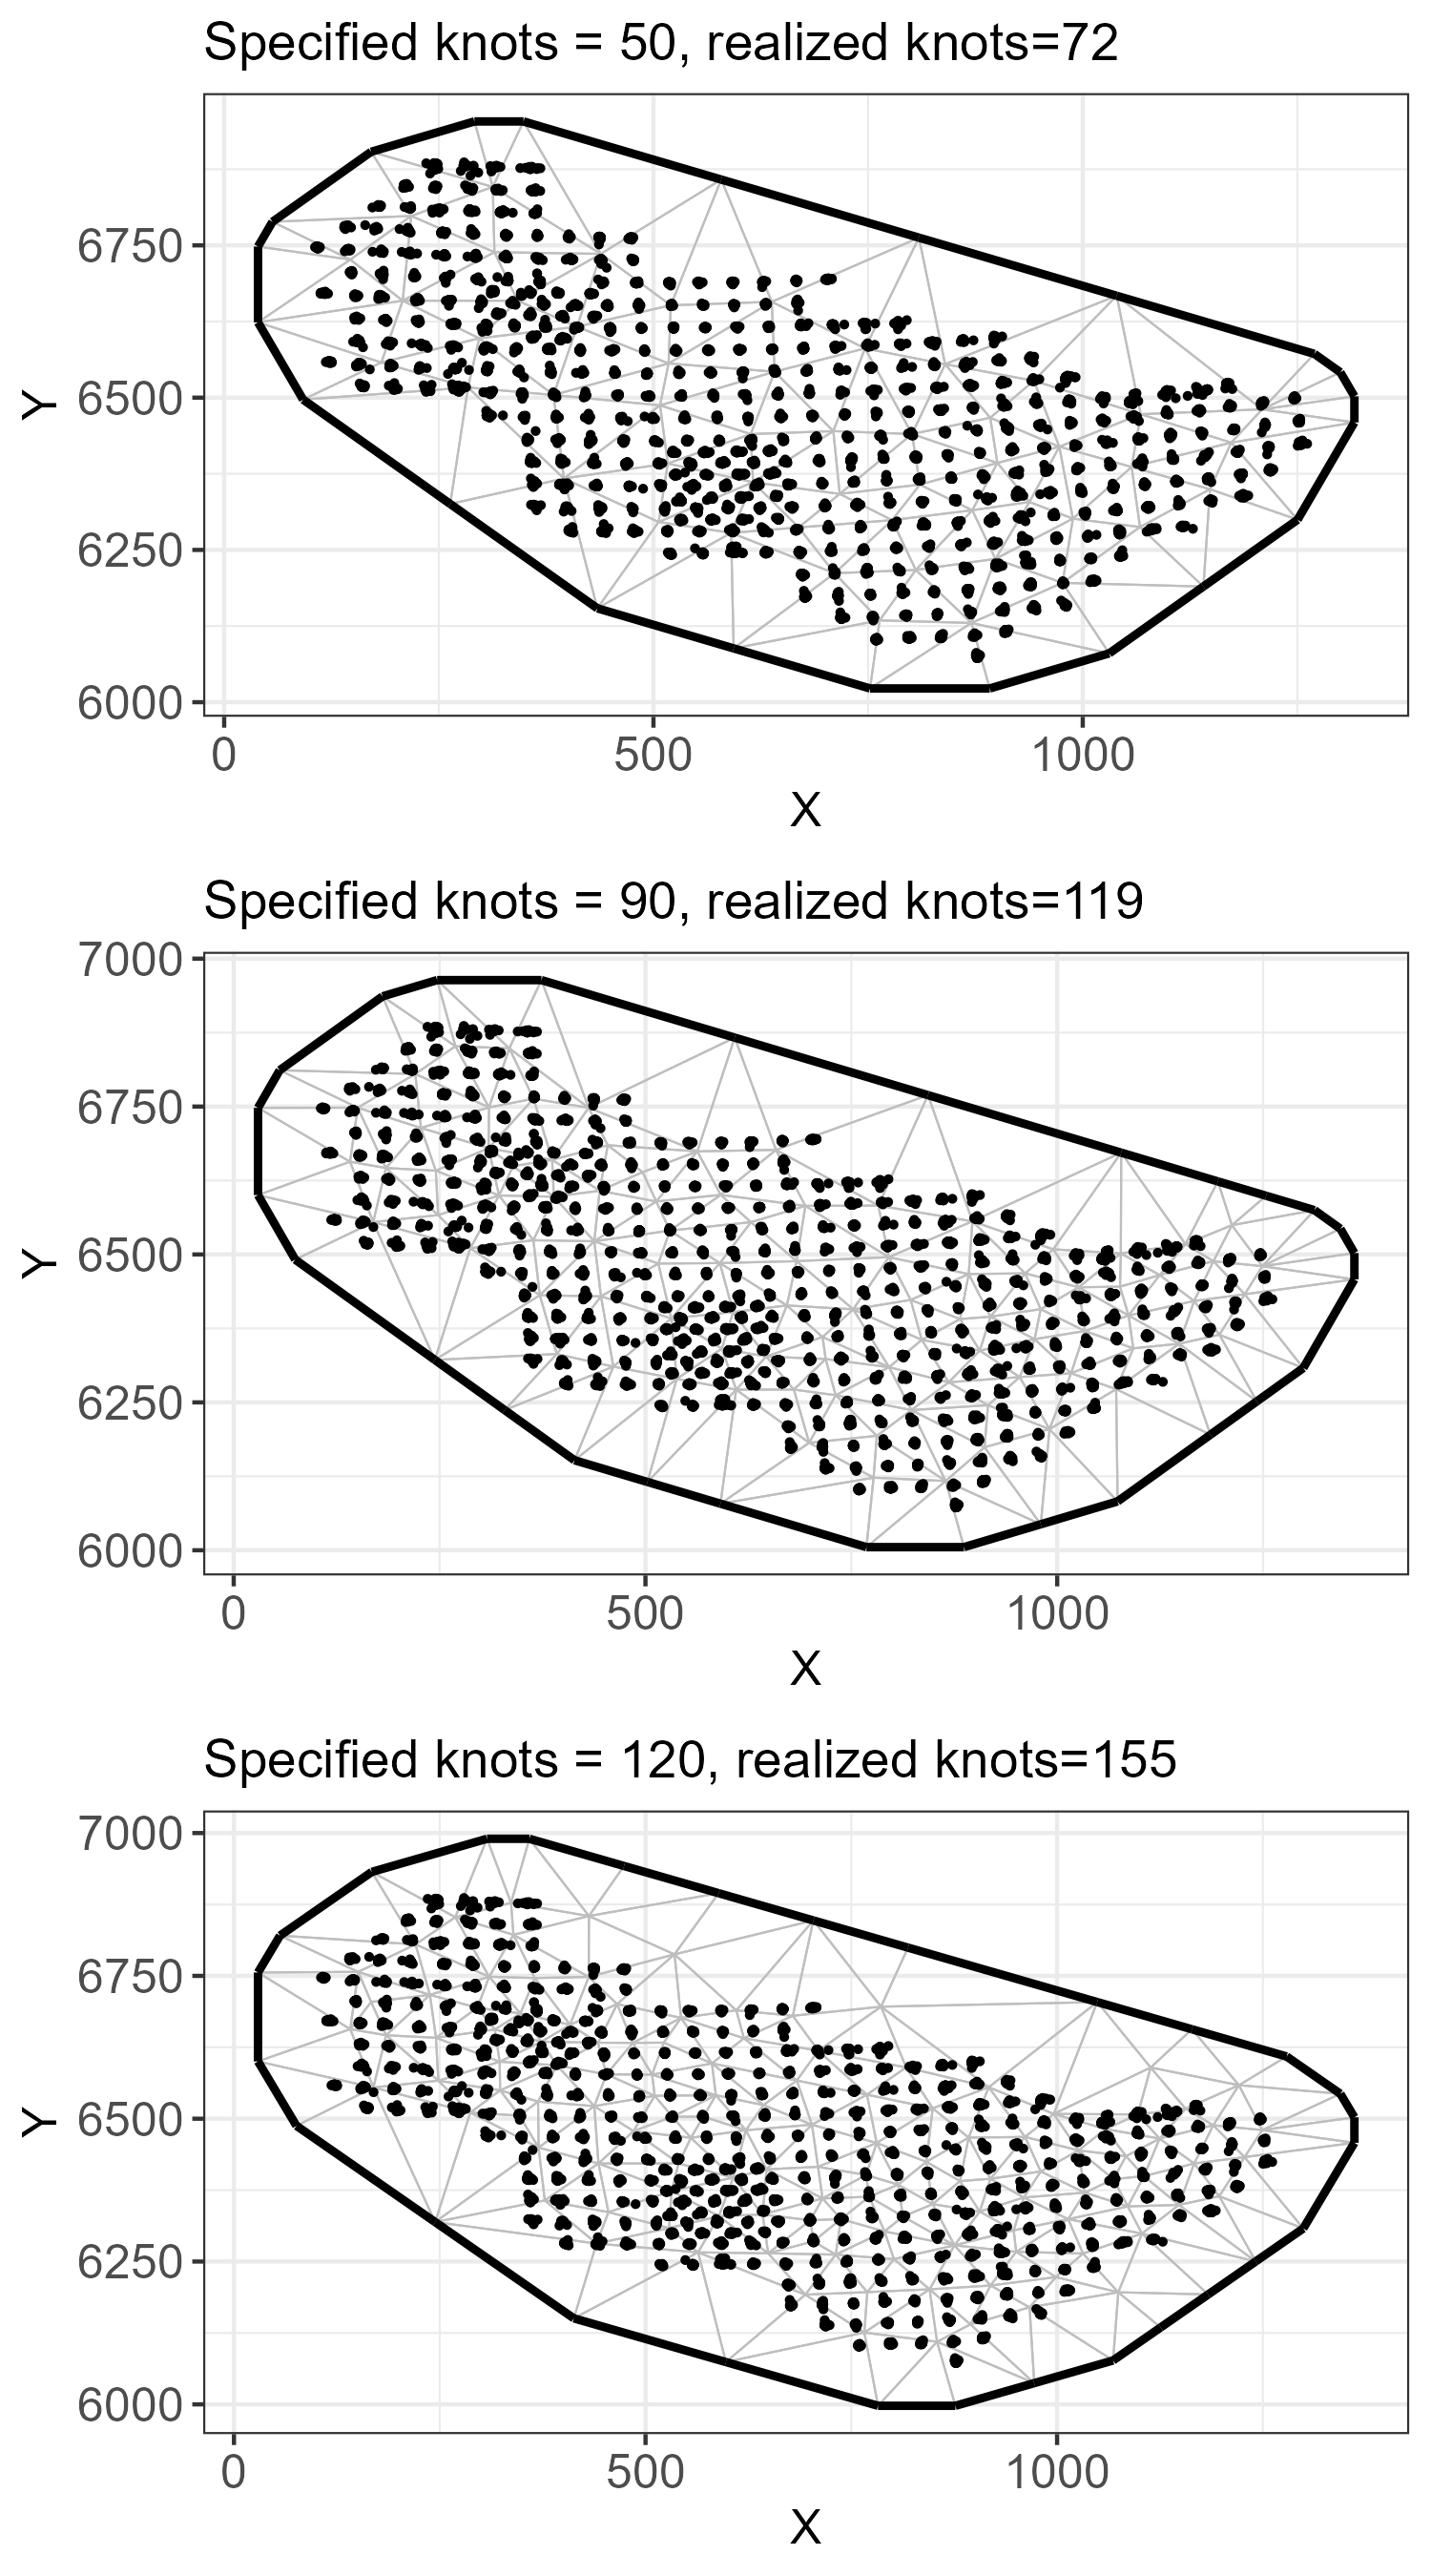
\includegraphics[width=0.75\linewidth,height=0.75\textheight]{../SNOW/Figures/snow_EBS_mesh} 

}

\caption{Eastern Bering Sea spatial mesh with 50-, 90-, and 120- knots used for fitting snow crab spatial models. Points represent observations and vertices represent knot locations. The title denotes the realized number of knots after mesh generation.}\label{fig:snow-EBS-mesh}
\end{figure}

\begin{figure}

{\centering 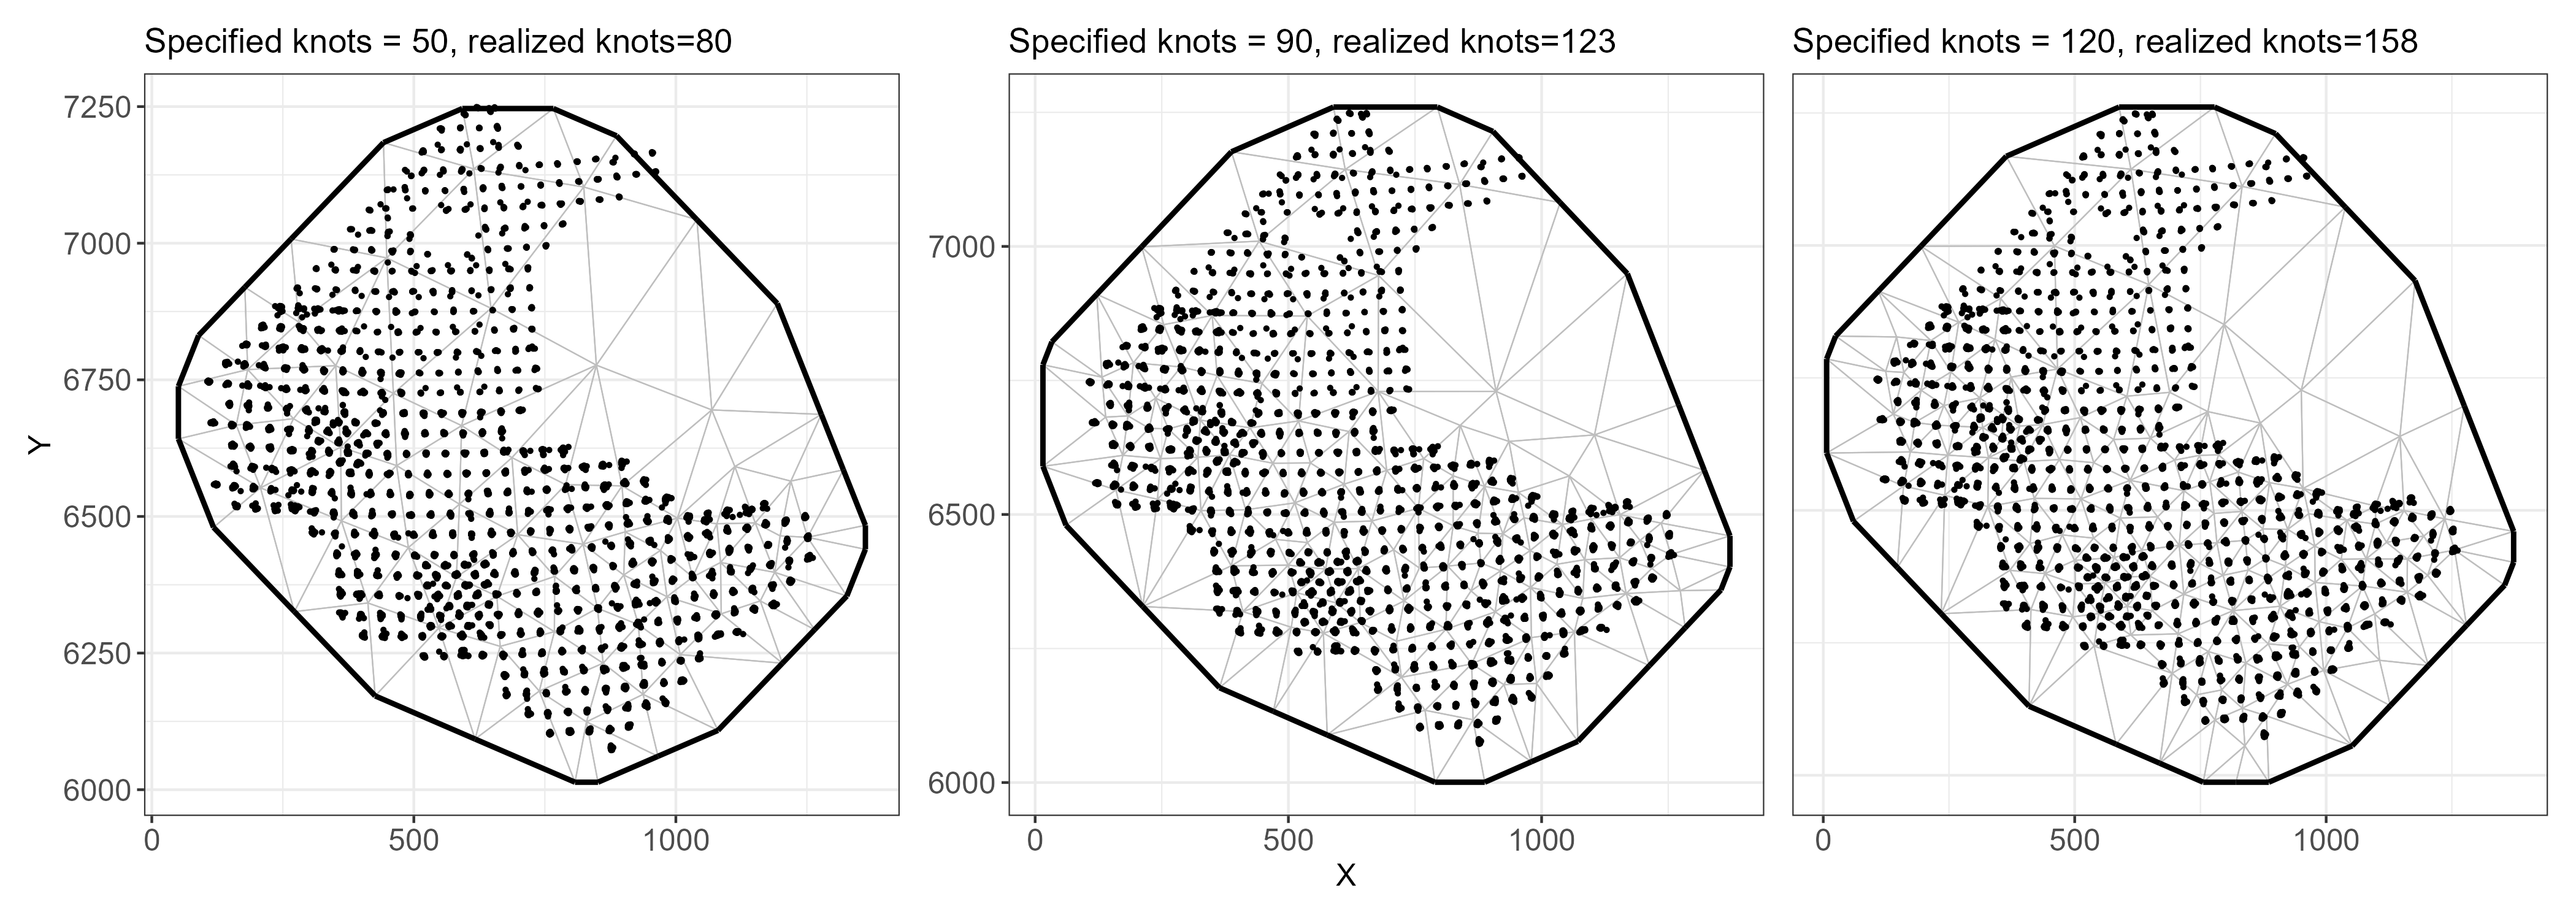
\includegraphics[width=0.75\linewidth,height=0.75\textheight]{../SNOW/Figures/snow_EBS-NBS_mesh} 

}

\caption{Eastern Bering Sea and northern Bering Sea spatial mesh with 50-, 90-, and 120- knots used for fitting snow crab spatial models. Points represent observations and vertices represent knot locations. The title denotes the realized number of knots after mesh generation.}\label{fig:snow-NBS-mesh}
\end{figure}

\begin{figure}

{\centering 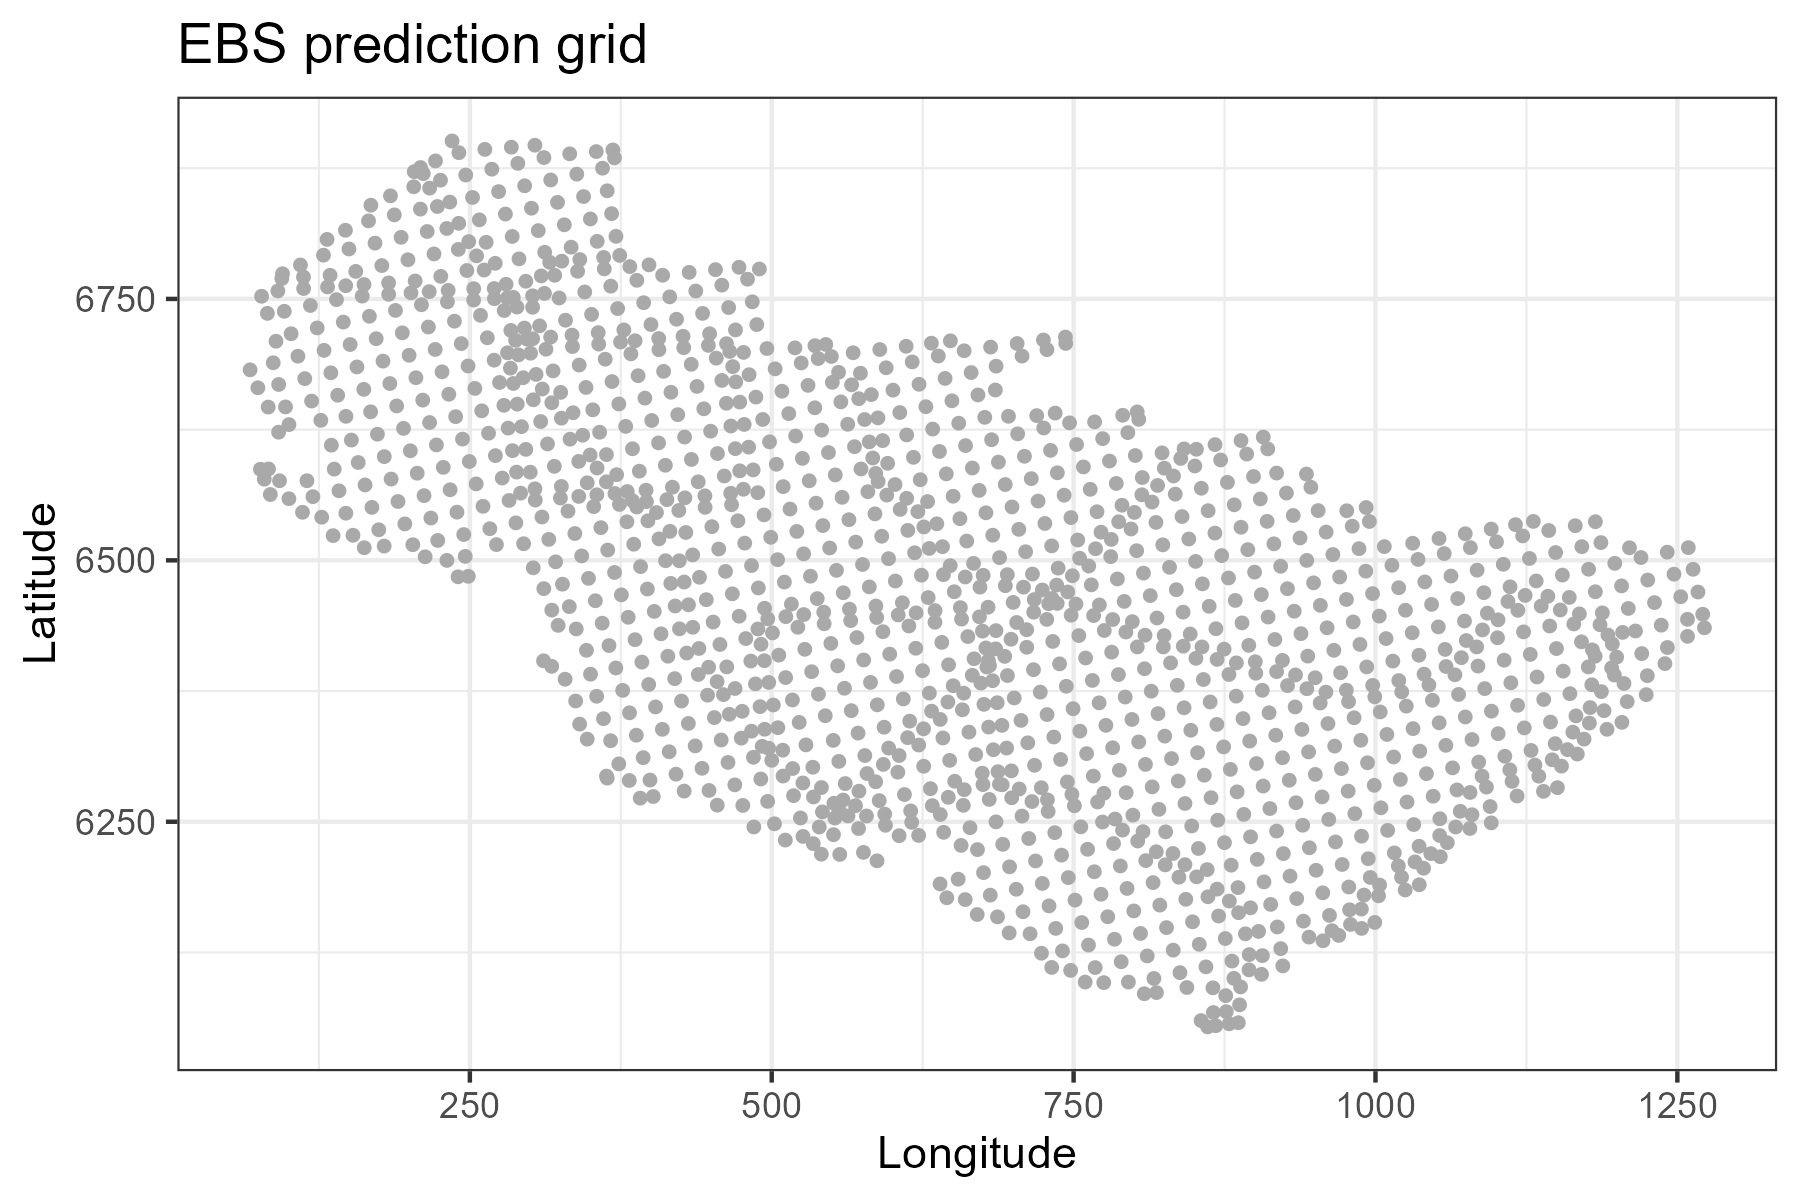
\includegraphics[width=6in]{../SNOW/Figures/EBS_predgrid} 

}

\caption{Eastern Bering Sea prediction grid used for snow crab spatial abundance and biomass predictions. Spatial resolution is 41km$^2$ and does not include land.}\label{fig:snow-EBS-grid}
\end{figure}

\begin{figure}

{\centering 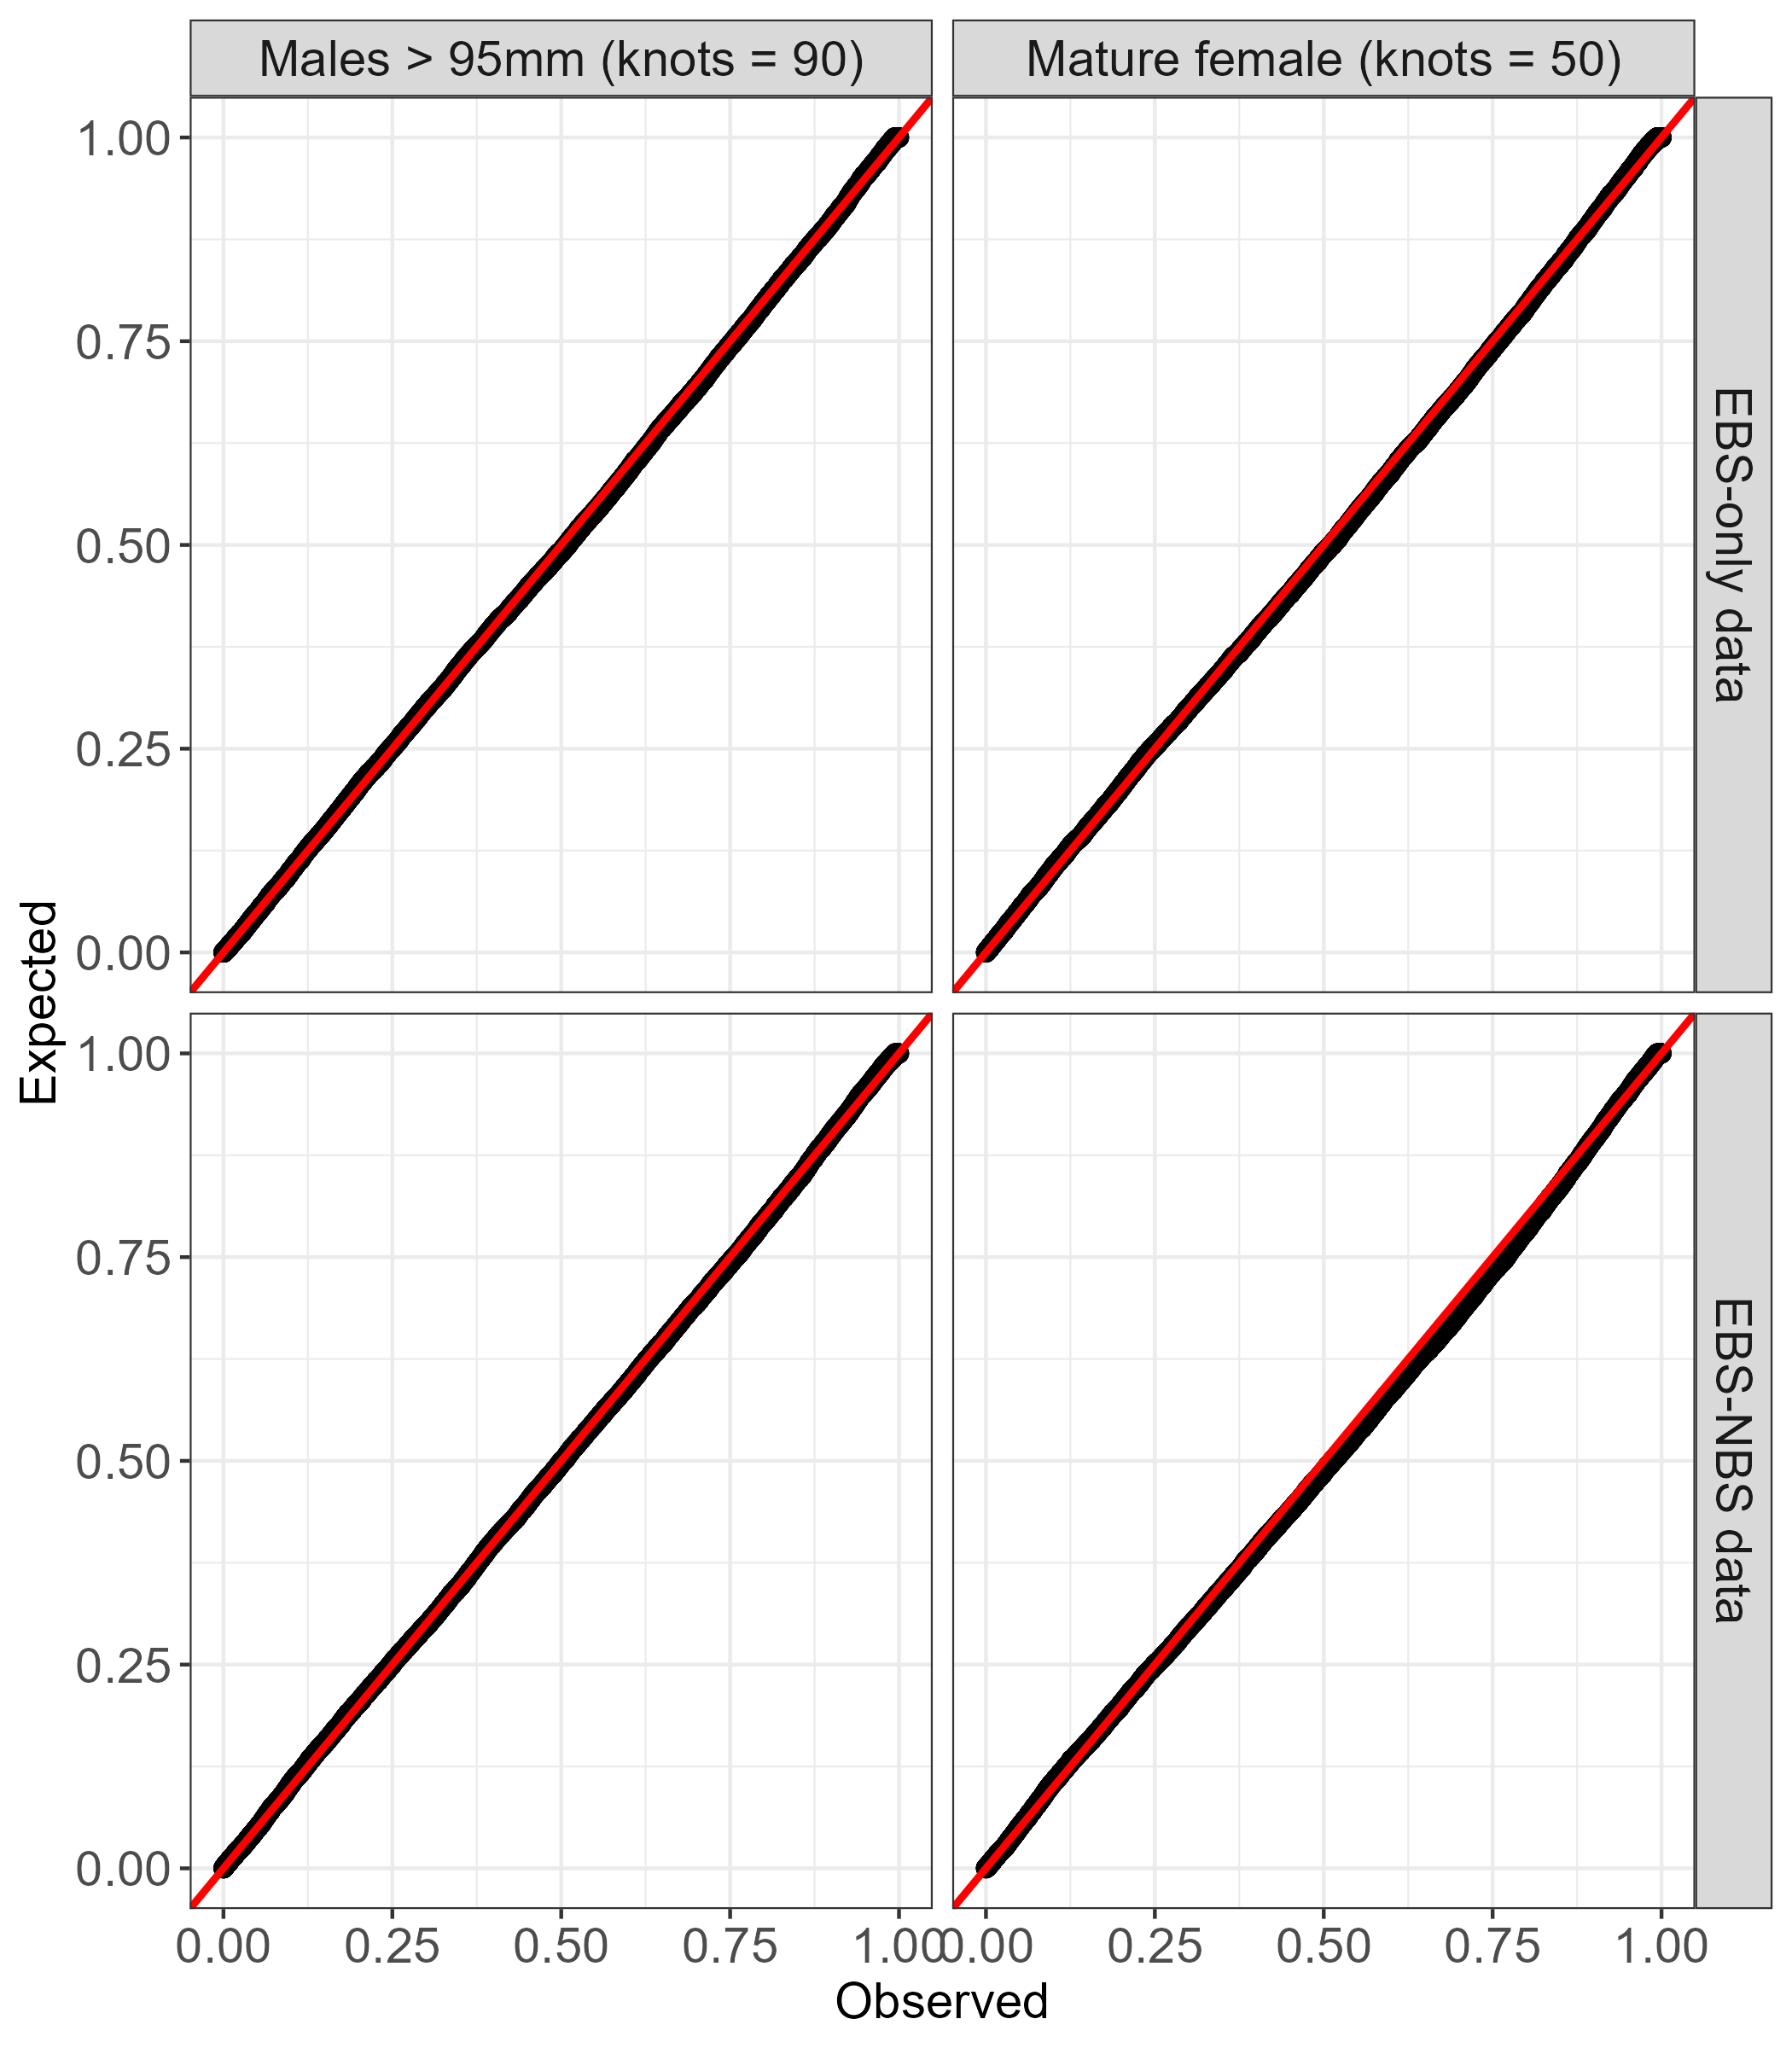
\includegraphics[width=1\linewidth,height=1\textheight]{../SNOW/Figures/DHARMa_EBSNBS_QQplot} 

}

\caption{Q-Q plot of DHARMa residuals for male (>95mm) biomass and mature female snow crab models fit with NMFS summer bottom trawl survey data from the EBS-only (top row) and EBS-NBS data combined using a delta-gamma model family and 90 knots and 50 knots in the model mesh for males and mature females, respectively.}\label{fig:snow-DHARMa-QQ-EBSNBS}
\end{figure}

\begin{figure}

{\centering 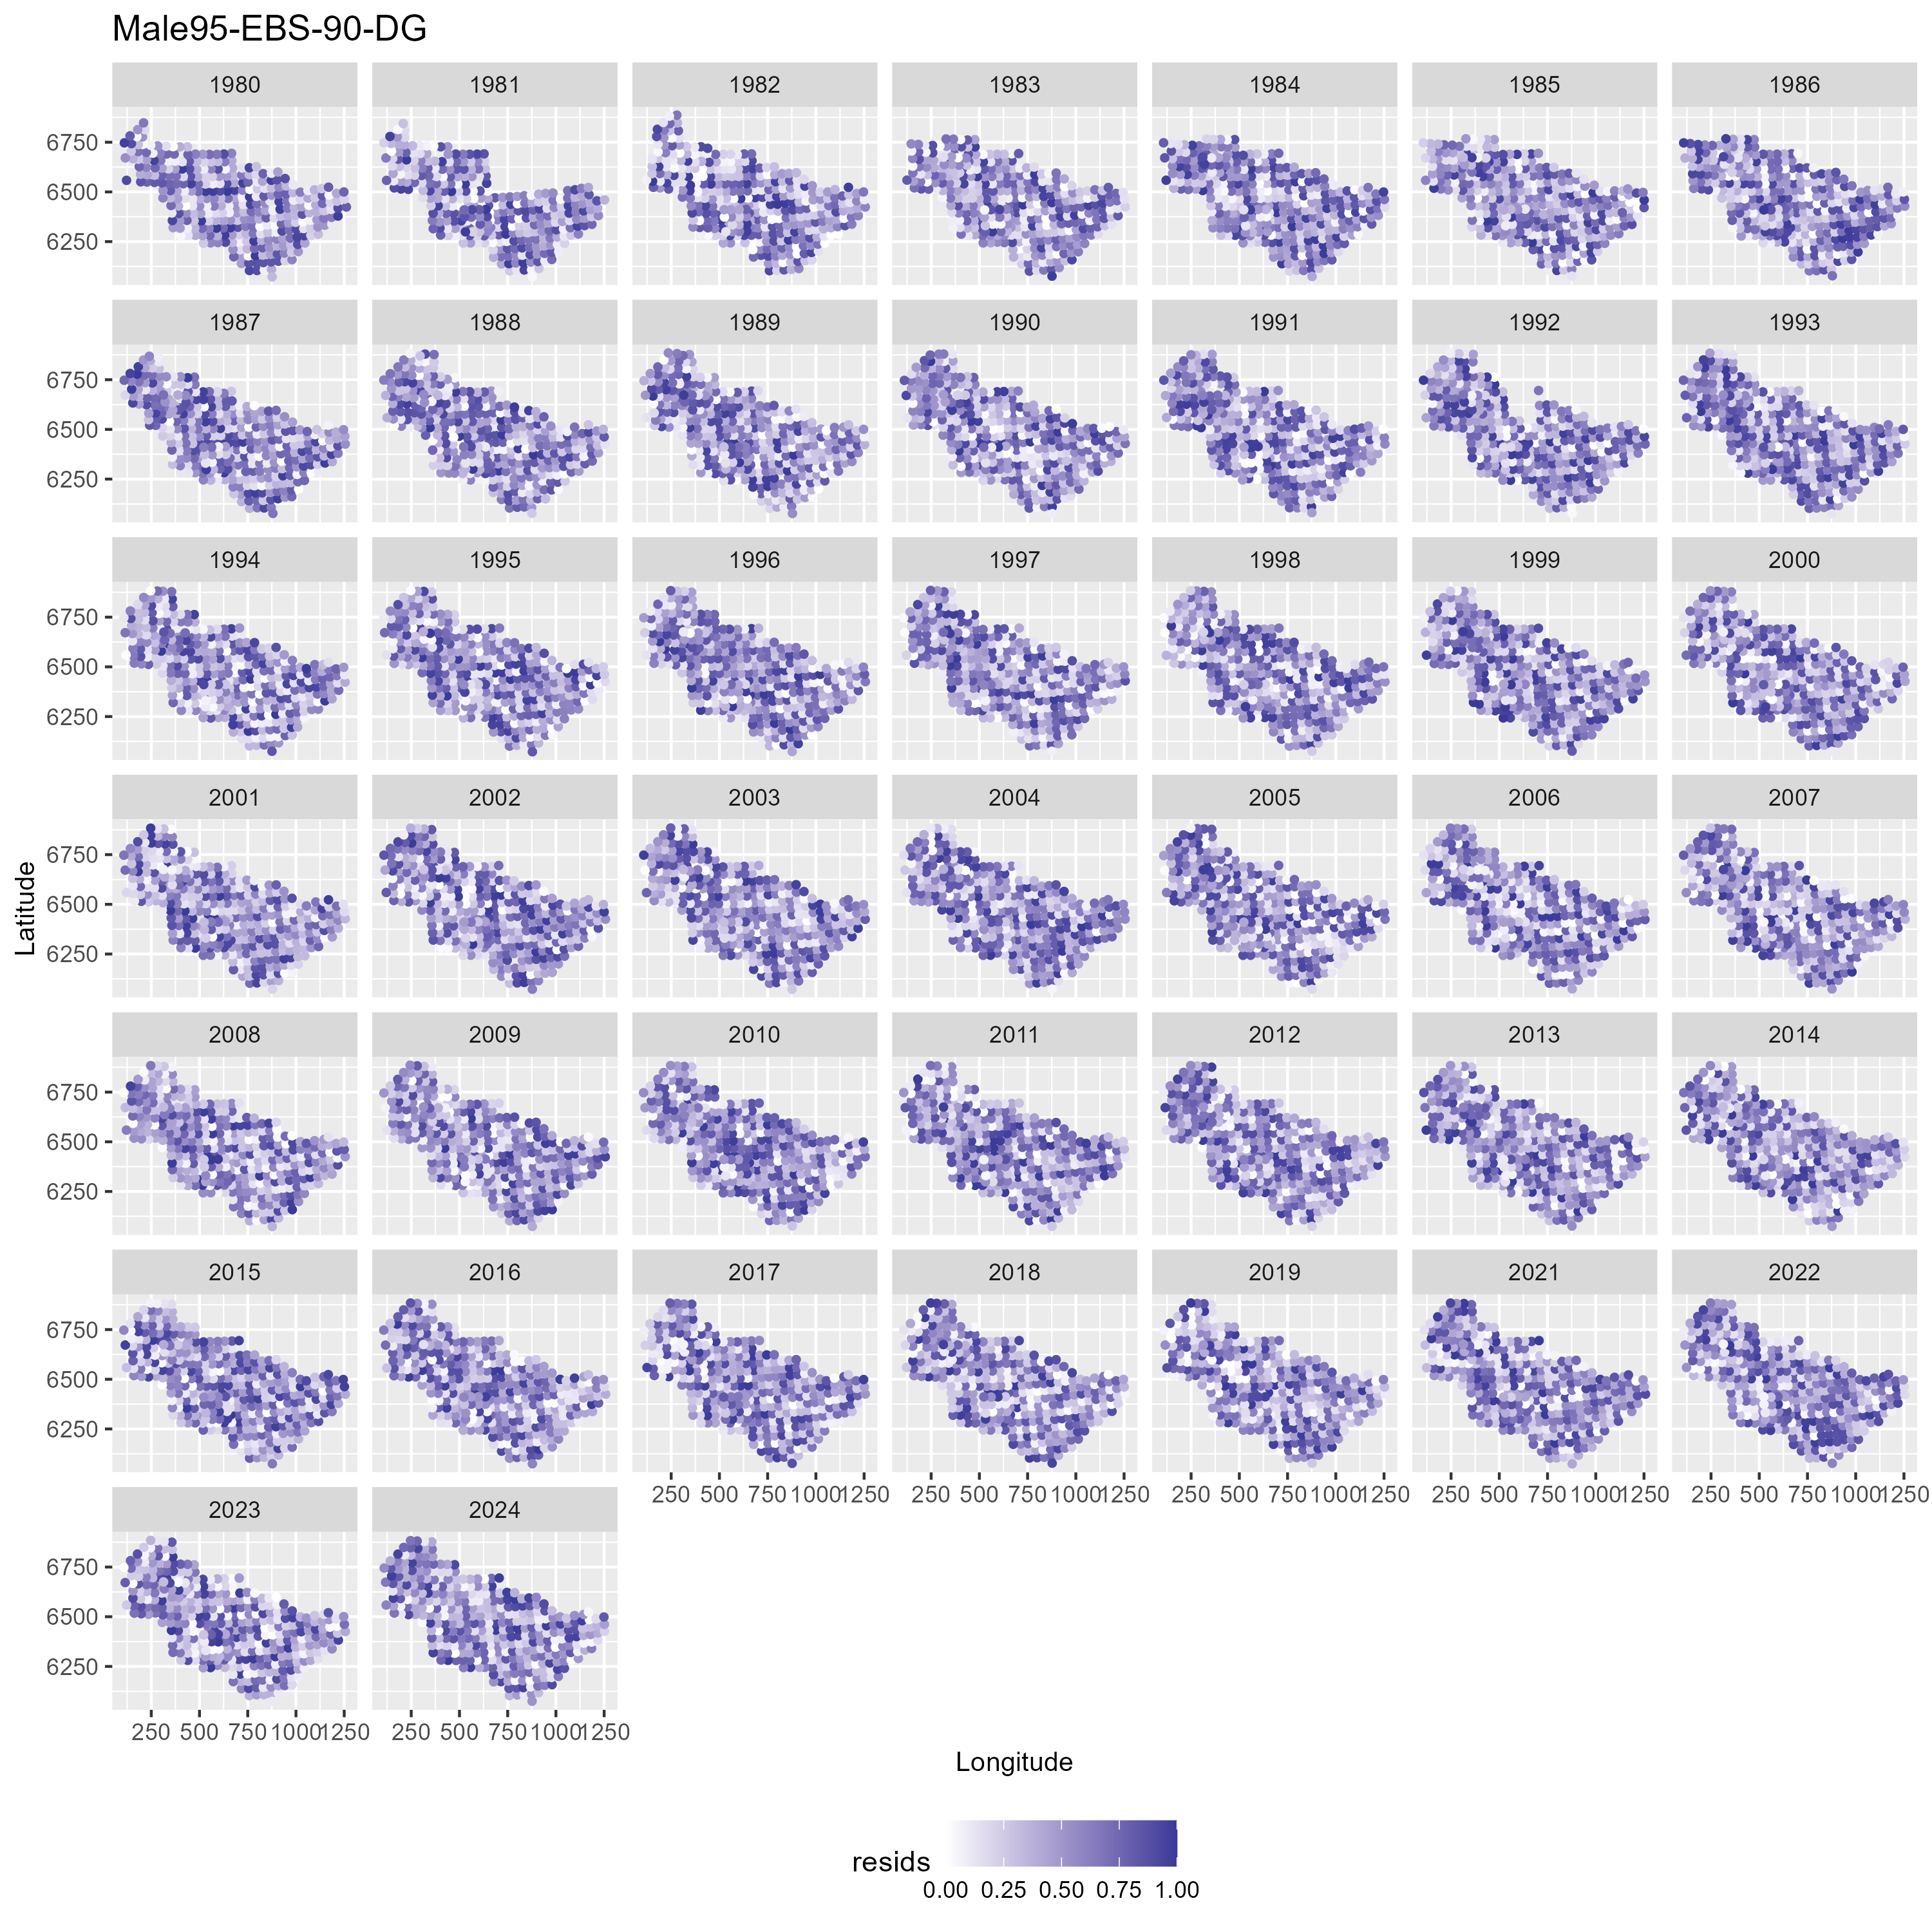
\includegraphics[width=1\linewidth,height=1\textheight]{../SNOW/Figures/DHARMa_Male95-EBS-90-DG_SPATIAL} 

}

\caption{Spatial plot of DHARMa residuals for male (> 95mm) snow crab biomass models fit using NMFS summer bottom trawl survey data from the EBS only with a 90-knot mesh and a delta-gamma model family.}\label{fig:snow-DHARMa-spat-90-male95-EBS}
\end{figure}

\begin{figure}

{\centering 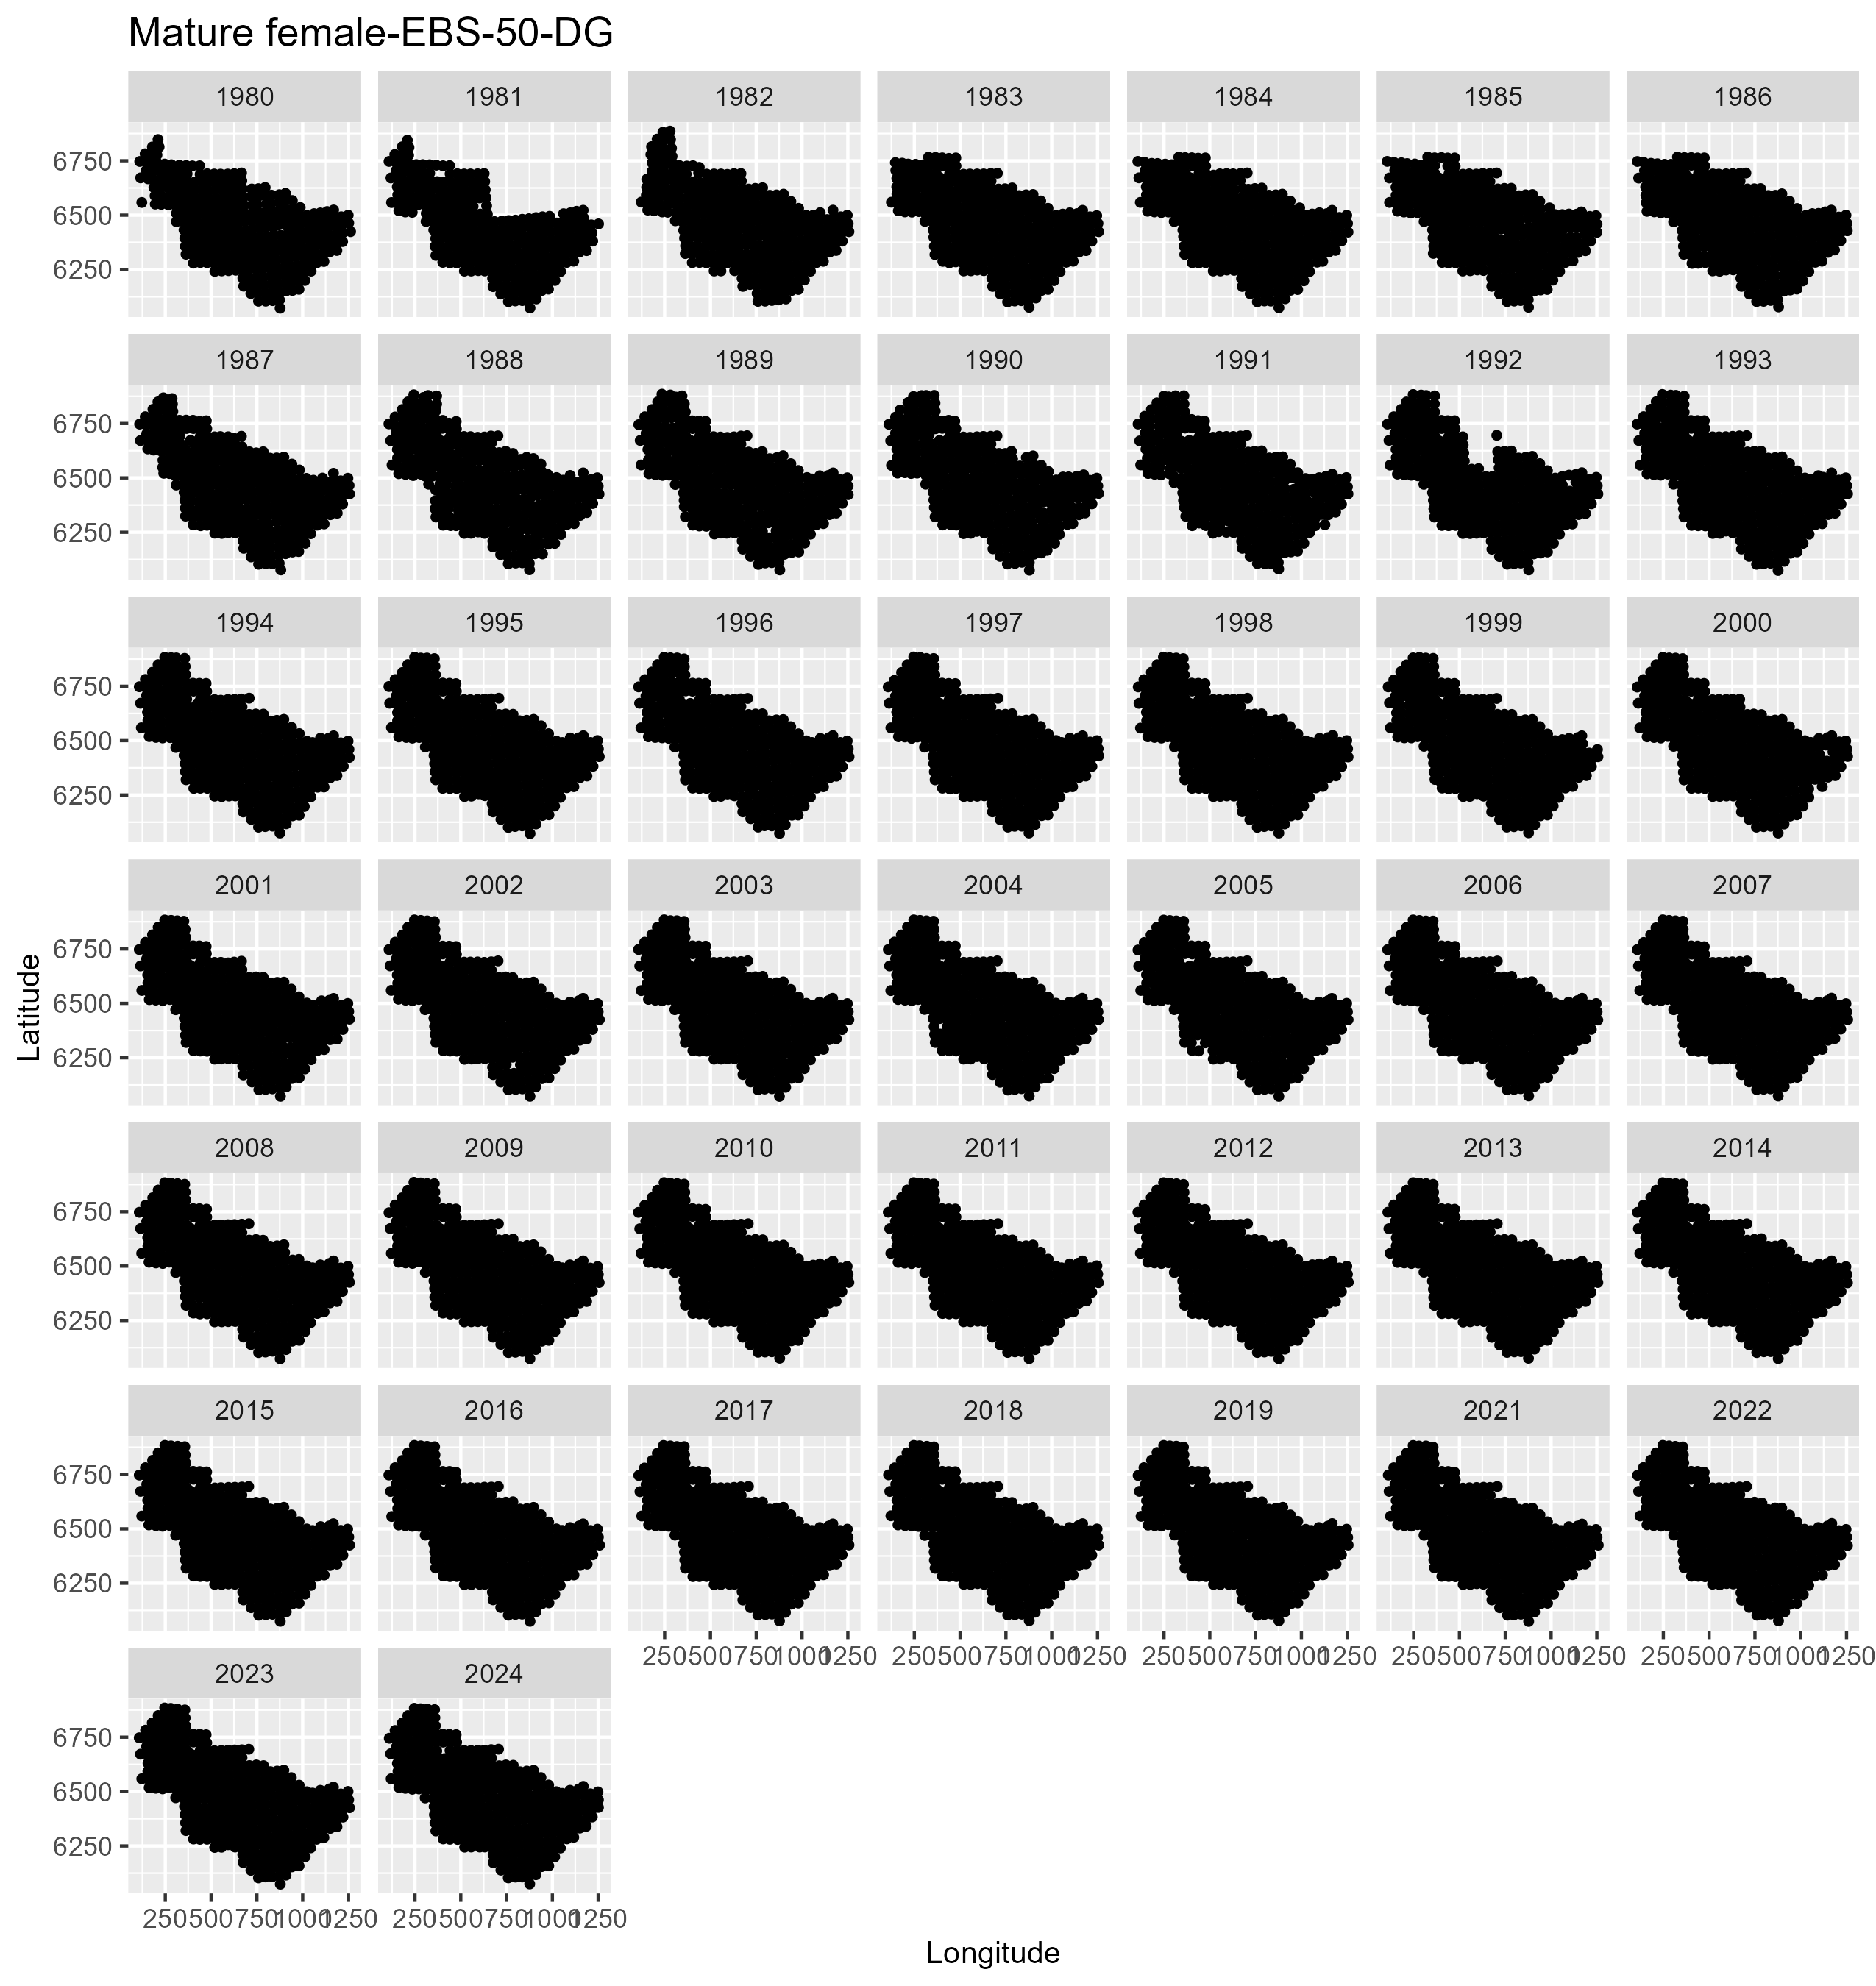
\includegraphics[width=1\linewidth,height=1\textheight]{../SNOW/Figures/DHARMa_Mature female-EBS-50-DG_SPATIAL} 

}

\caption{Spatial plot of DHARMa residuals for mature female snow crab biomass models fit using NMFS summer bottom trawl survey data from the EBS only with a 50-knot mesh and a delta-gamma model family.}\label{fig:snow-DHARMa-spat-50-matfem-EBS}
\end{figure}

\begin{figure}

{\centering 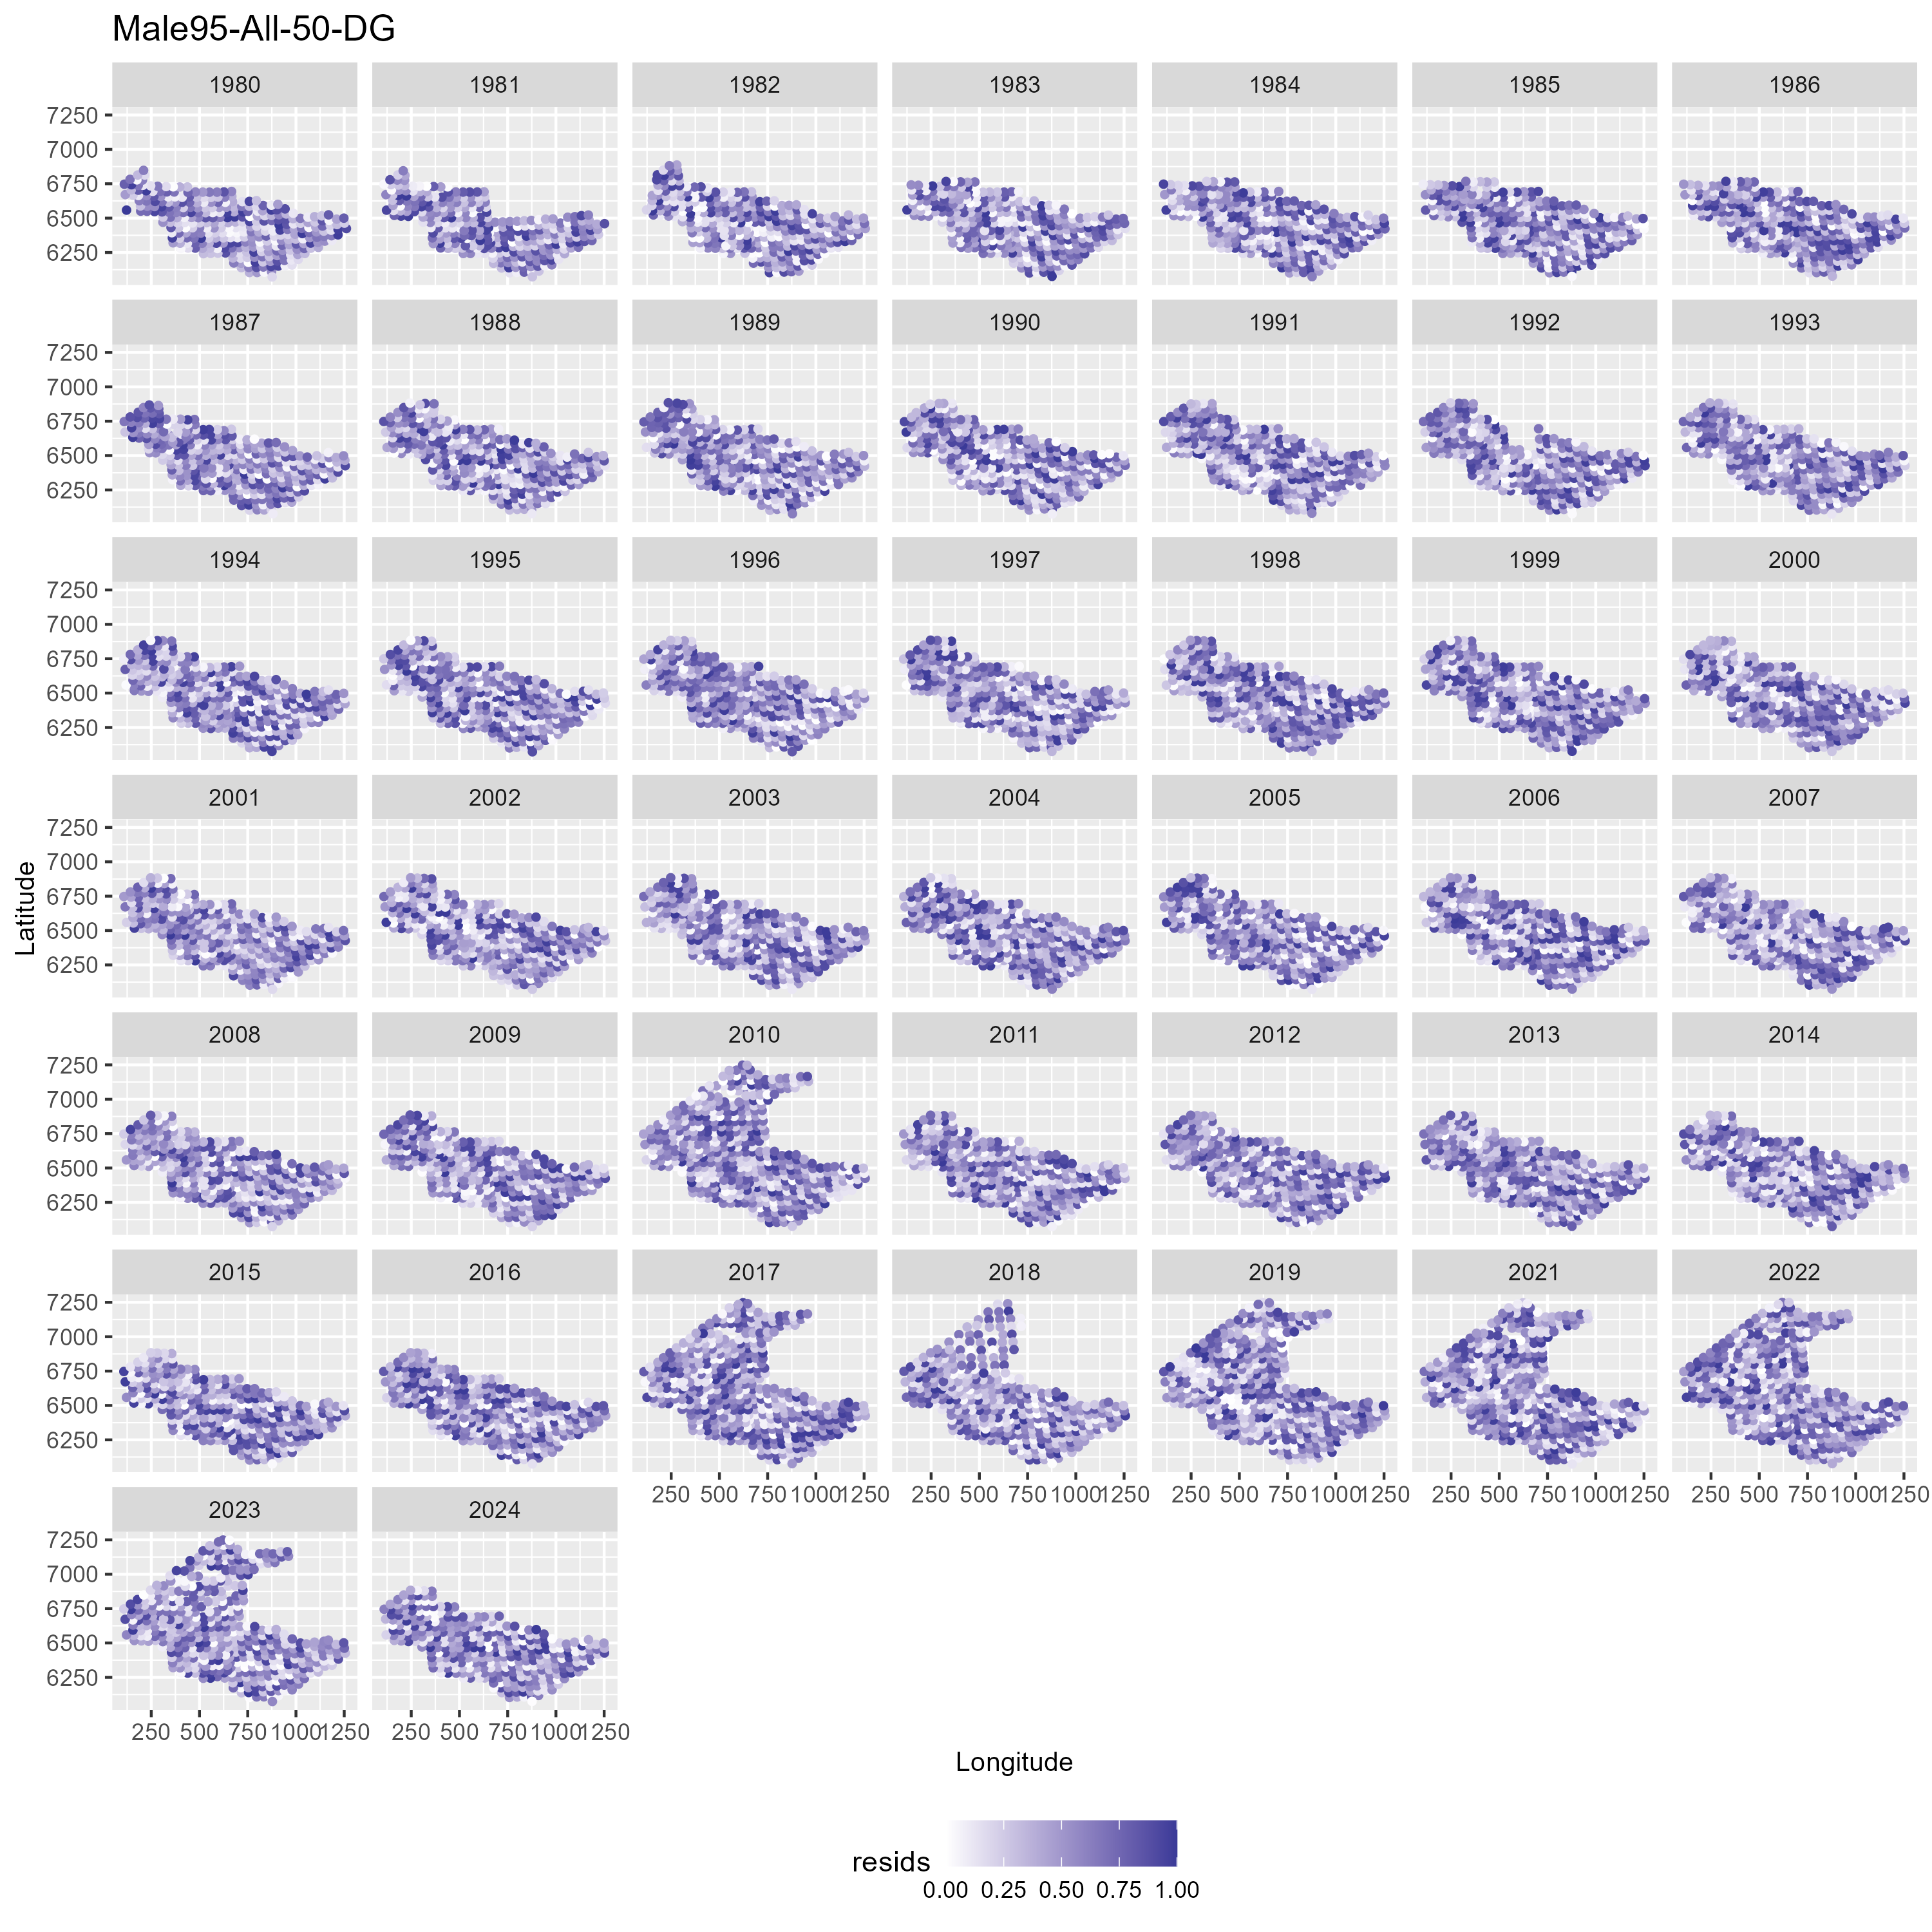
\includegraphics[width=1\linewidth,height=1\textheight]{../SNOW/Figures/DHARMa_Male95-All-50-DG_SPATIAL} 

}

\caption{Spatial plot of DHARMa residuals for male (> 95mm) snow crab biomass models fit using NMFS summer bottom trawl survey data from the EBS and NBS with a 90-knot mesh and a delta-gamma model family.}\label{fig:snow-DHARMa-spat-90-male95-EBSNBS}
\end{figure}

\begin{figure}

{\centering 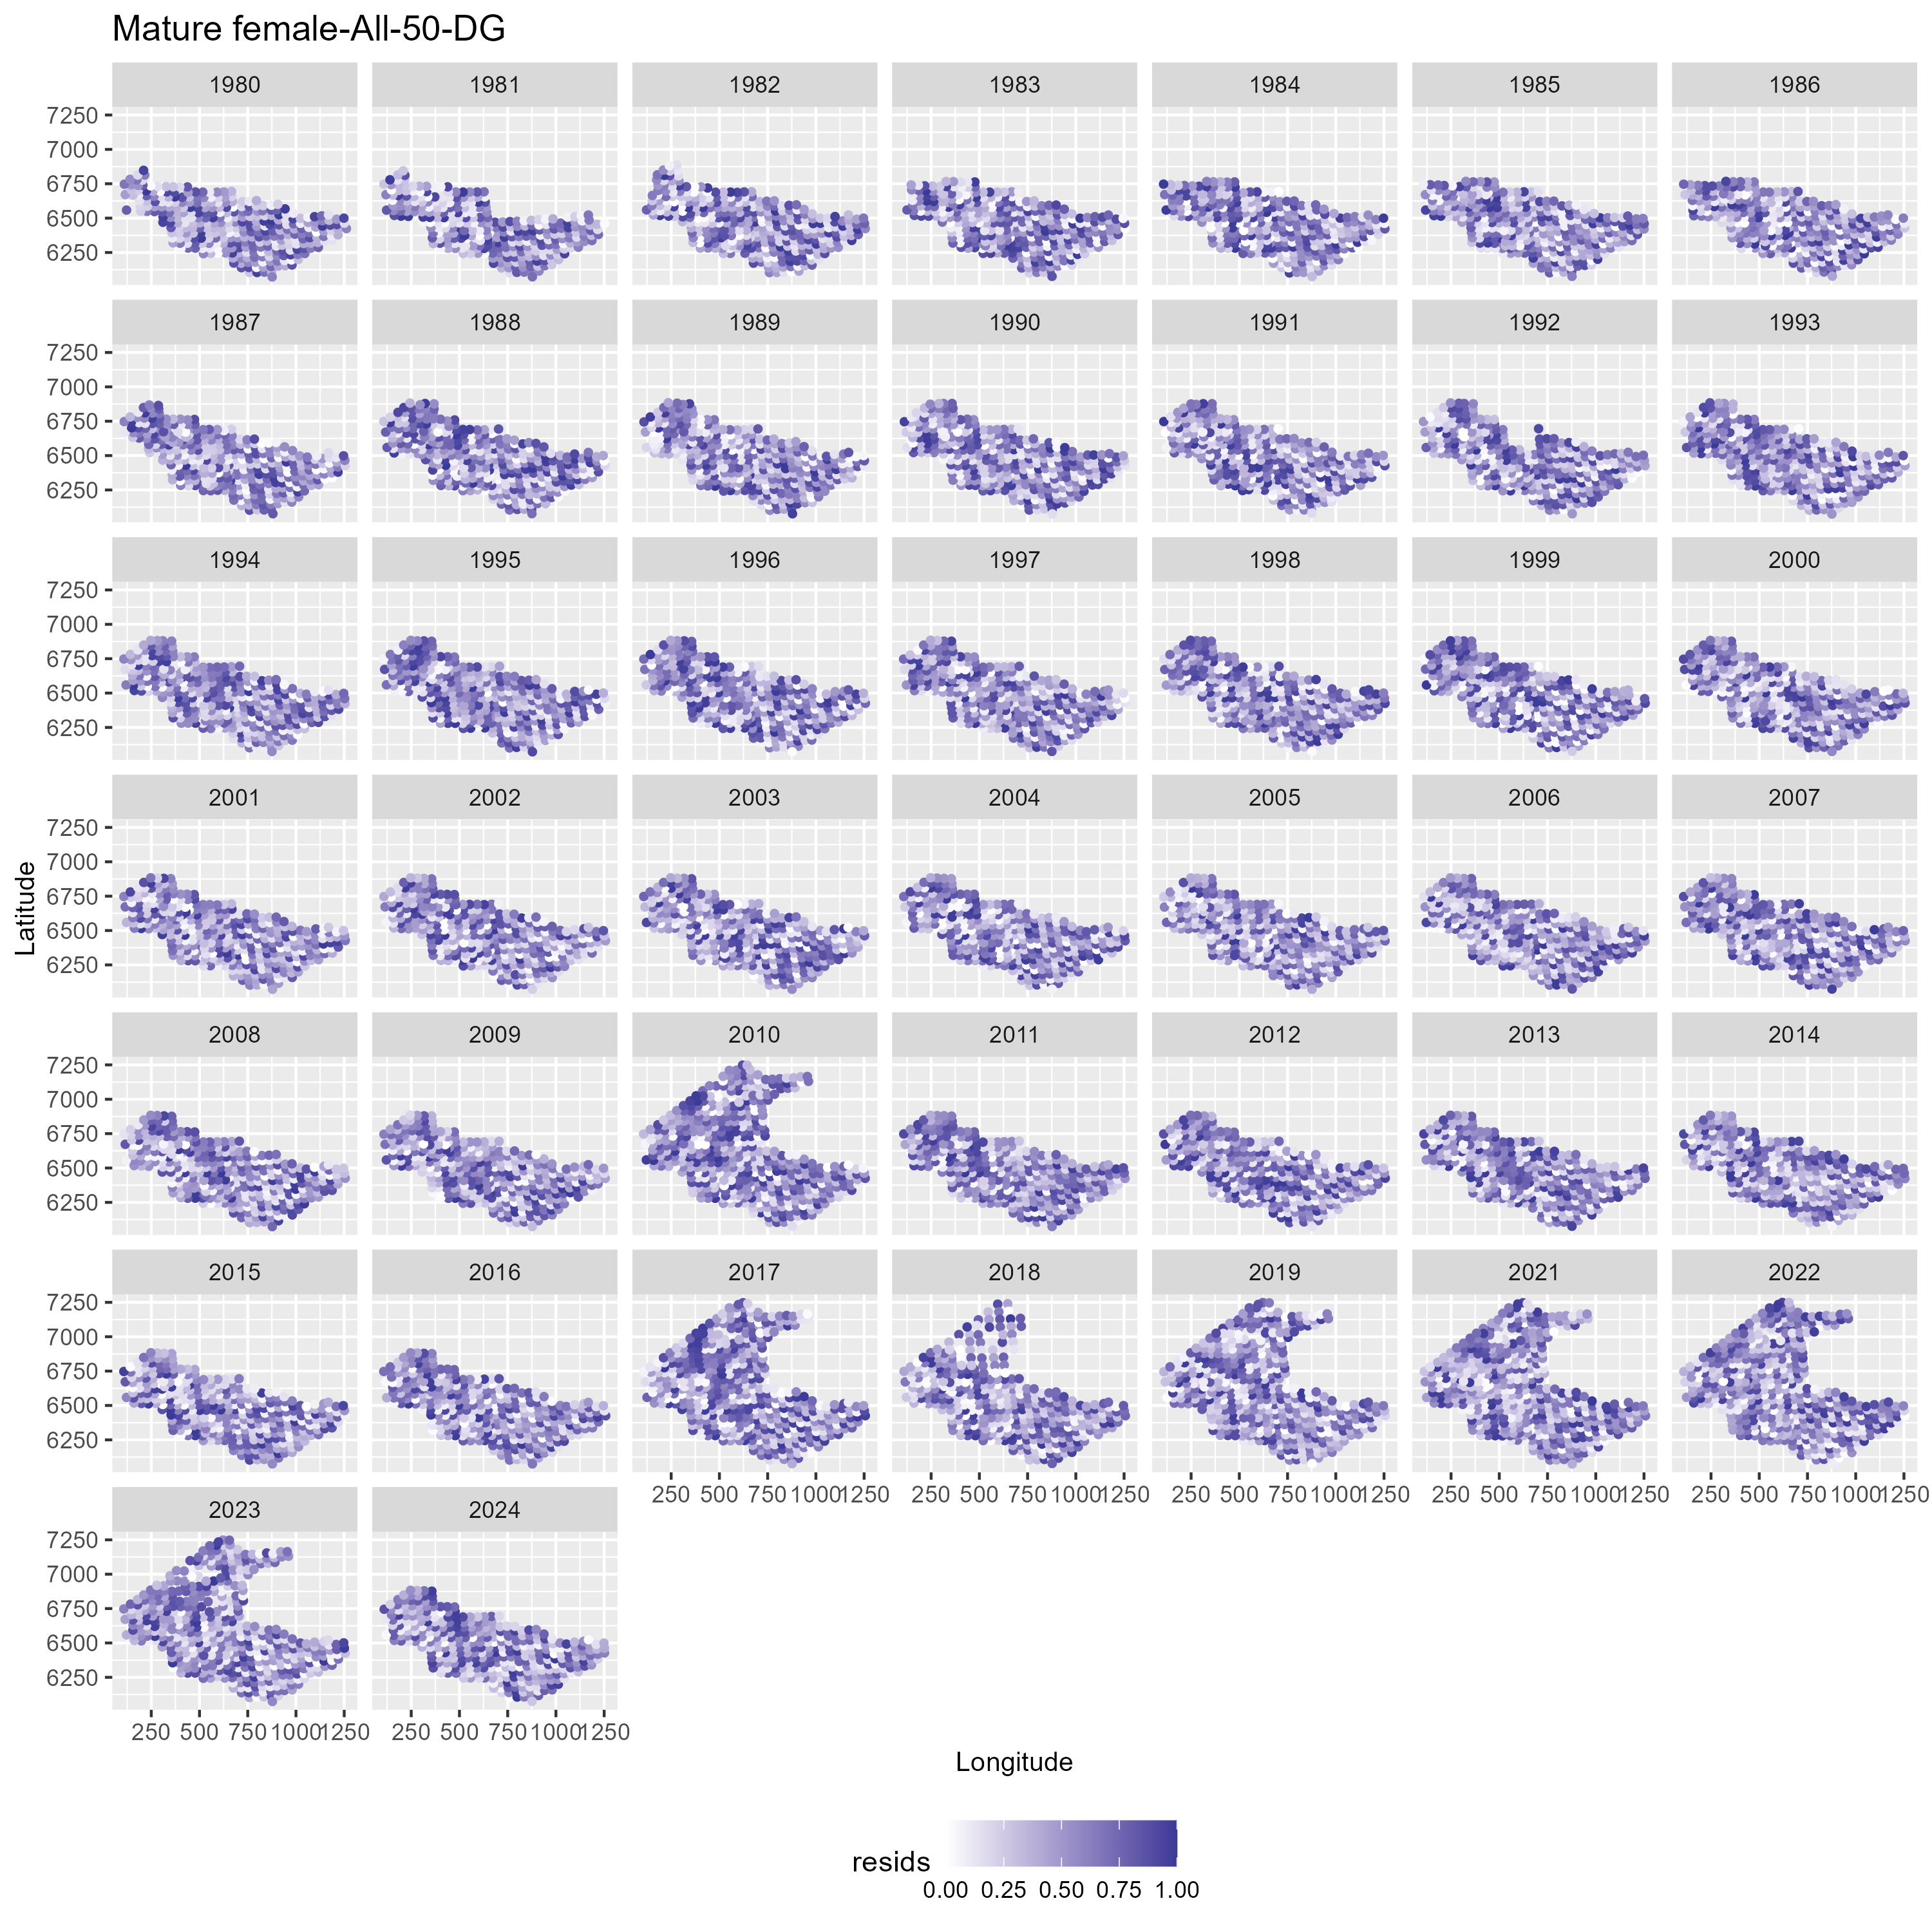
\includegraphics[width=1\linewidth,height=1\textheight]{../SNOW/Figures/DHARMa_Mature female-All-50-DG_SPATIAL} 

}

\caption{Spatial plot of DHARMa residuals for mature female snow crab biomass models fit using NMFS summer bottom trawl survey data from the EBS and NBS with a 50-knot mesh and a delta-gamma model family.}\label{fig:snow-DHARMa-spat-50-matfem-EBSNBS}
\end{figure}

\begin{figure}

{\centering 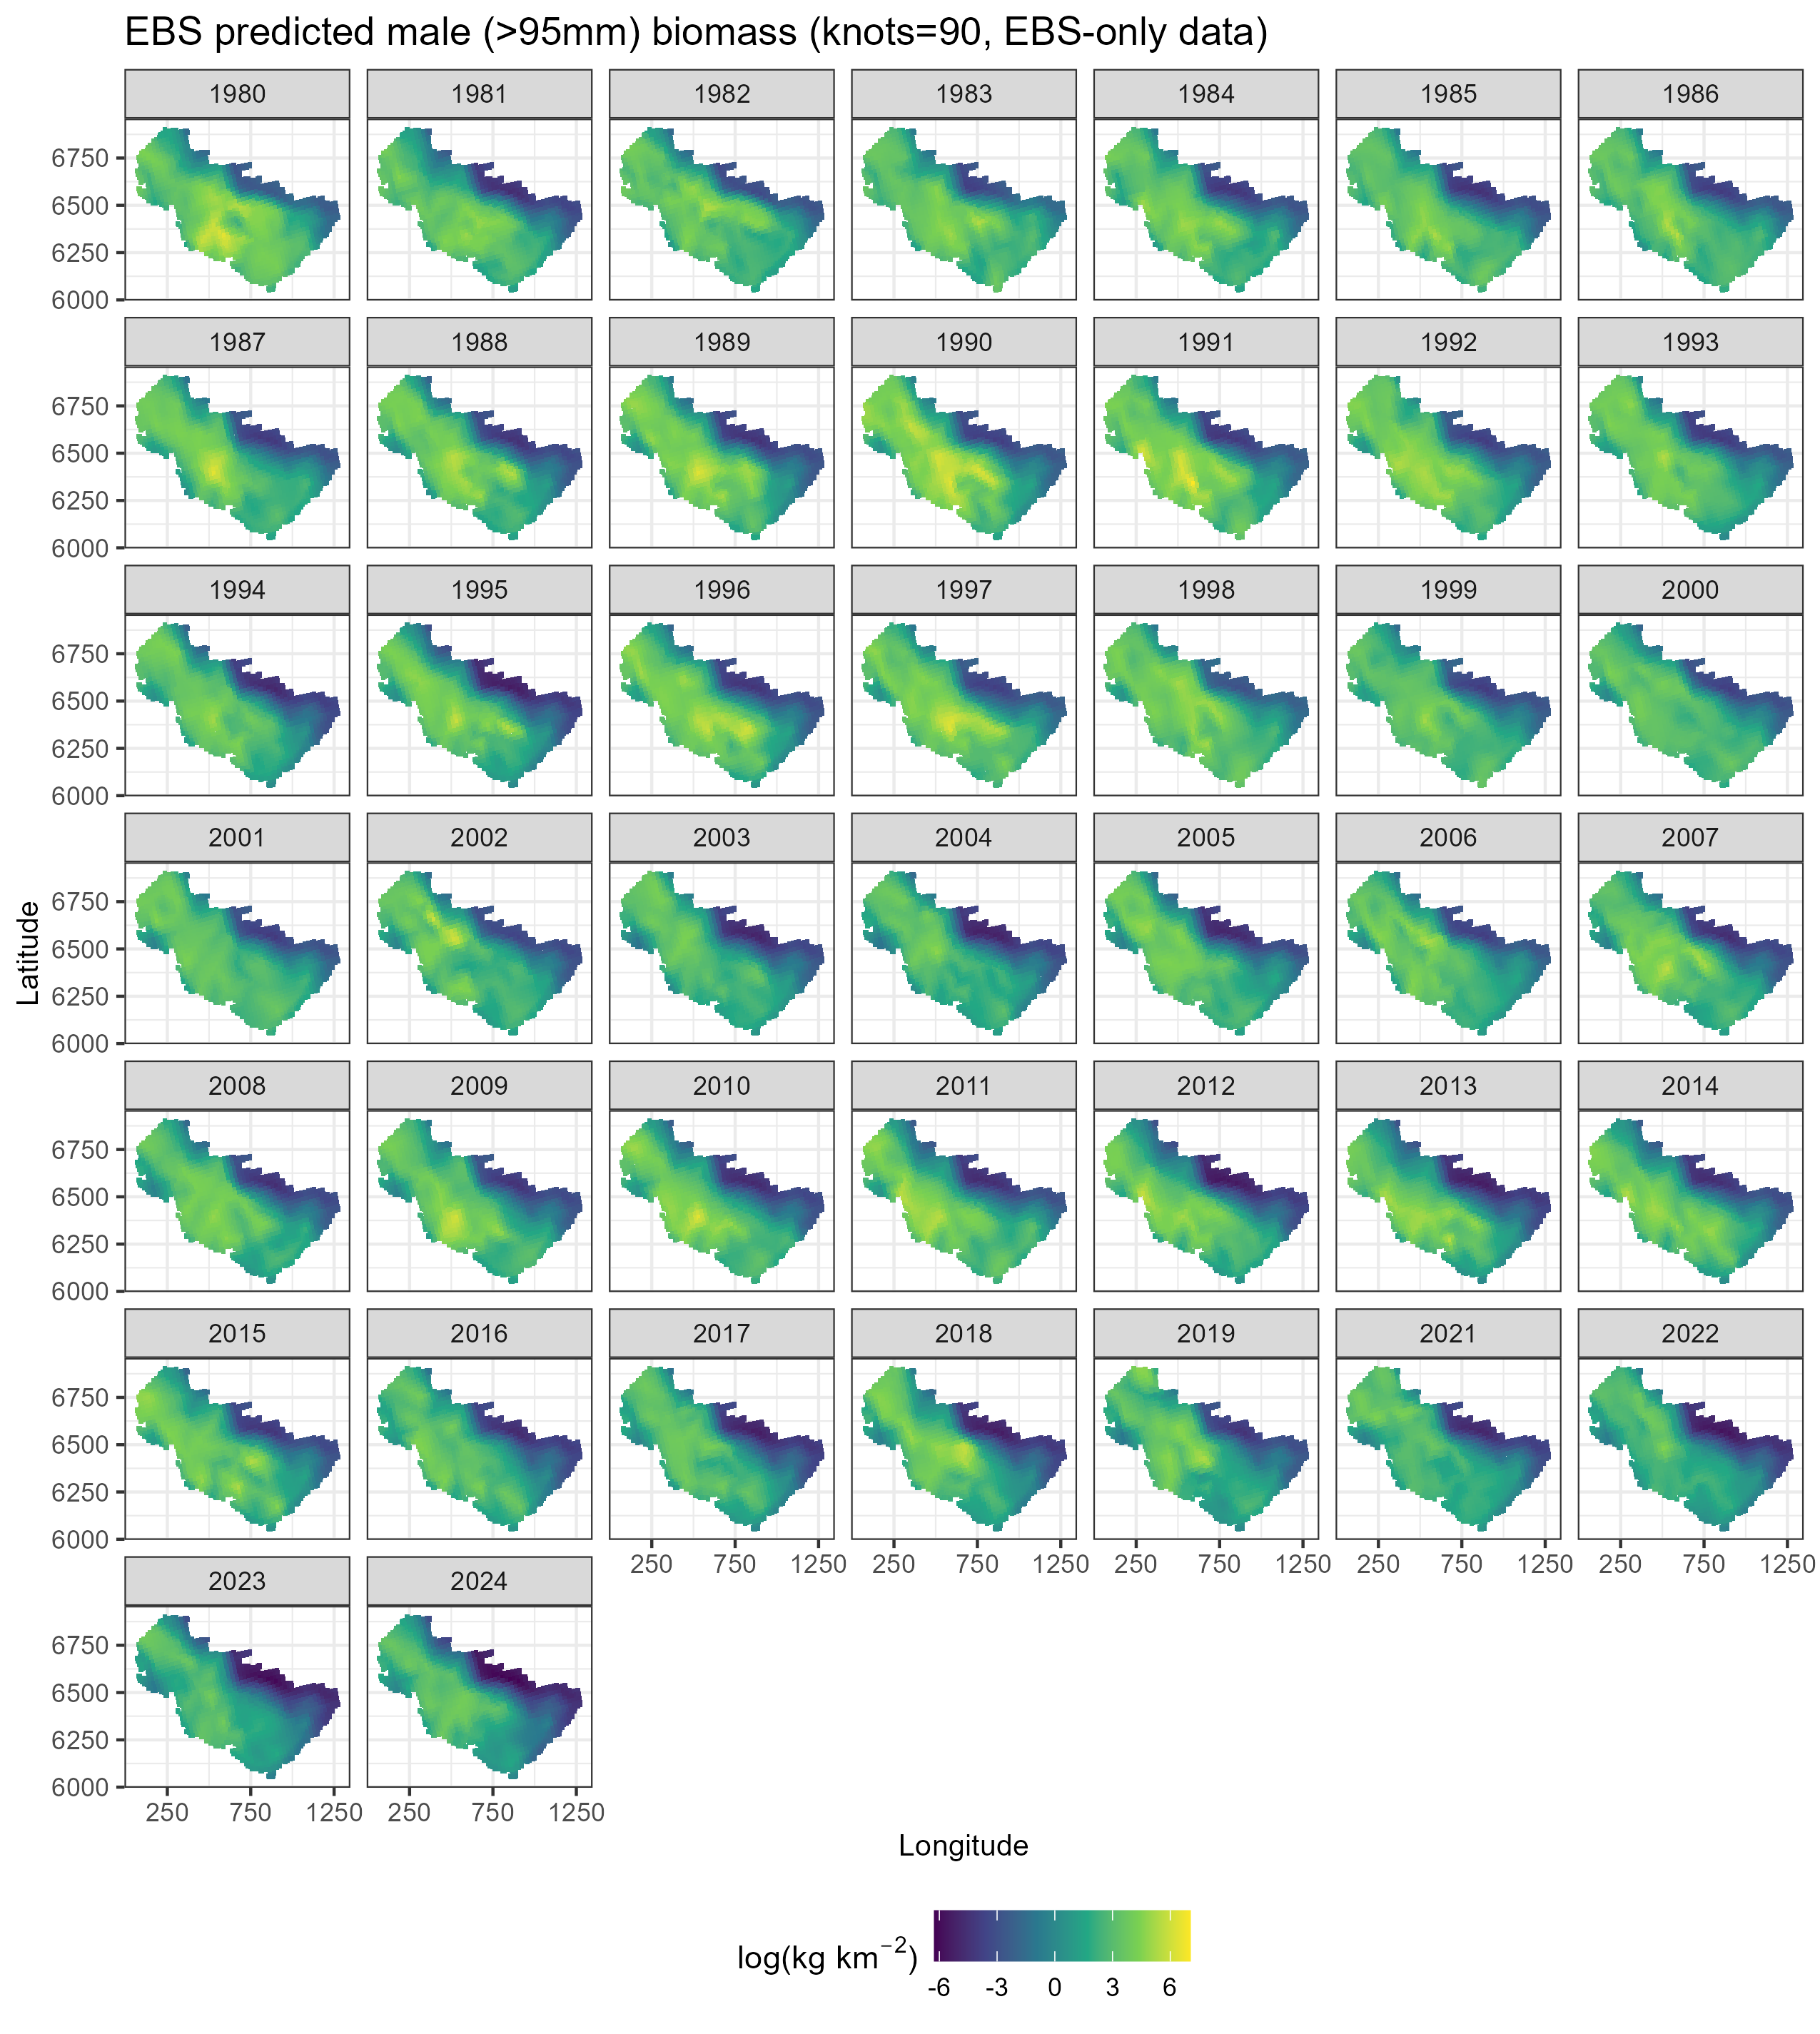
\includegraphics[width=1\linewidth,height=1\textheight]{../SNOW/Figures/EBS-90-DG-Male95_spatbio} 

}

\caption{Spatial predictions of snow crab male (>95mm) biomass across the eastern Bering Sea using NMFS summer bottom trawl survey data from the EBS only with a 90-knot mesh and a delta-gamma model family. .}\label{fig:snow-spatpred-bio-90-male-EBS}
\end{figure}

\begin{figure}

{\centering 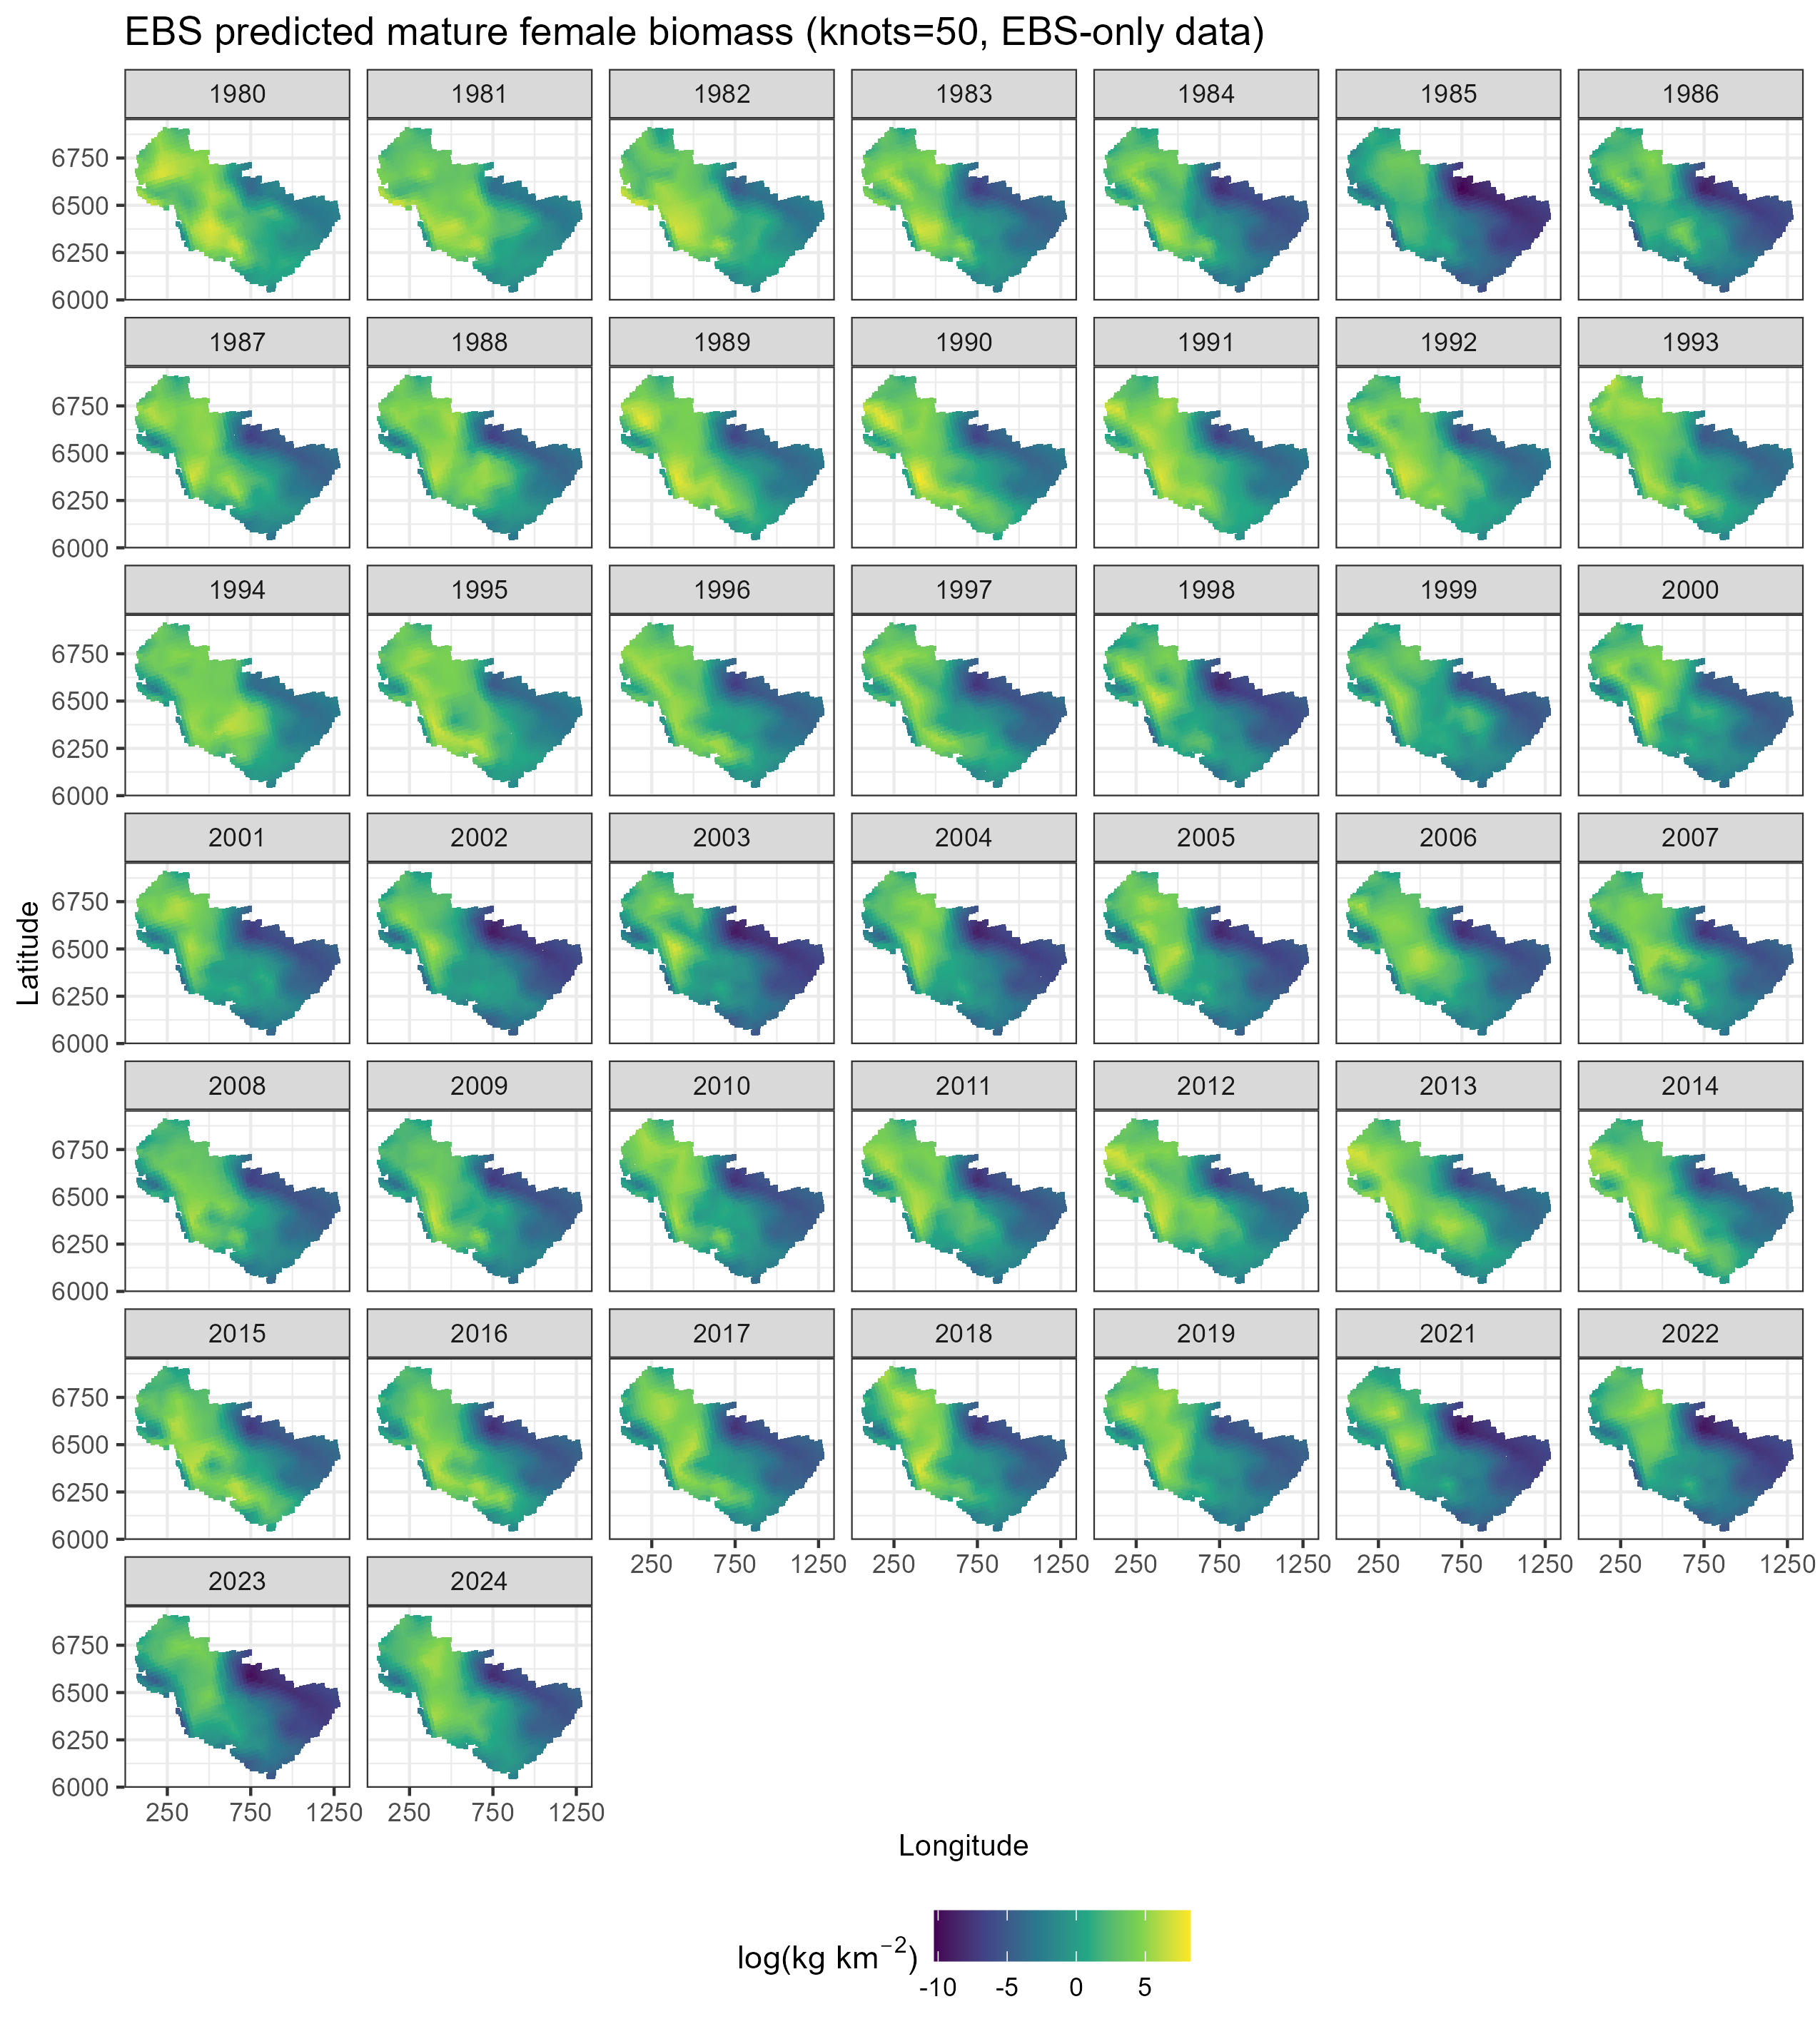
\includegraphics[width=1\linewidth,height=1\textheight]{../SNOW/Figures/EBS-50-DG-matfem_spatbio} 

}

\caption{Spatial predictions of snow crab mature female biomass across the eastern Bering Sea using NMFS summer bottom trawl survey data from the EBS only with a 50-knot mesh and a delta-gamma model family. .}\label{fig:snow-spatpred-bio-50-matfem-EBS}
\end{figure}

\begin{figure}

{\centering 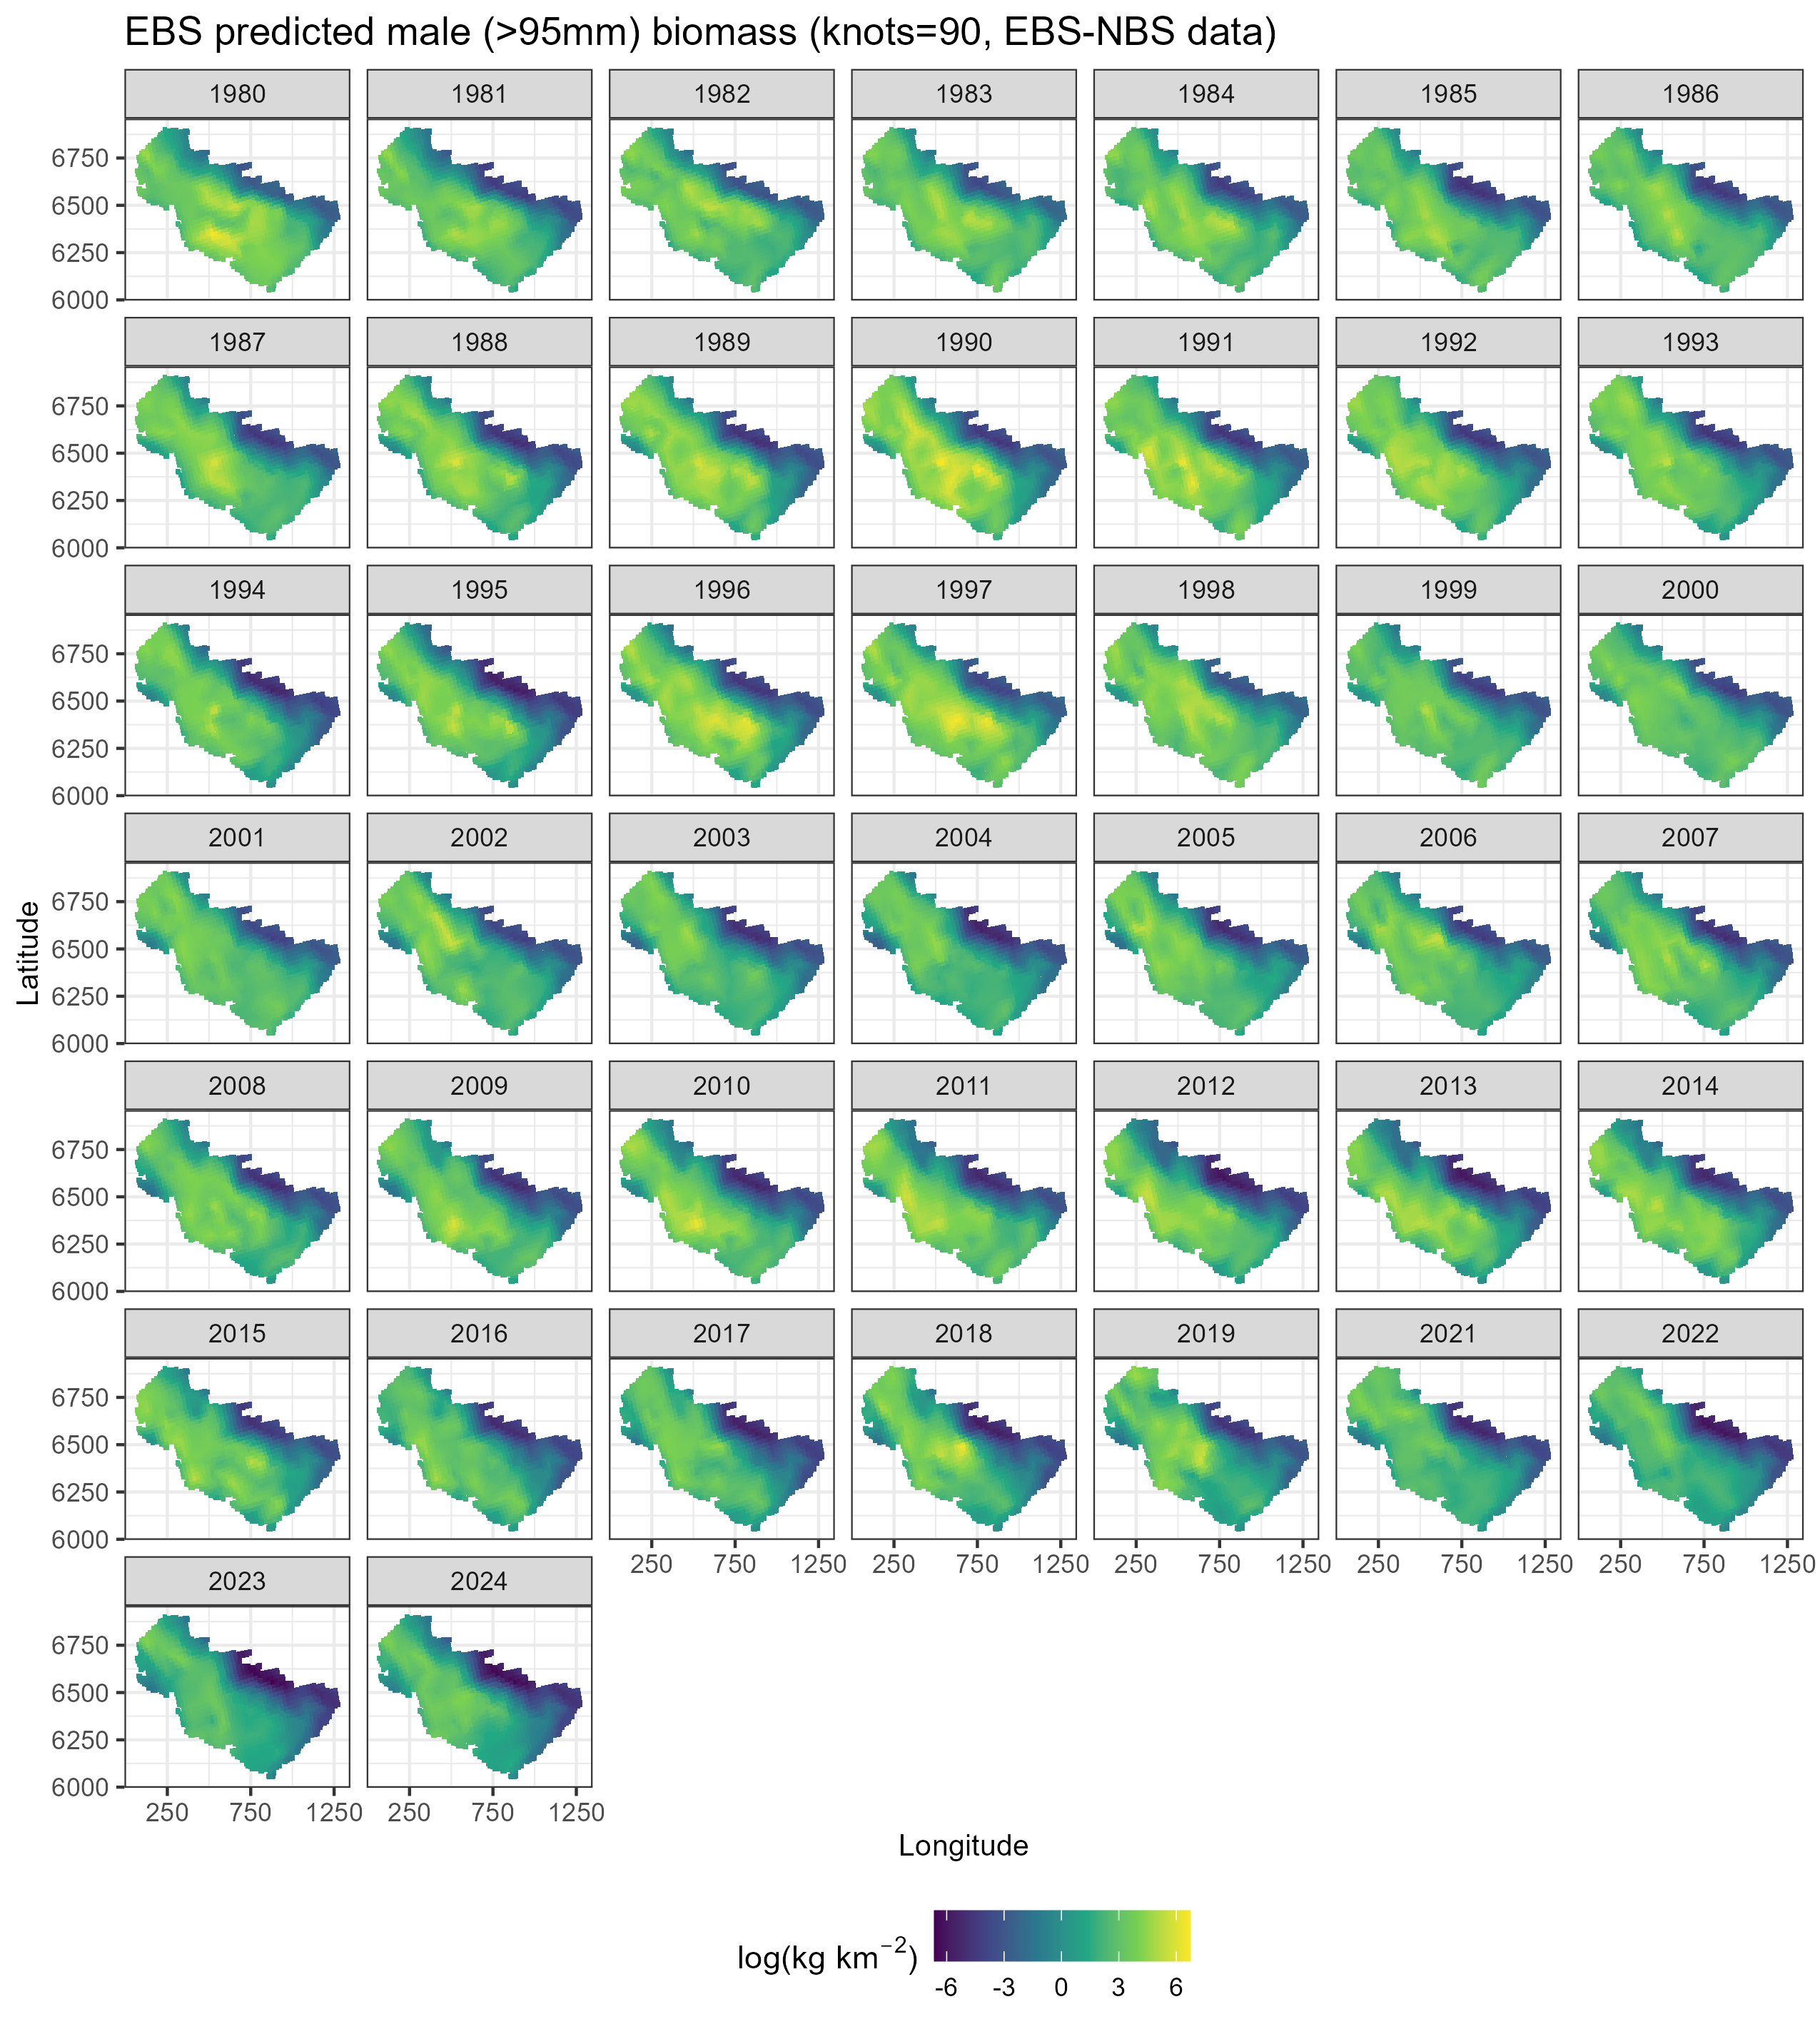
\includegraphics[width=1\linewidth,height=1\textheight]{../SNOW/Figures/EBSNBS-90-DG-Male95_spatbio} 

}

\caption{Spatial predictions of snow crab male (>95mm) biomass across the eastern Bering Sea using NMFS summer bottom trawl survey data from the EBS and NBS with a 90-knot mesh and a delta-gamma model family. .}\label{fig:snow-spatpred-bio-90-male-EBSNBS}
\end{figure}

\begin{figure}

{\centering 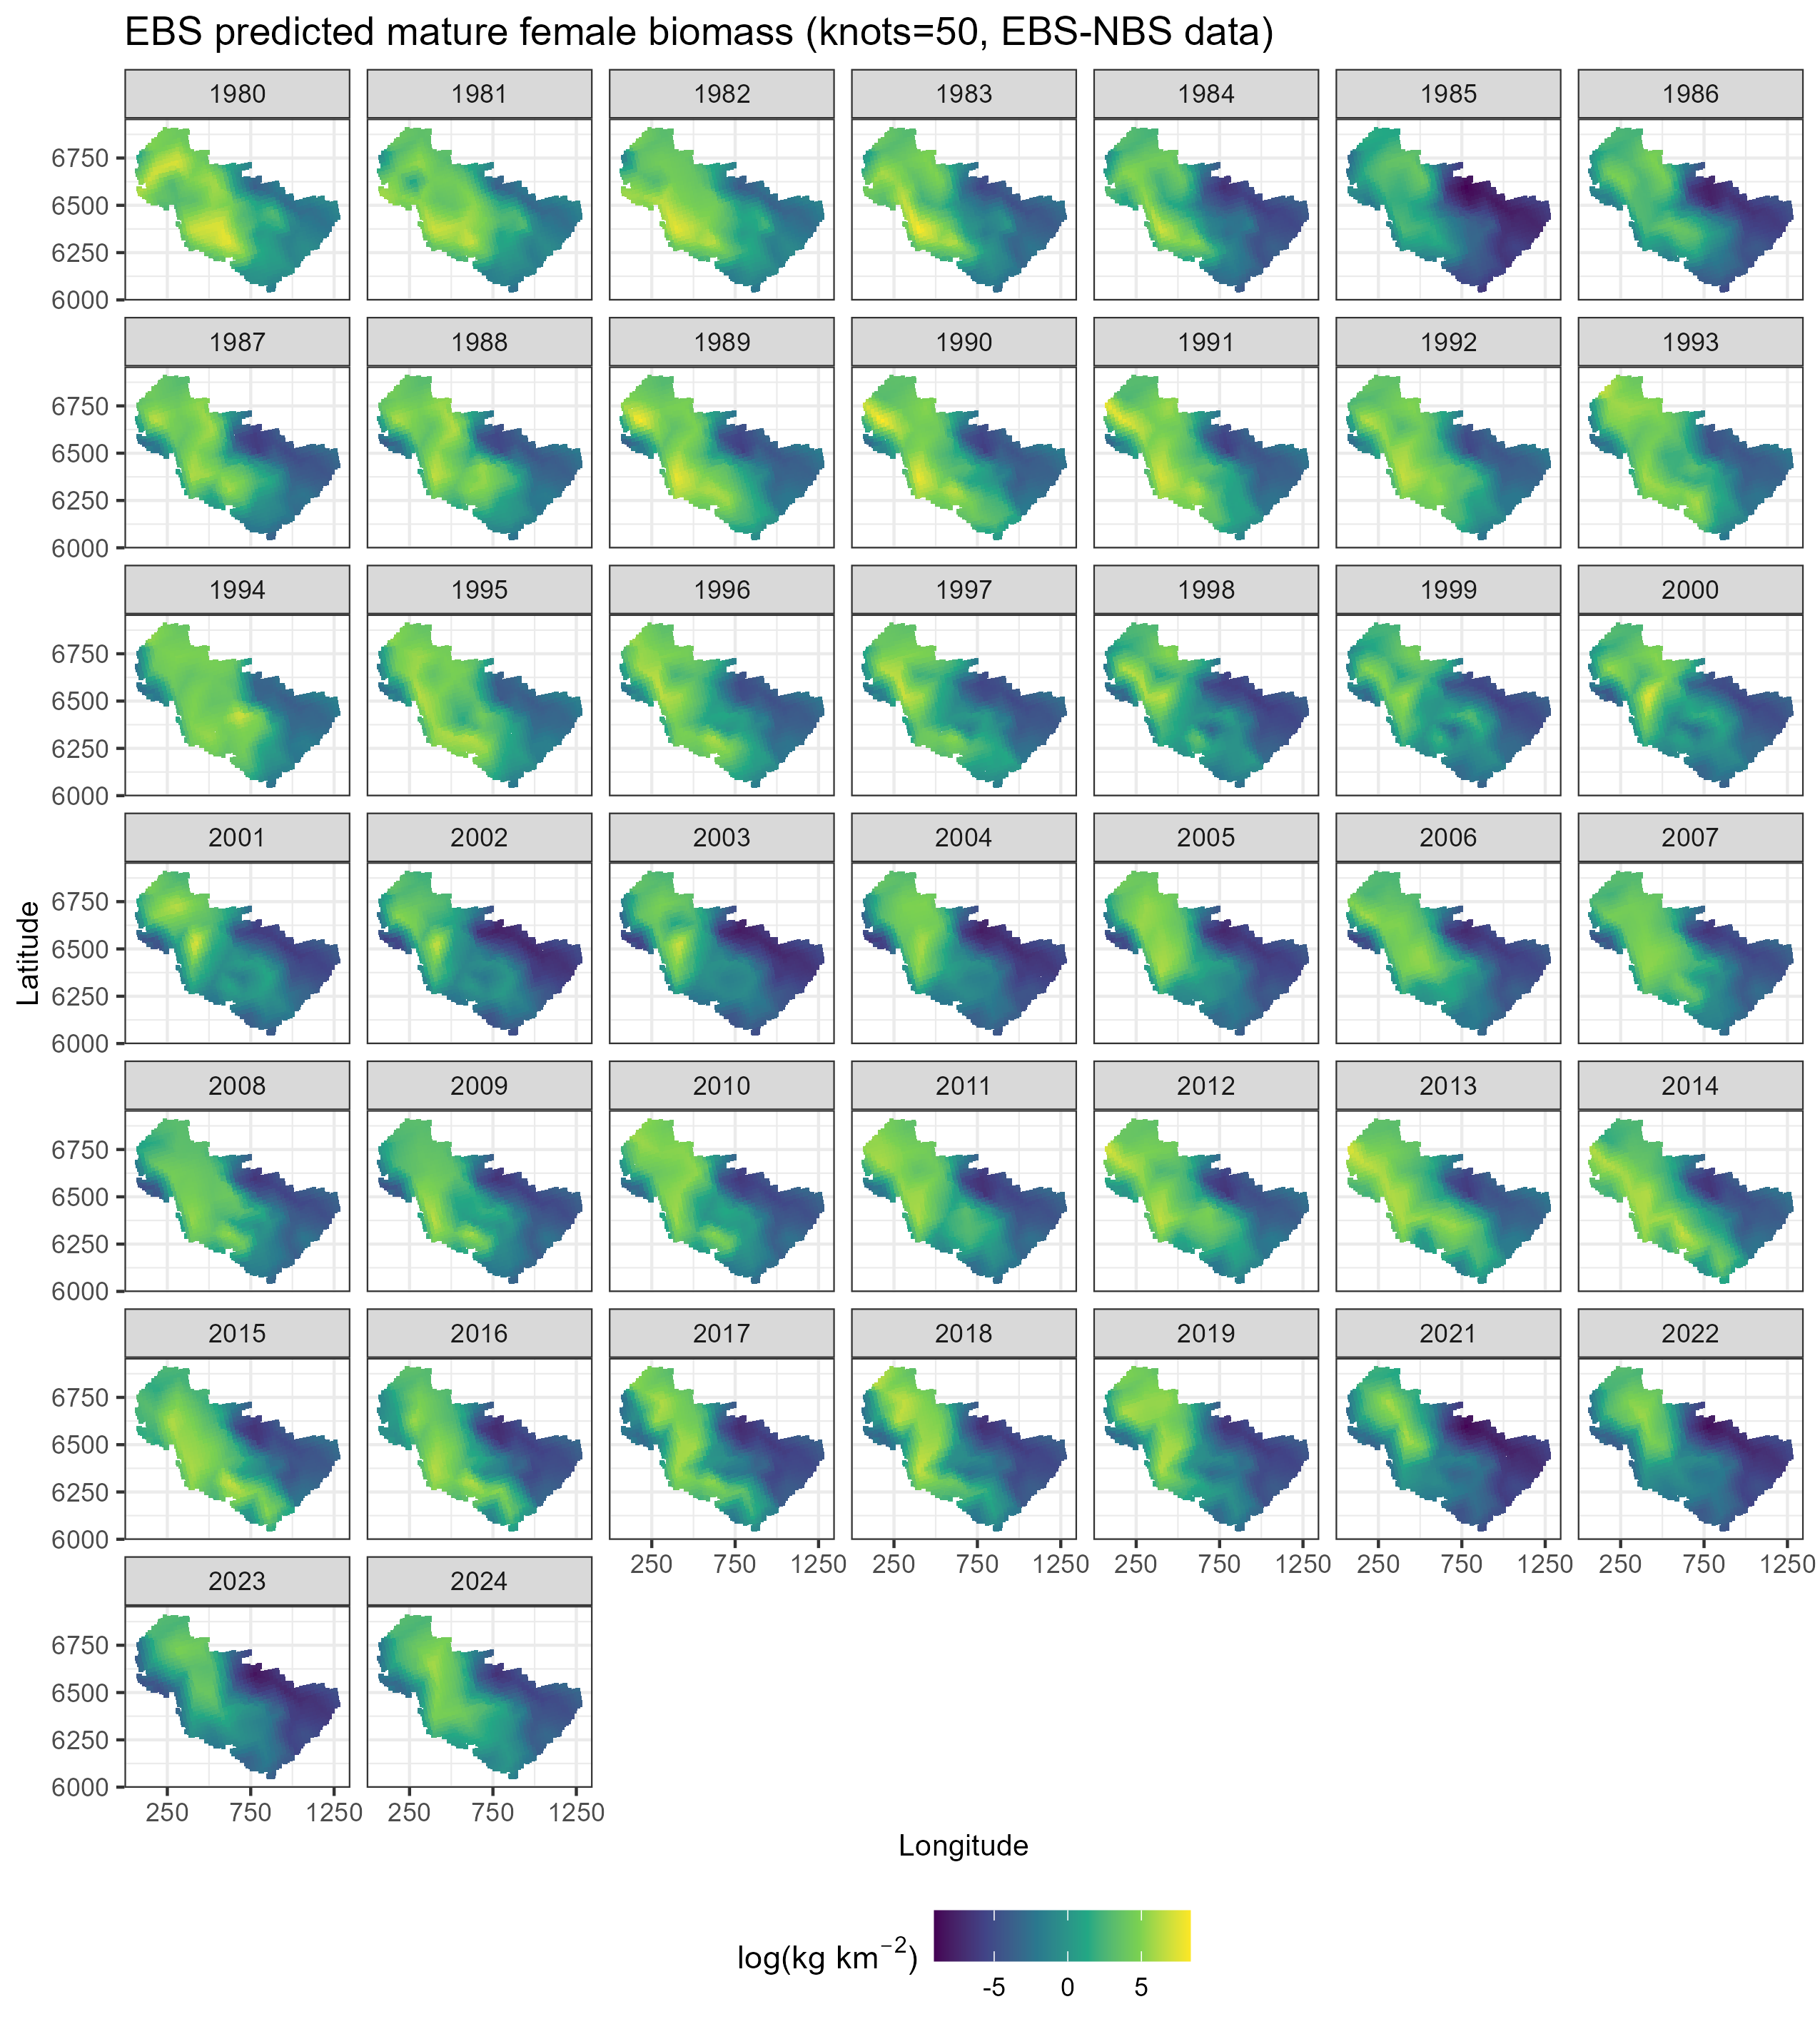
\includegraphics[width=1\linewidth,height=1\textheight]{../SNOW/Figures/EBSNBS-50-DG-matfem_spatbio} 

}

\caption{Spatial predictions of snow crab mature female biomass across the eastern Bering Sea using NMFS summer bottom trawl survey data from the EBS and NBS with a 50-knot mesh and a delta-gamma model family. .}\label{fig:snow-spatpred-bio-50-matfem-EBSNBS}
\end{figure}

\begin{figure}

{\centering 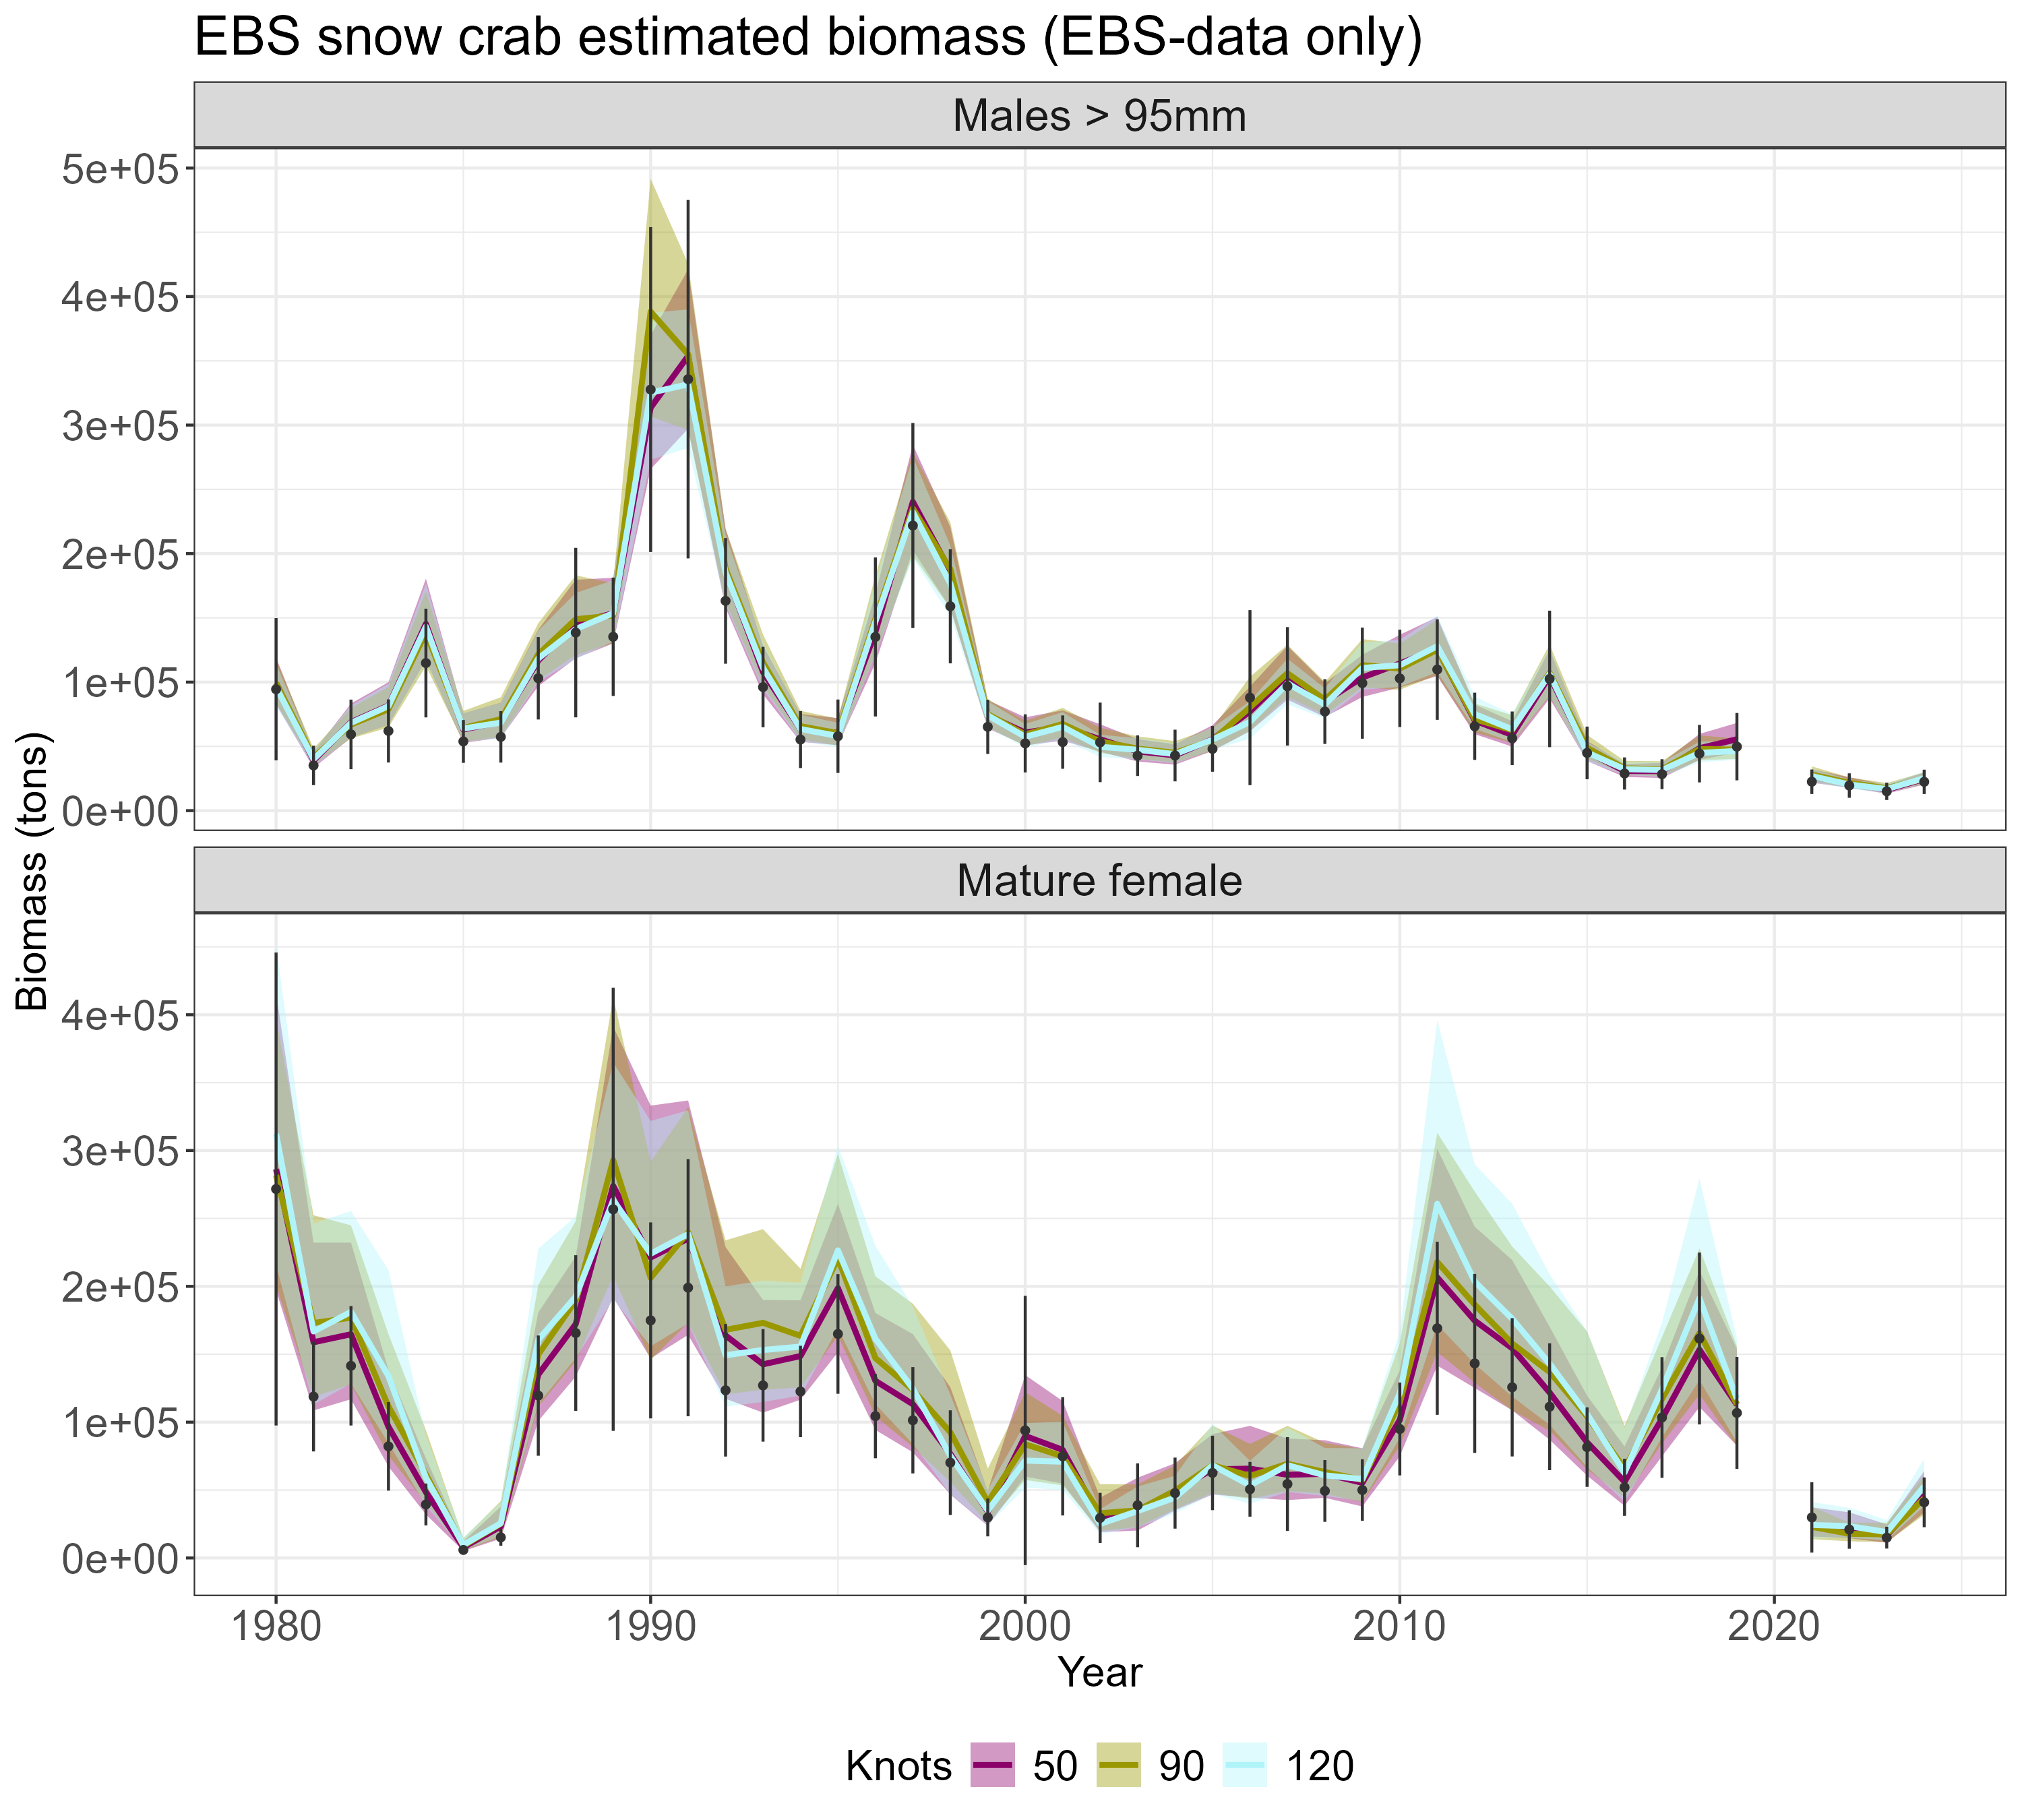
\includegraphics[width=1\linewidth,height=1\textheight]{../SNOW/Figures/snowEBS.biomass.index} 

}

\caption{Estimated biomass (tons) for eastern Bering Sea snow crab. Colored lines represent biomass (±95\% CI) estimated by sdmTMB in a delta-model framework, with orange, blue, and pink denoting models fit with a 50-, 90-, and 120-knot mesh, respectively. Black points represent biomass (±95\% CI) estimated by the NMFS summer bottom trawl survey.}\label{fig:snow-bio-index-EBS}
\end{figure}
\begin{figure}

{\centering 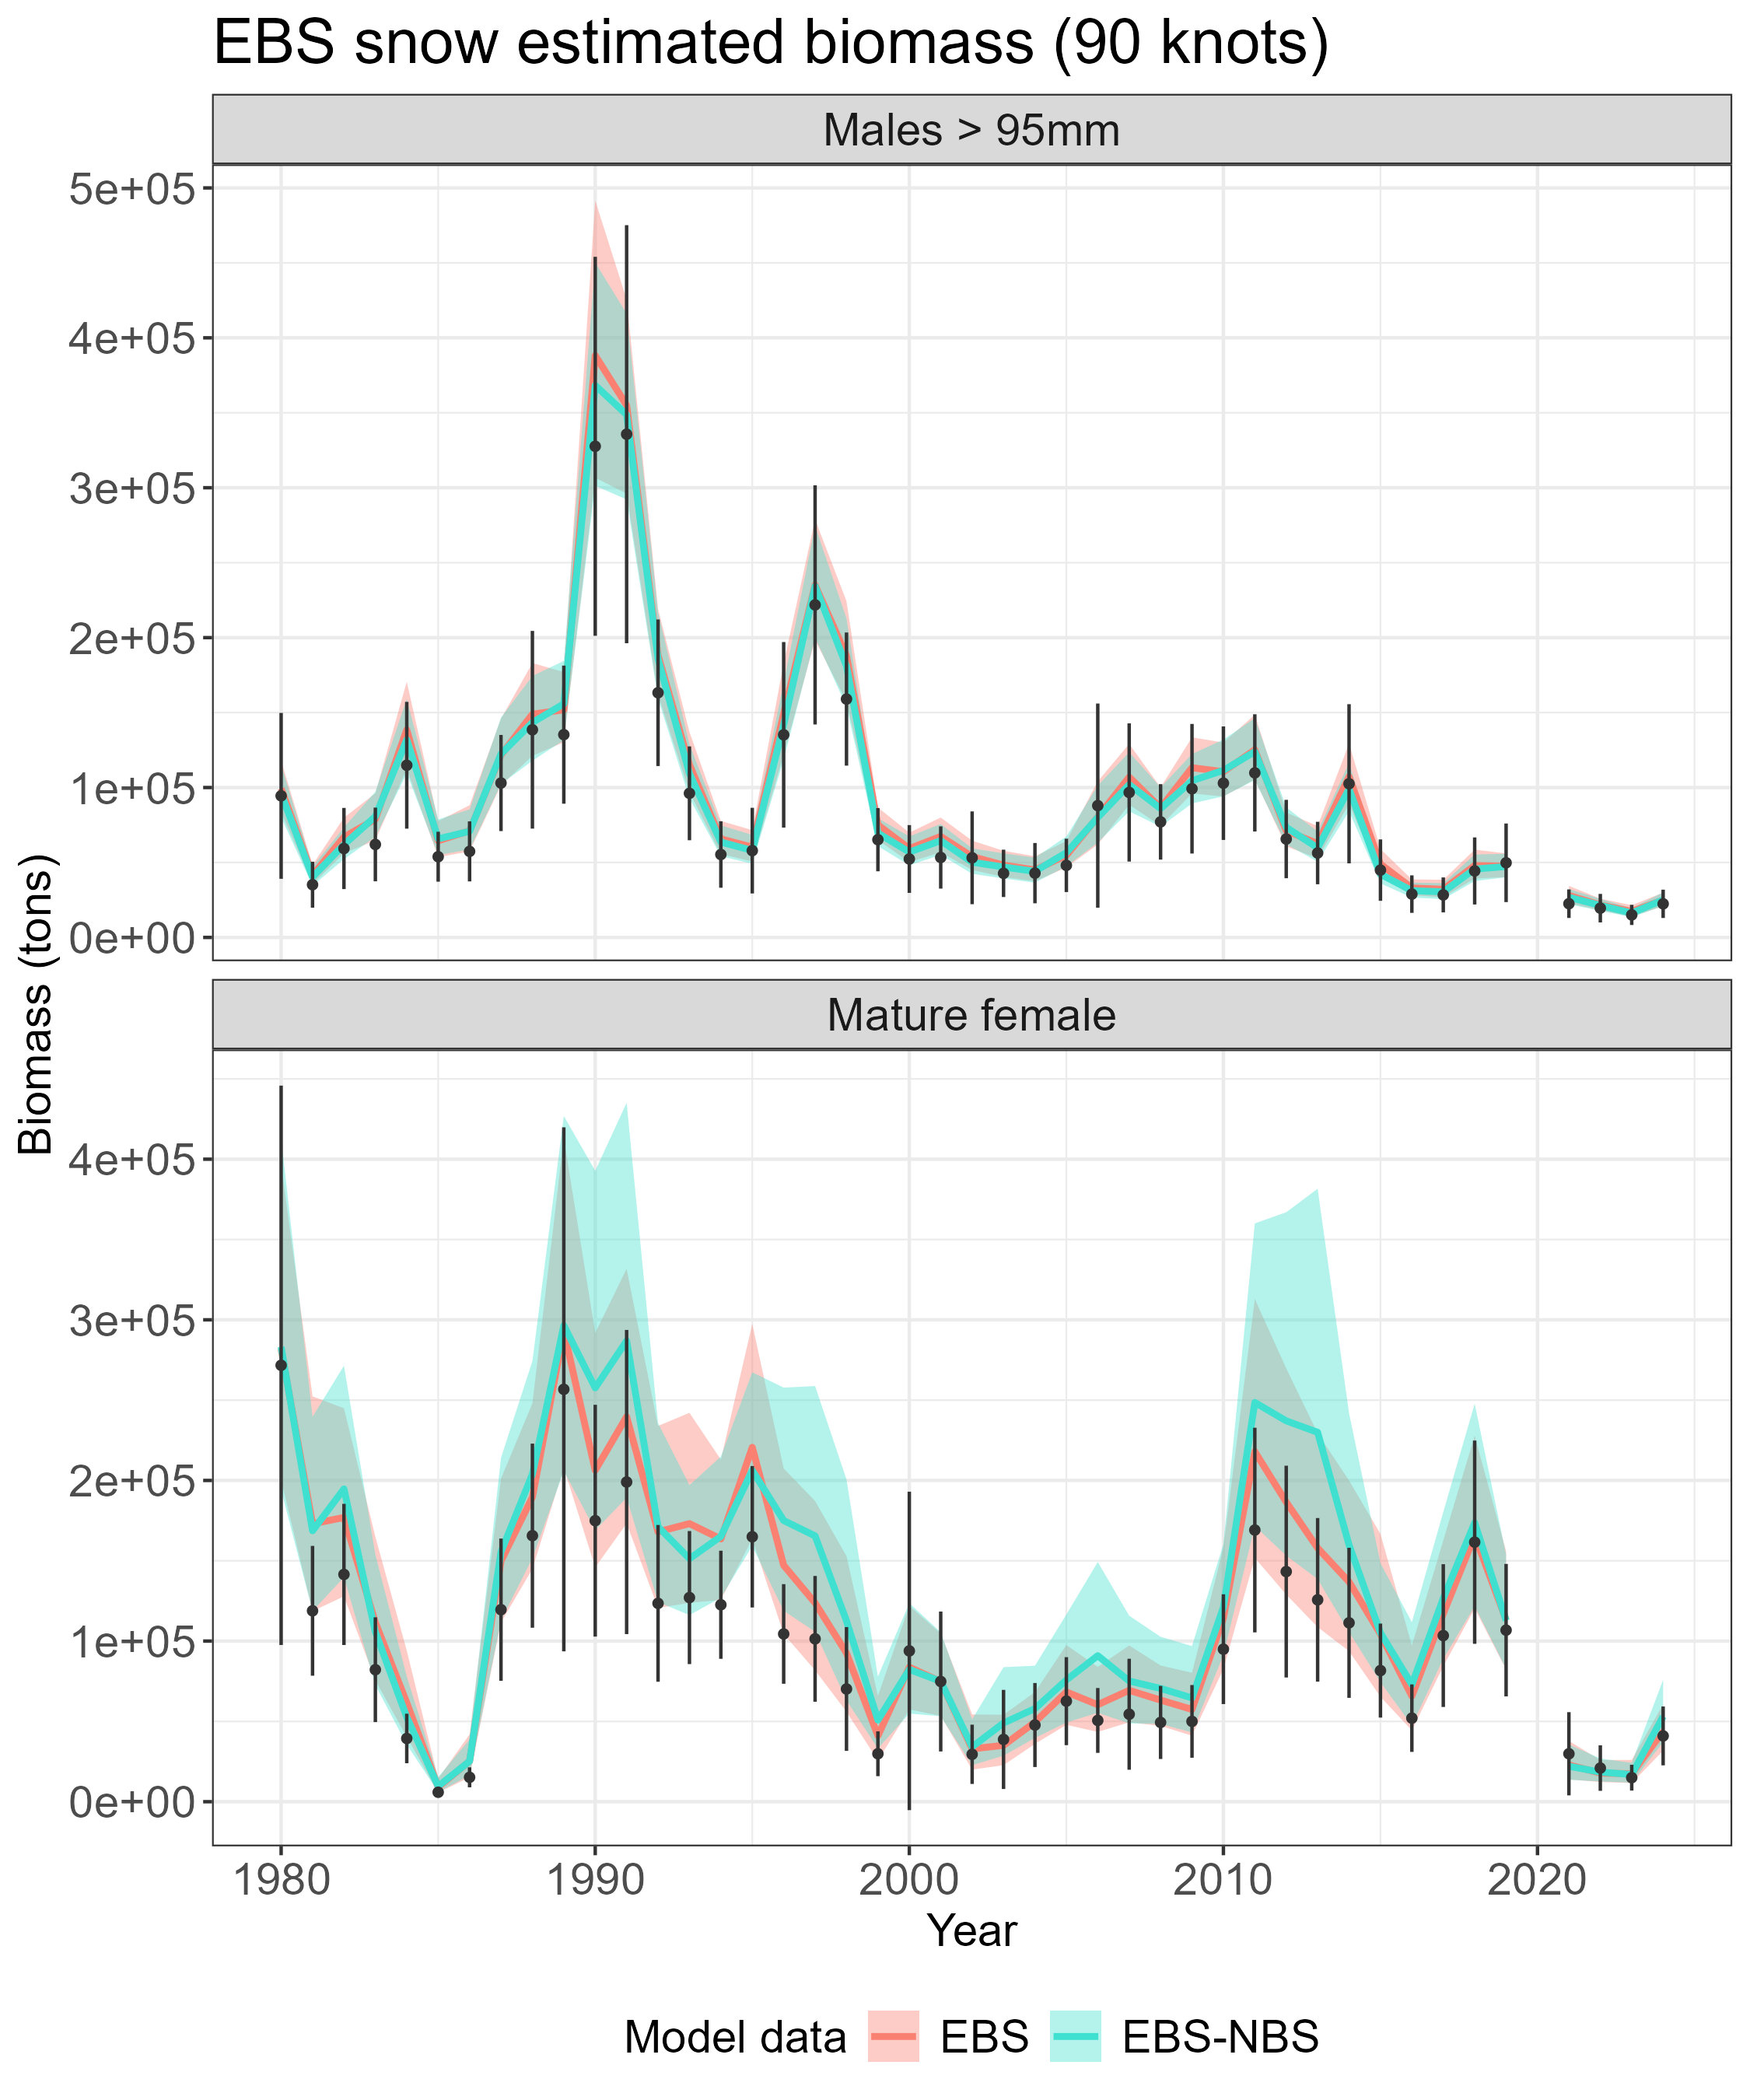
\includegraphics[width=1\linewidth,height=1\textheight]{../SNOW/Figures/snowEBSNBS.biomass.index} 

}

\caption{Estimated biomass (tons) for eastern Bering Sea snow crab. Colored lines represent biomass (±95\% CI) estimated by sdmTMB in a delta-model framework for males > 95mm using a 90-knot mesh (top) and mature females using a 50-knot mesh (bottom), with pink and blue lines denoting models fit with EBS data only and EBS-NBS data combined, respectively. Black points represent biomass (±95\% CI) estimated by the NMFS summer bottom trawl survey.}\label{fig:snow-bio-index-EBSNBS}
\end{figure}

\clearpage

\section*{Appendix}\label{appendix}
\addcontentsline{toc}{section}{Appendix}

\begin{figure}

{\centering 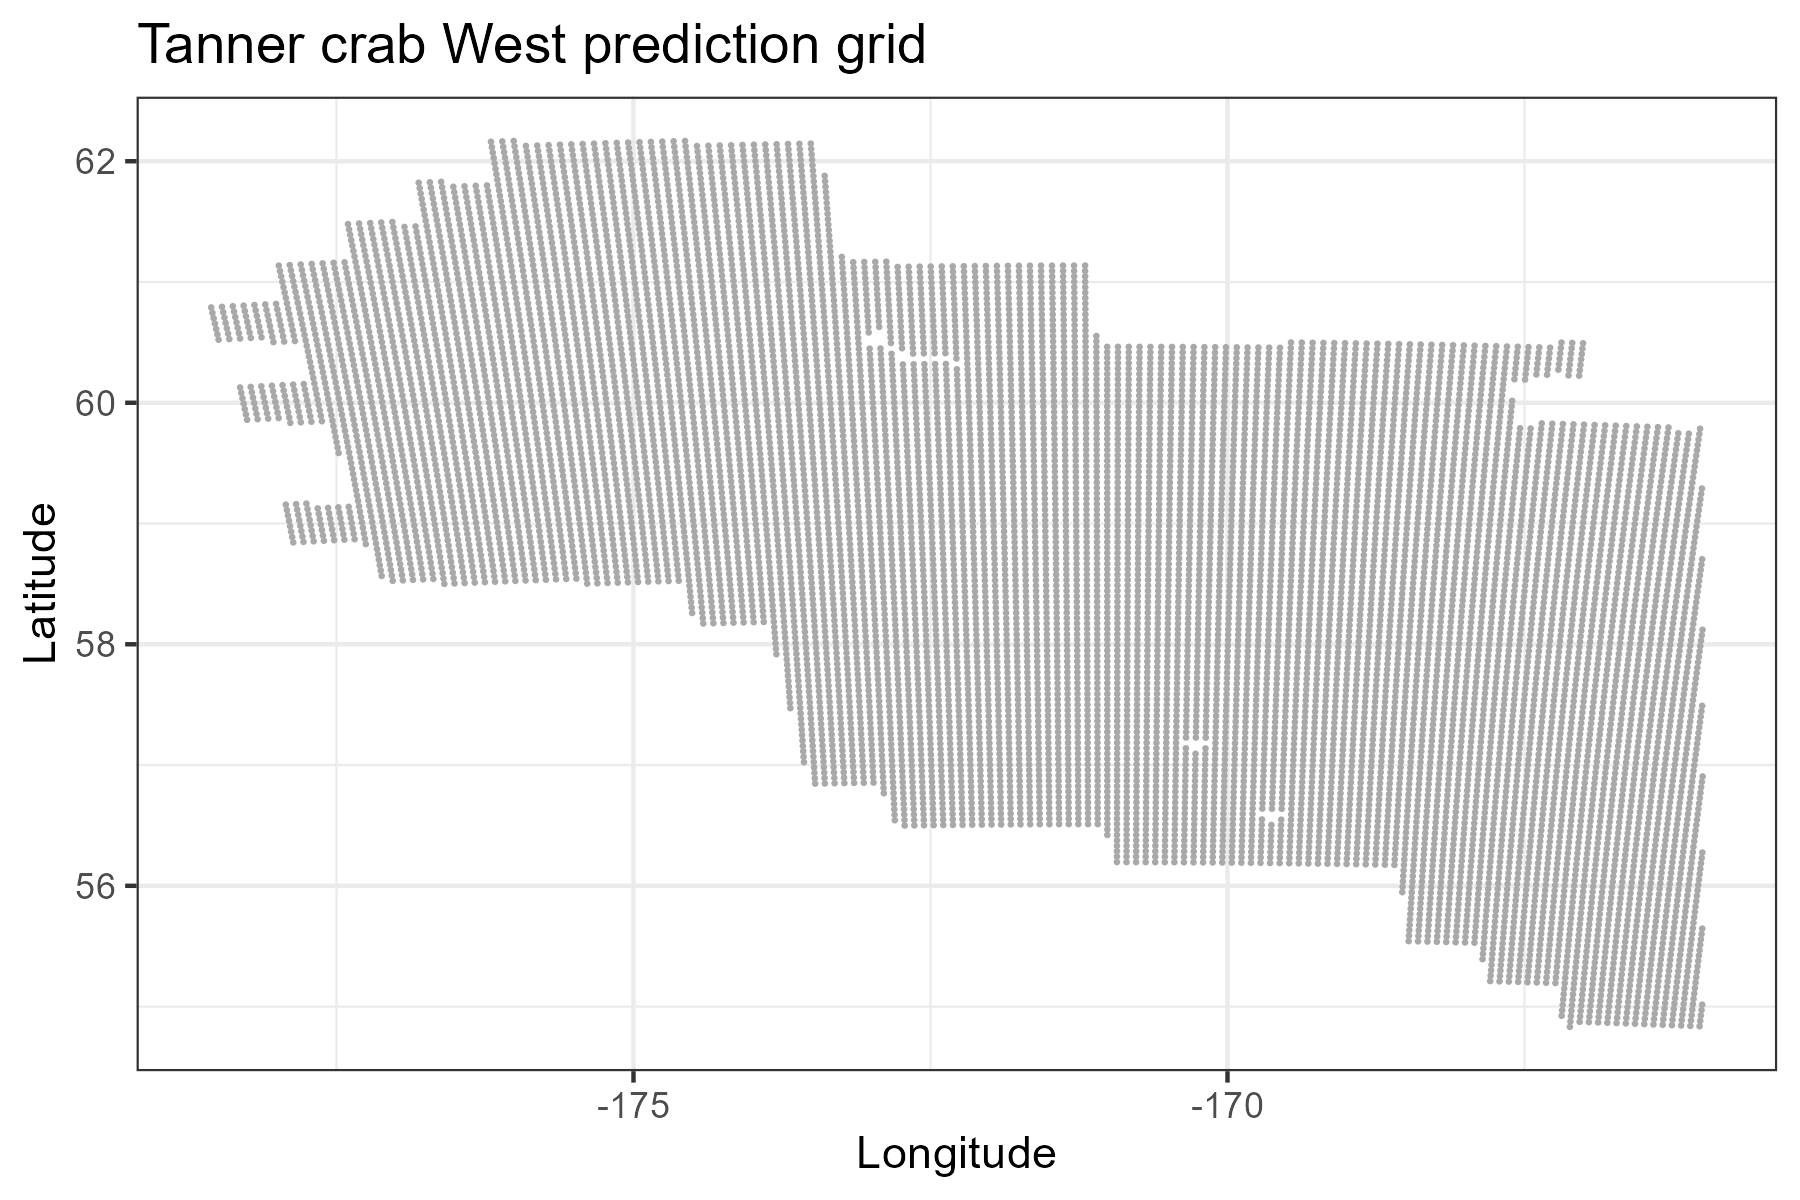
\includegraphics[width=6in]{../BAIRDI/Figures/west_predgrid} 

}

\caption{Prediction grid used to predict spatial abundance and biomass for Tanner crab west of 166°. Spatial resolution is 5km$^2$ and does not include land.}\label{fig:bairdi-west-grid}
\end{figure}

\begin{figure}

{\centering 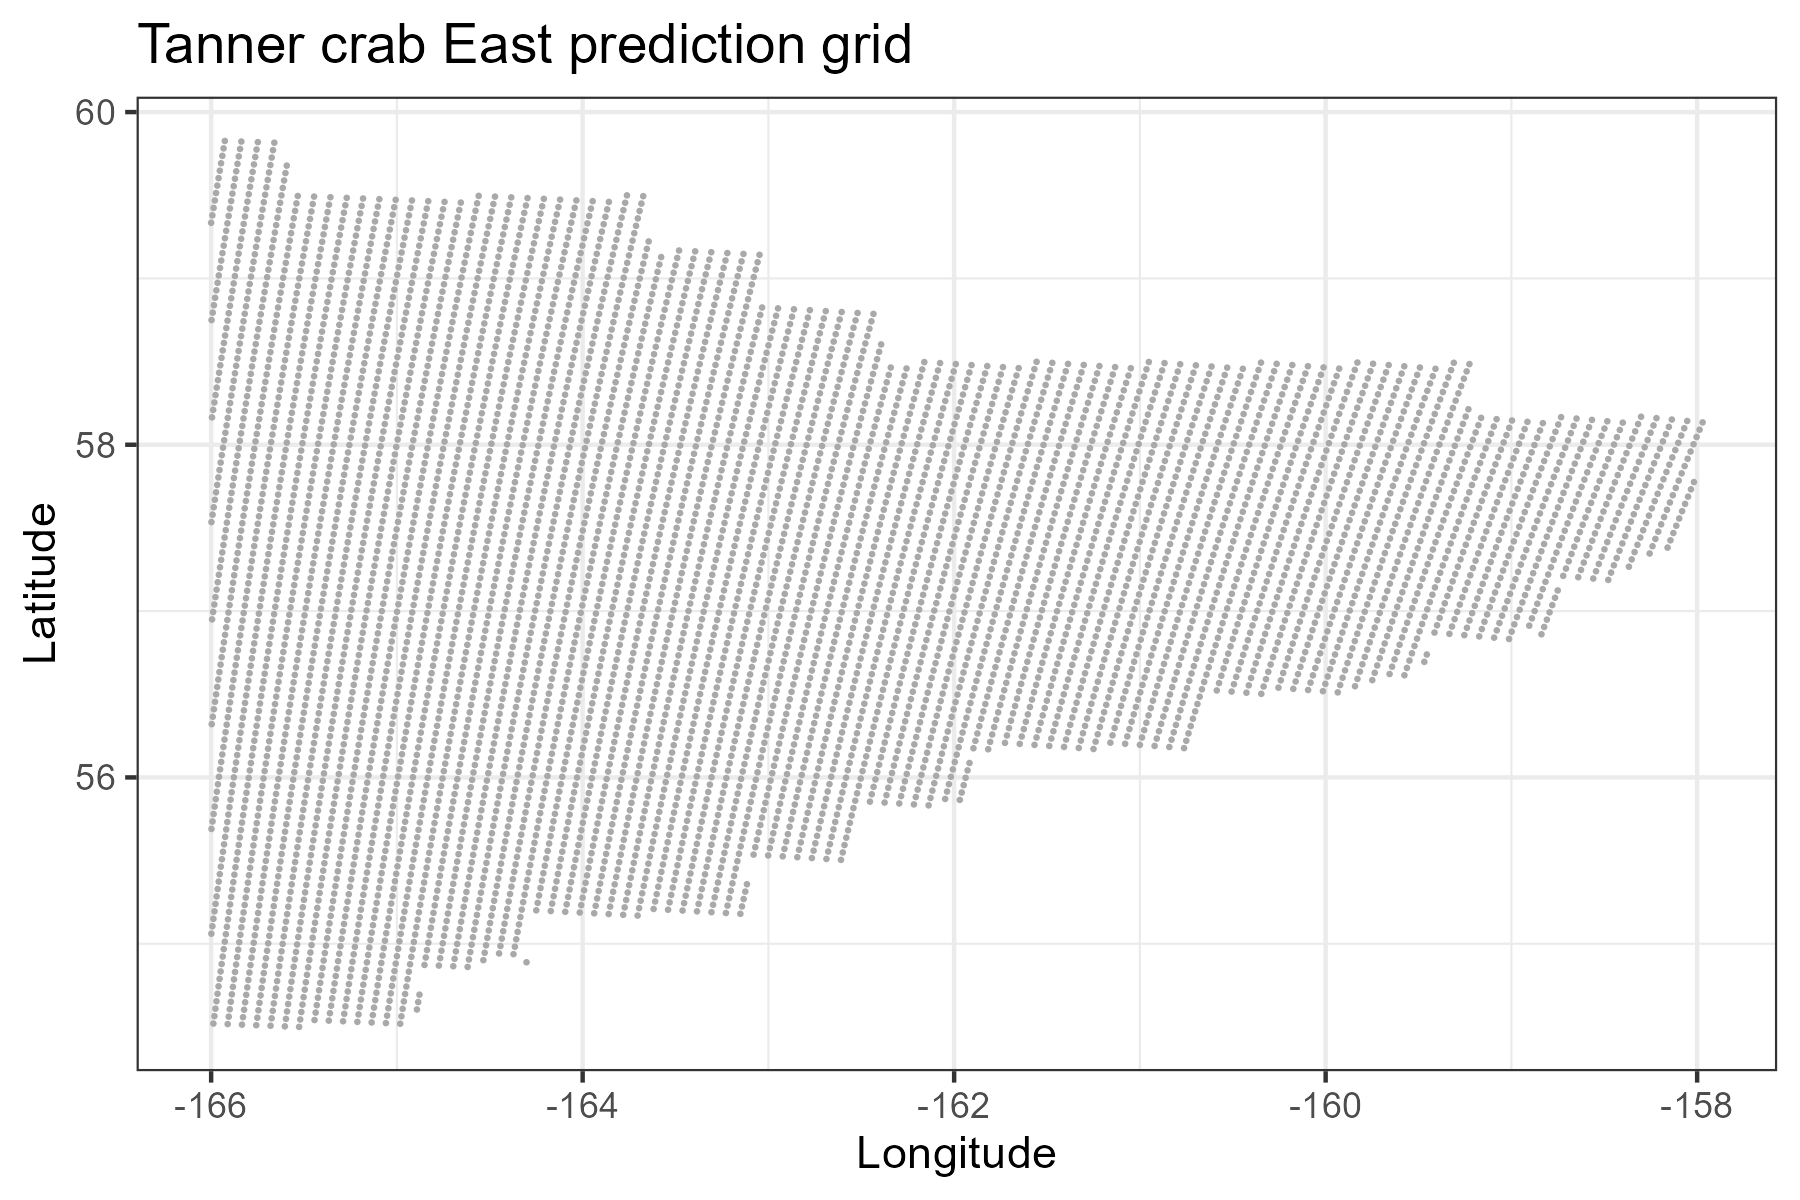
\includegraphics[width=6in]{../BAIRDI/Figures/east_predgrid} 

}

\caption{Prediction grid used to predict spatial abundance and biomass for Tanner crab east of 166°. Spatial resolution is 5km$^2$ and does not include land.}\label{fig:bairdi-east-grid}
\end{figure}

\begin{figure}

{\centering 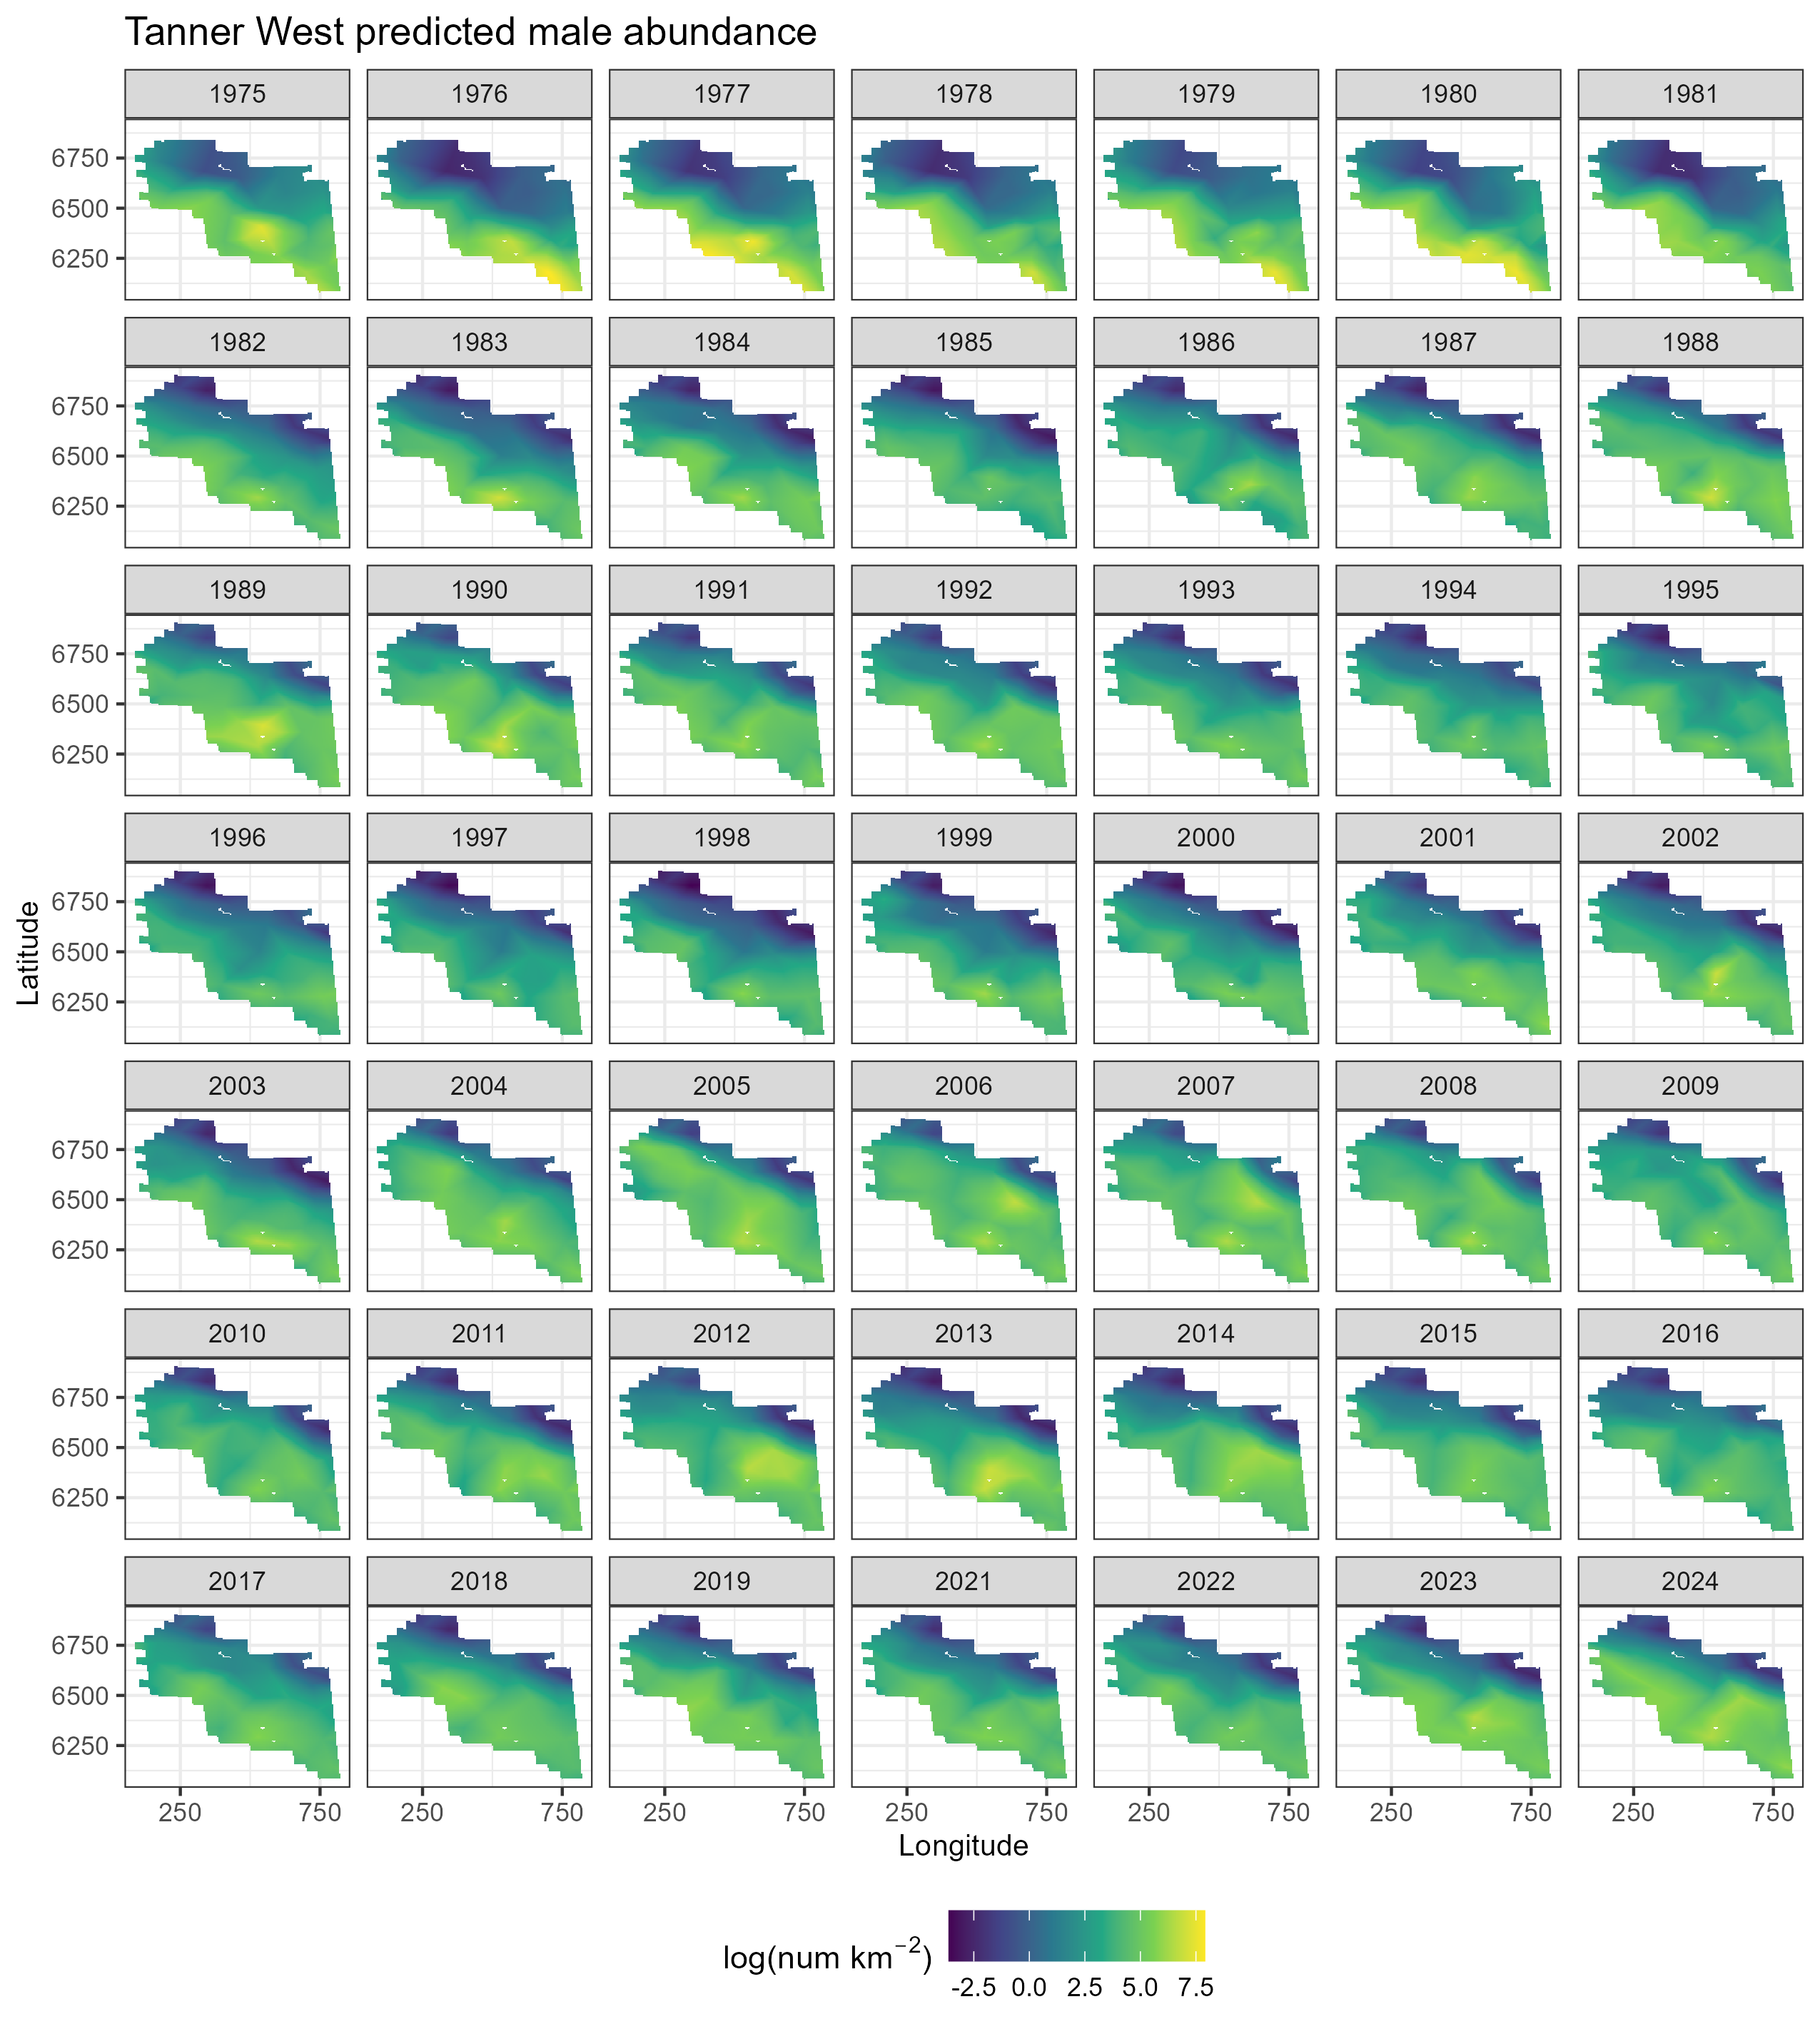
\includegraphics[width=1\linewidth,height=1\textheight]{../BAIRDI/Figures/TannerW_male_spatabund} 

}

\caption{Spatial predictions of male abundance west of 166° using NMFS summer bottom trawl survey data before 1982 and 1982 onward with a 50-knot mesh and a delta-gamma model family. Predictions from both of these periods/models are combined in this figure.}\label{fig:spatpred-abund-50-maleW}
\end{figure}

\begin{figure}

{\centering 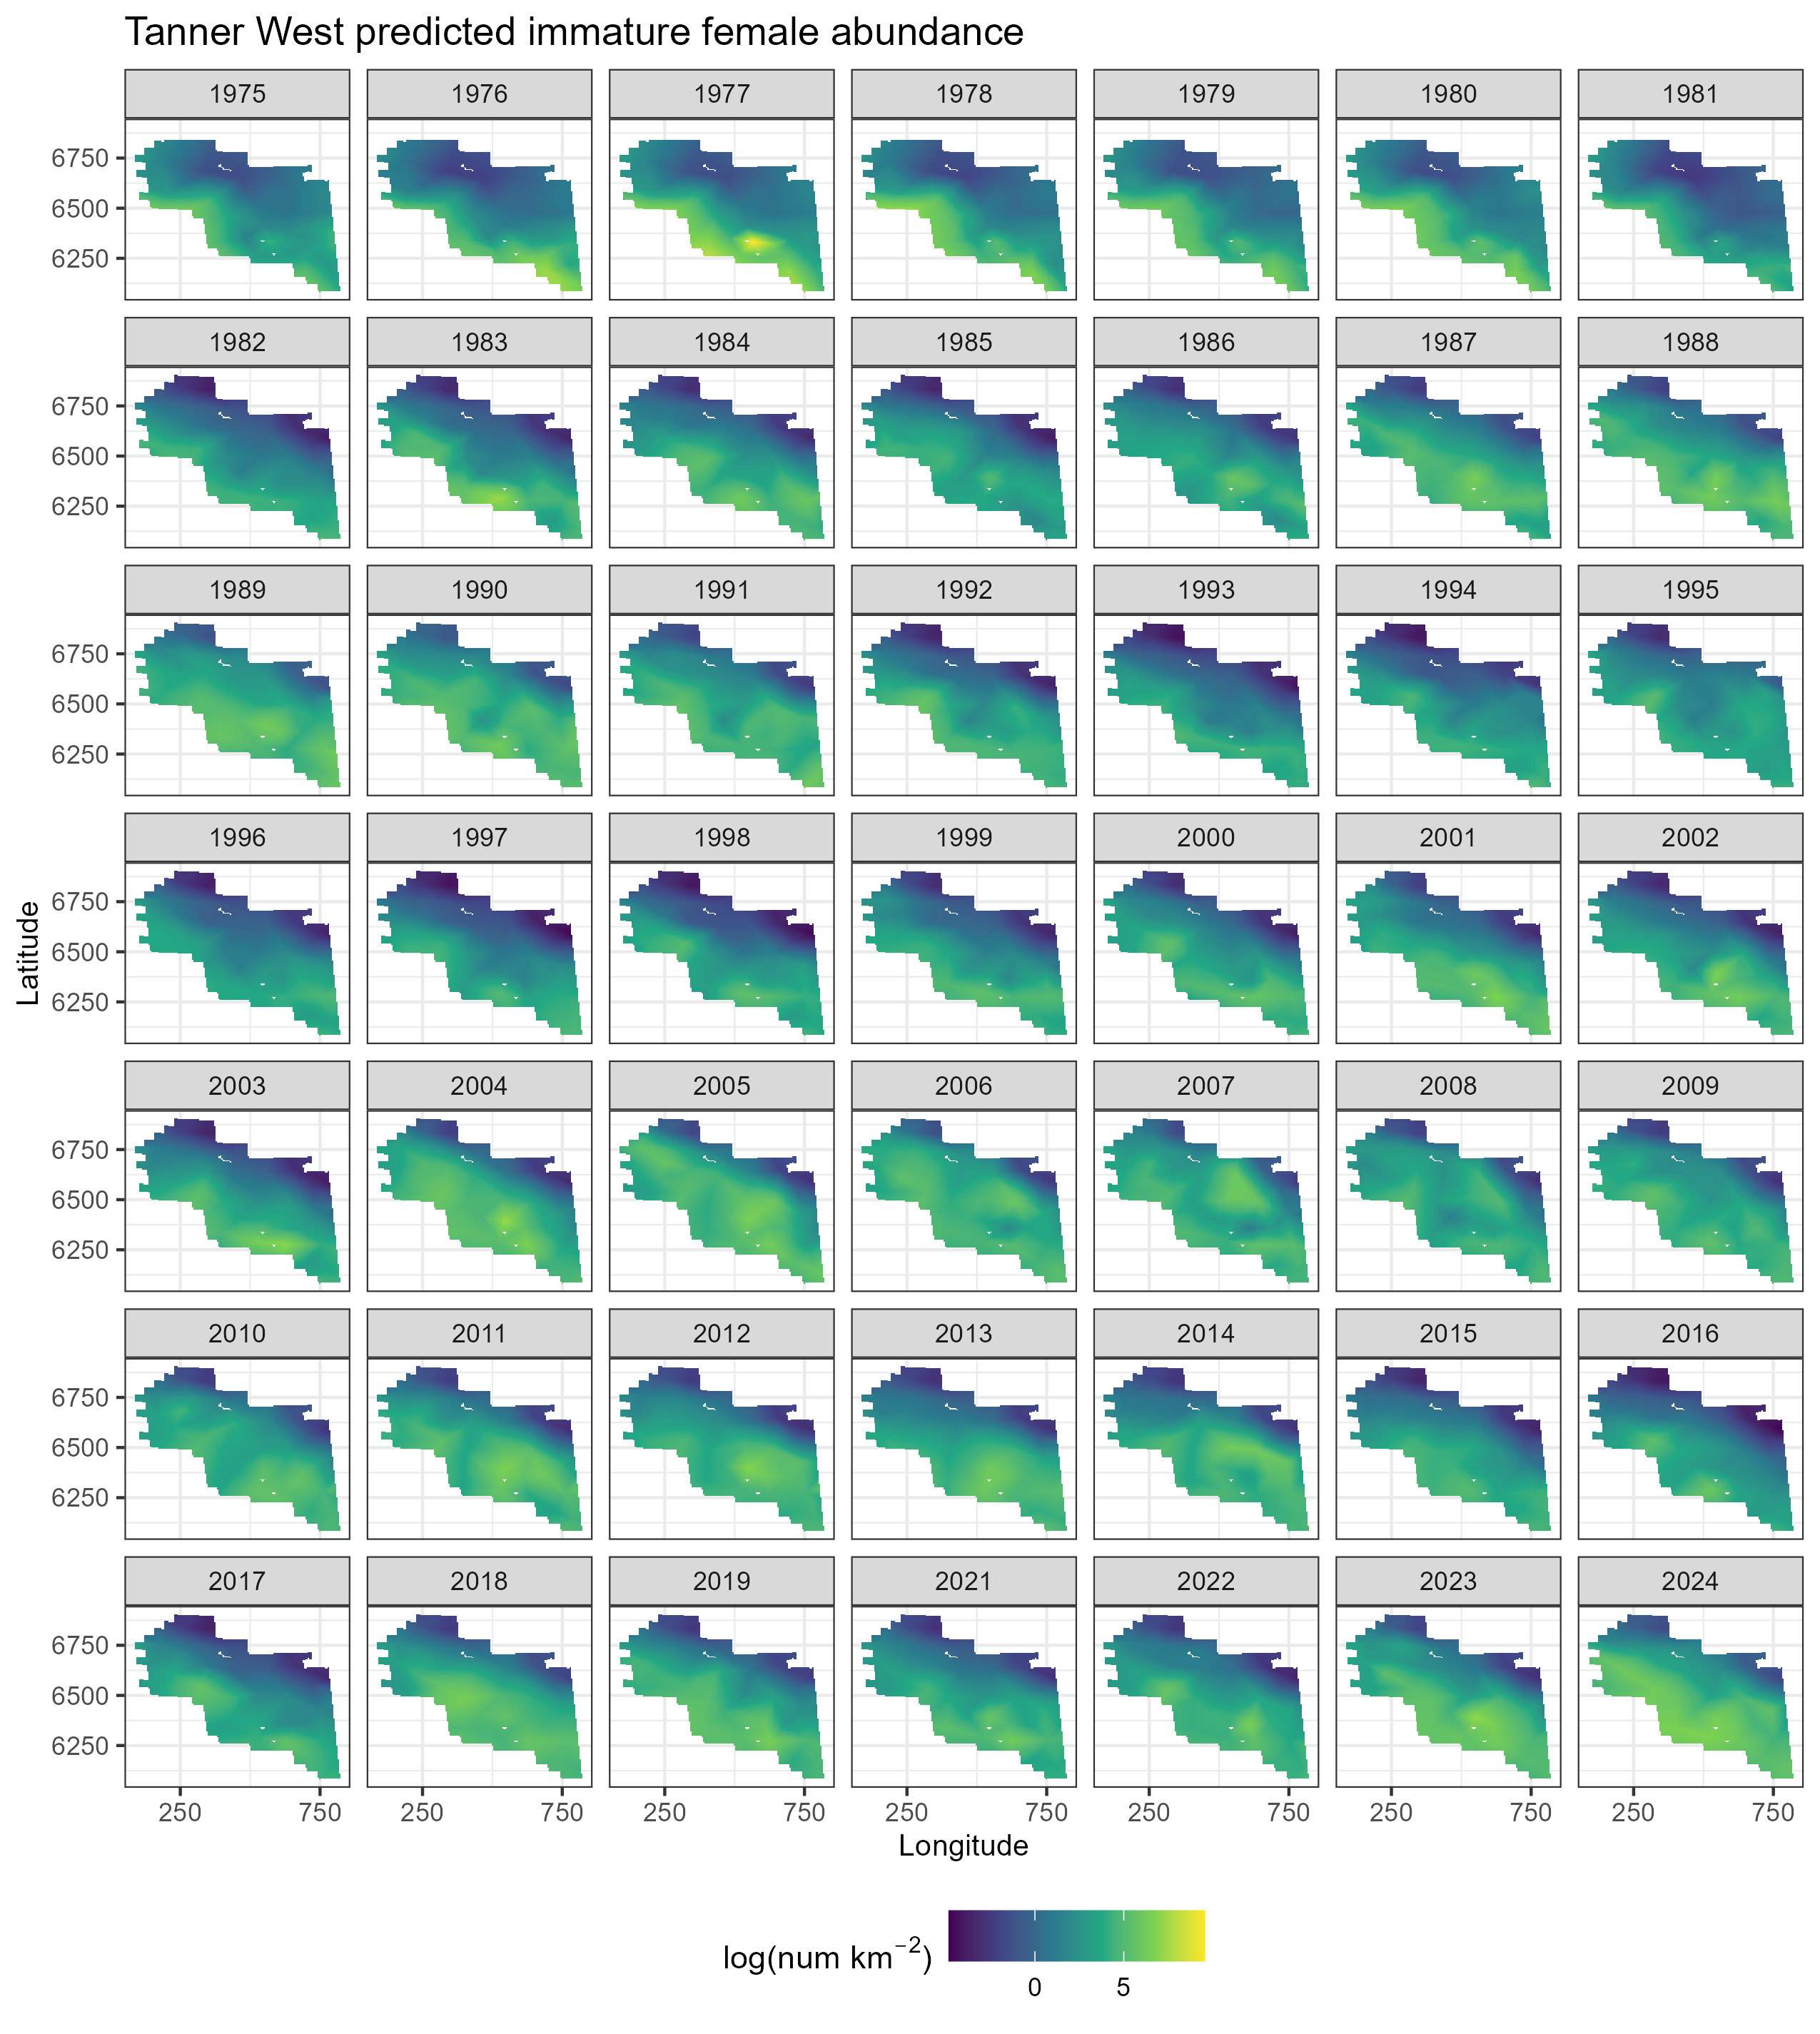
\includegraphics[width=1\linewidth,height=1\textheight]{../BAIRDI/Figures/TannerW_imfem_spatabund} 

}

\caption{Spatial predictions of immature female abundance west of 166° using NMFS summer bottom trawl survey data before 1982 and 1982 onward with a 50-knot mesh and a delta-gamma model family. Predictions from both of these periods/models are combined in this figure.}\label{fig:spatpred-abund-50-imfemW}
\end{figure}

\begin{figure}

{\centering 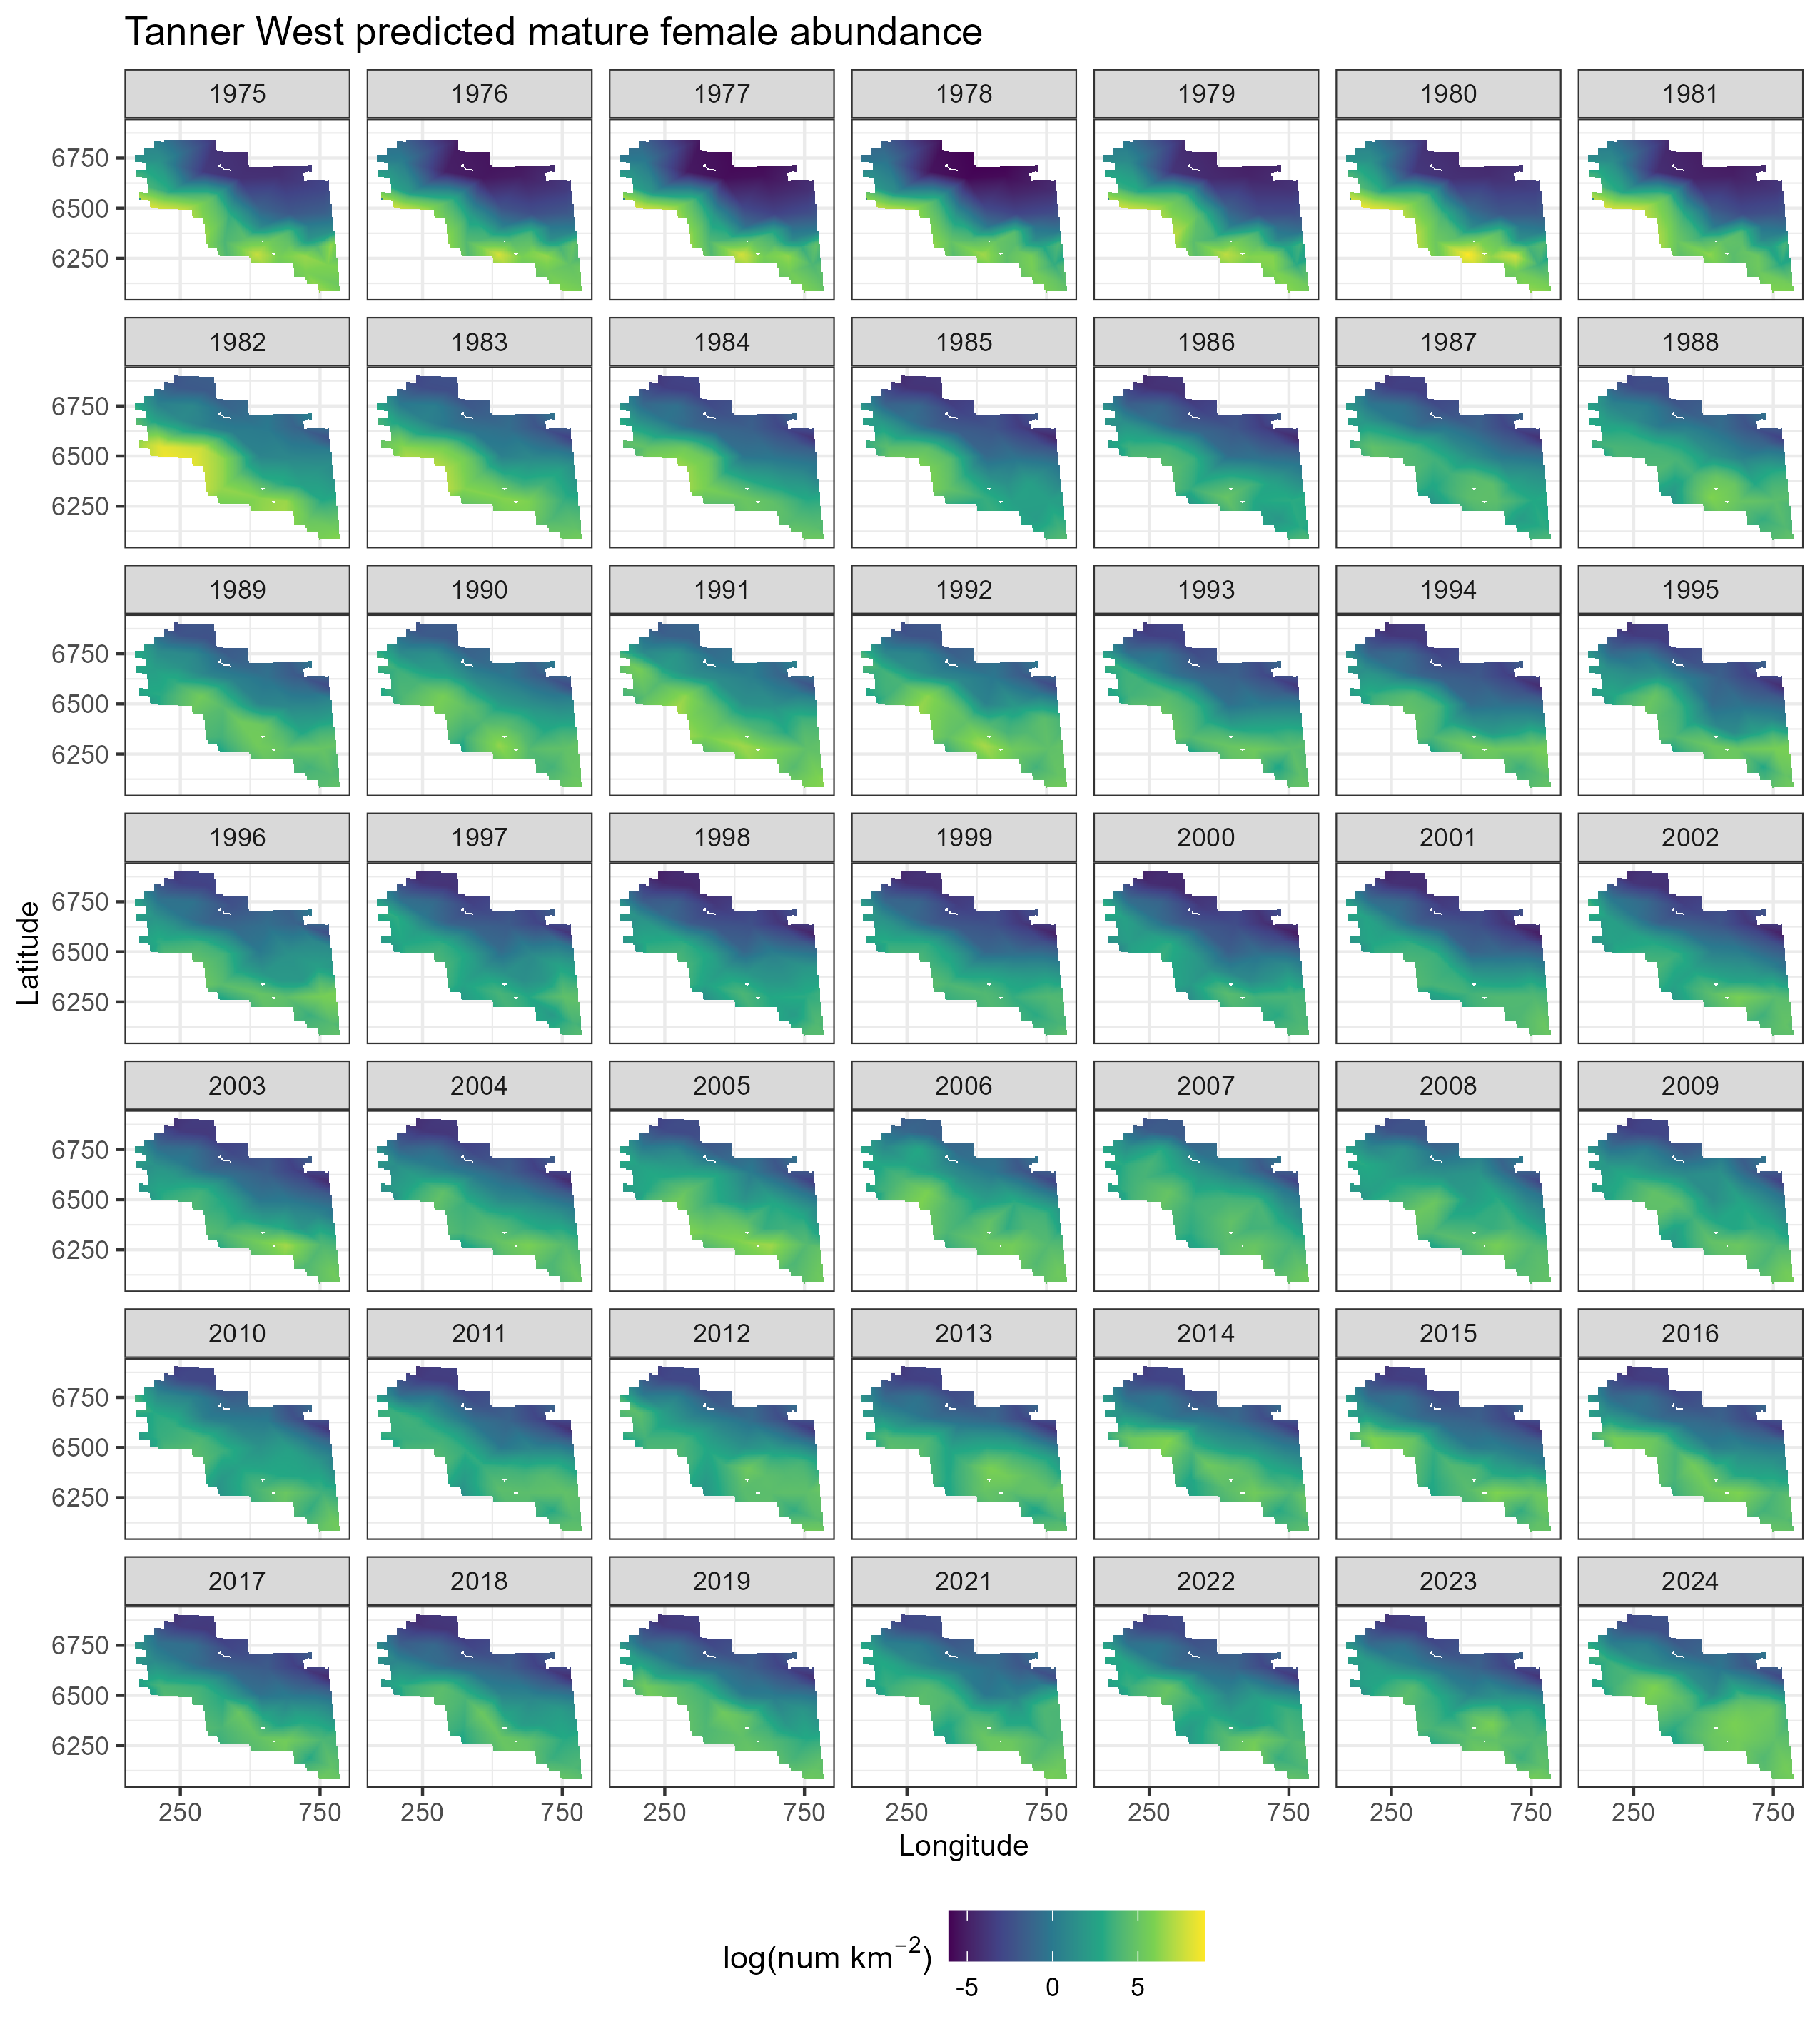
\includegraphics[width=1\linewidth,height=1\textheight]{../BAIRDI/Figures/TannerW_matfem_spatabund} 

}

\caption{Spatial predictions of mature female abundance west of 166° using NMFS summer bottom trawl survey data before 1982 and 1982 onward with a 50-knot mesh and a delta-gamma model family. Predictions from both of these periods/models are combined in this figure.}\label{fig:spatpred-abund-50-matfemW}
\end{figure}

\begin{figure}

{\centering 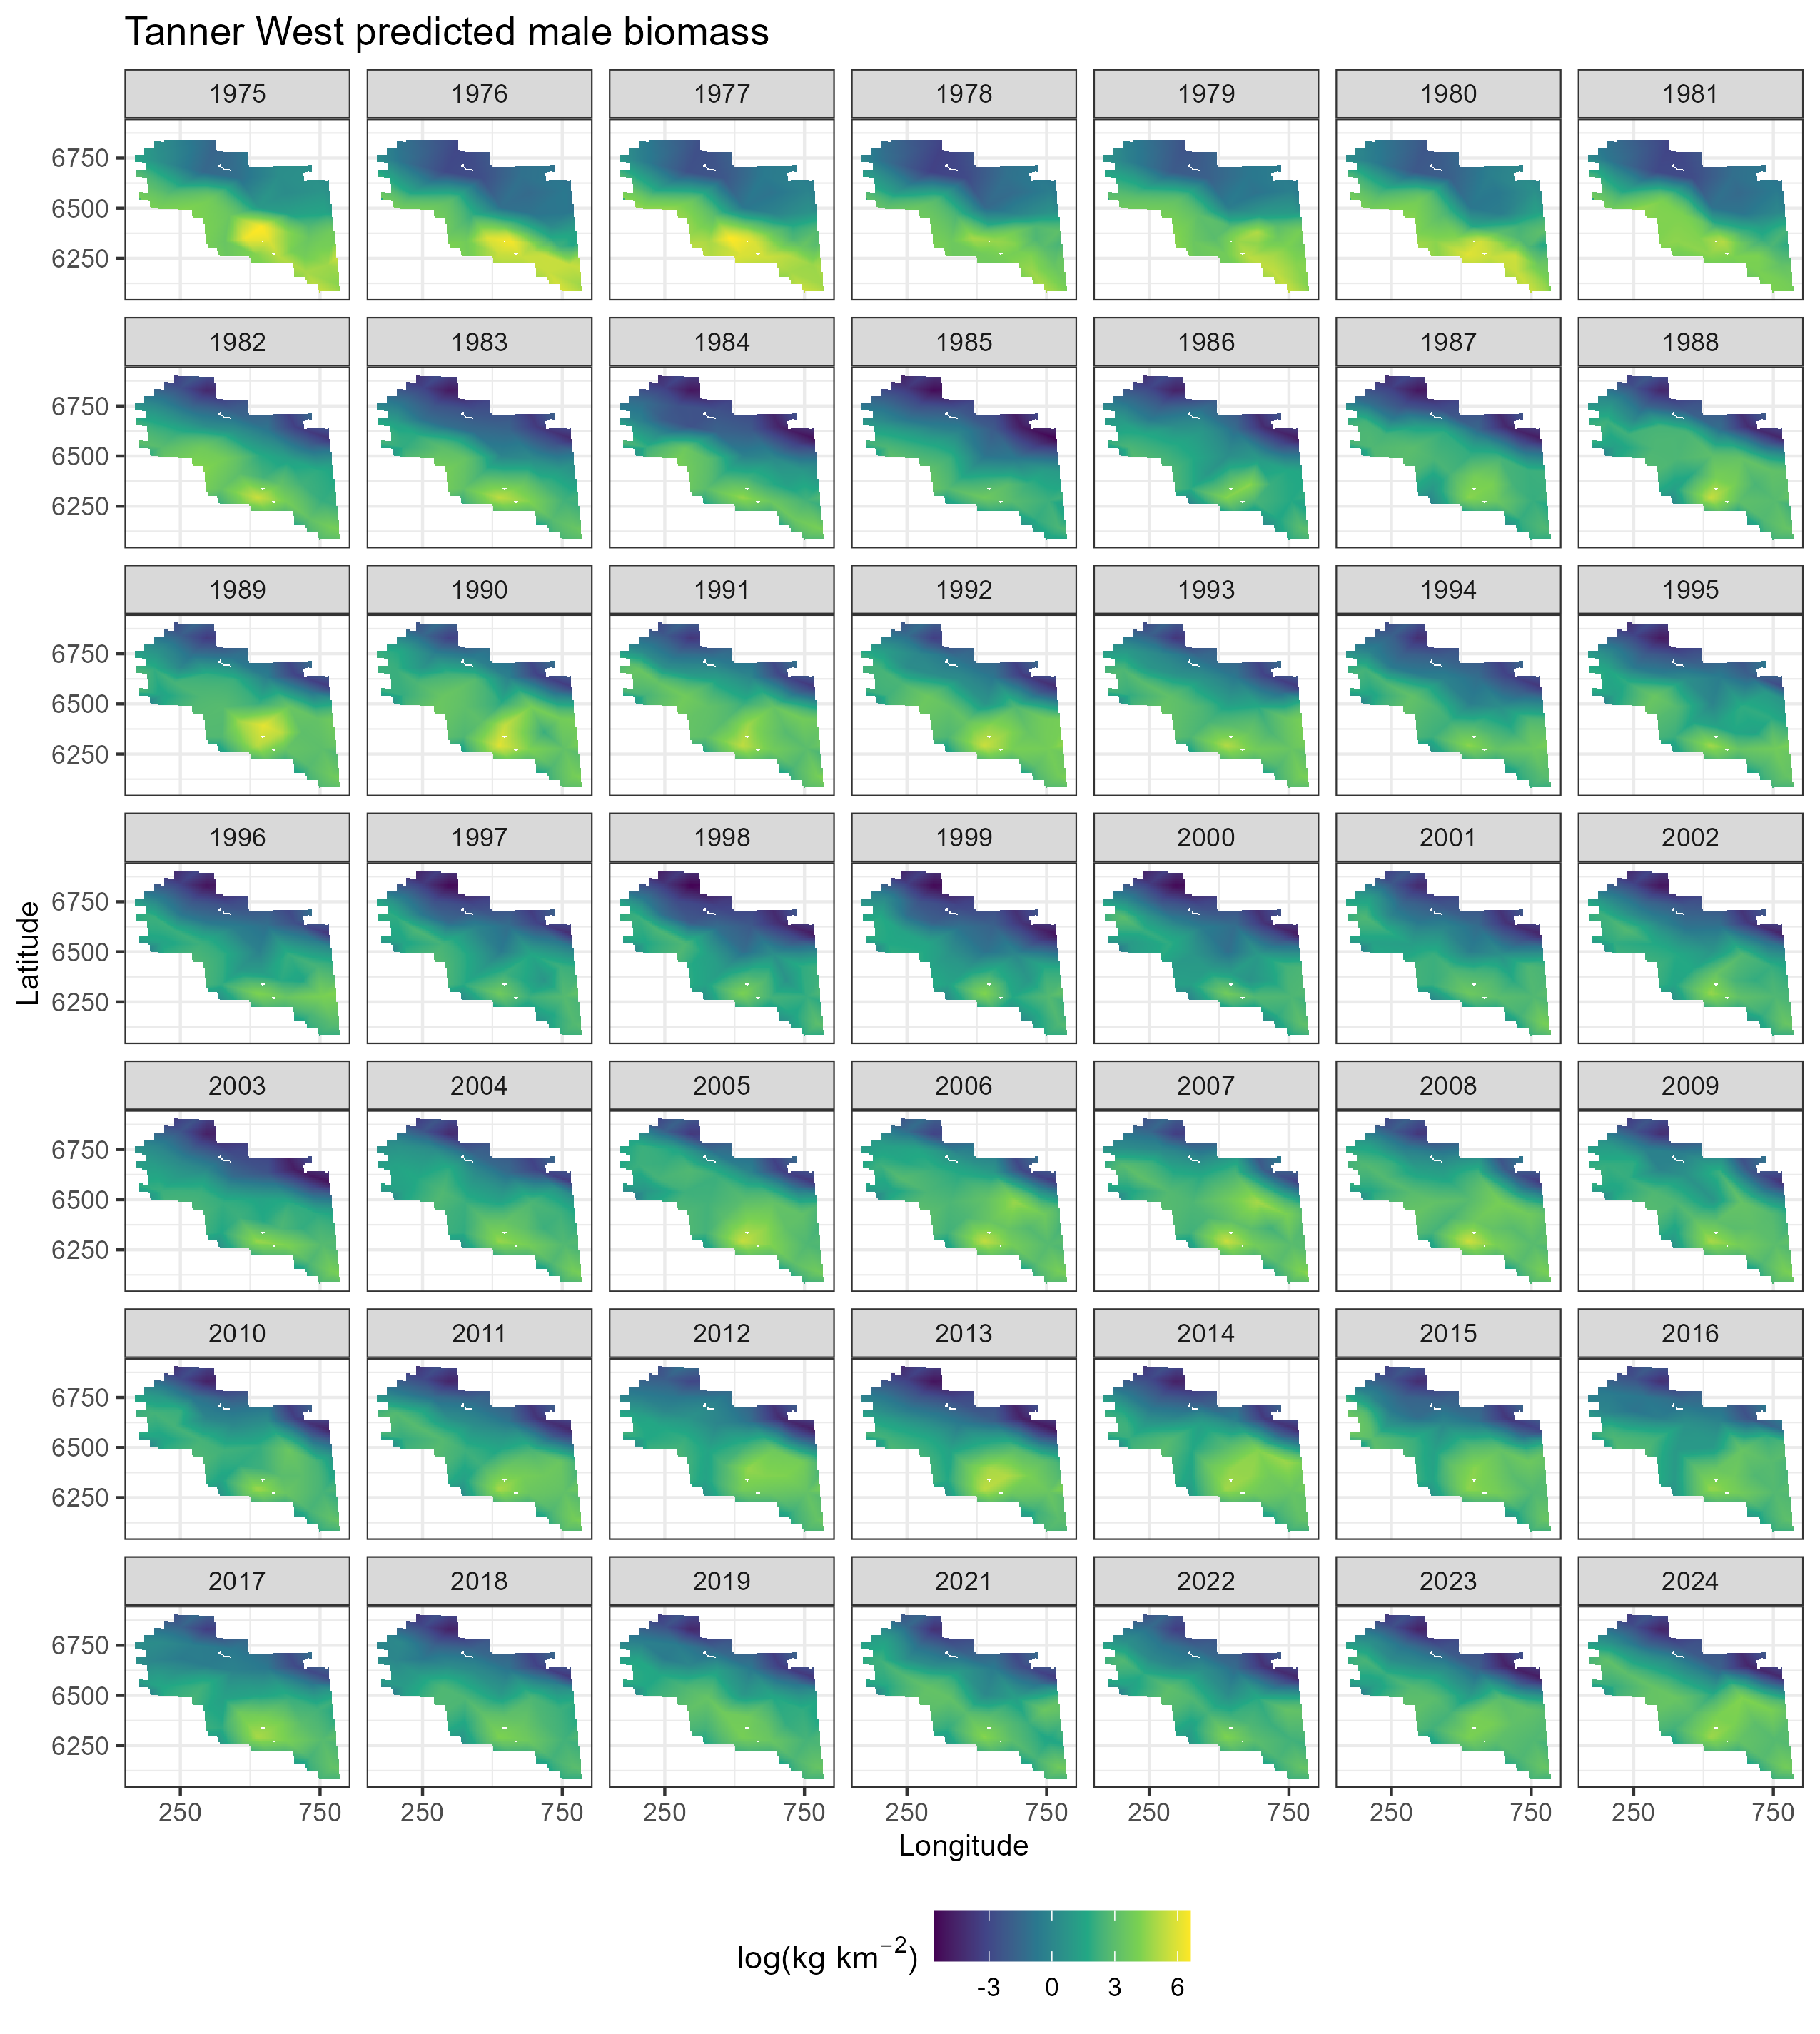
\includegraphics[width=1\linewidth,height=1\textheight]{../BAIRDI/Figures/TannerW_male_spatbio} 

}

\caption{Spatial predictions of male biomass west of 166° using NMFS summer bottom trawl survey data before 1982 and 1982 onward with a 50-knot mesh and a delta-gamma model family. Predictions from both of these periods/models are combined in this figure.}\label{fig:spatpred-bio-50-maleW}
\end{figure}

\begin{figure}

{\centering 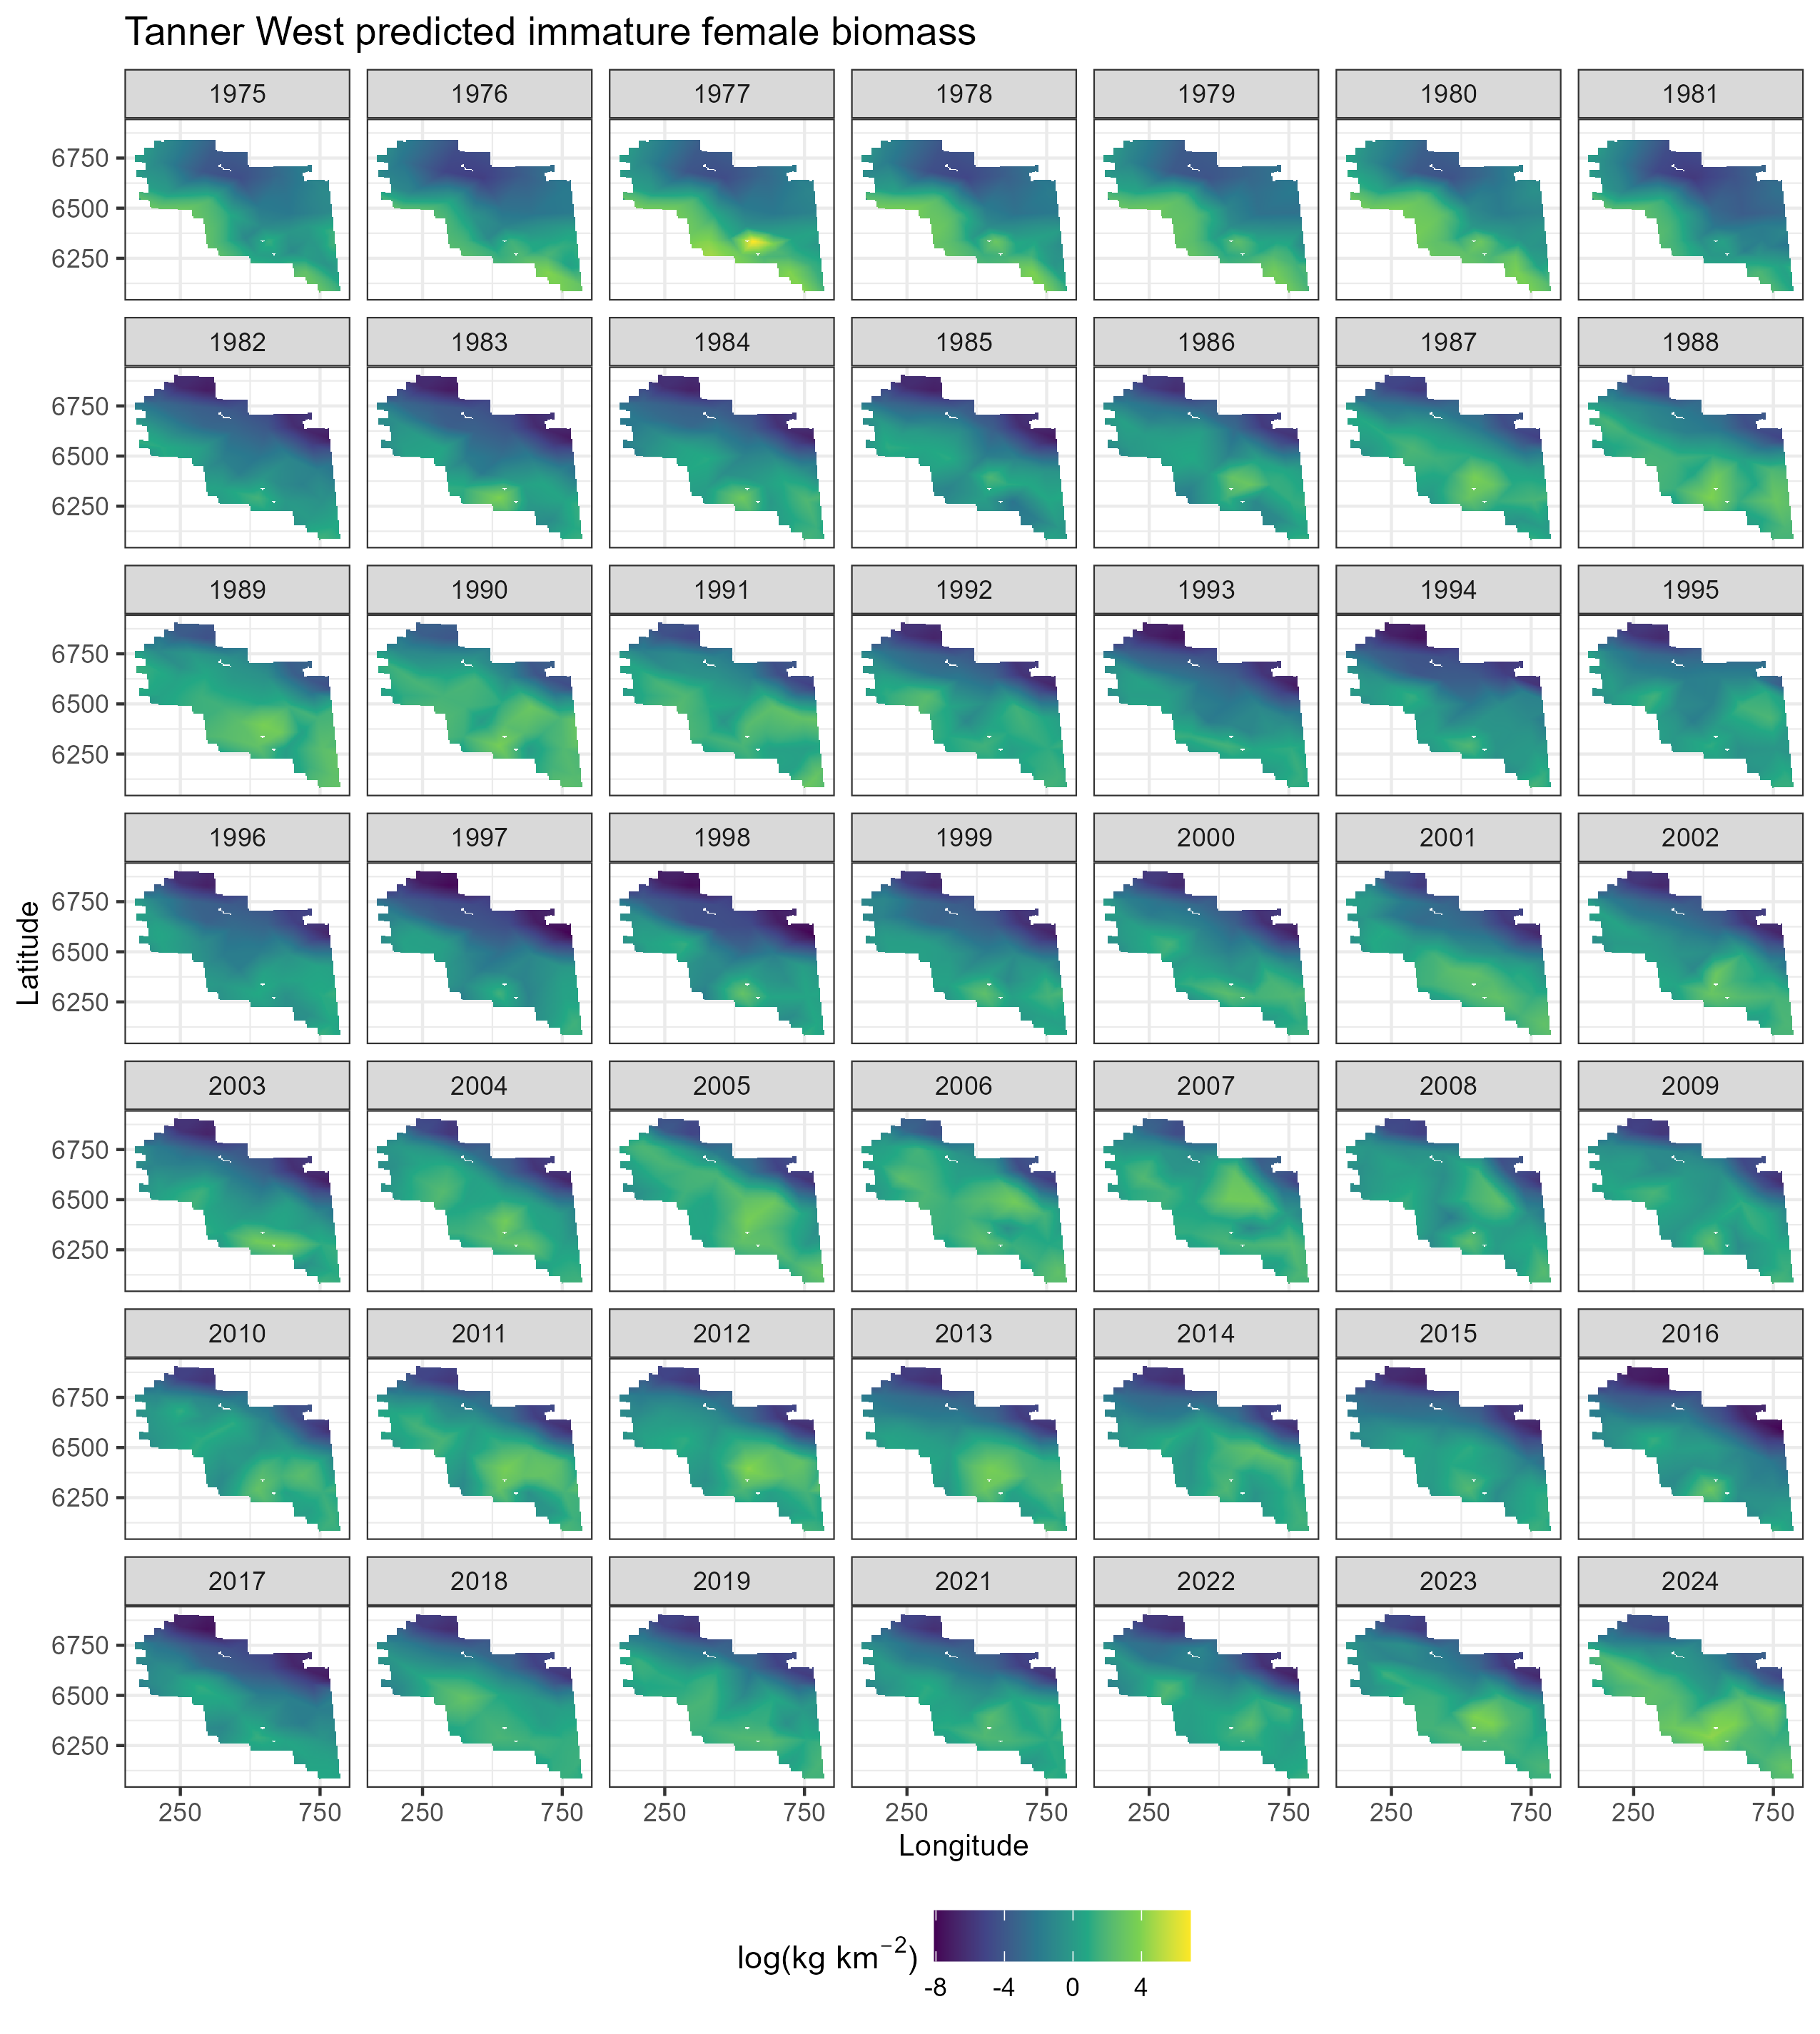
\includegraphics[width=1\linewidth,height=1\textheight]{../BAIRDI/Figures/TannerW_imfem_spatbio} 

}

\caption{Spatial predictions of immature female biomass west of 166° using NMFS summer bottom trawl survey data before 1982 and 1982 onward with a 50-knot mesh and a delta-gamma model family. Predictions from both of these periods/models are combined in this figure.}\label{fig:spatpred-bio-50-imfemW}
\end{figure}

\begin{figure}

{\centering 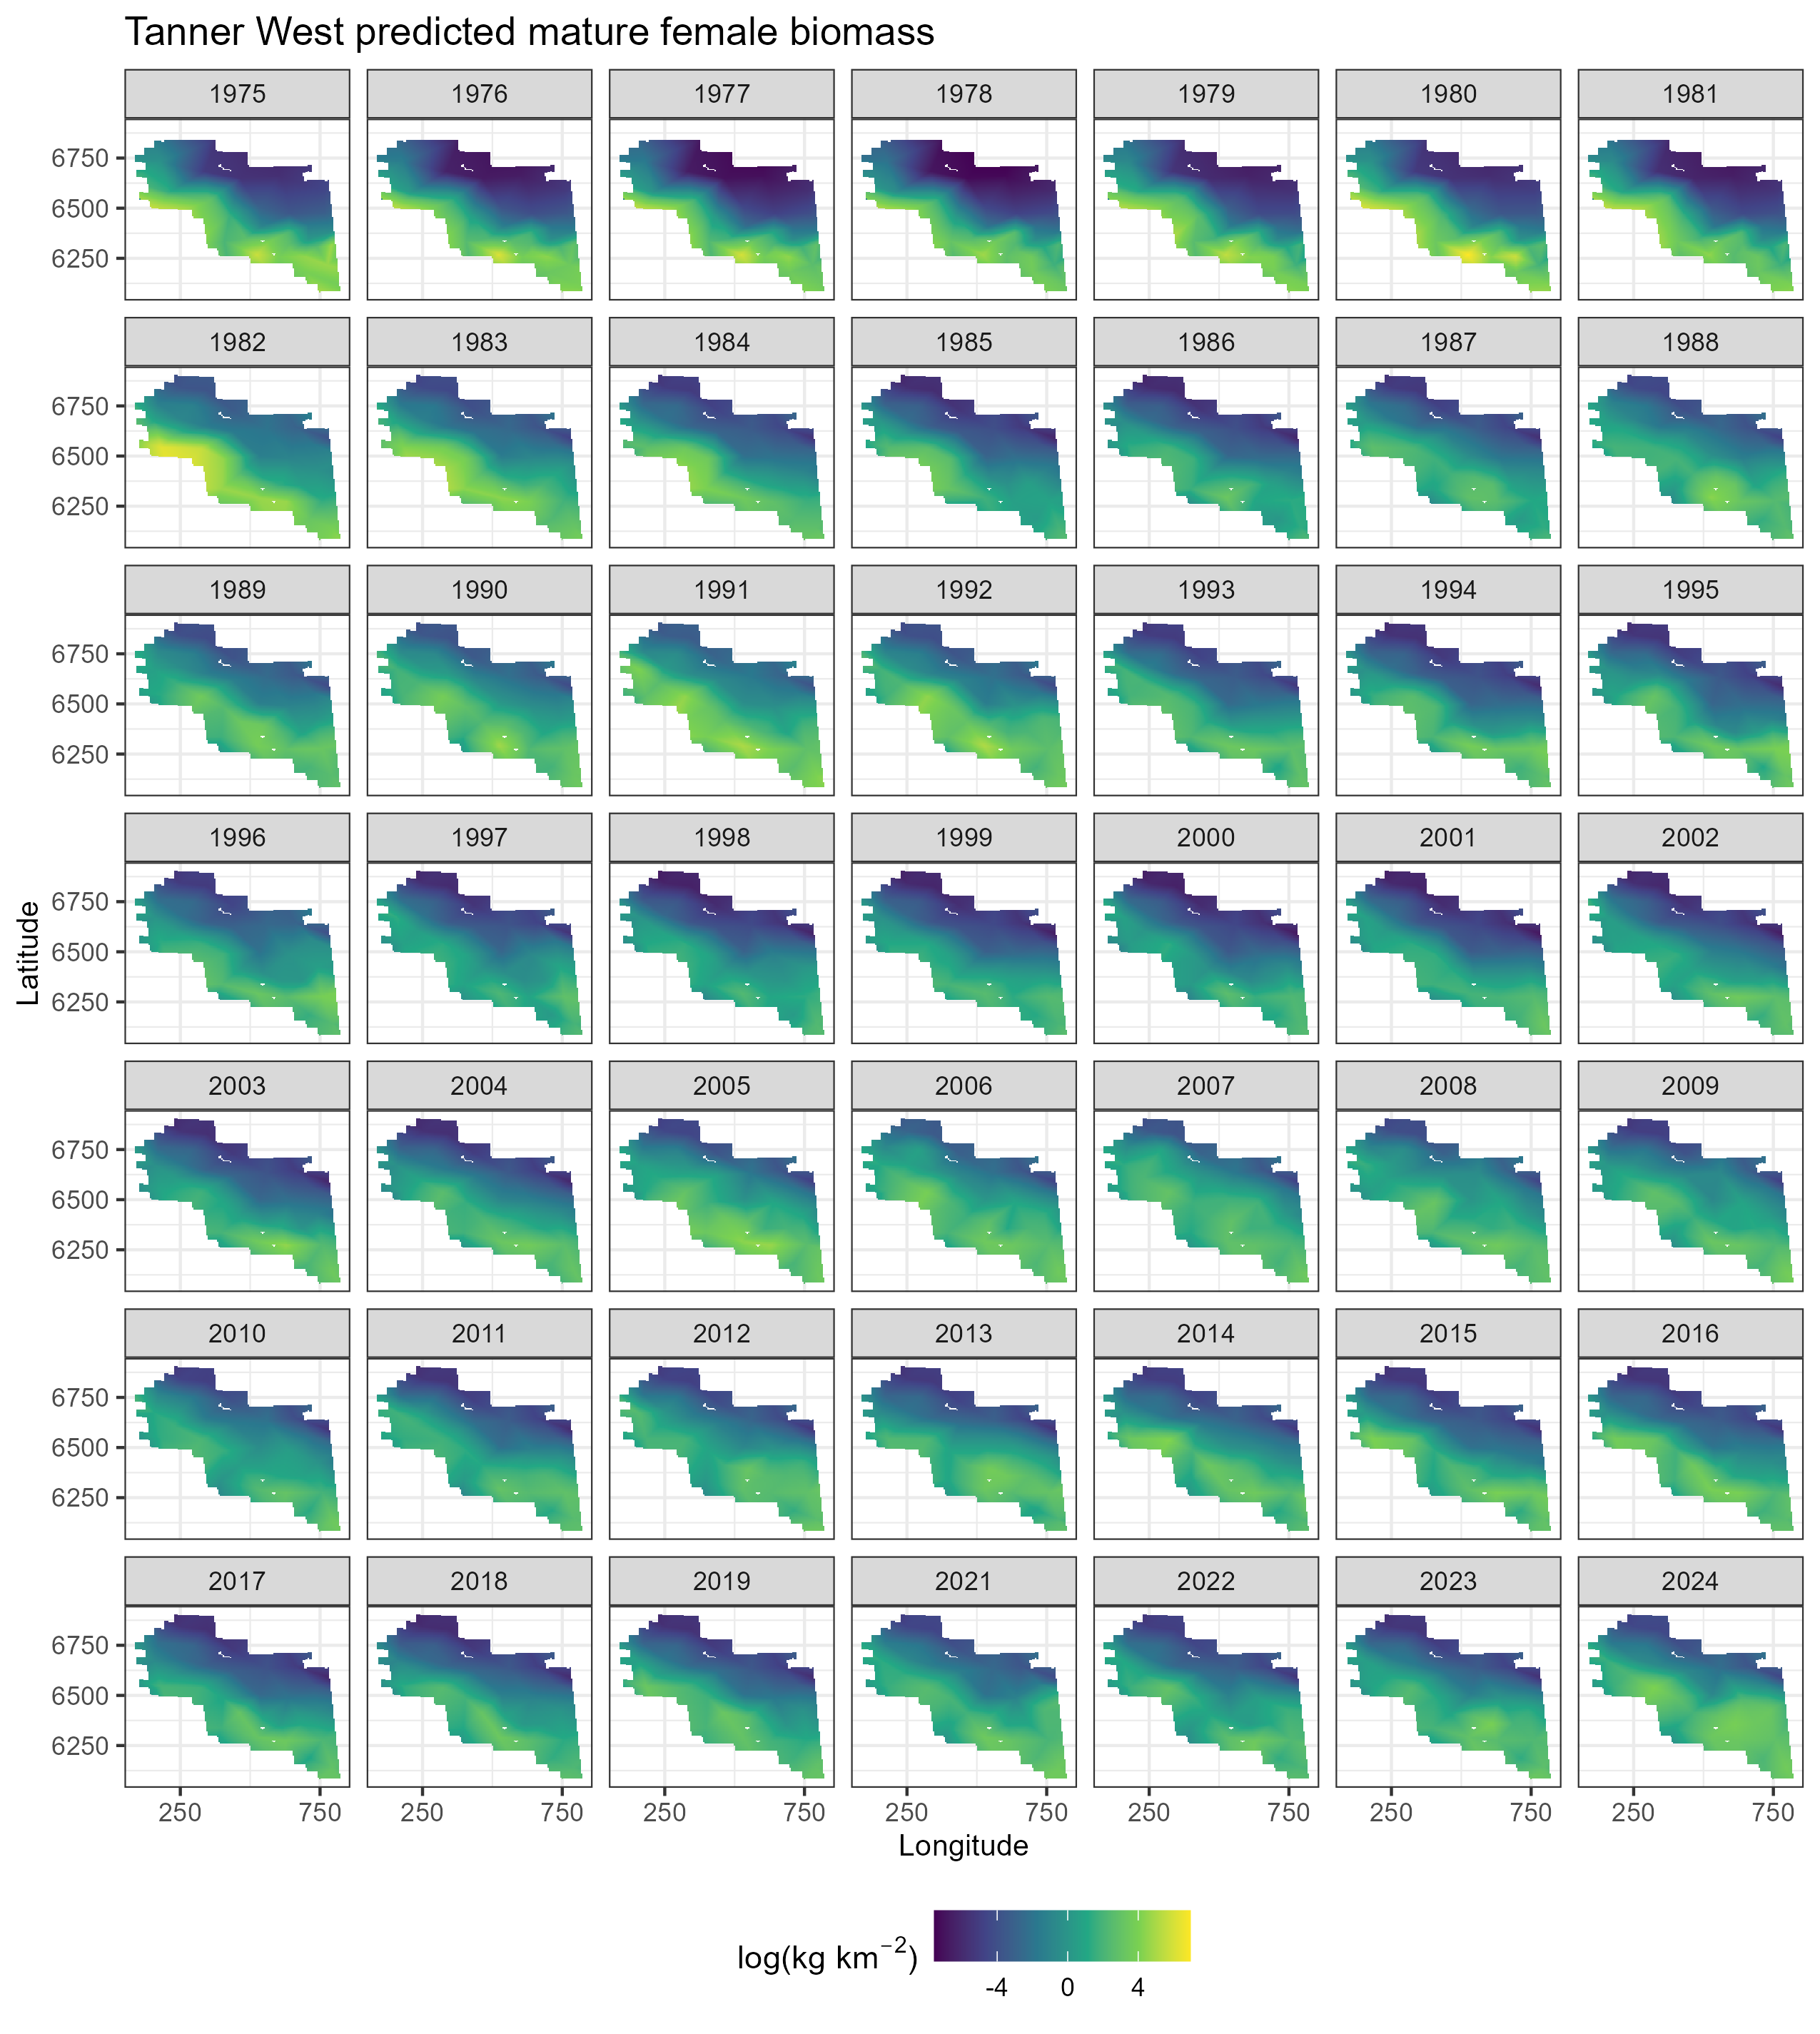
\includegraphics[width=1\linewidth,height=1\textheight]{../BAIRDI/Figures/TannerW_matfem_spatbio} 

}

\caption{Spatial predictions of mature female biomass west of 166° using NMFS summer bottom trawl survey data before 1982 and 1982 onward with a 50-knot mesh and a delta-gamma model family. Predictions from both of these periods/models are combined in this figure.}\label{fig:spatpred-bio-50-matfemW}
\end{figure}

\begin{figure}

{\centering 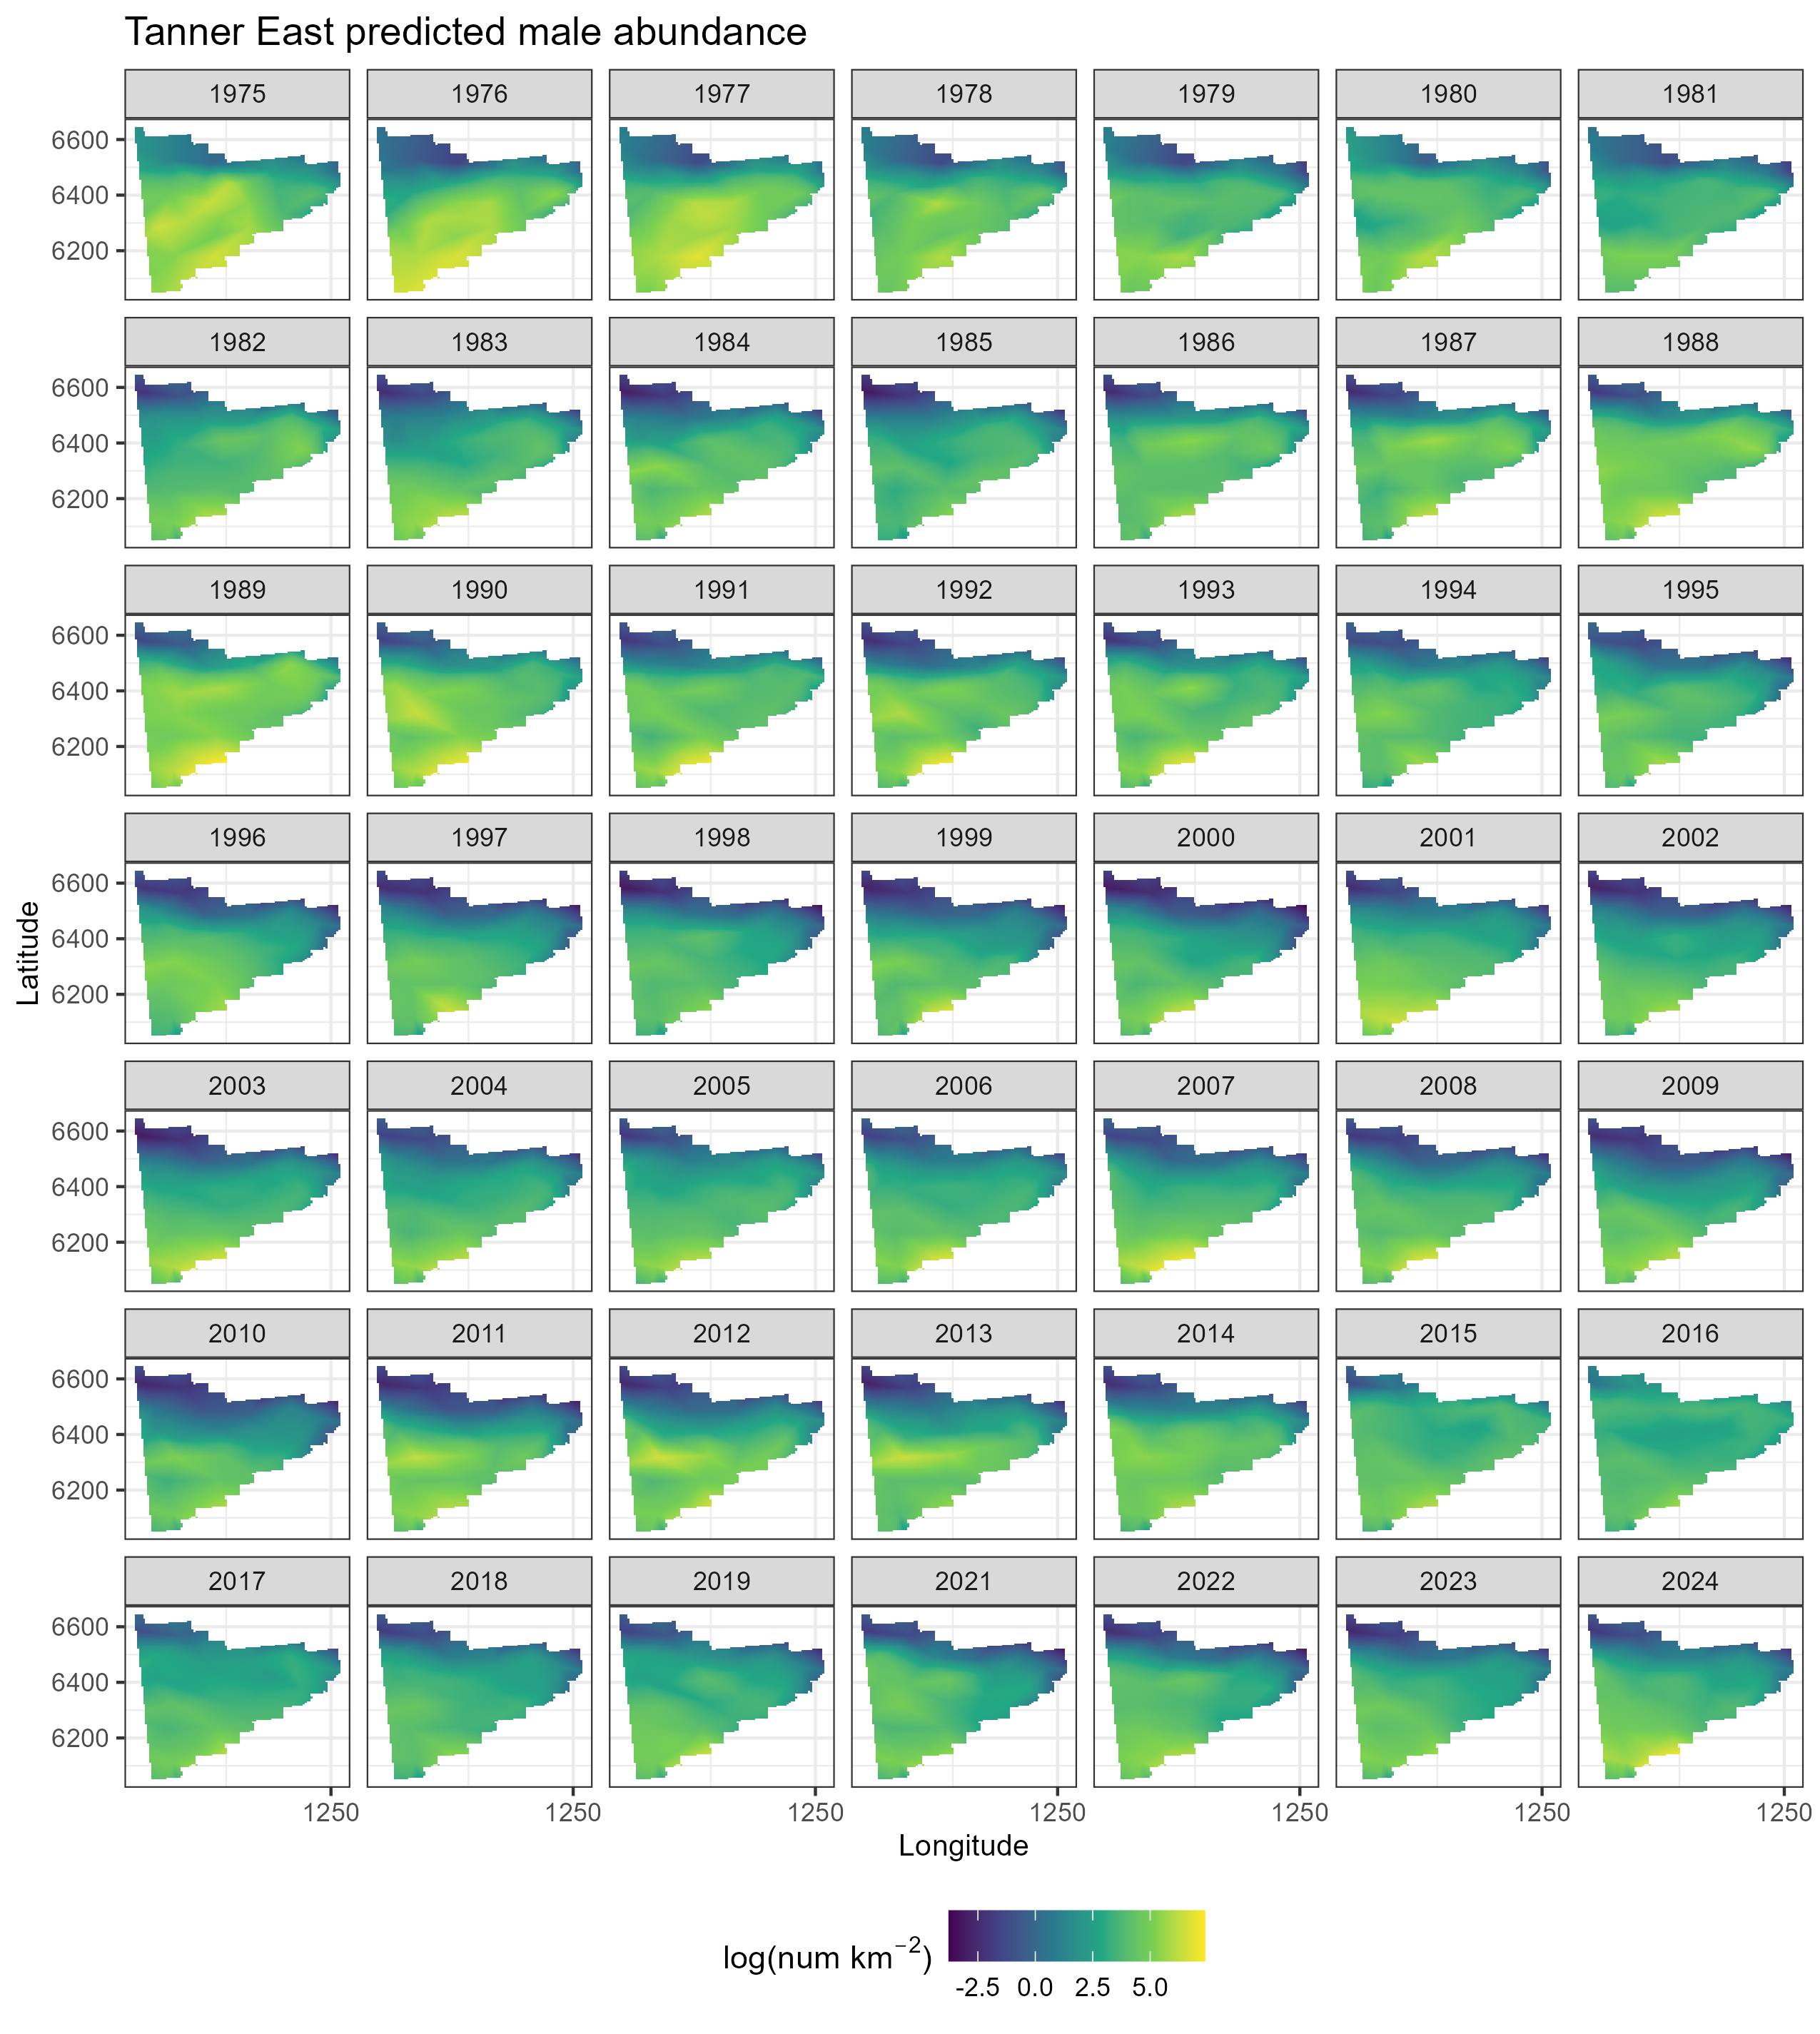
\includegraphics[width=1\linewidth,height=1\textheight]{../BAIRDI/Figures/TannerE_male_spatabund} 

}

\caption{Spatial predictions of male abundance east of 166° using NMFS summer bottom trawl survey data before 1982 and 1982 onward with a 50-knot mesh and a delta-gamma model family. Predictions from both of these periods/models are combined in this figure.}\label{fig:spatpred-abund-50-maleE}
\end{figure}

\begin{figure}

{\centering 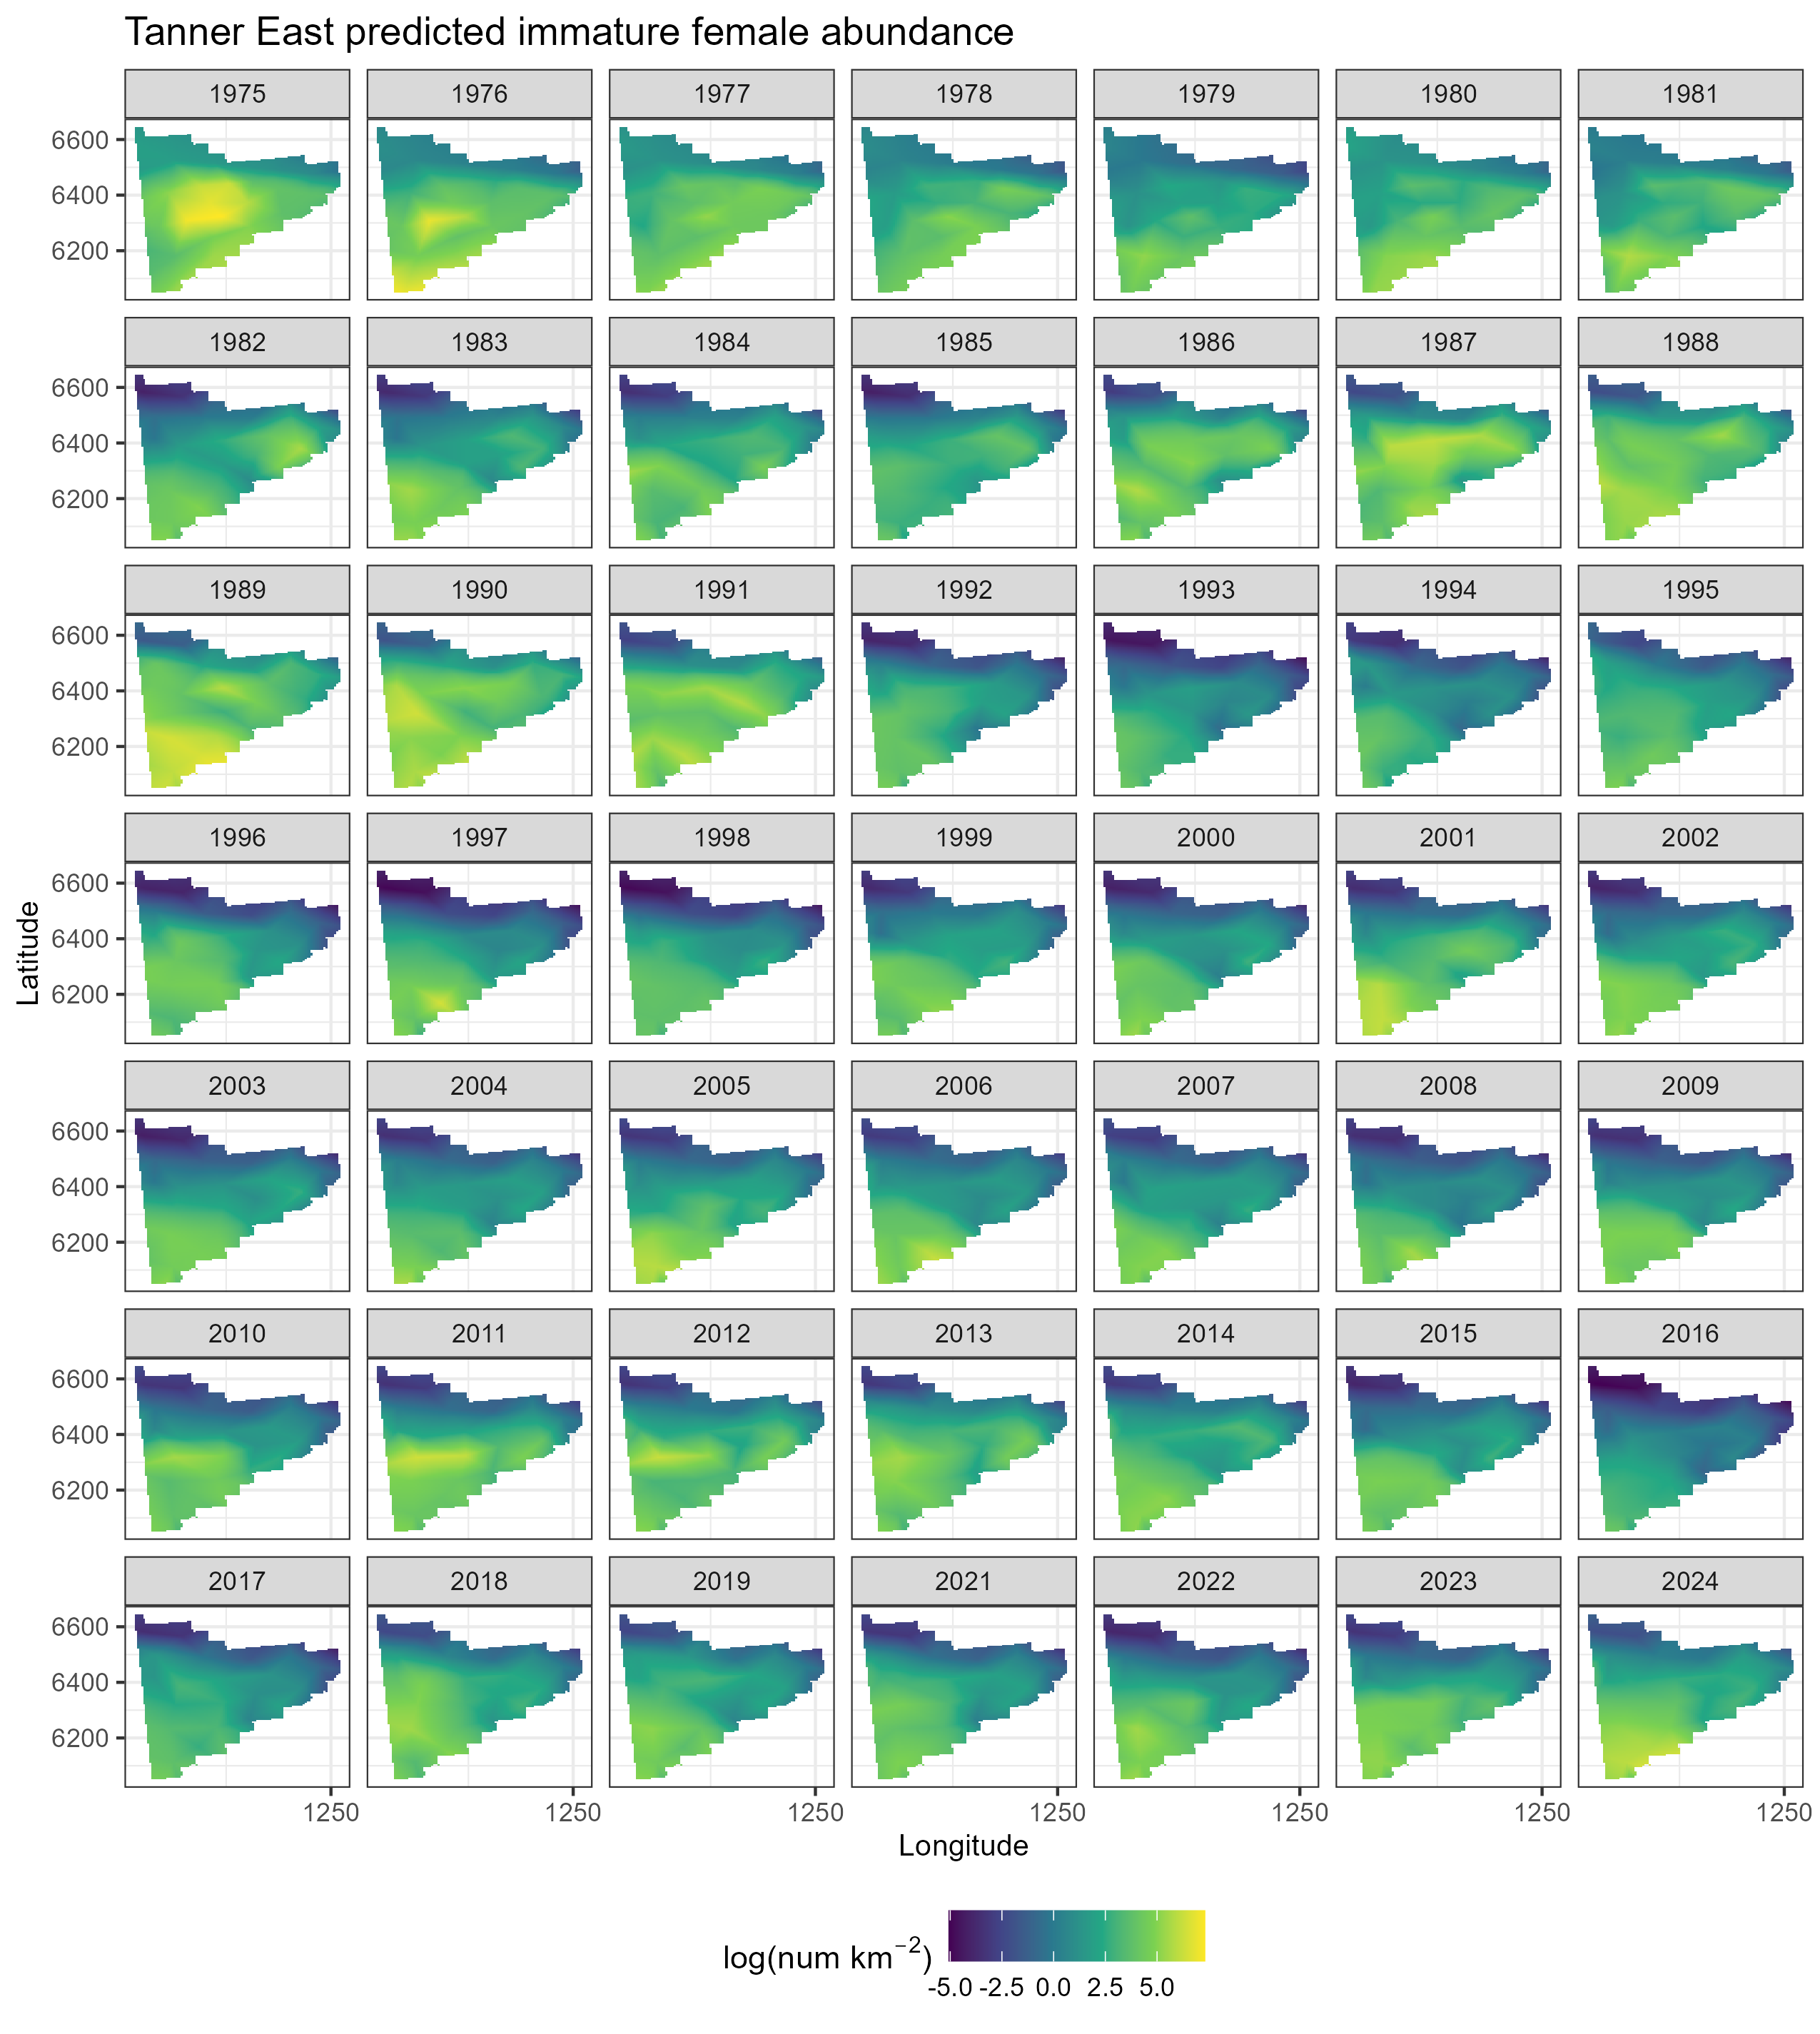
\includegraphics[width=1\linewidth,height=1\textheight]{../BAIRDI/Figures/TannerE_imfem_spatabund} 

}

\caption{Spatial predictions of immature female abundance east of 166° using NMFS summer bottom trawl survey data before 1982 and 1982 onward with a 50-knot mesh and a delta-gamma model family. Predictions from both of these periods/models are combined in this figure.}\label{fig:spatpred-abund-50-imfemE}
\end{figure}

\begin{figure}

{\centering 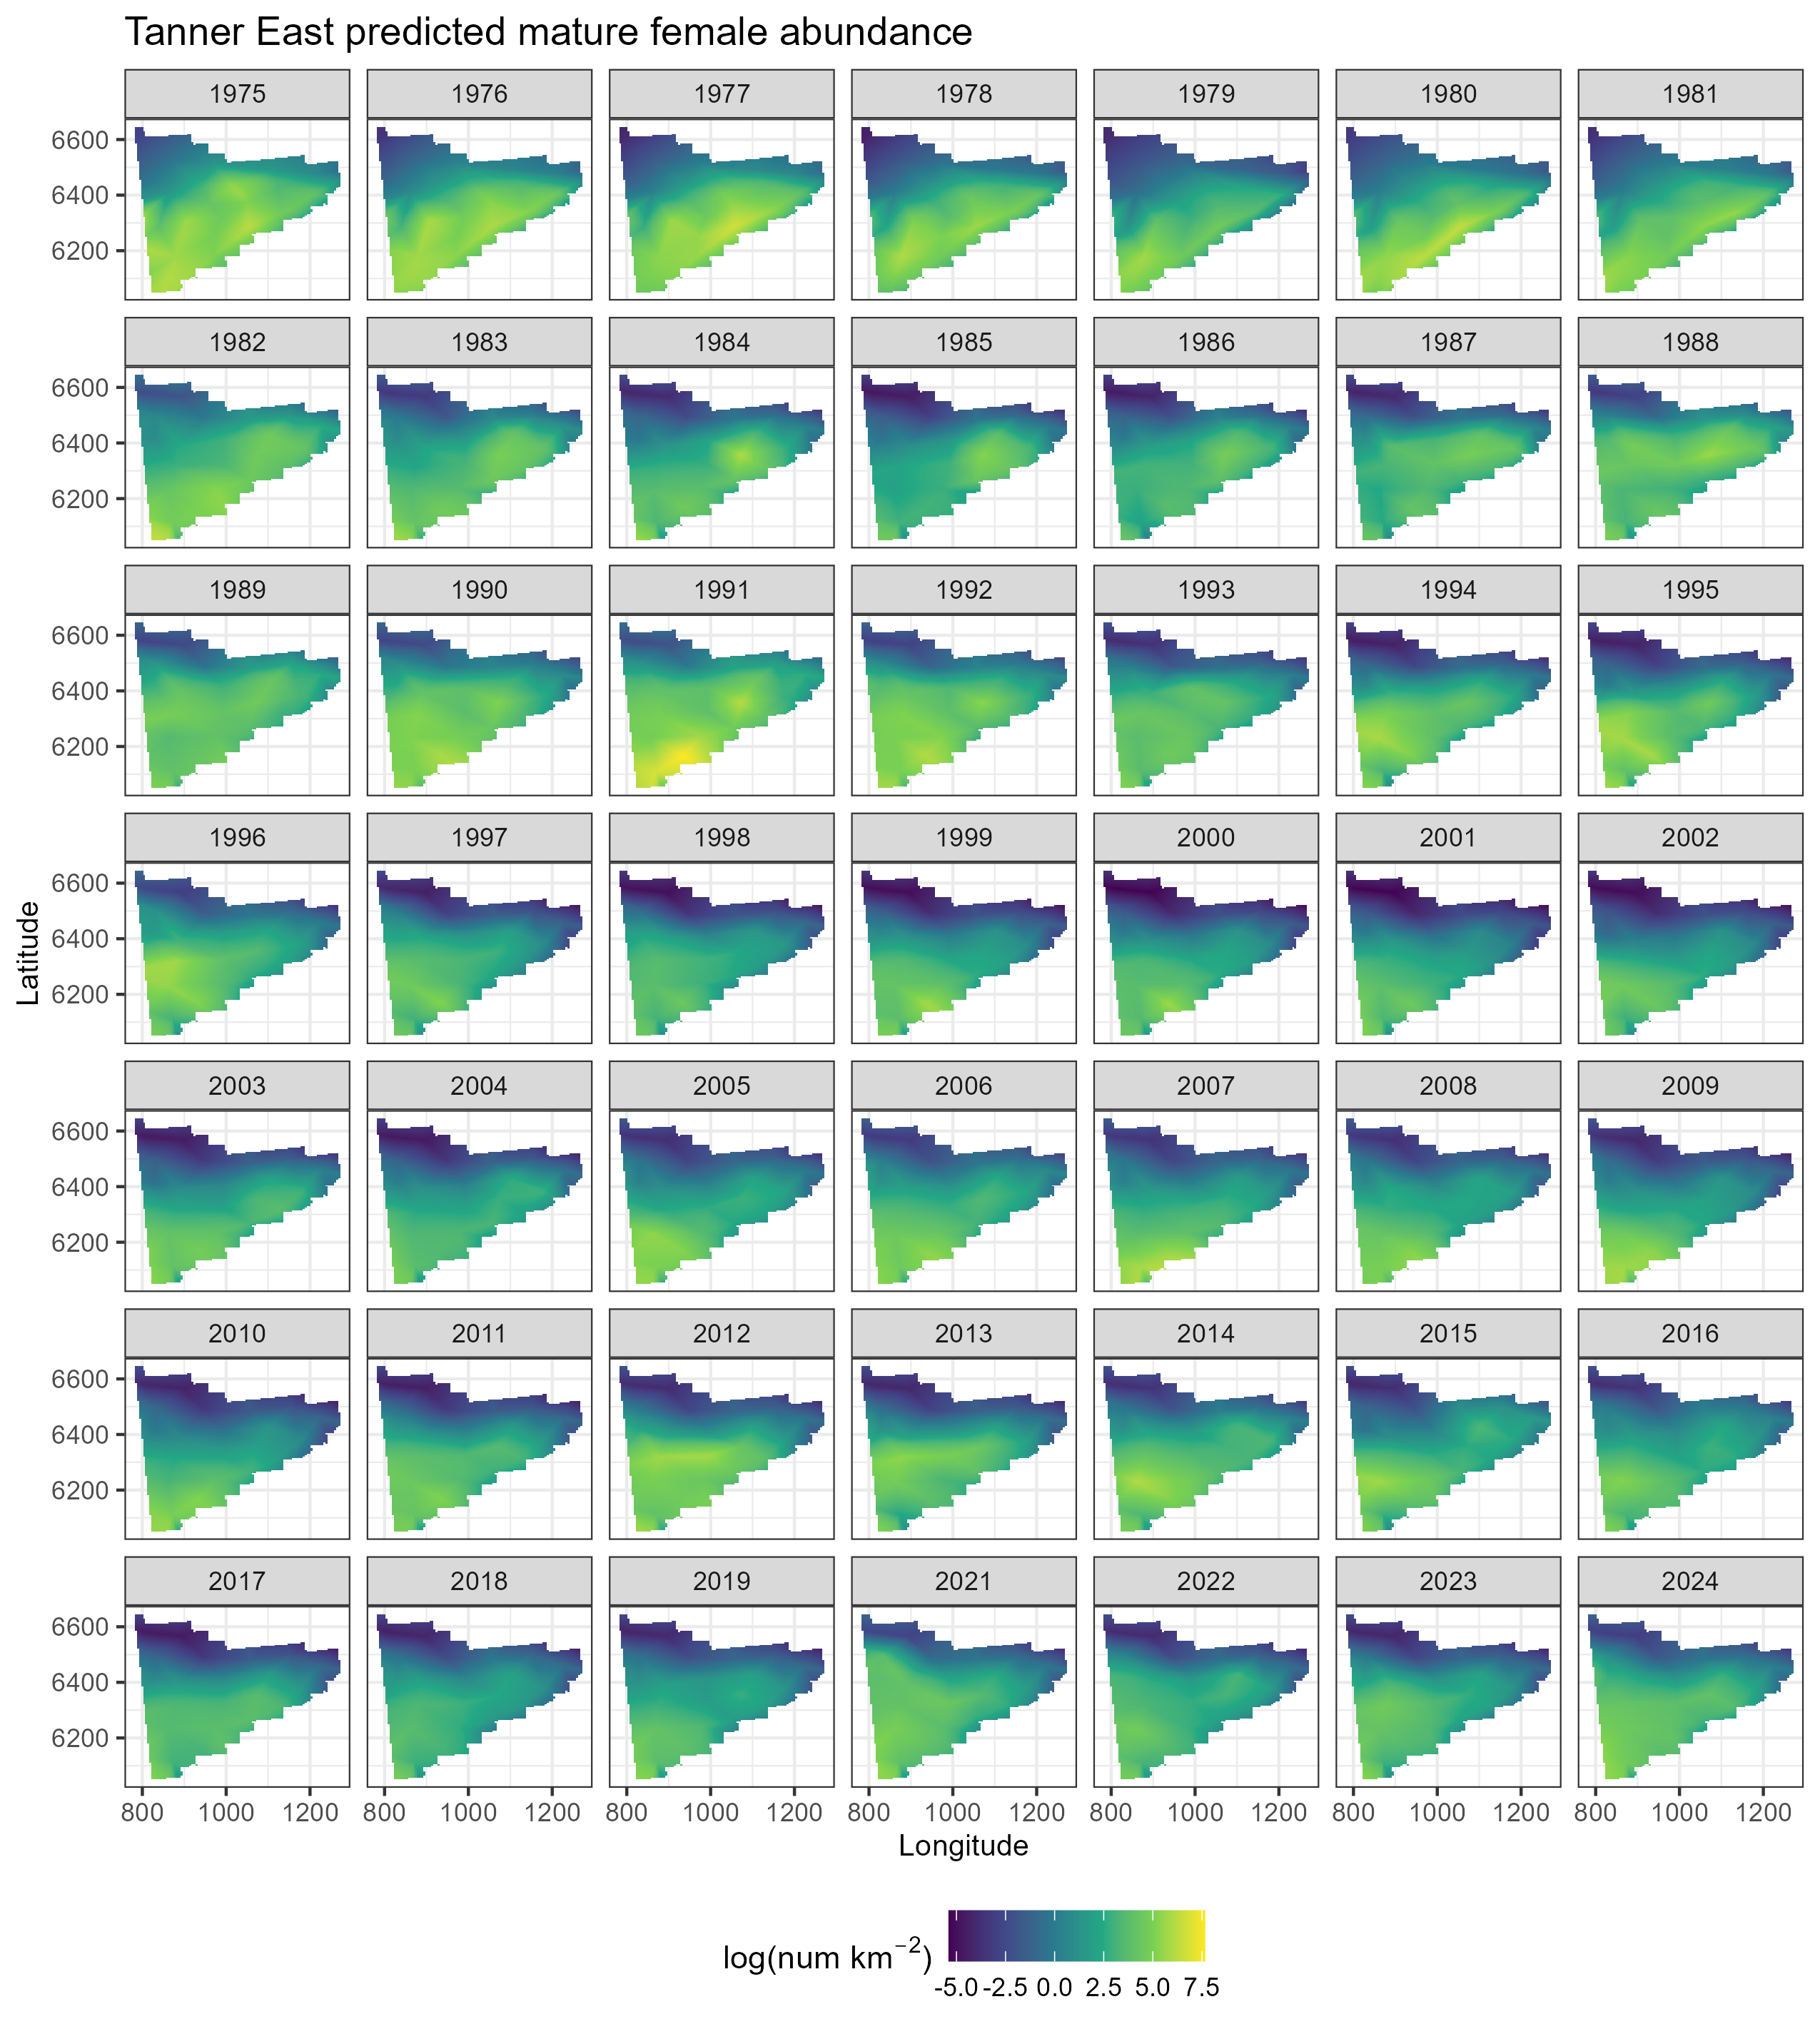
\includegraphics[width=1\linewidth,height=1\textheight]{../BAIRDI/Figures/TannerE_matfem_spatabund} 

}

\caption{Spatial predictions of mature female abundance east of 166° using NMFS summer bottom trawl survey data before 1982 and 1982 onward with a 50-knot mesh and a delta-gamma model family. Predictions from both of these periods/models are combined in this figure.}\label{fig:spatpred-abund-50-matfemE}
\end{figure}

\begin{figure}

{\centering 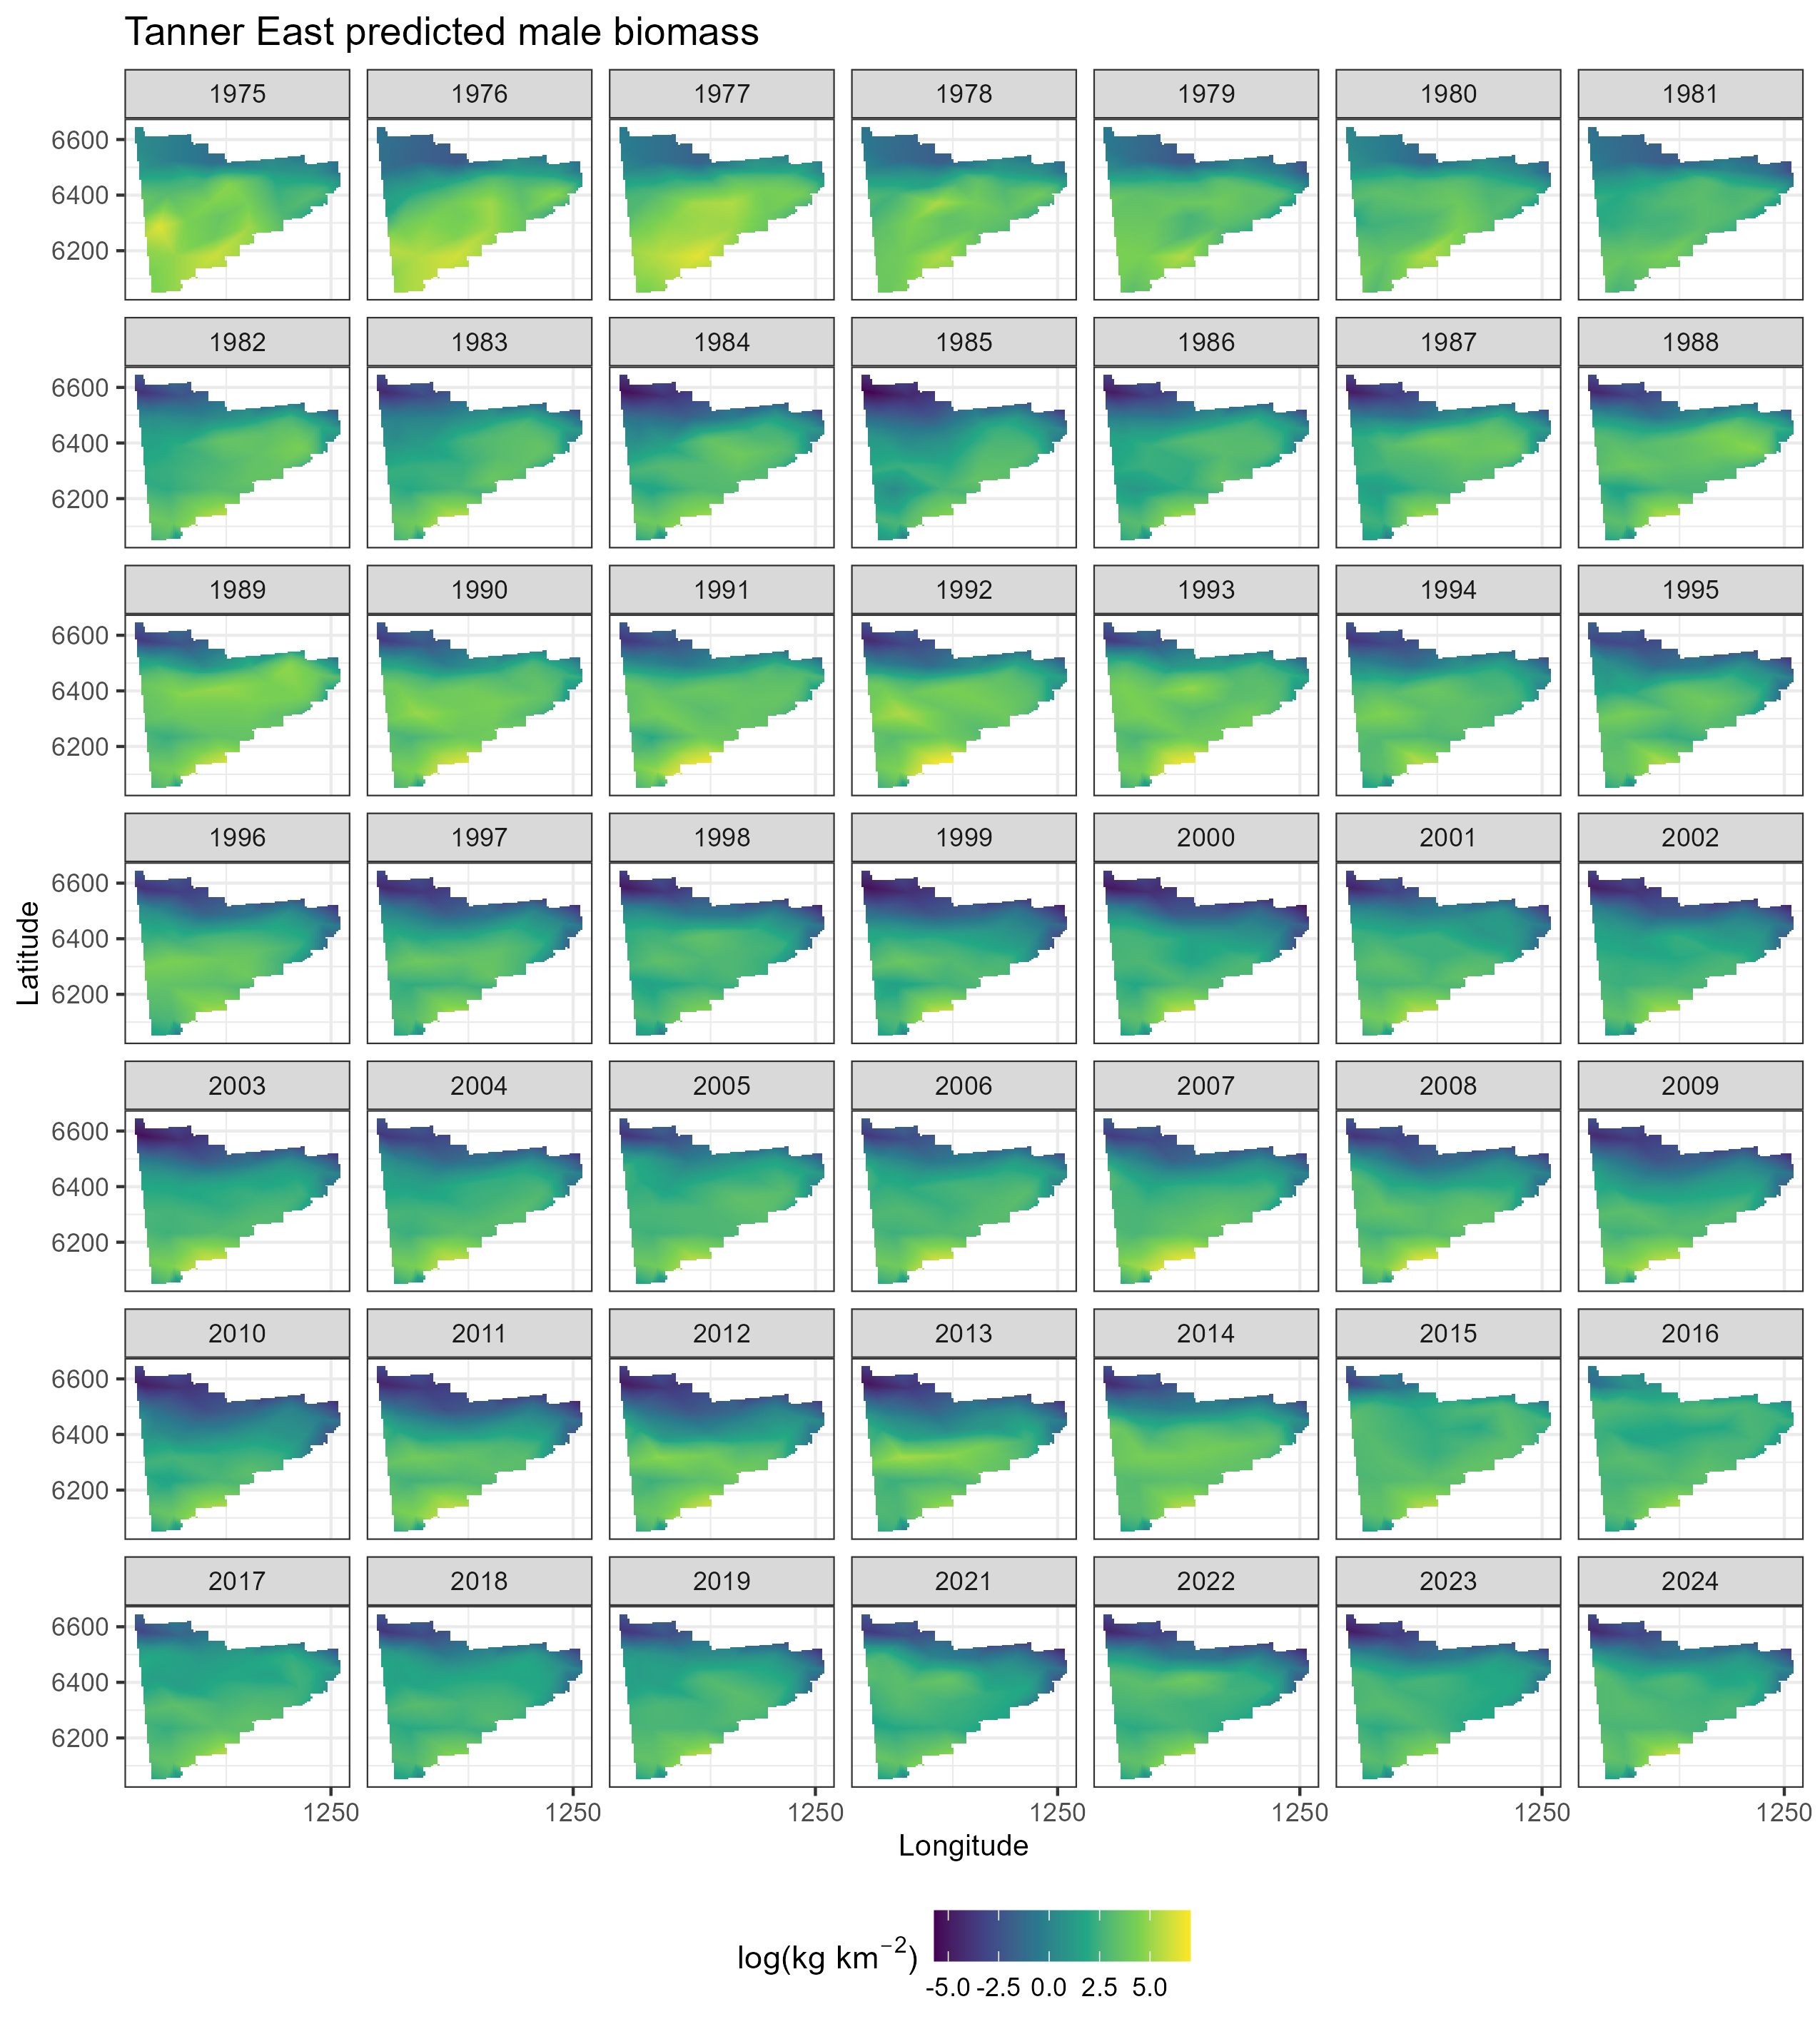
\includegraphics[width=1\linewidth,height=1\textheight]{../BAIRDI/Figures/TannerE_male_spatbio} 

}

\caption{Spatial predictions of male biomass east of 166° using NMFS summer bottom trawl survey data before 1982 and 1982 onward with a 50-knot mesh and a delta-gamma model family. Predictions from both of these periods/models are combined in this figure.}\label{fig:spatpred-bio-50-maleE}
\end{figure}

\begin{figure}

{\centering 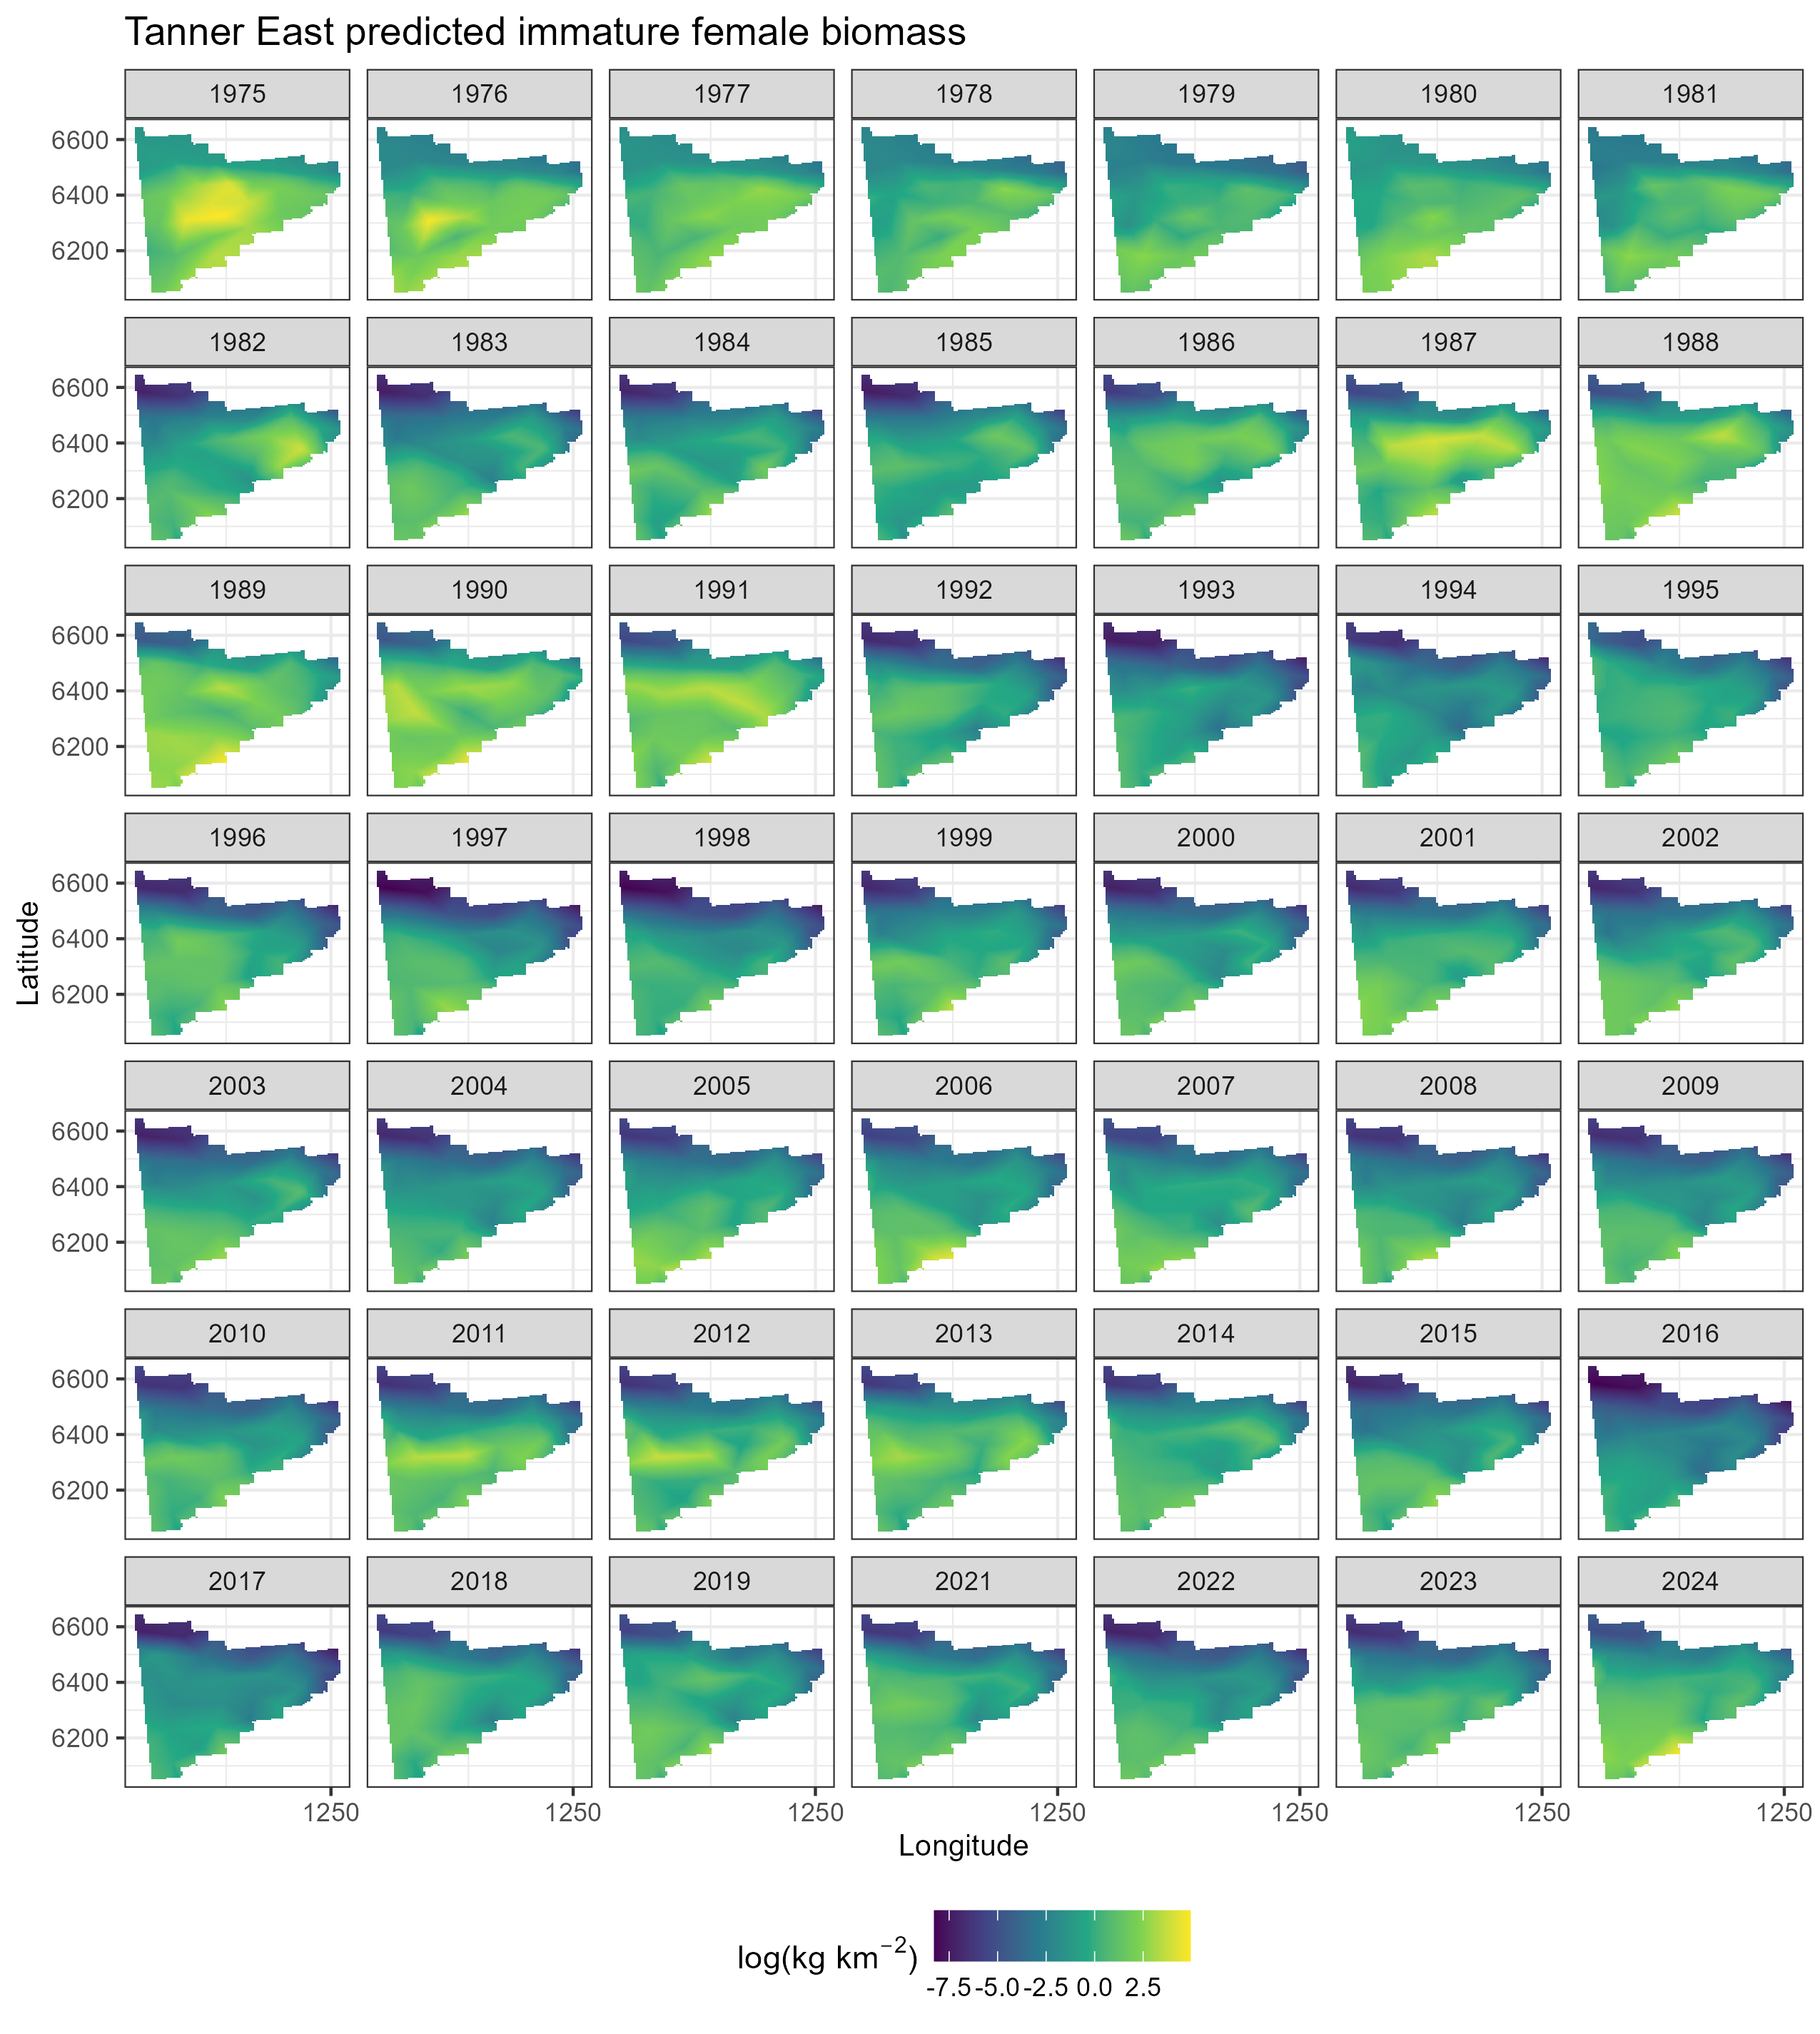
\includegraphics[width=1\linewidth,height=1\textheight]{../BAIRDI/Figures/TannerE_imfem_spatbio} 

}

\caption{Spatial predictions of immature female biomass east of 166° using NMFS summer bottom trawl survey data before 1982 and 1982 onward with a 50-knot mesh and a delta-gamma model family. Predictions from both of these periods/models are combined in this figure.}\label{fig:spatpred-bio-50-imfemE}
\end{figure}

\begin{figure}

{\centering 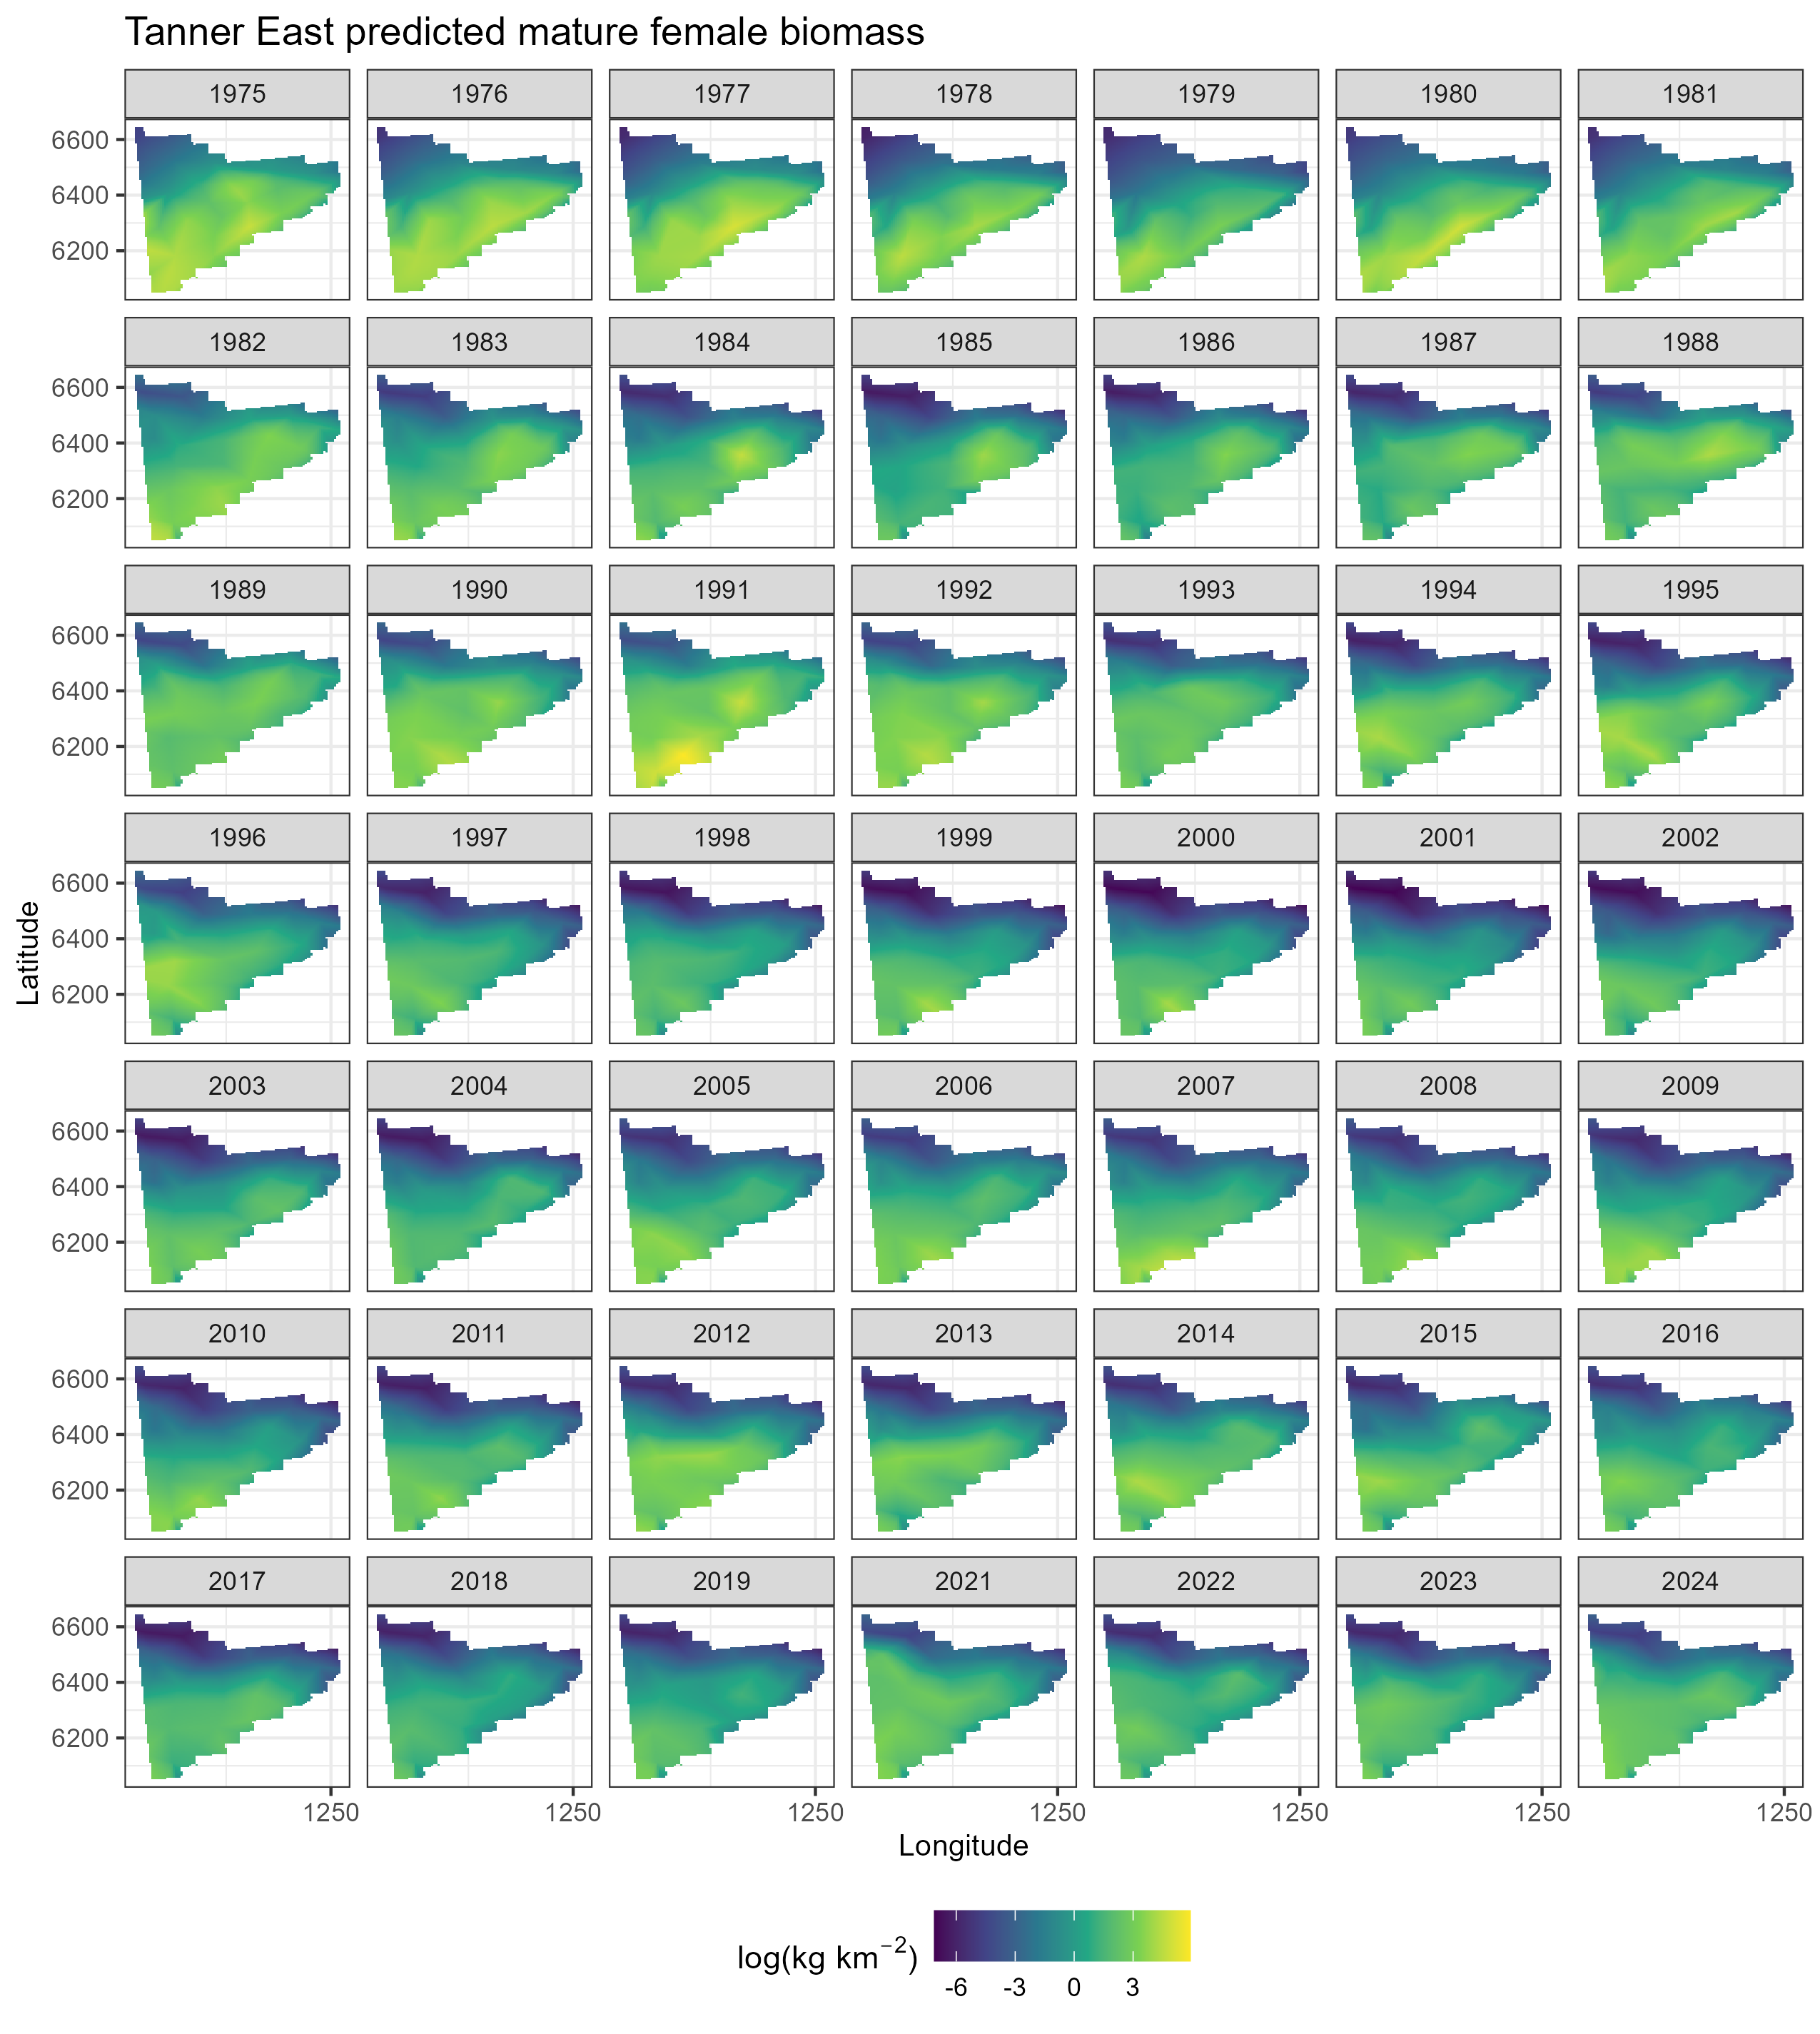
\includegraphics[width=1\linewidth,height=1\textheight]{../BAIRDI/Figures/TannerE_matfem_spatbio} 

}

\caption{Spatial predictions of mature female biomass east of 166° using NMFS summer bottom trawl survey data before 1982 and 1982 onward with a 50-knot mesh and a delta-gamma model family. Predictions from both of these periods/models are combined in this figure.}\label{fig:spatpred-bio-50-matfemE}
\end{figure}

\begin{figure}

{\centering \includegraphics[width=1\linewidth,height=1\textheight]{../BAIRDI/Figures/TannerWest.abundance.index} 

}

\caption{Estimated abundance (millions) for Tanner crab west of 166°. Colored lines represent abundance (±95\% CI) estimated by sdmTMB, with orange, blue, and pink denoting models fit with a 50-, 90-, and 120-knot mesh, respectively. Black points represent abundance (±95\% CI) estimated by the NMFS summer bottom trawl survey.}\label{fig:Westbairdi-abund-index}
\end{figure}

\begin{figure}

{\centering \includegraphics[width=1\linewidth,height=1\textheight]{../BAIRDI/Figures/TannerWest.biomass.index} 

}

\caption{Estimated biomass (tons) for eastern Bering Sea Tanner crab west of 166°. Colored lines represent abundance (±95\% CI) estimated by sdmTMB, with orange, blue, and pink denoting models fit with a 50-, 90-, and 120-knot mesh, respectively. Black points represent biomass (±95\% CI) estimated by the NMFS summer bottom trawl survey.}\label{fig:Westbairdi-bio-index}
\end{figure}

\begin{figure}

{\centering \includegraphics[width=1\linewidth,height=1\textheight]{../BAIRDI/Figures/TannerEast.abundance.index} 

}

\caption{Estimated abundance (millions) for Tanner crab east of 166°. Colored lines represent abundance (±95\% CI) estimated by sdmTMB, with orange, blue, and pink denoting models fit with a 50-, 90-, and 120-knot mesh, respectively. Black points represent abundance (±95\% CI) estimated by the NMFS summer bottom trawl survey.}\label{fig:Eastbairdi-abund-index}
\end{figure}

\begin{figure}

{\centering \includegraphics[width=1\linewidth,height=1\textheight]{../BAIRDI/Figures/TannerEast.biomass.index} 

}

\caption{Estimated biomass (tons) for eastern Bering Sea Tanner crab east of 166°. Colored lines represent abundance (±95\% CI) estimated by sdmTMB, with orange, blue, and pink denoting models fit with a 50-, 90-, and 120-knot mesh, respectively. Black points represent biomass (±95\% CI) estimated by the NMFS summer bottom trawl survey.}\label{fig:Eastbairdi-bio-index}
\end{figure}

\begin{figure}

{\centering \includegraphics[width=1\linewidth,height=1\textheight]{../BAIRDI/Figures/TannerW.abundance.sdmTMBVASTindex} 

}

\caption{Estimated abundance (millions; ±95\% CI) for Tanner crab west of 166° predicted using sdmTMB (pink) and VAST (blue). Both algorithms fit models using a delta-gamma family at 50 knots. Black points represent abundance (±95\% CI) estimated by the NMFS summer bottom trawl survey.}\label{fig:Westbairdi-abund-compare}
\end{figure}

\begin{figure}

{\centering \includegraphics[width=1\linewidth,height=1\textheight]{../BAIRDI/Figures/TannerW.biomass.sdmTMBVASTindex} 

}

\caption{Estimated biomass (tons; ±95\% CI) for Tanner crab west of 166° predicted using sdmTMB (pink) and VAST (blue). Both algorithms fit models using a delta-gamma family at 50 knots. Black points represent biomass (±95\% CI) estimated by the NMFS summer bottom trawl survey.}\label{fig:Westbairdi-bio-compare}
\end{figure}

\begin{figure}

{\centering \includegraphics[width=1\linewidth,height=1\textheight]{../BAIRDI/Figures/TannerE.abundance.sdmTMBVASTindex} 

}

\caption{Estimated abundance (millions; ±95\% CI) for Tanner crab east of 166° predicted using sdmTMB (pink) and VAST (blue). Both algorithms fit models using a delta-gamma family at 50 knots. Black points represent abundance (±95\% CI) estimated by the NMFS summer bottom trawl survey.}\label{fig:Eastbairdi-abund-compare}
\end{figure}

\begin{figure}

{\centering \includegraphics[width=1\linewidth,height=1\textheight]{../BAIRDI/Figures/TannerE.biomass.sdmTMBVASTindex} 

}

\caption{Estimated biomass (tons; ±95\% CI) for Tanner crab east of 166° predicted using sdmTMB (pink) and VAST (blue). Both algorithms fit models using a delta-gamma family at 50 knots. Black points represent biomass (±95\% CI) estimated by the NMFS summer bottom trawl survey.}\label{fig:Eastbairdi-bio-compare}
\end{figure}

\end{document}
